\documentclass[]{book}
\usepackage{lmodern}
\usepackage{amssymb,amsmath}
\usepackage{ifxetex,ifluatex}
\usepackage{fixltx2e} % provides \textsubscript
\ifnum 0\ifxetex 1\fi\ifluatex 1\fi=0 % if pdftex
  \usepackage[T1]{fontenc}
  \usepackage[utf8]{inputenc}
\else % if luatex or xelatex
  \ifxetex
    \usepackage{mathspec}
  \else
    \usepackage{fontspec}
  \fi
  \defaultfontfeatures{Ligatures=TeX,Scale=MatchLowercase}
\fi
% use upquote if available, for straight quotes in verbatim environments
\IfFileExists{upquote.sty}{\usepackage{upquote}}{}
% use microtype if available
\IfFileExists{microtype.sty}{%
\usepackage{microtype}
\UseMicrotypeSet[protrusion]{basicmath} % disable protrusion for tt fonts
}{}
\usepackage[margin=1in]{geometry}
\usepackage{hyperref}
\hypersetup{unicode=true,
            pdftitle={Data Science for Biological, Medical and Health Research: Notes for 432},
            pdfauthor={Thomas E. Love, Ph.D.},
            pdfborder={0 0 0},
            breaklinks=true}
\urlstyle{same}  % don't use monospace font for urls
\usepackage{natbib}
\bibliographystyle{apalike}
\usepackage{color}
\usepackage{fancyvrb}
\newcommand{\VerbBar}{|}
\newcommand{\VERB}{\Verb[commandchars=\\\{\}]}
\DefineVerbatimEnvironment{Highlighting}{Verbatim}{commandchars=\\\{\}}
% Add ',fontsize=\small' for more characters per line
\usepackage{framed}
\definecolor{shadecolor}{RGB}{248,248,248}
\newenvironment{Shaded}{\begin{snugshade}}{\end{snugshade}}
\newcommand{\KeywordTok}[1]{\textcolor[rgb]{0.13,0.29,0.53}{\textbf{#1}}}
\newcommand{\DataTypeTok}[1]{\textcolor[rgb]{0.13,0.29,0.53}{#1}}
\newcommand{\DecValTok}[1]{\textcolor[rgb]{0.00,0.00,0.81}{#1}}
\newcommand{\BaseNTok}[1]{\textcolor[rgb]{0.00,0.00,0.81}{#1}}
\newcommand{\FloatTok}[1]{\textcolor[rgb]{0.00,0.00,0.81}{#1}}
\newcommand{\ConstantTok}[1]{\textcolor[rgb]{0.00,0.00,0.00}{#1}}
\newcommand{\CharTok}[1]{\textcolor[rgb]{0.31,0.60,0.02}{#1}}
\newcommand{\SpecialCharTok}[1]{\textcolor[rgb]{0.00,0.00,0.00}{#1}}
\newcommand{\StringTok}[1]{\textcolor[rgb]{0.31,0.60,0.02}{#1}}
\newcommand{\VerbatimStringTok}[1]{\textcolor[rgb]{0.31,0.60,0.02}{#1}}
\newcommand{\SpecialStringTok}[1]{\textcolor[rgb]{0.31,0.60,0.02}{#1}}
\newcommand{\ImportTok}[1]{#1}
\newcommand{\CommentTok}[1]{\textcolor[rgb]{0.56,0.35,0.01}{\textit{#1}}}
\newcommand{\DocumentationTok}[1]{\textcolor[rgb]{0.56,0.35,0.01}{\textbf{\textit{#1}}}}
\newcommand{\AnnotationTok}[1]{\textcolor[rgb]{0.56,0.35,0.01}{\textbf{\textit{#1}}}}
\newcommand{\CommentVarTok}[1]{\textcolor[rgb]{0.56,0.35,0.01}{\textbf{\textit{#1}}}}
\newcommand{\OtherTok}[1]{\textcolor[rgb]{0.56,0.35,0.01}{#1}}
\newcommand{\FunctionTok}[1]{\textcolor[rgb]{0.00,0.00,0.00}{#1}}
\newcommand{\VariableTok}[1]{\textcolor[rgb]{0.00,0.00,0.00}{#1}}
\newcommand{\ControlFlowTok}[1]{\textcolor[rgb]{0.13,0.29,0.53}{\textbf{#1}}}
\newcommand{\OperatorTok}[1]{\textcolor[rgb]{0.81,0.36,0.00}{\textbf{#1}}}
\newcommand{\BuiltInTok}[1]{#1}
\newcommand{\ExtensionTok}[1]{#1}
\newcommand{\PreprocessorTok}[1]{\textcolor[rgb]{0.56,0.35,0.01}{\textit{#1}}}
\newcommand{\AttributeTok}[1]{\textcolor[rgb]{0.77,0.63,0.00}{#1}}
\newcommand{\RegionMarkerTok}[1]{#1}
\newcommand{\InformationTok}[1]{\textcolor[rgb]{0.56,0.35,0.01}{\textbf{\textit{#1}}}}
\newcommand{\WarningTok}[1]{\textcolor[rgb]{0.56,0.35,0.01}{\textbf{\textit{#1}}}}
\newcommand{\AlertTok}[1]{\textcolor[rgb]{0.94,0.16,0.16}{#1}}
\newcommand{\ErrorTok}[1]{\textcolor[rgb]{0.64,0.00,0.00}{\textbf{#1}}}
\newcommand{\NormalTok}[1]{#1}
\usepackage{longtable,booktabs}
\usepackage{graphicx,grffile}
\makeatletter
\def\maxwidth{\ifdim\Gin@nat@width>\linewidth\linewidth\else\Gin@nat@width\fi}
\def\maxheight{\ifdim\Gin@nat@height>\textheight\textheight\else\Gin@nat@height\fi}
\makeatother
% Scale images if necessary, so that they will not overflow the page
% margins by default, and it is still possible to overwrite the defaults
% using explicit options in \includegraphics[width, height, ...]{}
\setkeys{Gin}{width=\maxwidth,height=\maxheight,keepaspectratio}
\IfFileExists{parskip.sty}{%
\usepackage{parskip}
}{% else
\setlength{\parindent}{0pt}
\setlength{\parskip}{6pt plus 2pt minus 1pt}
}
\setlength{\emergencystretch}{3em}  % prevent overfull lines
\providecommand{\tightlist}{%
  \setlength{\itemsep}{0pt}\setlength{\parskip}{0pt}}
\setcounter{secnumdepth}{5}
% Redefines (sub)paragraphs to behave more like sections
\ifx\paragraph\undefined\else
\let\oldparagraph\paragraph
\renewcommand{\paragraph}[1]{\oldparagraph{#1}\mbox{}}
\fi
\ifx\subparagraph\undefined\else
\let\oldsubparagraph\subparagraph
\renewcommand{\subparagraph}[1]{\oldsubparagraph{#1}\mbox{}}
\fi

%%% Use protect on footnotes to avoid problems with footnotes in titles
\let\rmarkdownfootnote\footnote%
\def\footnote{\protect\rmarkdownfootnote}

%%% Change title format to be more compact
\usepackage{titling}

% Create subtitle command for use in maketitle
\newcommand{\subtitle}[1]{
  \posttitle{
    \begin{center}\large#1\end{center}
    }
}

\setlength{\droptitle}{-2em}
  \title{Data Science for Biological, Medical and Health Research: Notes for 432}
  \pretitle{\vspace{\droptitle}\centering\huge}
  \posttitle{\par}
  \author{Thomas E. Love, Ph.D.}
  \preauthor{\centering\large\emph}
  \postauthor{\par}
  \predate{\centering\large\emph}
  \postdate{\par}
  \date{Built 2018-02-01 17:10:42}

\usepackage{booktabs}
\usepackage{amsthm}
\makeatletter
\def\thm@space@setup{%
  \thm@preskip=8pt plus 2pt minus 4pt
  \thm@postskip=\thm@preskip
}
\makeatother

\usepackage{amsthm}
\newtheorem{theorem}{Theorem}[chapter]
\newtheorem{lemma}{Lemma}[chapter]
\theoremstyle{definition}
\newtheorem{definition}{Definition}[chapter]
\newtheorem{corollary}{Corollary}[chapter]
\newtheorem{proposition}{Proposition}[chapter]
\theoremstyle{definition}
\newtheorem{example}{Example}[chapter]
\theoremstyle{definition}
\newtheorem{exercise}{Exercise}[chapter]
\theoremstyle{remark}
\newtheorem*{remark}{Remark}
\newtheorem*{solution}{Solution}
\begin{document}
\maketitle

{
\setcounter{tocdepth}{1}
\tableofcontents
}
\chapter*{Introduction}\label{introduction}
\addcontentsline{toc}{chapter}{Introduction}

These Notes provide a series of examples using R to work through issues
that are likely to come up in PQHS/CRSP/MPHP 432.

While these Notes share some of the features of a textbook, they are
neither comprehensive nor completely original. The main purpose is to
give students in 432 a set of common materials on which to draw during
the course. In class, we will sometimes:

\begin{itemize}
\tightlist
\item
  reiterate points made in this document,
\item
  amplify what is here,
\item
  simplify the presentation of things done here,
\item
  use new examples to show some of the same techniques,
\item
  refer to issues not mentioned in this document,
\end{itemize}

but what we don't (always) do is follow these notes very precisely. We
assume instead that you will read the materials and try to learn from
them, just as you will attend classes and try to learn from them. We
welcome feedback of all kinds on this document or anything else. Just
email us at \texttt{431-help\ at\ case\ dot\ edu}, or submit a pull
request. Note that we still use \texttt{431-help} even though we're now
in 432.

What you will mostly find are brief explanations of a key idea or
summary, accompanied (most of the time) by R code and a demonstration of
the results of applying that code.

Everything you see here is available to you as HTML or PDF. You will
also have access to the R Markdown files, which contain the code which
generates everything in the document, including all of the R results. We
will demonstrate the use of R Markdown (this document is generated with
the additional help of an R package called bookdown) and R Studio (the
``program'' which we use to interface with the R language) in class.

To download the data and R code related to these notes, visit the Data
and Code section of \href{https://github.com/THOMASELOVE/432-2018}{the
432 course website}.

\chapter*{R Packages used in these
notes}\label{r-packages-used-in-these-notes}
\addcontentsline{toc}{chapter}{R Packages used in these notes}

Here, we'll load in the packages used in these notes.

\begin{Shaded}
\begin{Highlighting}[]
\KeywordTok{library}\NormalTok{(tableone)}
\KeywordTok{library}\NormalTok{(skimr)}
\KeywordTok{library}\NormalTok{(ggridges)}
\KeywordTok{library}\NormalTok{(magrittr)}
\KeywordTok{library}\NormalTok{(arm)}
\KeywordTok{library}\NormalTok{(rms)}
\KeywordTok{library}\NormalTok{(leaps)}
\KeywordTok{library}\NormalTok{(lars)}
\KeywordTok{library}\NormalTok{(simputation)}
\KeywordTok{library}\NormalTok{(modelr)}
\KeywordTok{library}\NormalTok{(broom)}
\KeywordTok{library}\NormalTok{(tidyverse)}
\end{Highlighting}
\end{Shaded}

\chapter*{Data used in these notes}\label{data-used-in-these-notes}
\addcontentsline{toc}{chapter}{Data used in these notes}

Here, we'll load in the data sets used in these notes.

\begin{Shaded}
\begin{Highlighting}[]
\NormalTok{fakestroke <-}\StringTok{ }\KeywordTok{read.csv}\NormalTok{(}\StringTok{"data/fakestroke.csv"}\NormalTok{) }\OperatorTok\StringTok{ }\NormalTok{tbl_df}
\NormalTok{bloodbrain <-}\StringTok{ }\KeywordTok{read.csv}\NormalTok{(}\StringTok{"data/bloodbrain.csv"}\NormalTok{) }\OperatorTok\StringTok{ }\NormalTok{tbl_df}
\NormalTok{smartcle1 <-}\StringTok{ }\KeywordTok{read.csv}\NormalTok{(}\StringTok{"data/smartcle1.csv"}\NormalTok{) }\OperatorTok\StringTok{ }\NormalTok{tbl_df}
\NormalTok{bonding <-}\StringTok{ }\KeywordTok{read.csv}\NormalTok{(}\StringTok{"data/bonding.csv"}\NormalTok{) }\OperatorTok\StringTok{ }\NormalTok{tbl_df}
\NormalTok{cortisol <-}\StringTok{ }\KeywordTok{read.csv}\NormalTok{(}\StringTok{"data/cortisol.csv"}\NormalTok{) }\OperatorTok\StringTok{ }\NormalTok{tbl_df}
\NormalTok{emphysema <-}\StringTok{ }\KeywordTok{read.csv}\NormalTok{(}\StringTok{"data/emphysema.csv"}\NormalTok{) }\OperatorTok\StringTok{ }\NormalTok{tbl_df}
\NormalTok{prost <-}\StringTok{ }\KeywordTok{read.csv}\NormalTok{(}\StringTok{"data/prost.csv"}\NormalTok{) }\OperatorTok\StringTok{ }\NormalTok{tbl_df}
\NormalTok{maleptsd <-}\StringTok{ }\KeywordTok{read.csv}\NormalTok{(}\StringTok{"data/maleptsd.csv"}\NormalTok{) }\OperatorTok\StringTok{ }\NormalTok{tbl_df}
\end{Highlighting}
\end{Shaded}

\chapter*{Special Functions used in these
notes}\label{special-functions-used-in-these-notes}
\addcontentsline{toc}{chapter}{Special Functions used in these notes}

\begin{Shaded}
\begin{Highlighting}[]
\NormalTok{specify_decimal <-}\StringTok{ }\ControlFlowTok{function}\NormalTok{(x, k) }\KeywordTok{format}\NormalTok{(}\KeywordTok{round}\NormalTok{(x, k), }\DataTypeTok{nsmall=}\NormalTok{k)}
\end{Highlighting}
\end{Shaded}

\chapter{Building Table 1}\label{building-table-1}

Many scientific articles involve direct comparison of results from
various exposures, perhaps treatments. In 431, we studied numerous
methods, including various sorts of hypothesis tests, confidence
intervals, and descriptive summaries, which can help us to understand
and compare outcomes in such a setting. One common approach is to
present what's often called Table 1. Table 1 provides a summary of the
characteristics of a sample, or of groups of samples, which is most
commonly used to help understand the nature of the data being compared.

\section{\texorpdfstring{Two examples from the \emph{New England Journal
of
Medicine}}{Two examples from the New England Journal of Medicine}}\label{two-examples-from-the-new-england-journal-of-medicine}

\subsection{A simple Table 1}\label{a-simple-table-1}

Table 1 is especially common in the context of clinical research.
Consider the excerpt below, from a January 2015 article in the \emph{New
England Journal of Medicine} \citep{Tolaney2015}.

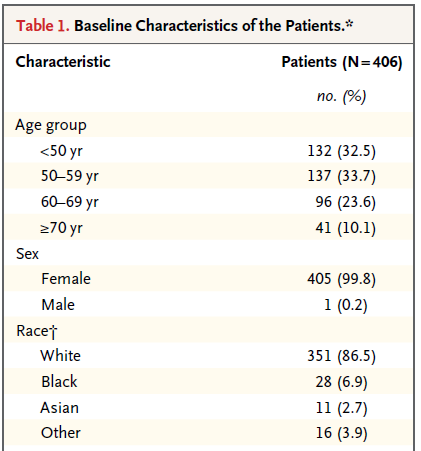
\includegraphics[width=0.5\linewidth]{images/Tolaney-snip1}

This (partial) table reports baseline characteristics on age group, sex
and race, describing 406 patients with HER2-positive\footnote{HER2 =
  human epidermal growth factor receptor type 2. Over-expression of this
  occurs in 15-20\% of invasive breast cancers, and has been associated
  with poor outcomes.} invasive breast cancer that began the protocol
therapy. Age, sex and race (along with severity of illness) are the most
commonly identified characteristics in a Table 1.

In addition to the measures shown in this excerpt, the full Table also
includes detailed information on the primary tumor for each patient,
including its size, nodal status and histologic grade. Footnotes tell us
that the percentages shown are subject to rounding, and may not total
100, and that the race information was self-reported.

\subsection{A group comparison}\label{a-group-comparison}

A more typical Table 1 involves a group comparison, for example in this
excerpt from \citet{Roy2008}. This Table 1 describes a multi-center
randomized clinical trial comparing two different approaches to caring
for patients with heart failure and atrial fibrillation\footnote{The
  complete Table 1 appears on pages 2668-2669 of \citet{Roy2008}, but I
  have only reproduced the first page and the footnote in this excerpt.}.

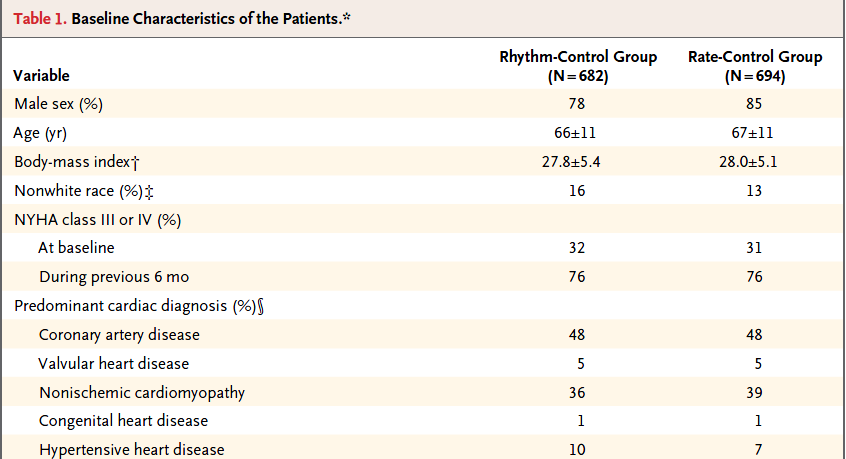
\includegraphics[width=0.9\linewidth]{images/Roy-snip1}

The article provides percentages, means and standard deviations across
groups, but note that it does not provide p values for the comparison of
baseline characteristics. This is a common feature of NEJM reports on
randomized clinical trials, where we anticipate that the two groups will
be well matched at baseline. Note that the patients in this study were
\emph{randomly} assigned to either the rhythm-control group or to the
rate-control group, using blocked randomizations stratified by study
center.

\section{The MR CLEAN trial}\label{the-mr-clean-trial}

\citet{Berkhemer2015} reported on the MR CLEAN trial, involving 500
patients with acute ischemic stroke caused by a proximal intracranial
arterial occlusion. The trial was conducted at 16 medical centers in the
Netherlands, where 233 were randomly assigned to the intervention
(intraarterial treatment plus usual care) and 267 to control (usual care
alone.) The primary outcome was the modified Rankin scale score at 90
days; this categorical scale measures functional outcome, with scores
ranging from 0 (no symptoms) to 6 (death). The fundamental conclusion of
\citet{Berkhemer2015} was that in patients with acute ischemic stroke
caused by a proximal intracranial occlusion of the anterior circulation,
intraarterial treatment administered within 6 hours after stroke onset
was effective and safe.

Here's the Table 1 from \citet{Berkhemer2015}.

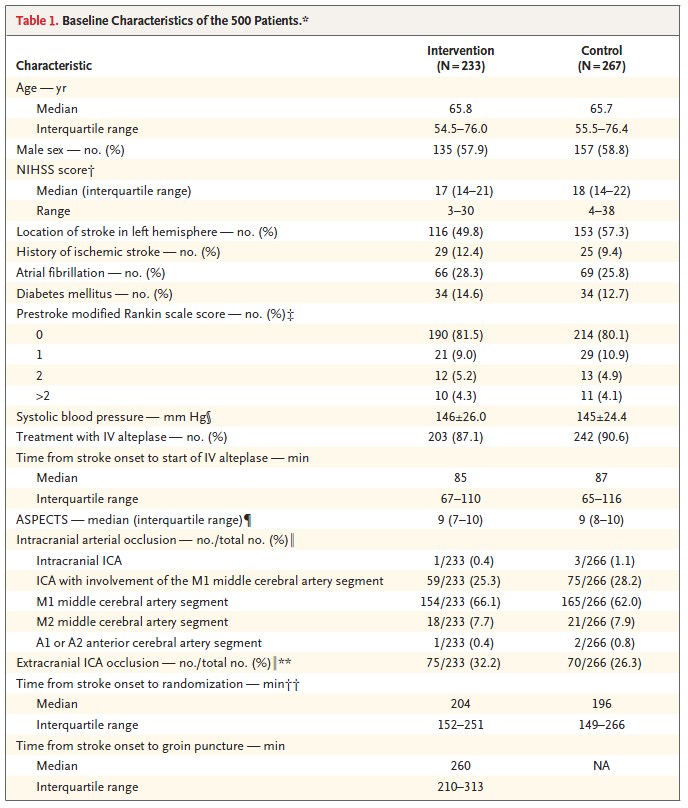
\includegraphics[width=0.9\linewidth]{images/Berkhemer-snip4complete}

The Table was accompanied by the following notes.

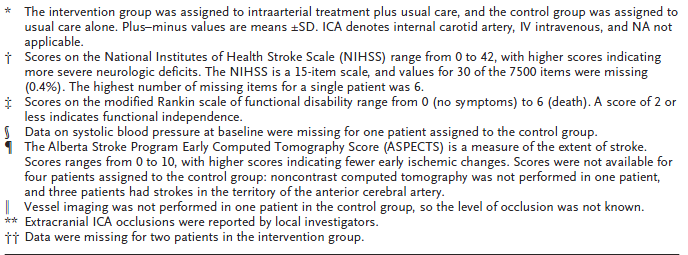
\includegraphics[width=0.9\linewidth]{images/Berkhemer-snip4notes}

\section{\texorpdfstring{Simulated \texttt{fakestroke}
data}{Simulated fakestroke data}}\label{simulated-fakestroke-data}

Consider the simulated data, available on the Data and Code page of
\href{https://github.com/THOMASELOVE/432-2018}{our course website} in
the \texttt{fakestroke.csv} file, which I built to let us mirror the
Table 1 for MR CLEAN \citep{Berkhemer2015}. The \texttt{fakestroke.csv}
file contains the following 18 variables for 500 patients.

\begin{longtable}[]{@{}rl@{}}
\toprule
\begin{minipage}[b]{0.16\columnwidth}\raggedleft\strut
Variable\strut
\end{minipage} & \begin{minipage}[b]{0.55\columnwidth}\raggedright\strut
Description\strut
\end{minipage}\tabularnewline
\midrule
\endhead
\begin{minipage}[t]{0.16\columnwidth}\raggedleft\strut
\texttt{studyid}\strut
\end{minipage} & \begin{minipage}[t]{0.55\columnwidth}\raggedright\strut
Study ID \# (z001 through z500)\strut
\end{minipage}\tabularnewline
\begin{minipage}[t]{0.16\columnwidth}\raggedleft\strut
\texttt{trt}\strut
\end{minipage} & \begin{minipage}[t]{0.55\columnwidth}\raggedright\strut
Treatment group (Intervention or Control)\strut
\end{minipage}\tabularnewline
\begin{minipage}[t]{0.16\columnwidth}\raggedleft\strut
\texttt{age}\strut
\end{minipage} & \begin{minipage}[t]{0.55\columnwidth}\raggedright\strut
Age in years\strut
\end{minipage}\tabularnewline
\begin{minipage}[t]{0.16\columnwidth}\raggedleft\strut
\texttt{sex}\strut
\end{minipage} & \begin{minipage}[t]{0.55\columnwidth}\raggedright\strut
Male or Female\strut
\end{minipage}\tabularnewline
\begin{minipage}[t]{0.16\columnwidth}\raggedleft\strut
\texttt{nihss}\strut
\end{minipage} & \begin{minipage}[t]{0.55\columnwidth}\raggedright\strut
NIH Stroke Scale Score (can range from 0-42; higher scores indicate more
severe neurological deficits)\strut
\end{minipage}\tabularnewline
\begin{minipage}[t]{0.16\columnwidth}\raggedleft\strut
\texttt{location}\strut
\end{minipage} & \begin{minipage}[t]{0.55\columnwidth}\raggedright\strut
Stroke Location - Left or Right Hemisphere\strut
\end{minipage}\tabularnewline
\begin{minipage}[t]{0.16\columnwidth}\raggedleft\strut
\texttt{hx.isch}\strut
\end{minipage} & \begin{minipage}[t]{0.55\columnwidth}\raggedright\strut
History of Ischemic Stroke (Yes/No)\strut
\end{minipage}\tabularnewline
\begin{minipage}[t]{0.16\columnwidth}\raggedleft\strut
\texttt{afib}\strut
\end{minipage} & \begin{minipage}[t]{0.55\columnwidth}\raggedright\strut
Atrial Fibrillation (1 = Yes, 0 = No)\strut
\end{minipage}\tabularnewline
\begin{minipage}[t]{0.16\columnwidth}\raggedleft\strut
\texttt{dm}\strut
\end{minipage} & \begin{minipage}[t]{0.55\columnwidth}\raggedright\strut
Diabetes Mellitus (1 = Yes, 0 = No)\strut
\end{minipage}\tabularnewline
\begin{minipage}[t]{0.16\columnwidth}\raggedleft\strut
\texttt{mrankin}\strut
\end{minipage} & \begin{minipage}[t]{0.55\columnwidth}\raggedright\strut
Pre-stroke modified Rankin scale score (0, 1, 2 or \textgreater{} 2)
indicating functional disability - complete range is 0 (no symptoms) to
6 (death)\strut
\end{minipage}\tabularnewline
\begin{minipage}[t]{0.16\columnwidth}\raggedleft\strut
\texttt{sbp}\strut
\end{minipage} & \begin{minipage}[t]{0.55\columnwidth}\raggedright\strut
Systolic blood pressure, in mm Hg\strut
\end{minipage}\tabularnewline
\begin{minipage}[t]{0.16\columnwidth}\raggedleft\strut
\texttt{iv.altep}\strut
\end{minipage} & \begin{minipage}[t]{0.55\columnwidth}\raggedright\strut
Treatment with IV alteplase (Yes/No)\strut
\end{minipage}\tabularnewline
\begin{minipage}[t]{0.16\columnwidth}\raggedleft\strut
\texttt{time.iv}\strut
\end{minipage} & \begin{minipage}[t]{0.55\columnwidth}\raggedright\strut
Time from stroke onset to start of IV alteplase (minutes) if
iv.altep=Yes\strut
\end{minipage}\tabularnewline
\begin{minipage}[t]{0.16\columnwidth}\raggedleft\strut
\texttt{aspects}\strut
\end{minipage} & \begin{minipage}[t]{0.55\columnwidth}\raggedright\strut
Alberta Stroke Program Early Computed Tomography score, which measures
extent of stroke from 0 - 10; higher scores indicate fewer early
ischemic changes\strut
\end{minipage}\tabularnewline
\begin{minipage}[t]{0.16\columnwidth}\raggedleft\strut
\texttt{ia.occlus}\strut
\end{minipage} & \begin{minipage}[t]{0.55\columnwidth}\raggedright\strut
Intracranial arterial occlusion, based on vessel imaging - five
categories\footnotemark{}\strut
\end{minipage}
\footnotetext{The five categories are Intracranial ICA, ICA with
  involvement of the M1 middle cerebral artery segment, M1 middle
  cerebral artery segment, M2 middle cerebral artery segment, A1 or A2
  anterior cerebral artery segment}\tabularnewline
\begin{minipage}[t]{0.16\columnwidth}\raggedleft\strut
\texttt{extra.ica}\strut
\end{minipage} & \begin{minipage}[t]{0.55\columnwidth}\raggedright\strut
Extracranial ICA occlusion (1 = Yes, 0 = No)\strut
\end{minipage}\tabularnewline
\begin{minipage}[t]{0.16\columnwidth}\raggedleft\strut
\texttt{time.rand}\strut
\end{minipage} & \begin{minipage}[t]{0.55\columnwidth}\raggedright\strut
Time from stroke onset to study randomization, in minutes\strut
\end{minipage}\tabularnewline
\begin{minipage}[t]{0.16\columnwidth}\raggedleft\strut
\texttt{time.punc}\strut
\end{minipage} & \begin{minipage}[t]{0.55\columnwidth}\raggedright\strut
Time from stroke onset to groin puncture, in minutes (only if
Intervention)\strut
\end{minipage}\tabularnewline
\bottomrule
\end{longtable}

Here's a quick look at the simulated data in \texttt{fakestroke}.

\begin{Shaded}
\begin{Highlighting}[]
\NormalTok{fakestroke}
\end{Highlighting}
\end{Shaded}

\begin{verbatim}
# A tibble: 500 x 18
   studyid trt        age sex   nihss location hx.isch  afib    dm mrankin
   <fct>   <fct>    <dbl> <fct> <int> <fct>    <fct>   <int> <int> <fct>  
 1 z001    Control   53.0 Male     21 Right    No          0     0 2      
 2 z002    Interve~  51.0 Male     23 Left     No          1     0 0      
 3 z003    Control   68.0 Fema~    11 Right    No          0     0 0      
 4 z004    Control   28.0 Male     22 Left     No          0     0 0      
 5 z005    Control   91.0 Male     24 Right    No          0     0 0      
 6 z006    Control   34.0 Fema~    18 Left     No          0     0 2      
 7 z007    Interve~  75.0 Male     25 Right    No          0     0 0      
 8 z008    Control   89.0 Fema~    18 Right    No          0     0 0      
 9 z009    Control   75.0 Male     25 Left     No          1     0 2      
10 z010    Interve~  26.0 Fema~    27 Right    No          0     0 0      
# ... with 490 more rows, and 8 more variables: sbp <int>, iv.altep <fct>,
#   time.iv <int>, aspects <int>, ia.occlus <fct>, extra.ica <int>,
#   time.rand <int>, time.punc <int>
\end{verbatim}

\section{\texorpdfstring{Building Table 1 for \texttt{fakestroke}:
Attempt
1}{Building Table 1 for fakestroke: Attempt 1}}\label{building-table-1-for-fakestroke-attempt-1}

Our goal, then, is to take the data in \texttt{fakestroke.csv} and use
it to generate a Table 1 for the study that compares the 233 patients in
the Intervention group to the 267 patients in the Control group, on all
of the other variables (except study ID \#) available. I'll use the
\texttt{tableone} package of functions available in R to help me
complete this task. We'll make a first attempt, using the
\texttt{CreateTableOne} function in the \texttt{tableone} package. To
use the function, we'll need to specify:

\begin{itemize}
\tightlist
\item
  the \texttt{vars} or variables we want to place in the rows of our
  Table 1 (which will include just about everything in the
  \texttt{fakestroke} data except the \texttt{studyid} code and the
  \texttt{trt} variable for which we have other plans, and the
  \texttt{time.punc} which applies only to subjects in the Intervention
  group.)

  \begin{itemize}
  \tightlist
  \item
    A useful trick here is to use the \texttt{dput} function,
    specifically something like \texttt{dput(names(fakestroke))} can be
    used to generate a list of all of the variables included in the
    \texttt{fakestroke} tibble, and then this can be copied and pasted
    into the \texttt{vars} specification, saving some typing.
  \end{itemize}
\item
  the \texttt{strata} which indicates the levels want to use in the
  columns of our Table 1 (for us, that's \texttt{trt})
\end{itemize}

\begin{Shaded}
\begin{Highlighting}[]
\NormalTok{fs.vars <-}\StringTok{ }\KeywordTok{c}\NormalTok{(}\StringTok{"age"}\NormalTok{, }\StringTok{"sex"}\NormalTok{, }\StringTok{"nihss"}\NormalTok{, }\StringTok{"location"}\NormalTok{, }
          \StringTok{"hx.isch"}\NormalTok{, }\StringTok{"afib"}\NormalTok{, }\StringTok{"dm"}\NormalTok{, }\StringTok{"mrankin"}\NormalTok{, }\StringTok{"sbp"}\NormalTok{,}
          \StringTok{"iv.altep"}\NormalTok{, }\StringTok{"time.iv"}\NormalTok{, }\StringTok{"aspects"}\NormalTok{, }
          \StringTok{"ia.occlus"}\NormalTok{, }\StringTok{"extra.ica"}\NormalTok{, }\StringTok{"time.rand"}\NormalTok{)}

\NormalTok{fs.trt <-}\StringTok{ }\KeywordTok{c}\NormalTok{(}\StringTok{"trt"}\NormalTok{)}

\NormalTok{att1 <-}\StringTok{ }\KeywordTok{CreateTableOne}\NormalTok{(}\DataTypeTok{data =}\NormalTok{ fakestroke, }
                       \DataTypeTok{vars =}\NormalTok{ fs.vars, }
                       \DataTypeTok{strata =}\NormalTok{ fs.trt)}
\KeywordTok{print}\NormalTok{(att1)}
\end{Highlighting}
\end{Shaded}

\begin{verbatim}
                       Stratified by trt
                        Control        Intervention   p      test
  n                        267            233                    
  age (mean (sd))        65.38 (16.10)  63.93 (18.09)  0.343     
  sex = Male (%)           157 (58.8)     135 (57.9)   0.917     
  nihss (mean (sd))      18.08 (4.32)   17.97 (5.04)   0.787     
  location = Right (%)     114 (42.7)     117 (50.2)   0.111     
  hx.isch = Yes (%)         25 ( 9.4)      29 (12.4)   0.335     
  afib (mean (sd))        0.26 (0.44)    0.28 (0.45)   0.534     
  dm (mean (sd))          0.13 (0.33)    0.12 (0.33)   0.923     
  mrankin (%)                                          0.922     
     > 2                    11 ( 4.1)      10 ( 4.3)             
     0                     214 (80.1)     190 (81.5)             
     1                      29 (10.9)      21 ( 9.0)             
     2                      13 ( 4.9)      12 ( 5.2)             
  sbp (mean (sd))       145.00 (24.40) 146.03 (26.00)  0.647     
  iv.altep = Yes (%)       242 (90.6)     203 (87.1)   0.267     
  time.iv (mean (sd))    87.96 (26.01)  98.22 (45.48)  0.003     
  aspects (mean (sd))     8.65 (1.47)    8.35 (1.64)   0.033     
  ia.occlus (%)                                        0.795     
     A1 or A2                2 ( 0.8)       1 ( 0.4)             
     ICA with M1            75 (28.2)      59 (25.3)             
     Intracranial ICA        3 ( 1.1)       1 ( 0.4)             
     M1                    165 (62.0)     154 (66.1)             
     M2                     21 ( 7.9)      18 ( 7.7)             
  extra.ica (mean (sd))   0.26 (0.44)    0.32 (0.47)   0.150     
  time.rand (mean (sd)) 213.88 (70.29) 202.51 (57.33)  0.051     
\end{verbatim}

\subsection{Some of this is very useful, and other parts need to be
fixed.}\label{some-of-this-is-very-useful-and-other-parts-need-to-be-fixed.}

\begin{enumerate}
\def\labelenumi{\arabic{enumi}.}
\tightlist
\item
  The 1/0 variables (\texttt{afib}, \texttt{dm}, \texttt{extra.ica})
  might be better if they were treated as the factors they are, and
  reported as the Yes/No variables are reported, with counts and
  percentages rather than with means and standard deviations.
\item
  In some cases, we may prefer to re-order the levels of the categorical
  (factor) variables, particularly the \texttt{mrankin} variable, but
  also the \texttt{ia.occlus} variable. It would also be more typical to
  put the Intervention group to the left and the Control group to the
  right, so we may need to adjust our \texttt{trt} variable's levels
  accordingly.
\item
  For each of the quantitative variables (\texttt{age}, \texttt{nihss},
  \texttt{sbp}, \texttt{time.iv}, \texttt{aspects}, \texttt{extra.ica},
  \texttt{time.rand} and \texttt{time.punc}) we should make a decision
  whether a summary with mean and standard deviation is appropriate, or
  whether we should instead summarize with, say, the median and
  quartiles. A mean and standard deviation really only yields an
  appropriate summary when the data are least approximately Normally
  distributed. This will make the \emph{p} values a bit more reasonable,
  too. The \texttt{test} column in the first attempt will soon have
  something useful to tell us.
\item
  If we'd left in the \texttt{time.punc} variable, we'd get some
  warnings, having to do with the fact that \texttt{time.punc} is only
  relevant to patients in the Intervention group.
\end{enumerate}

\subsection{\texorpdfstring{\texttt{fakestroke} Cleaning Up Categorical
Variables}{fakestroke Cleaning Up Categorical Variables}}\label{fakestroke-cleaning-up-categorical-variables}

Let's specify each of the categorical variables as categorical
explicitly. This helps the \texttt{CreateTableOne} function treat them
appropriately, and display them with counts and percentages. This
includes all of the 1/0, Yes/No and multi-categorical variables.

\begin{Shaded}
\begin{Highlighting}[]
\NormalTok{fs.factorvars <-}\StringTok{ }\KeywordTok{c}\NormalTok{(}\StringTok{"sex"}\NormalTok{, }\StringTok{"location"}\NormalTok{, }\StringTok{"hx.isch"}\NormalTok{, }\StringTok{"afib"}\NormalTok{, }\StringTok{"dm"}\NormalTok{, }
                   \StringTok{"mrankin"}\NormalTok{, }\StringTok{"iv.altep"}\NormalTok{, }\StringTok{"ia.occlus"}\NormalTok{, }\StringTok{"extra.ica"}\NormalTok{)}
\end{Highlighting}
\end{Shaded}

Then we simply add a \texttt{factorVars\ =\ fs.factorvars} call to the
\texttt{CreateTableOne} function.

We also want to re-order some of those categorical variables, so that
the levels are more useful to us. Specifically, we want to:

\begin{itemize}
\tightlist
\item
  place Intervention before Control in the \texttt{trt} variable,
\item
  reorder the \texttt{mrankin} scale as 0, 1, 2, \textgreater{} 2, and
\item
  rearrange the \texttt{ia.occlus} variable to the order\footnote{We
    might also have considered reordering the \texttt{ia.occlus} factor
    by its frequency, using the \texttt{fct\_infreq} function} presented
  in \citet{Berkhemer2015}.
\end{itemize}

To accomplish this, we'll use the \texttt{fct\_relevel} function from
the \texttt{forcats} package (loaded with the rest of the core
\texttt{tidyverse} packages) to reorder our levels manually.

\begin{Shaded}
\begin{Highlighting}[]
\NormalTok{fakestroke <-}\StringTok{ }\NormalTok{fakestroke }\OperatorTok
\StringTok{    }\KeywordTok{mutate}\NormalTok{(}\DataTypeTok{trt =} \KeywordTok{fct_relevel}\NormalTok{(trt, }\StringTok{"Intervention"}\NormalTok{, }\StringTok{"Control"}\NormalTok{),}
           \DataTypeTok{mrankin =} \KeywordTok{fct_relevel}\NormalTok{(mrankin, }\StringTok{"0"}\NormalTok{, }\StringTok{"1"}\NormalTok{, }\StringTok{"2"}\NormalTok{, }\StringTok{"> 2"}\NormalTok{),}
           \DataTypeTok{ia.occlus =} \KeywordTok{fct_relevel}\NormalTok{(ia.occlus, }\StringTok{"Intracranial ICA"}\NormalTok{, }
                                   \StringTok{"ICA with M1"}\NormalTok{, }\StringTok{"M1"}\NormalTok{, }\StringTok{"M2"}\NormalTok{, }
                                   \StringTok{"A1 or A2"}\NormalTok{)}
\NormalTok{           ) }
\end{Highlighting}
\end{Shaded}

\section{\texorpdfstring{\texttt{fakestroke} Table 1: Attempt
2}{fakestroke Table 1: Attempt 2}}\label{fakestroke-table-1-attempt-2}

\begin{Shaded}
\begin{Highlighting}[]
\NormalTok{att2 <-}\StringTok{ }\KeywordTok{CreateTableOne}\NormalTok{(}\DataTypeTok{data =}\NormalTok{ fakestroke, }
                       \DataTypeTok{vars =}\NormalTok{ fs.vars,}
                       \DataTypeTok{factorVars =}\NormalTok{ fs.factorvars,}
                       \DataTypeTok{strata =}\NormalTok{ fs.trt)}
\KeywordTok{print}\NormalTok{(att2)}
\end{Highlighting}
\end{Shaded}

\begin{verbatim}
                       Stratified by trt
                        Intervention   Control        p      test
  n                        233            267                    
  age (mean (sd))        63.93 (18.09)  65.38 (16.10)  0.343     
  sex = Male (%)           135 (57.9)     157 (58.8)   0.917     
  nihss (mean (sd))      17.97 (5.04)   18.08 (4.32)   0.787     
  location = Right (%)     117 (50.2)     114 (42.7)   0.111     
  hx.isch = Yes (%)         29 (12.4)      25 ( 9.4)   0.335     
  afib = 1 (%)              66 (28.3)      69 (25.8)   0.601     
  dm = 1 (%)                29 (12.4)      34 (12.7)   1.000     
  mrankin (%)                                          0.922     
     0                     190 (81.5)     214 (80.1)             
     1                      21 ( 9.0)      29 (10.9)             
     2                      12 ( 5.2)      13 ( 4.9)             
     > 2                    10 ( 4.3)      11 ( 4.1)             
  sbp (mean (sd))       146.03 (26.00) 145.00 (24.40)  0.647     
  iv.altep = Yes (%)       203 (87.1)     242 (90.6)   0.267     
  time.iv (mean (sd))    98.22 (45.48)  87.96 (26.01)  0.003     
  aspects (mean (sd))     8.35 (1.64)    8.65 (1.47)   0.033     
  ia.occlus (%)                                        0.795     
     Intracranial ICA        1 ( 0.4)       3 ( 1.1)             
     ICA with M1            59 (25.3)      75 (28.2)             
     M1                    154 (66.1)     165 (62.0)             
     M2                     18 ( 7.7)      21 ( 7.9)             
     A1 or A2                1 ( 0.4)       2 ( 0.8)             
  extra.ica = 1 (%)         75 (32.2)      70 (26.3)   0.179     
  time.rand (mean (sd)) 202.51 (57.33) 213.88 (70.29)  0.051     
\end{verbatim}

The categorical data presentation looks much improved.

\subsection{What summaries should we
show?}\label{what-summaries-should-we-show}

Now, we'll move on to the issue of making a decision about what type of
summary to show for the quantitative variables. Since the
\texttt{fakestroke} data are just simulated and only match the summary
statistics of the original results, not the details, we'll adopt the
decisions made by \citet{Berkhemer2015}, which were to use medians and
interquartile ranges to summarize the distributions of all of the
continuous variables \textbf{except} systolic blood pressure.

\begin{itemize}
\tightlist
\item
  Specifying certain quantitative variables as \emph{non-normal} causes
  R to show them with medians and the 25th and 75th percentiles, rather
  than means and standard deviations, and also causes those variables to
  be tested using non-parametric tests, like the Wilcoxon signed rank
  test, rather than the t test. The \texttt{test} column indicates this
  with the word \texttt{nonnorm}.

  \begin{itemize}
  \tightlist
  \item
    In real data situations, what should we do? The answer is to look at
    the data. I would not make the decision as to which approach to take
    without first plotting (perhaps in a histogram or a Normal Q-Q plot)
    the observed distributions in each of the two samples, so that I
    could make a sound decision about whether Normality was a reasonable
    assumption. If the means and medians are meaningfully different from
    each other, this is especially important.
  \item
    To be honest, though, if the variable in question is a relatively
    unimportant covariate and the \emph{p} values for the two approaches
    are nearly the same, I'm not sure that further investigation is
    especially important,
  \end{itemize}
\item
  Specifying \emph{exact} tests for certain categorical variables (we'll
  try this for the \texttt{location} and \texttt{mrankin} variables) can
  be done, and these changes will be noted in the \texttt{test} column,
  as well.

  \begin{itemize}
  \tightlist
  \item
    In real data situations, I would rarely be concerned about this
    issue, and often choose Pearson (approximate) options across the
    board. This is reasonable so long as the number of subjects falling
    in each category is reasonably large, say above 10. If not, then an
    exact test may be an improvement.
  \end{itemize}
\end{itemize}

To accomplish the Table 1, then, we need to specify which variables
should be treated as non-Normal in the \texttt{print} statement - notice
that we don't need to redo the \texttt{CreateTableOne} for this change.

\begin{Shaded}
\begin{Highlighting}[]
\KeywordTok{print}\NormalTok{(att2, }
      \DataTypeTok{nonnormal =} \KeywordTok{c}\NormalTok{(}\StringTok{"age"}\NormalTok{, }\StringTok{"nihss"}\NormalTok{, }\StringTok{"time.iv"}\NormalTok{, }\StringTok{"aspects"}\NormalTok{, }\StringTok{"time.rand"}\NormalTok{),}
      \DataTypeTok{exact =} \KeywordTok{c}\NormalTok{(}\StringTok{"location"}\NormalTok{, }\StringTok{"mrankin"}\NormalTok{))}
\end{Highlighting}
\end{Shaded}

\begin{verbatim}
                          Stratified by trt
                           Intervention            Control                
  n                           233                     267                 
  age (median [IQR])        65.80 [54.50, 76.00]    65.70 [55.75, 76.20]  
  sex = Male (%)              135 (57.9)              157 (58.8)          
  nihss (median [IQR])      17.00 [14.00, 21.00]    18.00 [14.00, 22.00]  
  location = Right (%)        117 (50.2)              114 (42.7)          
  hx.isch = Yes (%)            29 (12.4)               25 ( 9.4)          
  afib = 1 (%)                 66 (28.3)               69 (25.8)          
  dm = 1 (%)                   29 (12.4)               34 (12.7)          
  mrankin (%)                                                             
     0                        190 (81.5)              214 (80.1)          
     1                         21 ( 9.0)               29 (10.9)          
     2                         12 ( 5.2)               13 ( 4.9)          
     > 2                       10 ( 4.3)               11 ( 4.1)          
  sbp (mean (sd))          146.03 (26.00)          145.00 (24.40)         
  iv.altep = Yes (%)          203 (87.1)              242 (90.6)          
  time.iv (median [IQR])    85.00 [67.00, 110.00]   87.00 [65.00, 116.00] 
  aspects (median [IQR])     9.00 [7.00, 10.00]      9.00 [8.00, 10.00]   
  ia.occlus (%)                                                           
     Intracranial ICA           1 ( 0.4)                3 ( 1.1)          
     ICA with M1               59 (25.3)               75 (28.2)          
     M1                       154 (66.1)              165 (62.0)          
     M2                        18 ( 7.7)               21 ( 7.9)          
     A1 or A2                   1 ( 0.4)                2 ( 0.8)          
  extra.ica = 1 (%)            75 (32.2)               70 (26.3)          
  time.rand (median [IQR]) 204.00 [152.00, 249.50] 196.00 [149.00, 266.00]
                          Stratified by trt
                           p      test   
  n                                      
  age (median [IQR])        0.579 nonnorm
  sex = Male (%)            0.917        
  nihss (median [IQR])      0.453 nonnorm
  location = Right (%)      0.106 exact  
  hx.isch = Yes (%)         0.335        
  afib = 1 (%)              0.601        
  dm = 1 (%)                1.000        
  mrankin (%)               0.917 exact  
     0                                   
     1                                   
     2                                   
     > 2                                 
  sbp (mean (sd))           0.647        
  iv.altep = Yes (%)        0.267        
  time.iv (median [IQR])    0.596 nonnorm
  aspects (median [IQR])    0.075 nonnorm
  ia.occlus (%)             0.795        
     Intracranial ICA                    
     ICA with M1                         
     M1                                  
     M2                                  
     A1 or A2                            
  extra.ica = 1 (%)         0.179        
  time.rand (median [IQR])  0.251 nonnorm
\end{verbatim}

\section{Obtaining a more detailed
Summary}\label{obtaining-a-more-detailed-summary}

If this was a real data set, we'd want to get a more detailed
description of the data to make decisions about things like potentially
collapsing categories of a variable, or whether or not a normal
distribution was useful for a particular continuous variable, etc. You
can do this with the \texttt{summary} command applied to a created Table
1, which shows, among other things, the effect of changing from normal
to non-normal \emph{p} values for continuous variables, and from
approximate to ``exact'' \emph{p} values for categorical factors.

Again, as noted above, in a real data situation, we'd want to plot the
quantitative variables (within each group) to make a smart decision
about whether a t test or Wilcoxon approach is more appropriate.

Note in the summary below that we have some missing values here. Often,
we'll present this information within the Table 1, as well.

\begin{Shaded}
\begin{Highlighting}[]
\KeywordTok{summary}\NormalTok{(att2)}
\end{Highlighting}
\end{Shaded}

\begin{verbatim}

     ### Summary of continuous variables ###

trt: Intervention
            n miss p.miss mean sd median p25 p75 min max  skew  kurt
age       233    0    0.0   64 18     66  54  76  23  96 -0.34 -0.52
nihss     233    0    0.0   18  5     17  14  21  10  28  0.48 -0.74
sbp       233    0    0.0  146 26    146 129 164  78 214 -0.07 -0.22
time.iv   233   30   12.9   98 45     85  67 110  42 218  1.03  0.08
aspects   233    0    0.0    8  2      9   7  10   5  10 -0.56 -0.98
time.rand 233    2    0.9  203 57    204 152 250 100 300  0.01 -1.16
-------------------------------------------------------- 
trt: Control
            n miss p.miss mean sd median p25 p75 min max   skew  kurt
age       267    0    0.0   65 16     66  56  76  24  94 -0.296 -0.28
nihss     267    0    0.0   18  4     18  14  22  11  25  0.017 -1.24
sbp       267    1    0.4  145 24    145 128 161  82 231  0.156  0.08
time.iv   267   25    9.4   88 26     87  65 116  44 130  0.001 -1.32
aspects   267    4    1.5    9  1      9   8  10   5  10 -1.071  0.36
time.rand 267    0    0.0  214 70    196 149 266 120 360  0.508 -0.93

p-values
              pNormal pNonNormal
age       0.342813660 0.57856976
nihss     0.787487252 0.45311695
sbp       0.647157646 0.51346132
time.iv   0.003073372 0.59641104
aspects   0.032662901 0.07464683
time.rand 0.050803672 0.25134327

Standardize mean differences
              1 vs 2
age       0.08478764
nihss     0.02405390
sbp       0.04100833
time.iv   0.27691223
aspects   0.19210662
time.rand 0.17720957

=======================================================================================

     ### Summary of categorical variables ### 

trt: Intervention
       var   n miss p.miss            level freq percent cum.percent
       sex 233    0    0.0           Female   98    42.1        42.1
                                       Male  135    57.9       100.0
                                                                    
  location 233    0    0.0             Left  116    49.8        49.8
                                      Right  117    50.2       100.0
                                                                    
   hx.isch 233    0    0.0               No  204    87.6        87.6
                                        Yes   29    12.4       100.0
                                                                    
      afib 233    0    0.0                0  167    71.7        71.7
                                          1   66    28.3       100.0
                                                                    
        dm 233    0    0.0                0  204    87.6        87.6
                                          1   29    12.4       100.0
                                                                    
   mrankin 233    0    0.0                0  190    81.5        81.5
                                          1   21     9.0        90.6
                                          2   12     5.2        95.7
                                        > 2   10     4.3       100.0
                                                                    
  iv.altep 233    0    0.0               No   30    12.9        12.9
                                        Yes  203    87.1       100.0
                                                                    
 ia.occlus 233    0    0.0 Intracranial ICA    1     0.4         0.4
                                ICA with M1   59    25.3        25.8
                                         M1  154    66.1        91.8
                                         M2   18     7.7        99.6
                                   A1 or A2    1     0.4       100.0
                                                                    
 extra.ica 233    0    0.0                0  158    67.8        67.8
                                          1   75    32.2       100.0
                                                                    
-------------------------------------------------------- 
trt: Control
       var   n miss p.miss            level freq percent cum.percent
       sex 267    0    0.0           Female  110    41.2        41.2
                                       Male  157    58.8       100.0
                                                                    
  location 267    0    0.0             Left  153    57.3        57.3
                                      Right  114    42.7       100.0
                                                                    
   hx.isch 267    0    0.0               No  242    90.6        90.6
                                        Yes   25     9.4       100.0
                                                                    
      afib 267    0    0.0                0  198    74.2        74.2
                                          1   69    25.8       100.0
                                                                    
        dm 267    0    0.0                0  233    87.3        87.3
                                          1   34    12.7       100.0
                                                                    
   mrankin 267    0    0.0                0  214    80.1        80.1
                                          1   29    10.9        91.0
                                          2   13     4.9        95.9
                                        > 2   11     4.1       100.0
                                                                    
  iv.altep 267    0    0.0               No   25     9.4         9.4
                                        Yes  242    90.6       100.0
                                                                    
 ia.occlus 267    1    0.4 Intracranial ICA    3     1.1         1.1
                                ICA with M1   75    28.2        29.3
                                         M1  165    62.0        91.4
                                         M2   21     7.9        99.2
                                   A1 or A2    2     0.8       100.0
                                                                    
 extra.ica 267    1    0.4                0  196    73.7        73.7
                                          1   70    26.3       100.0
                                                                    

p-values
            pApprox    pExact
sex       0.9171387 0.8561188
location  0.1113553 0.1056020
hx.isch   0.3352617 0.3124683
afib      0.6009691 0.5460206
dm        1.0000000 1.0000000
mrankin   0.9224798 0.9173657
iv.altep  0.2674968 0.2518374
ia.occlus 0.7945580 0.8189090
extra.ica 0.1793385 0.1667574

Standardize mean differences
               1 vs 2
sex       0.017479025
location  0.151168444
hx.isch   0.099032275
afib      0.055906317
dm        0.008673478
mrankin   0.062543164
iv.altep  0.111897009
ia.occlus 0.117394890
extra.ica 0.129370206
\end{verbatim}

In this case, I have simulated the data to mirror the results in the
published Table 1 for this study. In no way have I captured the full
range of the real data, or any of the relationships in that data, so
it's more important here to see what's available in the analysis, rather
than to interpret it closely in the clinical context.

\section{Exporting the Completed Table 1 from R to Excel or
Word}\label{exporting-the-completed-table-1-from-r-to-excel-or-word}

Once you've built the table and are generally satisfied with it, you'll
probably want to be able to drop it into Excel or Word for final
cleanup.

\subsection{Approach A: Save and open in
Excel}\label{approach-a-save-and-open-in-excel}

One option is to \textbf{save the Table 1} to a \texttt{.csv} file
within our \texttt{data} subfolder (note that the \texttt{data} folder
must already exist), which you can then open directly in Excel. This is
the approach I generally use. Note the addition of some \texttt{quote},
\texttt{noSpaces} and \texttt{printToggle} selections here.

\begin{Shaded}
\begin{Highlighting}[]
\NormalTok{fs.table1save <-}\StringTok{ }\KeywordTok{print}\NormalTok{(att2, }
      \DataTypeTok{nonnormal =} \KeywordTok{c}\NormalTok{(}\StringTok{"age"}\NormalTok{, }\StringTok{"nihss"}\NormalTok{, }\StringTok{"time.iv"}\NormalTok{, }\StringTok{"aspects"}\NormalTok{, }\StringTok{"time.rand"}\NormalTok{),}
      \DataTypeTok{exact =} \KeywordTok{c}\NormalTok{(}\StringTok{"location"}\NormalTok{, }\StringTok{"mrankin"}\NormalTok{),}
      \DataTypeTok{quote =} \OtherTok{FALSE}\NormalTok{, }\DataTypeTok{noSpaces =} \OtherTok{TRUE}\NormalTok{, }\DataTypeTok{printToggle =} \OtherTok{FALSE}\NormalTok{)}

\KeywordTok{write.csv}\NormalTok{(fs.table1save, }\DataTypeTok{file =} \StringTok{"data/fs-table1.csv"}\NormalTok{)}
\end{Highlighting}
\end{Shaded}

When I then open the \texttt{fs-table1.csv} file in Excel, it looks like
this:

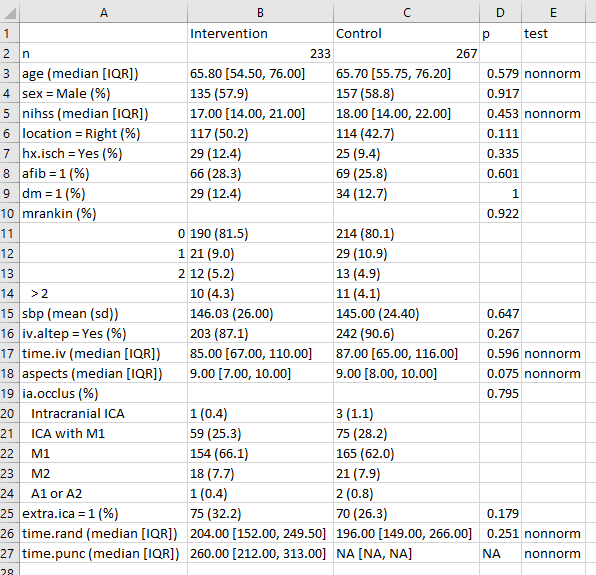
\includegraphics[width=0.9\linewidth]{images/fs-table1inExcel}

And from here, I can either drop it directly into Word, or present it as
is, or start tweaking it to meet formatting needs.

\subsection{Approach B: Produce the Table so you can cut and paste
it}\label{approach-b-produce-the-table-so-you-can-cut-and-paste-it}

\begin{Shaded}
\begin{Highlighting}[]
\KeywordTok{print}\NormalTok{(att2, }
      \DataTypeTok{nonnormal =} \KeywordTok{c}\NormalTok{(}\StringTok{"age"}\NormalTok{, }\StringTok{"nihss"}\NormalTok{, }\StringTok{"time.iv"}\NormalTok{, }\StringTok{"aspects"}\NormalTok{, }\StringTok{"time.rand"}\NormalTok{),}
      \DataTypeTok{exact =} \KeywordTok{c}\NormalTok{(}\StringTok{"location"}\NormalTok{, }\StringTok{"mrankin"}\NormalTok{),}
      \DataTypeTok{quote =} \OtherTok{TRUE}\NormalTok{, }\DataTypeTok{noSpaces =} \OtherTok{TRUE}\NormalTok{)}
\end{Highlighting}
\end{Shaded}

This will look like a mess by itself, but if you:

\begin{enumerate}
\def\labelenumi{\arabic{enumi}.}
\tightlist
\item
  copy and paste that mess into Excel
\item
  select Text to Columns from the Data menu
\item
  select Delimited, then Space and select Treat consecutive delimiters
  as one
\end{enumerate}

you should get something usable again.

Or, in Word,

\begin{enumerate}
\def\labelenumi{\arabic{enumi}.}
\tightlist
\item
  insert the text
\item
  select the text with your mouse
\item
  select Insert \ldots{} Table \ldots{} Convert Text to Table
\item
  place a quotation mark in the ``Other'' area under Separate text at
  \ldots{}
\end{enumerate}

After dropping blank columns, the result looks pretty good.

\section{A Controlled Biological Experiment - The Blood-Brain
Barrier}\label{a-controlled-biological-experiment---the-blood-brain-barrier}

My source for the data and the following explanatory paragraph is page
307 from \citet{RamseySchafer2002}. The original data come from
\citet{Barnett1995}.

\begin{quote}
The human brain (and that of rats, coincidentally) is protected from the
bacteria and toxins that course through the bloodstream by something
called the blood-brain barrier. After a method of disrupting the barrier
was developed, researchers tested this new mechanism, as follows. A
series of 34 rats were inoculated with human lung cancer cells to induce
brain tumors. After 9-11 days they were infused with either the barrier
disruption (BD) solution or, as a control, a normal saline (NS)
solution. Fifteen minutes later, the rats received a standard dose of a
particular therapeutic antibody (L6-F(ab')2. The key measure of the
effectiveness of transmission across the brain-blood barrier is the
ratio of the antibody concentration in the brain tumor to the antibody
concentration in normal tissue outside the brain. The rats were then
sacrificed, and the amounts of antibody in the brain tumor and in normal
tissue from the liver were measured. The study's primary objective is to
determine whether the antibody concentration in the tumor increased when
the blood-barrier disruption infusion was given, and if so, by how much?
\end{quote}

\section{\texorpdfstring{The \texttt{bloodbrain.csv}
file}{The bloodbrain.csv file}}\label{the-bloodbrain.csv-file}

Consider the data, available on the Data and Code page of
\href{https://github.com/THOMASELOVE/432-2018}{our course website} in
the \texttt{bloodbrain.csv} file, which includes the following
variables:

\begin{longtable}[]{@{}rl@{}}
\toprule
\begin{minipage}[b]{0.12\columnwidth}\raggedleft\strut
Variable\strut
\end{minipage} & \begin{minipage}[b]{0.59\columnwidth}\raggedright\strut
Description\strut
\end{minipage}\tabularnewline
\midrule
\endhead
\begin{minipage}[t]{0.12\columnwidth}\raggedleft\strut
\texttt{case}\strut
\end{minipage} & \begin{minipage}[t]{0.59\columnwidth}\raggedright\strut
identification number for the rat (1 - 34)\strut
\end{minipage}\tabularnewline
\begin{minipage}[t]{0.12\columnwidth}\raggedleft\strut
\texttt{brain}\strut
\end{minipage} & \begin{minipage}[t]{0.59\columnwidth}\raggedright\strut
an outcome: Brain tumor antibody count (per gram)\strut
\end{minipage}\tabularnewline
\begin{minipage}[t]{0.12\columnwidth}\raggedleft\strut
\texttt{liver}\strut
\end{minipage} & \begin{minipage}[t]{0.59\columnwidth}\raggedright\strut
an outcome: Liver antibody count (per gram)\strut
\end{minipage}\tabularnewline
\begin{minipage}[t]{0.12\columnwidth}\raggedleft\strut
\texttt{tlratio}\strut
\end{minipage} & \begin{minipage}[t]{0.59\columnwidth}\raggedright\strut
an outcome: tumor / liver concentration ratio\strut
\end{minipage}\tabularnewline
\begin{minipage}[t]{0.12\columnwidth}\raggedleft\strut
\texttt{solution}\strut
\end{minipage} & \begin{minipage}[t]{0.59\columnwidth}\raggedright\strut
the treatment: BD (barrier disruption) or NS (normal saline)\strut
\end{minipage}\tabularnewline
\begin{minipage}[t]{0.12\columnwidth}\raggedleft\strut
\texttt{sactime}\strut
\end{minipage} & \begin{minipage}[t]{0.59\columnwidth}\raggedright\strut
a design variable: Sacrifice time (hours; either 0.5, 3, 24 or 72)\strut
\end{minipage}\tabularnewline
\begin{minipage}[t]{0.12\columnwidth}\raggedleft\strut
\texttt{postin}\strut
\end{minipage} & \begin{minipage}[t]{0.59\columnwidth}\raggedright\strut
covariate: Days post-inoculation of lung cancer cells (9, 10 or
11)\strut
\end{minipage}\tabularnewline
\begin{minipage}[t]{0.12\columnwidth}\raggedleft\strut
\texttt{sex}\strut
\end{minipage} & \begin{minipage}[t]{0.59\columnwidth}\raggedright\strut
covariate: M or F\strut
\end{minipage}\tabularnewline
\begin{minipage}[t]{0.12\columnwidth}\raggedleft\strut
\texttt{wt.init}\strut
\end{minipage} & \begin{minipage}[t]{0.59\columnwidth}\raggedright\strut
covariate: Initial weight (grams)\strut
\end{minipage}\tabularnewline
\begin{minipage}[t]{0.12\columnwidth}\raggedleft\strut
\texttt{wt.loss}\strut
\end{minipage} & \begin{minipage}[t]{0.59\columnwidth}\raggedright\strut
covariate: Weight loss (grams)\strut
\end{minipage}\tabularnewline
\begin{minipage}[t]{0.12\columnwidth}\raggedleft\strut
\texttt{wt.tumor}\strut
\end{minipage} & \begin{minipage}[t]{0.59\columnwidth}\raggedright\strut
covariate: Tumor weight (10\textsuperscript{-4} grams)\strut
\end{minipage}\tabularnewline
\bottomrule
\end{longtable}

And here's what the data look like in R.

\begin{Shaded}
\begin{Highlighting}[]
\NormalTok{bloodbrain}
\end{Highlighting}
\end{Shaded}

\begin{verbatim}
# A tibble: 34 x 11
    case  brain   liver tlratio solution sactime postin sex   wt.init
   <int>  <int>   <int>   <dbl> <fct>      <dbl>  <int> <fct>   <int>
 1     1  41081 1456164  0.0282 BD         0.500     10 F         239
 2     2  44286 1602171  0.0276 BD         0.500     10 F         225
 3     3 102926 1601936  0.0642 BD         0.500     10 F         224
 4     4  25927 1776411  0.0146 BD         0.500     10 F         184
 5     5  42643 1351184  0.0316 BD         0.500     10 F         250
 6     6  31342 1790863  0.0175 NS         0.500     10 F         196
 7     7  22815 1633386  0.0140 NS         0.500     10 F         200
 8     8  16629 1618757  0.0103 NS         0.500     10 F         273
 9     9  22315 1567602  0.0142 NS         0.500     10 F         216
10    10  77961 1060057  0.0735 BD         3.00      10 F         267
# ... with 24 more rows, and 2 more variables: wt.loss <dbl>,
#   wt.tumor <int>
\end{verbatim}

\section{\texorpdfstring{A Table 1 for
\texttt{bloodbrain}}{A Table 1 for bloodbrain}}\label{a-table-1-for-bloodbrain}

\citet{Barnett1995} did not provide a Table 1 for these data, so let's
build one to compare the two \texttt{solutions} (\texttt{BD} vs.
\texttt{NS}) on the covariates and outcomes, plus the natural logarithm
of the tumor/liver concentration ratio (\texttt{tlratio}). We'll opt to
treat the sacrifice time (\texttt{sactime}) and the days
post-inoculation of lung cancer cells (\texttt{postin}) as categorical
rather than quantitative variables.

\begin{Shaded}
\begin{Highlighting}[]
\NormalTok{bloodbrain <-}\StringTok{ }\NormalTok{bloodbrain }\OperatorTok
\StringTok{    }\KeywordTok{mutate}\NormalTok{(}\DataTypeTok{logTL =} \KeywordTok{log}\NormalTok{(tlratio))}

\KeywordTok{dput}\NormalTok{(}\KeywordTok{names}\NormalTok{(bloodbrain))}
\end{Highlighting}
\end{Shaded}

\begin{verbatim}
c("case", "brain", "liver", "tlratio", "solution", "sactime", 
"postin", "sex", "wt.init", "wt.loss", "wt.tumor", "logTL")
\end{verbatim}

OK - there's the list of variables we'll need. I'll put the outcomes at
the bottom of the table.

\begin{Shaded}
\begin{Highlighting}[]
\NormalTok{bb.vars <-}\StringTok{ }\KeywordTok{c}\NormalTok{(}\StringTok{"sactime"}\NormalTok{, }\StringTok{"postin"}\NormalTok{, }\StringTok{"sex"}\NormalTok{, }\StringTok{"wt.init"}\NormalTok{, }\StringTok{"wt.loss"}\NormalTok{, }
             \StringTok{"wt.tumor"}\NormalTok{, }\StringTok{"brain"}\NormalTok{, }\StringTok{"liver"}\NormalTok{, }\StringTok{"tlratio"}\NormalTok{, }\StringTok{"logTL"}\NormalTok{)}

\NormalTok{bb.factors <-}\StringTok{ }\KeywordTok{c}\NormalTok{(}\StringTok{"sactime"}\NormalTok{, }\StringTok{"sex"}\NormalTok{, }\StringTok{"postin"}\NormalTok{)}

\NormalTok{bb.att1 <-}\StringTok{ }\KeywordTok{CreateTableOne}\NormalTok{(}\DataTypeTok{data =}\NormalTok{ bloodbrain,}
                          \DataTypeTok{vars =}\NormalTok{ bb.vars,}
                          \DataTypeTok{factorVars =}\NormalTok{ bb.factors,}
                          \DataTypeTok{strata =} \KeywordTok{c}\NormalTok{(}\StringTok{"solution"}\NormalTok{))}
\KeywordTok{summary}\NormalTok{(bb.att1)}
\end{Highlighting}
\end{Shaded}

\begin{verbatim}

     ### Summary of continuous variables ###

solution: BD
          n miss p.miss   mean    sd median    p25   p75    min   max
wt.init  17    0      0    243 3e+01  2e+02  2e+02 3e+02  2e+02 3e+02
wt.loss  17    0      0      3 5e+00  4e+00  1e+00 6e+00 -5e+00 1e+01
wt.tumor 17    0      0    157 8e+01  2e+02  1e+02 2e+02  2e+01 4e+02
brain    17    0      0  56043 3e+04  5e+04  4e+04 8e+04  6e+03 1e+05
liver    17    0      0 672577 7e+05  6e+05  2e+04 1e+06  2e+03 2e+06
tlratio  17    0      0      2 3e+00  1e-01  6e-02 3e+00  1e-02 9e+00
logTL    17    0      0     -1 2e+00 -2e+00 -3e+00 1e+00 -4e+00 2e+00
          skew kurt
wt.init  -0.39  0.7
wt.loss  -0.10  0.2
wt.tumor  0.53  1.0
brain     0.29 -0.6
liver     0.35 -1.7
tlratio   1.58  1.7
logTL     0.08 -1.7
-------------------------------------------------------- 
solution: NS
          n miss p.miss   mean    sd median    p25    p75    min   max
wt.init  17    0      0    240 3e+01  2e+02  2e+02  3e+02  2e+02 3e+02
wt.loss  17    0      0      4 4e+00  3e+00  2e+00  7e+00 -4e+00 1e+01
wt.tumor 17    0      0    209 1e+02  2e+02  2e+02  3e+02  3e+01 5e+02
brain    17    0      0  23887 1e+04  2e+04  1e+04  3e+04  1e+03 5e+04
liver    17    0      0 664975 7e+05  7e+05  2e+04  1e+06  9e+02 2e+06
tlratio  17    0      0      1 2e+00  5e-02  3e-02  9e-01  1e-02 7e+00
logTL    17    0      0     -2 2e+00 -3e+00 -3e+00 -7e-02 -5e+00 2e+00
          skew  kurt
wt.init   0.33 -0.48
wt.loss  -0.09  0.08
wt.tumor  0.63  0.77
brain     0.30 -0.35
liver     0.40 -1.56
tlratio   2.27  4.84
logTL     0.27 -1.61

p-values
             pNormal  pNonNormal
wt.init  0.807308940 0.641940278
wt.loss  0.683756156 0.876749808
wt.tumor 0.151510151 0.190482094
brain    0.001027678 0.002579901
liver    0.974853609 0.904045603
tlratio  0.320501715 0.221425879
logTL    0.351633525 0.221425879

Standardize mean differences
             1 vs 2
wt.init  0.08435244
wt.loss  0.14099823
wt.tumor 0.50397184
brain    1.23884159
liver    0.01089667
tlratio  0.34611465
logTL    0.32420504

=======================================================================================

     ### Summary of categorical variables ### 

solution: BD
     var  n miss p.miss level freq percent cum.percent
 sactime 17    0    0.0   0.5    5    29.4        29.4
                            3    4    23.5        52.9
                           24    4    23.5        76.5
                           72    4    23.5       100.0
                                                      
  postin 17    0    0.0     9    1     5.9         5.9
                           10   14    82.4        88.2
                           11    2    11.8       100.0
                                                      
     sex 17    0    0.0     F   13    76.5        76.5
                            M    4    23.5       100.0
                                                      
-------------------------------------------------------- 
solution: NS
     var  n miss p.miss level freq percent cum.percent
 sactime 17    0    0.0   0.5    4    23.5        23.5
                            3    5    29.4        52.9
                           24    4    23.5        76.5
                           72    4    23.5       100.0
                                                      
  postin 17    0    0.0     9    2    11.8        11.8
                           10   13    76.5        88.2
                           11    2    11.8       100.0
                                                      
     sex 17    0    0.0     F   13    76.5        76.5
                            M    4    23.5       100.0
                                                      

p-values
          pApprox pExact
sactime 0.9739246      1
postin  0.8309504      1
sex     1.0000000      1

Standardize mean differences
           1 vs 2
sactime 0.1622214
postin  0.2098877
sex     0.0000000
\end{verbatim}

Note that, in this particular case, the decisions we make about
normality vs.~non-normality (for quantitative variables) and the
decisions we make about approximate vs.~exact testing (for categorical
variables) won't actually change the implications of the \emph{p}
values. Each approach gives similar results for each variable. Of
course, that's not always true.

\subsection{\texorpdfstring{Generate final Table 1 for
\texttt{bloodbrain}}{Generate final Table 1 for bloodbrain}}\label{generate-final-table-1-for-bloodbrain}

I'll choose to treat \texttt{tlratio} and its logarithm as non-Normal,
but otherwise, use t tests, but admittedly, that's an arbitrary
decision, really.

\begin{Shaded}
\begin{Highlighting}[]
\KeywordTok{print}\NormalTok{(bb.att1, }\DataTypeTok{nonnormal =} \KeywordTok{c}\NormalTok{(}\StringTok{"tlratio"}\NormalTok{, }\StringTok{"logTL"}\NormalTok{))}
\end{Highlighting}
\end{Shaded}

\begin{verbatim}
                        Stratified by solution
                         BD                      NS                      
  n                             17                      17               
  sactime (%)                                                            
     0.5                         5 (29.4)                4 (23.5)        
     3                           4 (23.5)                5 (29.4)        
     24                          4 (23.5)                4 (23.5)        
     72                          4 (23.5)                4 (23.5)        
  postin (%)                                                             
     9                           1 ( 5.9)                2 (11.8)        
     10                         14 (82.4)               13 (76.5)        
     11                          2 (11.8)                2 (11.8)        
  sex = M (%)                    4 (23.5)                4 (23.5)        
  wt.init (mean (sd))       242.82 (27.23)          240.47 (28.54)       
  wt.loss (mean (sd))         3.34 (4.68)             3.94 (3.88)        
  wt.tumor (mean (sd))      157.29 (84.00)          208.53 (116.68)      
  brain (mean (sd))       56043.41 (33675.40)     23887.18 (14610.53)    
  liver (mean (sd))      672577.35 (694479.58)   664975.47 (700773.13)   
  tlratio (median [IQR])      0.12 [0.06, 2.84]       0.05 [0.03, 0.94]  
  logTL (median [IQR])       -2.10 [-2.74, 1.04]     -2.95 [-3.41, -0.07]
                        Stratified by solution
                         p      test   
  n                                    
  sactime (%)             0.974        
     0.5                               
     3                                 
     24                                
     72                                
  postin (%)              0.831        
     9                                 
     10                                
     11                                
  sex = M (%)             1.000        
  wt.init (mean (sd))     0.807        
  wt.loss (mean (sd))     0.684        
  wt.tumor (mean (sd))    0.152        
  brain (mean (sd))       0.001        
  liver (mean (sd))       0.975        
  tlratio (median [IQR])  0.221 nonnorm
  logTL (median [IQR])    0.221 nonnorm
\end{verbatim}

Or, we can get an Excel-readable version placed in a \texttt{data}
subfolder, using

\begin{Shaded}
\begin{Highlighting}[]
\NormalTok{bb.t1 <-}\StringTok{ }\KeywordTok{print}\NormalTok{(bb.att1, }\DataTypeTok{nonnormal =} \KeywordTok{c}\NormalTok{(}\StringTok{"tlratio"}\NormalTok{, }\StringTok{"logTL"}\NormalTok{), }\DataTypeTok{quote =} \OtherTok{FALSE}\NormalTok{,}
               \DataTypeTok{noSpaces =} \OtherTok{TRUE}\NormalTok{, }\DataTypeTok{printToggle =} \OtherTok{FALSE}\NormalTok{)}

\KeywordTok{write.csv}\NormalTok{(bb.t1, }\DataTypeTok{file =} \StringTok{"data/bb-table1.csv"}\NormalTok{)}
\end{Highlighting}
\end{Shaded}

which, when dropped into Excel, will look like this:

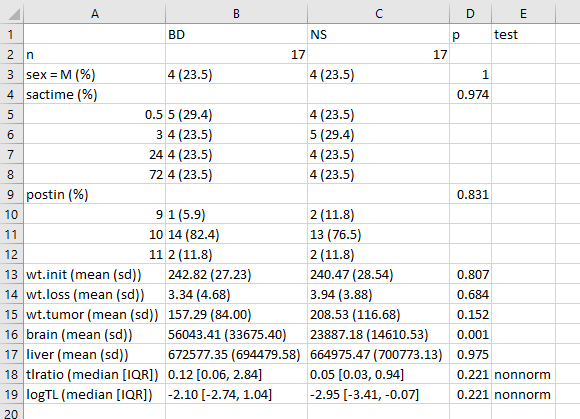
\includegraphics[width=0.9\linewidth]{images/bb-table1inExcel}

One thing I would definitely clean up here, in practice, is to change
the presentation of the \emph{p} value for \texttt{sex} from 1 to
\textgreater{} 0.99, or just omit it altogether. I'd also drop the
\texttt{computer-ese} where possible, add units for the measures, round
\textbf{a lot}, identify the outcomes carefully, and use notes to
indicate deviations from the main approach.

\subsection{A More Finished Version (after Cleanup in
Word)}\label{a-more-finished-version-after-cleanup-in-word}

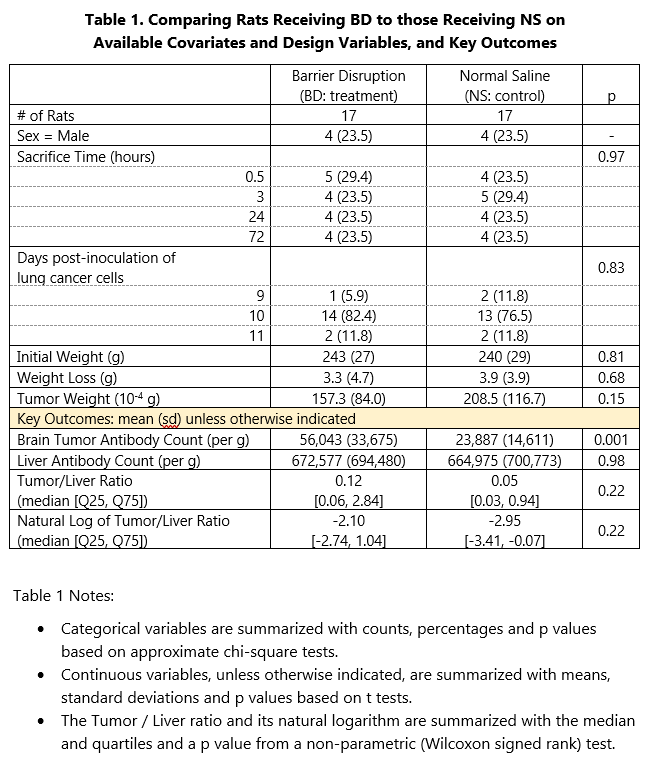
\includegraphics[width=0.95\linewidth]{images/bb-table1inWord}

\chapter{Linear Regression on a small SMART data
set}\label{linear-regression-on-a-small-smart-data-set}

\section{BRFSS and SMART}\label{brfss-and-smart}

The Centers for Disease Control analyzes Behavioral Risk Factor
Surveillance System (BRFSS) survey data for specific metropolitan and
micropolitan statistical areas (MMSAs) in a program called the
\href{https://www.cdc.gov/brfss/smart/Smart_data.htm}{Selected
Metropolitan/Micropolitan Area Risk Trends of BRFSS} (SMART BRFSS.)

In this work, we will focus on
\href{https://www.cdc.gov/brfss/smart/smart_2016.html}{data from the
2016 SMART}, and in particular on data from the Cleveland-Elyria, OH,
Metropolitan Statistical Area. The purpose of this survey is to provide
localized health information that can help public health practitioners
identify local emerging health problems, plan and evaluate local
responses, and efficiently allocate resources to specific needs.

\subsection{Key resources}\label{key-resources}

\begin{itemize}
\tightlist
\item
  the full data are available in the form of the 2016 SMART BRFSS MMSA
  Data, found in a zipped
  \href{https://www.cdc.gov/brfss/smart/2016/MMSA2016_XPT.zip}{SAS
  Transport Format} file. The data were released in August 2017.
\item
  the
  \href{https://www.cdc.gov/brfss/smart/2016/mmsa_varlayout_16.pdf}{MMSA
  Variable Layout PDF} which simply lists the variables included in the
  data file
\item
  the
  \href{https://www.cdc.gov/brfss/annual_data/2016/pdf/2016_calculated_variables_version4.pdf}{Calculated
  Variables PDF} which describes the risk factors by data variable names
  - there is also an
  \href{https://www.cdc.gov/brfss/annual_data/2016/Summary_Matrix_16.html}{online
  summary matrix of these calculated variables}, as well.
\item
  the lengthy
  \href{https://www.cdc.gov/brfss/questionnaires/pdf-ques/2016_BRFSS_Questionnaire_FINAL.pdf}{2016
  Survey Questions PDF} which lists all questions asked as part of the
  BRFSS in 2016
\item
  the enormous
  \href{https://www.cdc.gov/brfss/annual_data/2016/pdf/codebook16_llcp.pdf}{Codebook
  for the 2016 BRFSS Survey PDF} which identifies the variables by name
  for us.
\end{itemize}

Later this term, we'll use all of those resources to help construct a
more complete data set than we'll study today. I'll also demonstrate how
I built the \texttt{smartcle1} data set that we'll use in this Chapter.

\section{\texorpdfstring{The \texttt{smartcle1} data:
Cookbook}{The smartcle1 data: Cookbook}}\label{the-smartcle1-data-cookbook}

The \texttt{smartcle1.csv} data file available on the Data and Code page
of \href{https://github.com/THOMASELOVE/432-2018}{our website} describes
information on 11 variables for 1036 respondents to the BRFSS 2016, who
live in the Cleveland-Elyria, OH, Metropolitan Statistical Area. The
variables in the \texttt{smartcle1.csv} file are listed below, along
with (in some cases) the BRFSS items that generate these responses.

\begin{longtable}[]{@{}rl@{}}
\toprule
\begin{minipage}[b]{0.14\columnwidth}\raggedleft\strut
Variable\strut
\end{minipage} & \begin{minipage}[b]{0.74\columnwidth}\raggedright\strut
Description\strut
\end{minipage}\tabularnewline
\midrule
\endhead
\begin{minipage}[t]{0.14\columnwidth}\raggedleft\strut
\texttt{SEQNO}\strut
\end{minipage} & \begin{minipage}[t]{0.74\columnwidth}\raggedright\strut
respondent identification number (all begin with 2016)\strut
\end{minipage}\tabularnewline
\begin{minipage}[t]{0.14\columnwidth}\raggedleft\strut
\texttt{physhealth}\strut
\end{minipage} & \begin{minipage}[t]{0.74\columnwidth}\raggedright\strut
Now thinking about your physical health, which includes physical illness
and injury, for how many days during the past 30 days was your physical
health not good?\strut
\end{minipage}\tabularnewline
\begin{minipage}[t]{0.14\columnwidth}\raggedleft\strut
\texttt{menthealth}\strut
\end{minipage} & \begin{minipage}[t]{0.74\columnwidth}\raggedright\strut
Now thinking about your mental health, which includes stress,
depression, and problems with emotions, for how many days during the
past 30 days was your mental health not good?\strut
\end{minipage}\tabularnewline
\begin{minipage}[t]{0.14\columnwidth}\raggedleft\strut
\texttt{poorhealth}\strut
\end{minipage} & \begin{minipage}[t]{0.74\columnwidth}\raggedright\strut
During the past 30 days, for about how many days did poor physical or
mental health keep you from doing your usual activities, such as
self-care, work, or recreation?\strut
\end{minipage}\tabularnewline
\begin{minipage}[t]{0.14\columnwidth}\raggedleft\strut
\texttt{genhealth}\strut
\end{minipage} & \begin{minipage}[t]{0.74\columnwidth}\raggedright\strut
Would you say that in general, your health is \ldots{} (five categories:
Excellent, Very Good, Good, Fair or Poor)\strut
\end{minipage}\tabularnewline
\begin{minipage}[t]{0.14\columnwidth}\raggedleft\strut
\texttt{bmi}\strut
\end{minipage} & \begin{minipage}[t]{0.74\columnwidth}\raggedright\strut
Body mass index, in kg/m\textsuperscript{2}\strut
\end{minipage}\tabularnewline
\begin{minipage}[t]{0.14\columnwidth}\raggedleft\strut
\texttt{female}\strut
\end{minipage} & \begin{minipage}[t]{0.74\columnwidth}\raggedright\strut
Sex, 1 = female, 0 = male\strut
\end{minipage}\tabularnewline
\begin{minipage}[t]{0.14\columnwidth}\raggedleft\strut
\texttt{internet30}\strut
\end{minipage} & \begin{minipage}[t]{0.74\columnwidth}\raggedright\strut
Have you used the internet in the past 30 days? (1 = yes, 0 = no)\strut
\end{minipage}\tabularnewline
\begin{minipage}[t]{0.14\columnwidth}\raggedleft\strut
\texttt{exerany}\strut
\end{minipage} & \begin{minipage}[t]{0.74\columnwidth}\raggedright\strut
During the past month, other than your regular job, did you participate
in any physical activities or exercises such as running, calisthenics,
golf, gardening, or walking for exercise? (1 = yes, 0 = no)\strut
\end{minipage}\tabularnewline
\begin{minipage}[t]{0.14\columnwidth}\raggedleft\strut
\texttt{sleephrs}\strut
\end{minipage} & \begin{minipage}[t]{0.74\columnwidth}\raggedright\strut
On average, how many hours of sleep do you get in a 24-hour
period?\strut
\end{minipage}\tabularnewline
\begin{minipage}[t]{0.14\columnwidth}\raggedleft\strut
\texttt{alcdays}\strut
\end{minipage} & \begin{minipage}[t]{0.74\columnwidth}\raggedright\strut
How many days during the past 30 days did you have at least one drink of
any alcoholic beverage such as beer, wine, a malt beverage or
liquor?\strut
\end{minipage}\tabularnewline
\bottomrule
\end{longtable}

\begin{Shaded}
\begin{Highlighting}[]
\KeywordTok{str}\NormalTok{(smartcle1)}
\end{Highlighting}
\end{Shaded}

\begin{verbatim}
Classes 'tbl_df', 'tbl' and 'data.frame':   1036 obs. of  11 variables:
 $ SEQNO     : num  2.02e+09 2.02e+09 2.02e+09 2.02e+09 2.02e+09 ...
 $ physhealth: int  0 0 1 0 5 4 2 2 0 0 ...
 $ menthealth: int  0 0 5 0 0 18 0 3 0 0 ...
 $ poorhealth: int  NA NA 0 NA 0 6 0 0 NA NA ...
 $ genhealth : Factor w/ 5 levels "1_Excellent",..: 2 1 2 3 1 2 3 3 2 3 ...
 $ bmi       : num  26.7 23.7 26.9 21.7 24.1 ...
 $ female    : int  1 0 0 1 0 0 1 1 0 0 ...
 $ internet30: int  1 1 1 1 1 1 1 1 1 1 ...
 $ exerany   : int  1 1 0 1 1 1 1 1 1 0 ...
 $ sleephrs  : int  6 6 8 9 7 5 9 7 7 7 ...
 $ alcdays   : int  1 4 4 3 2 28 4 2 4 25 ...
\end{verbatim}

\section{\texorpdfstring{\texttt{smartcle2}: Omitting Missing
Observations: Complete-Case
Analyses}{smartcle2: Omitting Missing Observations: Complete-Case Analyses}}\label{smartcle2-omitting-missing-observations-complete-case-analyses}

For the purpose of fitting our first few models, we will eliminate the
missingness problem, and look only at the \emph{complete cases} in our
\texttt{smartcle1} data. We will discuss methods for imputing missing
data later in these Notes.

To inspect the missingness in our data, we might consider using the
\texttt{skim} function from the \texttt{skimr} package. We'll exclude
the respondent identifier code (\texttt{SEQNO}) from this summary as
uninteresting.

\begin{Shaded}
\begin{Highlighting}[]
\KeywordTok{skim_with}\NormalTok{(}\DataTypeTok{numeric =} \KeywordTok{list}\NormalTok{(}\DataTypeTok{hist =} \OtherTok{NULL}\NormalTok{), }\DataTypeTok{integer =} \KeywordTok{list}\NormalTok{(}\DataTypeTok{hist =} \OtherTok{NULL}\NormalTok{))}
\NormalTok{## above line eliminates the sparkline histograms}
\NormalTok{## it can be commented out when working in the console,}
\NormalTok{## but I need it to produce the Notes without errors right now}

\NormalTok{smartcle1 }\OperatorTok\StringTok{ }
\StringTok{    }\KeywordTok{skim}\NormalTok{(}\OperatorTok{-}\NormalTok{SEQNO)}
\end{Highlighting}
\end{Shaded}

\begin{verbatim}
Skim summary statistics
 n obs: 1036 
 n variables: 11 

Variable type: factor 
  variable missing complete    n n_unique
 genhealth       3     1033 1036        5
                             top_counts ordered
 2_V: 350, 3_G: 344, 1_E: 173, 4_F: 122   FALSE

Variable type: integer 
   variable missing complete    n mean   sd p0 p25 median p75 p100
    alcdays      46      990 1036 4.65 8.05  0   0      1   4   30
    exerany       3     1033 1036 0.76 0.43  0   1      1   1    1
     female       0     1036 1036 0.6  0.49  0   0      1   1    1
 internet30       6     1030 1036 0.81 0.39  0   1      1   1    1
 menthealth      11     1025 1036 2.72 6.82  0   0      0   2   30
 physhealth      17     1019 1036 3.97 8.67  0   0      0   2   30
 poorhealth     543      493 1036 4.07 8.09  0   0      0   3   30
   sleephrs       8     1028 1036 7.02 1.53  1   6      7   8   20

Variable type: numeric 
 variable missing complete    n  mean   sd    p0  p25 median   p75  p100
      bmi      84      952 1036 27.89 6.47 12.71 23.7  26.68 30.53 66.06
\end{verbatim}

Now, we'll create a new tibble called \texttt{smartcle2} which contains
every variable except \texttt{poorhealth}, and which includes all
respondents with complete data on the variables (other than
\texttt{poorhealth}). We'll store those observations with complete data
in the \texttt{smartcle2} tibble.

\begin{Shaded}
\begin{Highlighting}[]
\NormalTok{smartcle2 <-}\StringTok{ }\NormalTok{smartcle1 }\OperatorTok\StringTok{ }
\StringTok{    }\KeywordTok{select}\NormalTok{(}\OperatorTok{-}\NormalTok{poorhealth) }\OperatorTok
\StringTok{    }\KeywordTok{filter}\NormalTok{(}\KeywordTok{complete.cases}\NormalTok{(.))}

\NormalTok{smartcle2}
\end{Highlighting}
\end{Shaded}

\begin{verbatim}
# A tibble: 896 x 10
     SEQNO physhealth menthealth genhealth   bmi female internet30 exerany
     <dbl>      <int>      <int> <fct>     <dbl>  <int>      <int>   <int>
 1  2.02e9          0          0 2_VeryGo~  26.7      1          1       1
 2  2.02e9          0          0 1_Excell~  23.7      0          1       1
 3  2.02e9          1          5 2_VeryGo~  26.9      0          1       0
 4  2.02e9          0          0 3_Good     21.7      1          1       1
 5  2.02e9          5          0 1_Excell~  24.1      0          1       1
 6  2.02e9          4         18 2_VeryGo~  27.6      0          1       1
 7  2.02e9          2          0 3_Good     25.7      1          1       1
 8  2.02e9          2          3 3_Good     28.5      1          1       1
 9  2.02e9          0          0 2_VeryGo~  28.6      0          1       1
10  2.02e9          0          0 3_Good     23.1      0          1       0
# ... with 886 more rows, and 2 more variables: sleephrs <int>,
#   alcdays <int>
\end{verbatim}

Note that there are only 896 respondents with \textbf{complete} data on
the 10 variables (excluding \texttt{poorhealth}) in the
\texttt{smartcle2} tibble, as compared to our original
\texttt{smartcle1} data which described 1036 respondents and 11
variables, but with lots of missing data.

\section{\texorpdfstring{Summarizing the \texttt{smartcle2} data
numerically}{Summarizing the smartcle2 data numerically}}\label{summarizing-the-smartcle2-data-numerically}

\subsection{\texorpdfstring{The New Toy: The \texttt{skim}
function}{The New Toy: The skim function}}\label{the-new-toy-the-skim-function}

\begin{Shaded}
\begin{Highlighting}[]
\KeywordTok{skim}\NormalTok{(smartcle2, }\OperatorTok{-}\NormalTok{SEQNO)}
\end{Highlighting}
\end{Shaded}

\begin{verbatim}
Skim summary statistics
 n obs: 896 
 n variables: 10 

Variable type: factor 
  variable missing complete   n n_unique
 genhealth       0      896 896        5
                             top_counts ordered
 2_V: 306, 3_G: 295, 1_E: 155, 4_F: 102   FALSE

Variable type: integer 
   variable missing complete   n mean   sd p0 p25 median p75 p100
    alcdays       0      896 896 4.83 8.14  0   0      1   5   30
    exerany       0      896 896 0.77 0.42  0   1      1   1    1
     female       0      896 896 0.58 0.49  0   0      1   1    1
 internet30       0      896 896 0.81 0.39  0   1      1   1    1
 menthealth       0      896 896 2.69 6.72  0   0      0   2   30
 physhealth       0      896 896 3.99 8.64  0   0      0   2   30
   sleephrs       0      896 896 7.02 1.48  1   6      7   8   20

Variable type: numeric 
 variable missing complete   n  mean   sd    p0  p25 median   p75  p100
      bmi       0      896 896 27.87 6.33 12.71 23.7   26.8 30.53 66.06
\end{verbatim}

\subsection{\texorpdfstring{The usual \texttt{summary} for a data
frame}{The usual summary for a data frame}}\label{the-usual-summary-for-a-data-frame}

Of course, we can use the usual \texttt{summary} to get some basic
information about the data.

\begin{Shaded}
\begin{Highlighting}[]
\KeywordTok{summary}\NormalTok{(smartcle2)}
\end{Highlighting}
\end{Shaded}

\begin{verbatim}
     SEQNO             physhealth      menthealth           genhealth  
 Min.   :2.016e+09   Min.   : 0.00   Min.   : 0.000   1_Excellent:155  
 1st Qu.:2.016e+09   1st Qu.: 0.00   1st Qu.: 0.000   2_VeryGood :306  
 Median :2.016e+09   Median : 0.00   Median : 0.000   3_Good     :295  
 Mean   :2.016e+09   Mean   : 3.99   Mean   : 2.693   4_Fair     :102  
 3rd Qu.:2.016e+09   3rd Qu.: 2.00   3rd Qu.: 2.000   5_Poor     : 38  
 Max.   :2.016e+09   Max.   :30.00   Max.   :30.000                    
      bmi            female         internet30        exerany      
 Min.   :12.71   Min.   :0.0000   Min.   :0.0000   Min.   :0.0000  
 1st Qu.:23.70   1st Qu.:0.0000   1st Qu.:1.0000   1st Qu.:1.0000  
 Median :26.80   Median :1.0000   Median :1.0000   Median :1.0000  
 Mean   :27.87   Mean   :0.5848   Mean   :0.8147   Mean   :0.7667  
 3rd Qu.:30.53   3rd Qu.:1.0000   3rd Qu.:1.0000   3rd Qu.:1.0000  
 Max.   :66.06   Max.   :1.0000   Max.   :1.0000   Max.   :1.0000  
    sleephrs         alcdays      
 Min.   : 1.000   Min.   : 0.000  
 1st Qu.: 6.000   1st Qu.: 0.000  
 Median : 7.000   Median : 1.000  
 Mean   : 7.022   Mean   : 4.834  
 3rd Qu.: 8.000   3rd Qu.: 5.000  
 Max.   :20.000   Max.   :30.000  
\end{verbatim}

\subsection{\texorpdfstring{The \texttt{describe} function in
\texttt{Hmisc}}{The describe function in Hmisc}}\label{the-describe-function-in-hmisc}

Or we can use the \texttt{describe} function from the \texttt{Hmisc}
package.

\begin{Shaded}
\begin{Highlighting}[]
\NormalTok{Hmisc}\OperatorTok{::}\KeywordTok{describe}\NormalTok{(}\KeywordTok{select}\NormalTok{(smartcle2, bmi, genhealth, female))}
\end{Highlighting}
\end{Shaded}

\begin{verbatim}
select(smartcle2, bmi, genhealth, female) 

 3  Variables      896  Observations
---------------------------------------------------------------------------
bmi 
       n  missing distinct     Info     Mean      Gmd      .05      .10 
     896        0      467        1    27.87    6.572    20.06    21.23 
     .25      .50      .75      .90      .95 
   23.70    26.80    30.53    35.36    39.30 

lowest : 12.71 13.34 14.72 16.22 17.30, highest: 56.89 57.04 60.95 61.84 66.06
---------------------------------------------------------------------------
genhealth 
       n  missing distinct 
     896        0        5 
                                                                      
Value      1_Excellent  2_VeryGood      3_Good      4_Fair      5_Poor
Frequency          155         306         295         102          38
Proportion       0.173       0.342       0.329       0.114       0.042
---------------------------------------------------------------------------
female 
       n  missing distinct     Info      Sum     Mean      Gmd 
     896        0        2    0.728      524   0.5848   0.4862 

---------------------------------------------------------------------------
\end{verbatim}

\section{Counting as exploratory data
analysis}\label{counting-as-exploratory-data-analysis}

Counting things can be amazingly useful.

\subsection{How many respondents had exercised in the past 30 days? Did
this vary by
sex?}\label{how-many-respondents-had-exercised-in-the-past-30-days-did-this-vary-by-sex}

\begin{Shaded}
\begin{Highlighting}[]
\NormalTok{smartcle2 }\OperatorTok\StringTok{ }\KeywordTok{count}\NormalTok{(female, exerany) }\OperatorTok\StringTok{ }\KeywordTok{mutate}\NormalTok{(}\DataTypeTok{percent =} \DecValTok{100}\OperatorTok{*}\NormalTok{n }\OperatorTok{/}\StringTok{ }\KeywordTok{sum}\NormalTok{(n))}
\end{Highlighting}
\end{Shaded}

\begin{verbatim}
# A tibble: 4 x 4
  female exerany     n percent
   <int>   <int> <int>   <dbl>
1      0       0    64    7.14
2      0       1   308   34.4 
3      1       0   145   16.2 
4      1       1   379   42.3 
\end{verbatim}

so we know now that 42.3\% of the subjects in our data were women who
exercised. Suppose that instead we want to find the percentage of
exercisers within each sex\ldots{}

\begin{Shaded}
\begin{Highlighting}[]
\NormalTok{smartcle2 }\OperatorTok
\StringTok{    }\KeywordTok{count}\NormalTok{(female, exerany) }\OperatorTok
\StringTok{    }\KeywordTok{group_by}\NormalTok{(female) }\OperatorTok
\StringTok{    }\KeywordTok{mutate}\NormalTok{(}\DataTypeTok{prob =} \DecValTok{100}\OperatorTok{*}\NormalTok{n }\OperatorTok{/}\StringTok{ }\KeywordTok{sum}\NormalTok{(n)) }
\end{Highlighting}
\end{Shaded}

\begin{verbatim}
# A tibble: 4 x 4
# Groups:   female [2]
  female exerany     n  prob
   <int>   <int> <int> <dbl>
1      0       0    64  17.2
2      0       1   308  82.8
3      1       0   145  27.7
4      1       1   379  72.3
\end{verbatim}

and now we know that 82.8\% of the males exercised at least once in the
last 30 days, as compared to 72.3\% of the females.

\subsection{\texorpdfstring{What's the distribution of
\texttt{sleephrs}?}{What's the distribution of sleephrs?}}\label{whats-the-distribution-of-sleephrs}

We can count quantitative variables with discrete sets of possible
values, like \texttt{sleephrs}, which is captured as an integer (that
must fall between 0 and 24.)

\begin{Shaded}
\begin{Highlighting}[]
\NormalTok{smartcle2 }\OperatorTok\StringTok{ }\KeywordTok{count}\NormalTok{(sleephrs)}
\end{Highlighting}
\end{Shaded}

\begin{verbatim}
# A tibble: 14 x 2
   sleephrs     n
      <int> <int>
 1        1     5
 2        2     1
 3        3     6
 4        4    20
 5        5    63
 6        6   192
 7        7   276
 8        8   266
 9        9    38
10       10    22
11       11     2
12       12     2
13       16     2
14       20     1
\end{verbatim}

Of course, a natural summary of a quantitative variable like this would
be graphical.

\begin{Shaded}
\begin{Highlighting}[]
\KeywordTok{ggplot}\NormalTok{(smartcle2, }\KeywordTok{aes}\NormalTok{(sleephrs)) }\OperatorTok{+}
\StringTok{    }\KeywordTok{geom_histogram}\NormalTok{(}\DataTypeTok{binwidth =} \DecValTok{1}\NormalTok{, }\DataTypeTok{fill =} \StringTok{"dodgerblue"}\NormalTok{, }\DataTypeTok{col =} \StringTok{"darkred"}\NormalTok{)}
\end{Highlighting}
\end{Shaded}

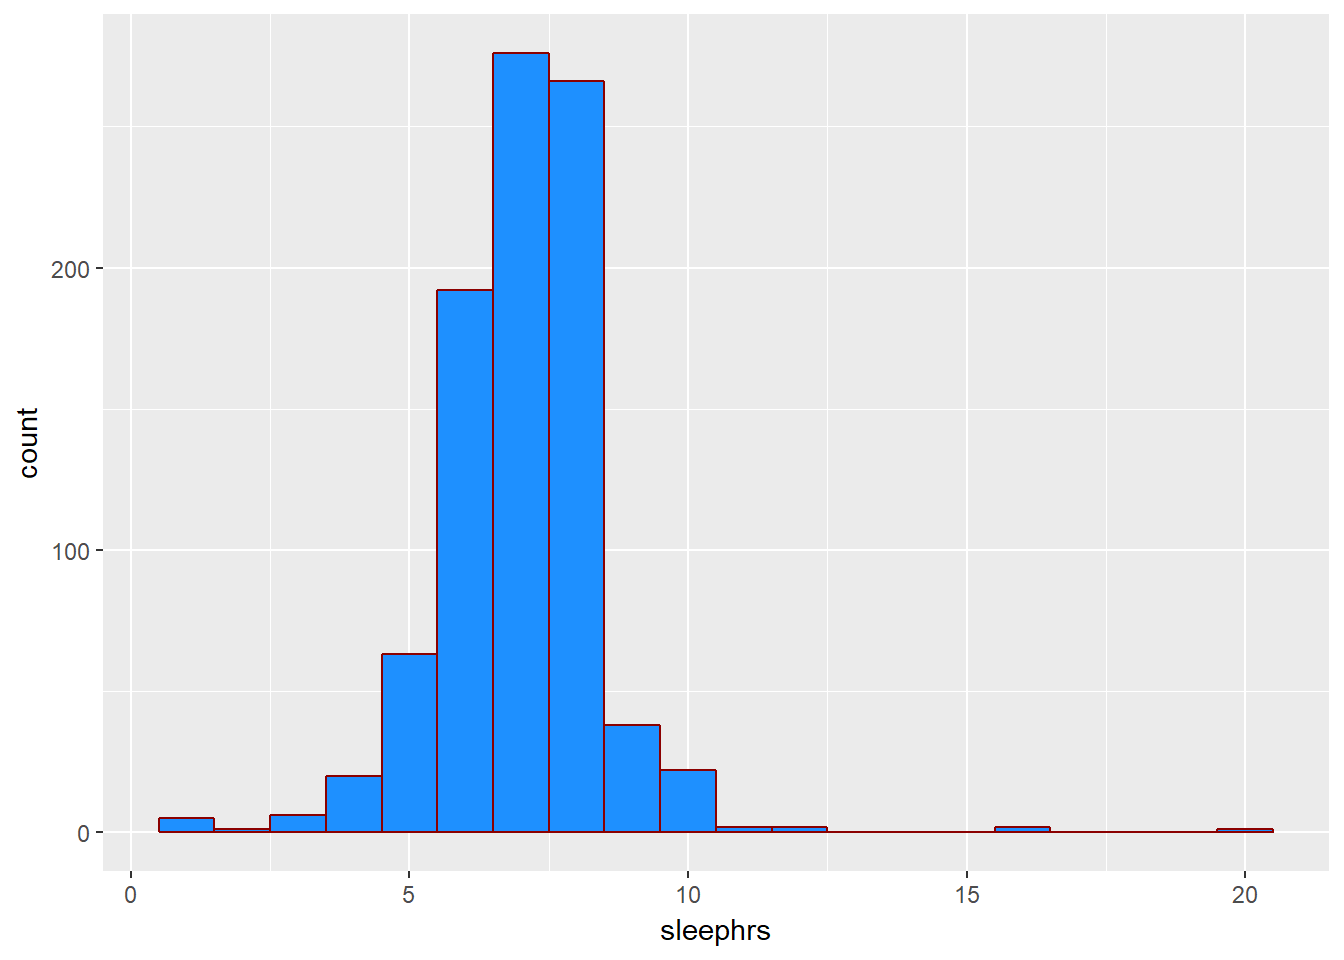
\includegraphics{bookdown-demo_files/figure-latex/c2_histogram_sleephrs_smartcle2-1.pdf}

\subsection{\texorpdfstring{What's the distribution of
\texttt{BMI}?}{What's the distribution of BMI?}}\label{whats-the-distribution-of-bmi}

\begin{Shaded}
\begin{Highlighting}[]
\KeywordTok{ggplot}\NormalTok{(smartcle2, }\KeywordTok{aes}\NormalTok{(bmi)) }\OperatorTok{+}
\StringTok{    }\KeywordTok{geom_histogram}\NormalTok{(}\DataTypeTok{bins =} \DecValTok{30}\NormalTok{, }\DataTypeTok{col =} \StringTok{"white"}\NormalTok{)}
\end{Highlighting}
\end{Shaded}

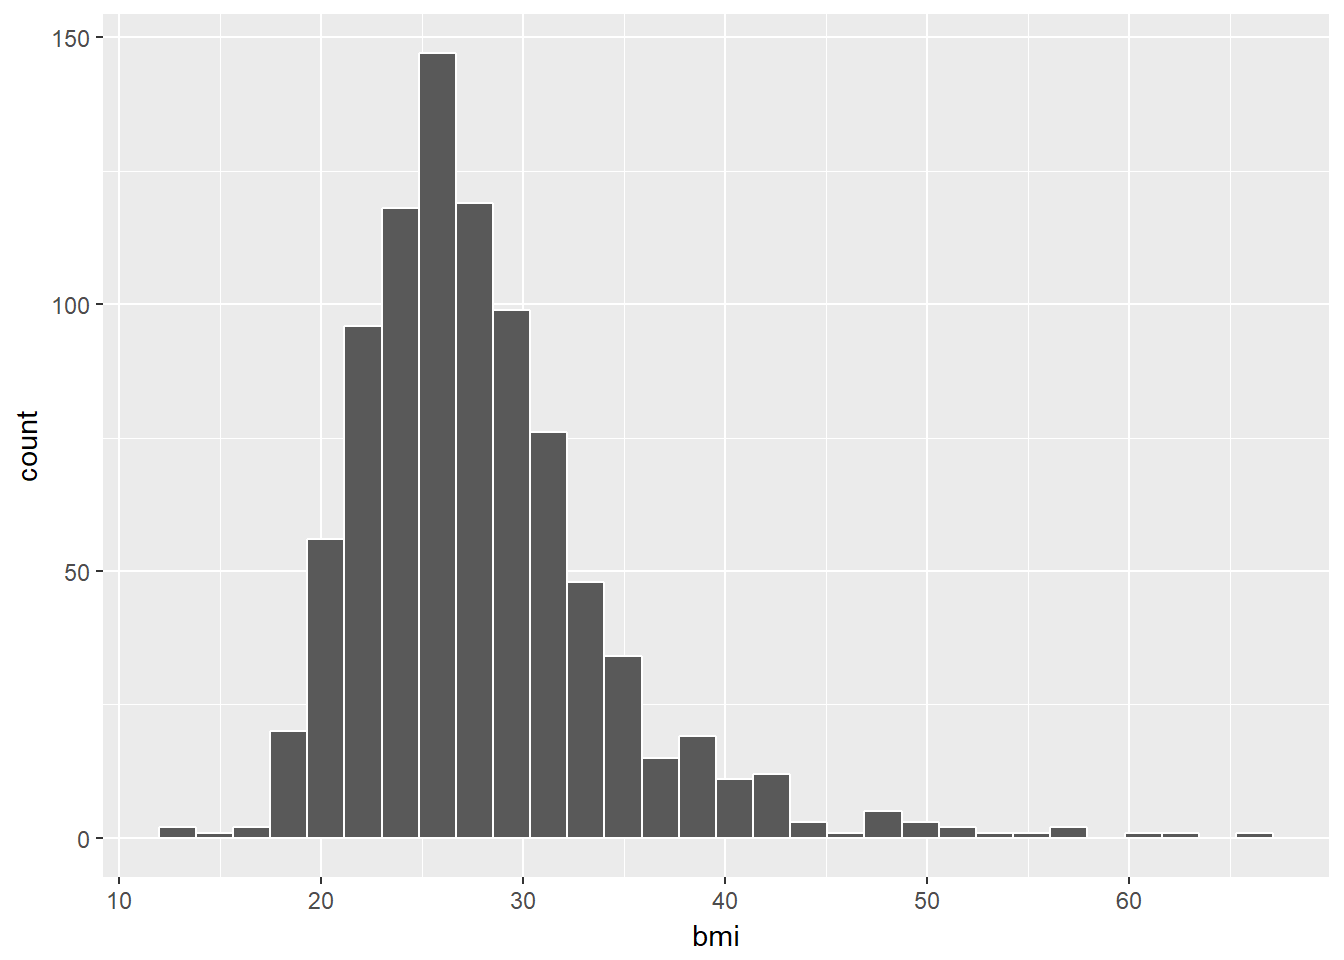
\includegraphics{bookdown-demo_files/figure-latex/c2_histogram_bmi_smartcle2-1.pdf}

\subsection{How many of the respondents have a BMI below
30?}\label{how-many-of-the-respondents-have-a-bmi-below-30}

\begin{Shaded}
\begin{Highlighting}[]
\NormalTok{smartcle2 }\OperatorTok\StringTok{ }\KeywordTok{count}\NormalTok{(bmi }\OperatorTok{<}\StringTok{ }\DecValTok{30}\NormalTok{) }\OperatorTok\StringTok{ }\KeywordTok{mutate}\NormalTok{(}\DataTypeTok{proportion =}\NormalTok{ n }\OperatorTok{/}\StringTok{ }\KeywordTok{sum}\NormalTok{(n))}
\end{Highlighting}
\end{Shaded}

\begin{verbatim}
# A tibble: 2 x 3
  `bmi < 30`     n proportion
  <lgl>      <int>      <dbl>
1 F            253      0.282
2 T            643      0.718
\end{verbatim}

\subsection{How many of the respondents who have a BMI \textless{} 30
exercised?}\label{how-many-of-the-respondents-who-have-a-bmi-30-exercised}

\begin{Shaded}
\begin{Highlighting}[]
\NormalTok{smartcle2 }\OperatorTok\StringTok{ }\KeywordTok{count}\NormalTok{(exerany, bmi }\OperatorTok{<}\StringTok{ }\DecValTok{30}\NormalTok{) }\OperatorTok
\StringTok{    }\KeywordTok{group_by}\NormalTok{(exerany) }\OperatorTok
\StringTok{    }\KeywordTok{mutate}\NormalTok{(}\DataTypeTok{percent =} \DecValTok{100}\OperatorTok{*}\NormalTok{n}\OperatorTok{/}\KeywordTok{sum}\NormalTok{(n))}
\end{Highlighting}
\end{Shaded}

\begin{verbatim}
# A tibble: 4 x 4
# Groups:   exerany [2]
  exerany `bmi < 30`     n percent
    <int> <lgl>      <int>   <dbl>
1       0 F             88    42.1
2       0 T            121    57.9
3       1 F            165    24.0
4       1 T            522    76.0
\end{verbatim}

\subsection{Is obesity associated with sex, in these
data?}\label{is-obesity-associated-with-sex-in-these-data}

\begin{Shaded}
\begin{Highlighting}[]
\NormalTok{smartcle2 }\OperatorTok\StringTok{ }\KeywordTok{count}\NormalTok{(female, bmi }\OperatorTok{<}\StringTok{ }\DecValTok{30}\NormalTok{) }\OperatorTok
\StringTok{    }\KeywordTok{group_by}\NormalTok{(female) }\OperatorTok
\StringTok{    }\KeywordTok{mutate}\NormalTok{(}\DataTypeTok{percent =} \DecValTok{100}\OperatorTok{*}\NormalTok{n}\OperatorTok{/}\KeywordTok{sum}\NormalTok{(n))}
\end{Highlighting}
\end{Shaded}

\begin{verbatim}
# A tibble: 4 x 4
# Groups:   female [2]
  female `bmi < 30`     n percent
   <int> <lgl>      <int>   <dbl>
1      0 F            105    28.2
2      0 T            267    71.8
3      1 F            148    28.2
4      1 T            376    71.8
\end{verbatim}

\subsection{\texorpdfstring{Comparing \texttt{sleephrs} summaries by
obesity
status}{Comparing sleephrs summaries by obesity status}}\label{comparing-sleephrs-summaries-by-obesity-status}

Can we compare the \texttt{sleephrs} means, medians and
75\textsuperscript{th} percentiles for respondents whose BMI is below 30
to the respondents whose BMI is not?

\begin{Shaded}
\begin{Highlighting}[]
\NormalTok{smartcle2 }\OperatorTok
\StringTok{    }\KeywordTok{group_by}\NormalTok{(bmi }\OperatorTok{<}\StringTok{ }\DecValTok{30}\NormalTok{) }\OperatorTok
\StringTok{    }\KeywordTok{summarize}\NormalTok{(}\KeywordTok{mean}\NormalTok{(sleephrs), }\KeywordTok{median}\NormalTok{(sleephrs), }
              \DataTypeTok{q75 =} \KeywordTok{quantile}\NormalTok{(sleephrs, }\FloatTok{0.75}\NormalTok{))}
\end{Highlighting}
\end{Shaded}

\begin{verbatim}
# A tibble: 2 x 4
  `bmi < 30` `mean(sleephrs)` `median(sleephrs)`   q75
  <lgl>                 <dbl>              <int> <dbl>
1 F                      6.93                  7  8.00
2 T                      7.06                  7  8.00
\end{verbatim}

\subsection{\texorpdfstring{The \texttt{skim} function within a
pipe}{The skim function within a pipe}}\label{the-skim-function-within-a-pipe}

The \textbf{skim} function works within pipes and with the other
\texttt{tidyverse} functions.

\begin{Shaded}
\begin{Highlighting}[]
\NormalTok{smartcle2 }\OperatorTok
\StringTok{    }\KeywordTok{group_by}\NormalTok{(exerany) }\OperatorTok
\StringTok{    }\KeywordTok{skim}\NormalTok{(bmi, sleephrs)}
\end{Highlighting}
\end{Shaded}

\begin{verbatim}
Skim summary statistics
 n obs: 896 
 n variables: 10 
 group variables: exerany 

Variable type: integer 
 exerany variable missing complete   n mean   sd p0 p25 median p75 p100
       0 sleephrs       0      209 209 7    1.85  1   6      7   8   20
       1 sleephrs       0      687 687 7.03 1.34  1   6      7   8   16

Variable type: numeric 
 exerany variable missing complete   n  mean   sd    p0   p25 median   p75
       0      bmi       0      209 209 29.57 7.46 18    24.11  28.49 33.13
       1      bmi       0      687 687 27.35 5.84 12.71 23.7   26.52 29.81
  p100
 66.06
 60.95
\end{verbatim}

\section{\texorpdfstring{First Modeling Attempt: Can \texttt{bmi}
predict
\texttt{physhealth}?}{First Modeling Attempt: Can bmi predict physhealth?}}\label{first-modeling-attempt-can-bmi-predict-physhealth}

We'll start with an effort to predict \texttt{physhealth} using
\texttt{bmi}. A natural graph would be a scatterplot.

\begin{Shaded}
\begin{Highlighting}[]
\KeywordTok{ggplot}\NormalTok{(}\DataTypeTok{data =}\NormalTok{ smartcle2, }\KeywordTok{aes}\NormalTok{(}\DataTypeTok{x =}\NormalTok{ bmi, }\DataTypeTok{y =}\NormalTok{ physhealth)) }\OperatorTok{+}
\StringTok{    }\KeywordTok{geom_point}\NormalTok{()}
\end{Highlighting}
\end{Shaded}

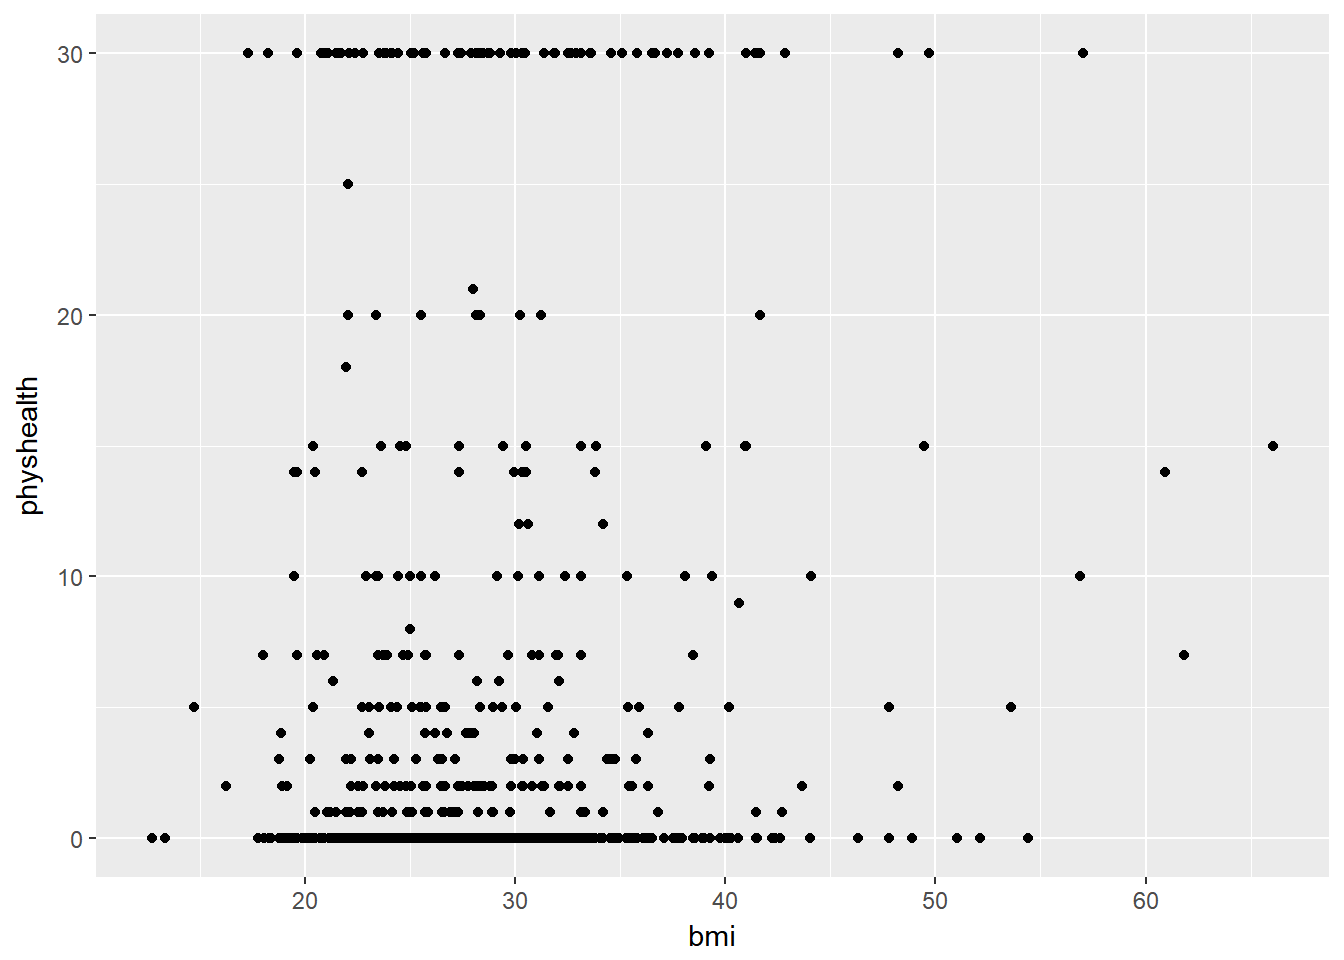
\includegraphics{bookdown-demo_files/figure-latex/scatter_physhealth_bmi_1-1.pdf}

A good question to ask ourselves here might be: ``In what BMI range can
we make a reasonable prediction of \texttt{physhealth}?''

Now, we might take the plot above and add a simple linear model \ldots{}

\begin{Shaded}
\begin{Highlighting}[]
\KeywordTok{ggplot}\NormalTok{(}\DataTypeTok{data =}\NormalTok{ smartcle2, }\KeywordTok{aes}\NormalTok{(}\DataTypeTok{x =}\NormalTok{ bmi, }\DataTypeTok{y =}\NormalTok{ physhealth)) }\OperatorTok{+}
\StringTok{    }\KeywordTok{geom_point}\NormalTok{() }\OperatorTok{+}
\StringTok{    }\KeywordTok{geom_smooth}\NormalTok{(}\DataTypeTok{method =} \StringTok{"lm"}\NormalTok{, }\DataTypeTok{se =} \OtherTok{FALSE}\NormalTok{)}
\end{Highlighting}
\end{Shaded}

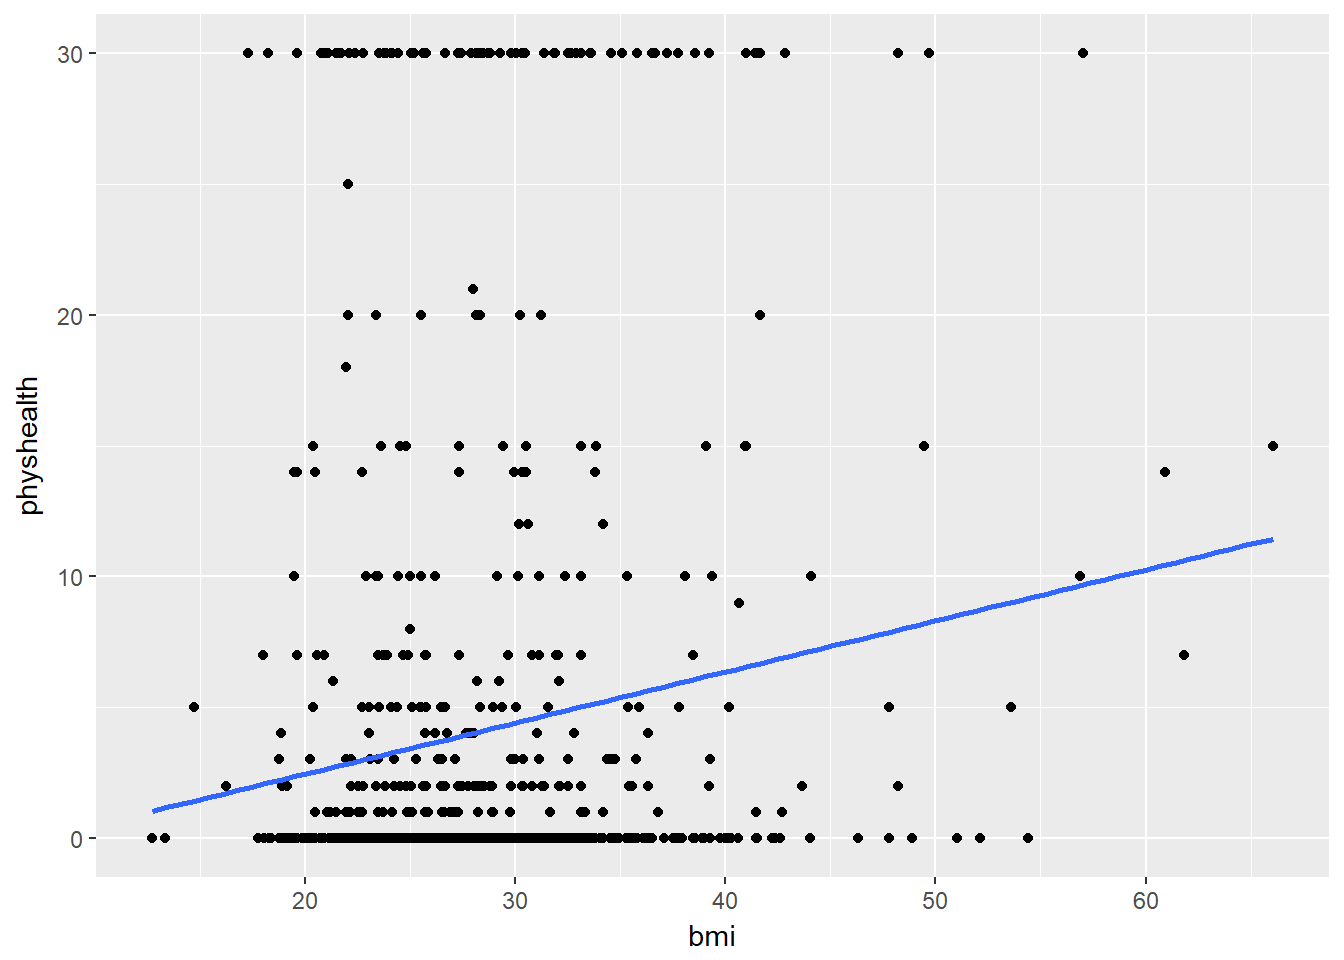
\includegraphics{bookdown-demo_files/figure-latex/c2_scatter_physhealth_bmi_2-1.pdf}

which shows the same least squares regression model that we can fit with
the \texttt{lm} command.

\subsection{Fitting a Simple Regression
Model}\label{fitting-a-simple-regression-model}

\begin{Shaded}
\begin{Highlighting}[]
\NormalTok{model_A <-}\StringTok{ }\KeywordTok{lm}\NormalTok{(physhealth }\OperatorTok{~}\StringTok{ }\NormalTok{bmi, }\DataTypeTok{data =}\NormalTok{ smartcle2)}

\NormalTok{model_A}
\end{Highlighting}
\end{Shaded}

\begin{verbatim}

Call:
lm(formula = physhealth ~ bmi, data = smartcle2)

Coefficients:
(Intercept)          bmi  
    -1.4514       0.1953  
\end{verbatim}

\begin{Shaded}
\begin{Highlighting}[]
\KeywordTok{summary}\NormalTok{(model_A)}
\end{Highlighting}
\end{Shaded}

\begin{verbatim}

Call:
lm(formula = physhealth ~ bmi, data = smartcle2)

Residuals:
   Min     1Q Median     3Q    Max 
-9.171 -4.057 -3.193 -1.576 28.073 

Coefficients:
            Estimate Std. Error t value Pr(>|t|)    
(Intercept) -1.45143    1.29185  -1.124    0.262    
bmi          0.19527    0.04521   4.319 1.74e-05 ***
---
Signif. codes:  0 '***' 0.001 '**' 0.01 '*' 0.05 '.' 0.1 ' ' 1

Residual standard error: 8.556 on 894 degrees of freedom
Multiple R-squared:  0.02044,   Adjusted R-squared:  0.01934 
F-statistic: 18.65 on 1 and 894 DF,  p-value: 1.742e-05
\end{verbatim}

\begin{Shaded}
\begin{Highlighting}[]
\KeywordTok{confint}\NormalTok{(model_A, }\DataTypeTok{level =} \FloatTok{0.95}\NormalTok{)}
\end{Highlighting}
\end{Shaded}

\begin{verbatim}
                 2.5 %    97.5 %
(Intercept) -3.9868457 1.0839862
bmi          0.1065409 0.2840068
\end{verbatim}

The model coefficients can be obtained by printing the model object, and
the \texttt{summary} function provides several useful descriptions of
the model's residuals, its statistical significance, and quality of fit.

\subsection{Model Summary for a Simple (One-Predictor)
Regression}\label{model-summary-for-a-simple-one-predictor-regression}

The fitted model predicts \texttt{physhealth} with the equation -1.45 +
0.195*\texttt{bmi}, as we can read off from the model coefficients.

Each of the 896 respondents included in the \texttt{smartcle2} data
makes a contribution to this model.

\subsubsection{Residuals}\label{residuals}

Suppose Harry is one of the people in that group, and Harry's data is
\texttt{bmi} = 20, and \texttt{physhealth} = 3.

\begin{itemize}
\tightlist
\item
  Harry's \emph{observed} value of \texttt{physhealth} is just the value
  we have in the data for them, in this case, observed
  \texttt{physhealth} = 3 for Harry.
\item
  Harry's \emph{fitted} or \emph{predicted} \texttt{physhealth} value is
  the result of calculating -1.45 + 0.195*\texttt{bmi} for Harry. So, if
  Harry's BMI was 20, then Harry's predicted \texttt{physhealth} value
  is -1.45 + (0.195)(20) = 2.45.
\item
  The \emph{residual} for Harry is then his \emph{observed} outcome
  minus his \emph{fitted} outcome, so Harry has a residual of 3 - 2.45 =
  0.55.
\item
  Graphically, a residual represents vertical distance between the
  observed point and the fitted regression line.
\item
  Points above the regression line will have positive residuals, and
  points below the regression line will have negative residuals. Points
  on the line have zero residuals.
\end{itemize}

The residuals are summarized at the top of the \texttt{summary} output
for linear model.

\begin{itemize}
\tightlist
\item
  The mean residual will always be zero in an ordinary least squares
  model, but a five number summary of the residuals is provided by the
  summary, as is an estimated standard deviation of the residuals
  (called here the Residual standard error.)
\item
  In the \texttt{smartcle2} data, the minimum residual was -9.17, so for
  one subject, the observed value was 9.17 days smaller than the
  predicted value. This means that the prediction was 9.17 days too
  large for that subject.
\item
  Similarly, the maximum residual was 28.07 days, so for one subject the
  prediction was 28.07 days too small. Not a strong performance.
\item
  In a least squares model, the residuals are assumed to follow a Normal
  distribution, with mean zero, and standard deviation (for the
  \texttt{smartcle2} data) of about 8.6 days. Thus, by the definition of
  a Normal distribution, we'd expect
\item
  about 68\% of the residuals to be between -8.6 and +8.6 days,
\item
  about 95\% of the residuals to be between -17.2 and +17.2 days,
\item
  about all (99.7\%) of the residuals to be between -25.8 and +25.8
  days.
\end{itemize}

\subsubsection{Coefficients section}\label{coefficients-section}

The \texttt{summary} for a linear model shows Estimates, Standard
Errors, t values and \emph{p} values for each coefficient fit.

\begin{itemize}
\tightlist
\item
  The Estimates are the point estimates of the intercept and slope of
  \texttt{bmi} in our model.
\item
  In this case, our estimated slope is 0.195, which implies that if
  Harry's BMI is 20 and Sally's BMI is 21, we predict that Sally's
  \texttt{physhealth} will be 0.195 days larger than Harry's.
\item
  The Standard Errors are also provided for each estimate. We can create
  rough 95\% confidence intervals by adding and subtracting two standard
  errors from each coefficient, or we can get a slightly more accurate
  answer with the \texttt{confint} function.
\item
  Here, the 95\% confidence interval for the slope of \texttt{bmi} is
  estimated to be (0.11, 0.28). This is a good measure of the
  uncertainty in the slope that is captured by our model. We are 95\%
  confident in the process of building this interval, but this doesn't
  mean we're 95\% sure that the true slope is actually in that interval.
\end{itemize}

Also available are a \emph{t} value (just the Estimate divided by the
Standard Error) and the appropriate \emph{p} value for testing the null
hypothesis that the true value of the coefficient is 0 against a
two-tailed alternative.

\begin{itemize}
\tightlist
\item
  If a slope coefficient is statistically significantly different from
  0, this implies that 0 will not be part of the uncertainty interval
  obtained through \texttt{confint}.
\item
  If the slope was zero, it would suggest that \texttt{bmi} would add no
  predictive value to the model. But that's unlikely here.
\end{itemize}

If the \texttt{bmi} slope coefficient is associated with a small
\emph{p} value, as in the case of our \texttt{model\_A}, it suggests
that the model including \texttt{bmi} is statistically significantly
better at predicting \texttt{physhealth} than the model without
\texttt{bmi}.

\begin{itemize}
\tightlist
\item
  Without \texttt{bmi} our \texttt{model\_A} would become an
  \emph{intercept-only} model, in this case, which would predict the
  mean \texttt{physhealth} for everyone, regardless of any other
  information.
\end{itemize}

\subsubsection{Model Fit Summaries}\label{model-fit-summaries}

The \texttt{summary} of a linear model also displays:

\begin{itemize}
\tightlist
\item
  The residual standard error and associated degrees of freedom for the
  residuals.
\item
  For a simple (one-predictor) least regression like this, the residual
  degrees of freedom will be the sample size minus 2.
\item
  The multiple R-squared (or coefficient of determination)
\item
  This is interpreted as the proportion of variation in the outcome
  (\texttt{physhealth}) accounted for by the model, and will always fall
  between 0 and 1 as a result.
\item
  Our model\_A accounts for a mere 2\% of the variation in
  \texttt{physhealth}.
\item
  The Adjusted R-squared value ``adjusts'' for the size of our model in
  terms of the number of coefficients included in the model.
\item
  The adjusted R-squared will always be less than the Multiple
  R-squared.
\item
  We still hope to find models with relatively large adjusted
  R\textsuperscript{2} values.
\item
  In particular, we hope to find models where the adjusted
  R\textsuperscript{2} isn't substantially less than the Multiple
  R-squared.
\item
  The adjusted R-squared is usually a better estimate of likely
  performance of our model in new data than is the Multiple R-squared.
\item
  The adjusted R-squared result is no longer interpretable as a
  proportion of anything - in fact, it can fall below 0.
\item
  We can obtain the adjusted R\textsuperscript{2} from the raw
  R\textsuperscript{2}, the number of observations \emph{N} and the
  number of predictors \emph{p} included in the model, as follows:
\end{itemize}

\[
R^2_{adj} = 1 - \frac{(1 - R^2)(N - 1)}{N - p - 1},
\]

\begin{itemize}
\tightlist
\item
  The F statistic and \emph{p} value from a global ANOVA test of the
  model.

  \begin{itemize}
  \tightlist
  \item
    Obtaining a statistically significant result here is usually pretty
    straightforward, since the comparison is between our model, and a
    model which simply predicts the mean value of the outcome for
    everyone.
  \item
    In a simple (one-predictor) linear regression like this, the t
    statistic for the slope is just the square root of the F statistic,
    and the resulting \emph{p} values for the slope's t test and for the
    global F test will be identical.
  \end{itemize}
\item
  To see the complete ANOVA F test for this model, we can run
  \texttt{anova(model\_A)}.
\end{itemize}

\begin{Shaded}
\begin{Highlighting}[]
\KeywordTok{anova}\NormalTok{(model_A)}
\end{Highlighting}
\end{Shaded}

\begin{verbatim}
Analysis of Variance Table

Response: physhealth
           Df Sum Sq Mean Sq F value    Pr(>F)    
bmi         1   1366  1365.5  18.655 1.742e-05 ***
Residuals 894  65441    73.2                      
---
Signif. codes:  0 '***' 0.001 '**' 0.01 '*' 0.05 '.' 0.1 ' ' 1
\end{verbatim}

\subsection{\texorpdfstring{Using the \texttt{broom}
package}{Using the broom package}}\label{using-the-broom-package}

The \texttt{broom} package has three functions of particular use in a
linear regression model:

\subsubsection{\texorpdfstring{The \texttt{tidy}
function}{The tidy function}}\label{the-tidy-function}

\texttt{tidy} builds a data frame/tibble containing information about
the coefficients in the model, their standard errors, t statistics and
\emph{p} values.

\begin{Shaded}
\begin{Highlighting}[]
\KeywordTok{tidy}\NormalTok{(model_A)}
\end{Highlighting}
\end{Shaded}

\begin{verbatim}
         term   estimate  std.error statistic      p.value
1 (Intercept) -1.4514298 1.29185199 -1.123526 2.615156e-01
2         bmi  0.1952739 0.04521145  4.319125 1.741859e-05
\end{verbatim}

\subsubsection{\texorpdfstring{The \texttt{glance}
function}{The glance function}}\label{the-glance-function}

glance` builds a data frame/tibble containing summary statistics about
the model, including

\begin{itemize}
\tightlist
\item
  the (raw) multiple R\textsuperscript{2} and adjusted R\^{}2
\item
  \texttt{sigma} which is the residual standard error
\item
  the F \texttt{statistic}, \texttt{p.value} model \texttt{df} and
  \texttt{df.residual} associated with the global ANOVA test, plus
\item
  several statistics that will be useful in comparing models down the
  line:
\item
  the model's log likelihood function value, \texttt{logLik}
\item
  the model's Akaike's Information Criterion value, \texttt{AIC}
\item
  the model's Bayesian Information Criterion value, \texttt{BIC}
\item
  and the model's \texttt{deviance} statistic
\end{itemize}

\begin{Shaded}
\begin{Highlighting}[]
\KeywordTok{glance}\NormalTok{(model_A)}
\end{Highlighting}
\end{Shaded}

\begin{verbatim}
   r.squared adj.r.squared    sigma statistic      p.value df    logLik
1 0.02044019    0.01934449 8.555737  18.65484 1.741859e-05  2 -3193.723
       AIC     BIC deviance df.residual
1 6393.446 6407.84 65441.36         894
\end{verbatim}

\subsubsection{\texorpdfstring{The \texttt{augment}
function}{The augment function}}\label{the-augment-function}

\texttt{augment} builds a data frame/tibble which adds fitted values,
residuals and other diagnostic summaries that describe each observation
to the original data used to fit the model, and this includes

\begin{itemize}
\tightlist
\item
  \texttt{.fitted} and \texttt{.resid}, the fitted and residual values,
  in addition to
\item
  \texttt{.hat}, the leverage value for this observation
\item
  \texttt{.cooksd}, the Cook's distance measure of \emph{influence} for
  this observation
\item
  \texttt{.stdresid}, the standardized residual (think of this as a
  z-score - a measure of the residual divided by its associated standard
  deviation \texttt{.sigma})
\item
  and \texttt{se.fit} which will help us generate prediction intervals
  for the model downstream
\end{itemize}

Note that each of the new columns begins with \texttt{.} to avoid
overwriting any data.

\begin{Shaded}
\begin{Highlighting}[]
\KeywordTok{head}\NormalTok{(}\KeywordTok{augment}\NormalTok{(model_A))}
\end{Highlighting}
\end{Shaded}

\begin{verbatim}
  physhealth   bmi  .fitted   .se.fit      .resid        .hat   .sigma
1          0 26.69 3.760430 0.2907252 -3.76043009 0.001154651 8.559600
2          0 23.70 3.176561 0.3422908 -3.17656119 0.001600574 8.559865
3          1 26.92 3.805343 0.2890054 -2.80534308 0.001141030 8.560010
4          0 21.66 2.778202 0.4005101 -2.77820248 0.002191352 8.560020
5          5 24.09 3.252718 0.3329154  1.74728200 0.001514095 8.560326
6          4 27.64 3.945940 0.2860087  0.05405972 0.001117490 8.560526
       .cooksd   .std.resid
1 1.117852e-04 -0.439775451
2 1.106717e-04 -0.371575999
3 6.147744e-05 -0.328077528
4 1.160381e-04 -0.325074461
5 3.167016e-05  0.204378225
6 2.235722e-08  0.006322069
\end{verbatim}

For more on the \texttt{broom} package, you may want to look at
\href{https://cran.r-project.org/web/packages/broom/vignettes/broom.html}{this
vignette}.

\subsection{How does the model do? (Residuals vs.~Fitted
Values)}\label{how-does-the-model-do-residuals-vs.fitted-values}

\begin{itemize}
\tightlist
\item
  Remember that the R\textsuperscript{2} value was about 2\%.
\end{itemize}

\begin{Shaded}
\begin{Highlighting}[]
\KeywordTok{plot}\NormalTok{(model_A, }\DataTypeTok{which =} \DecValTok{1}\NormalTok{)}
\end{Highlighting}
\end{Shaded}

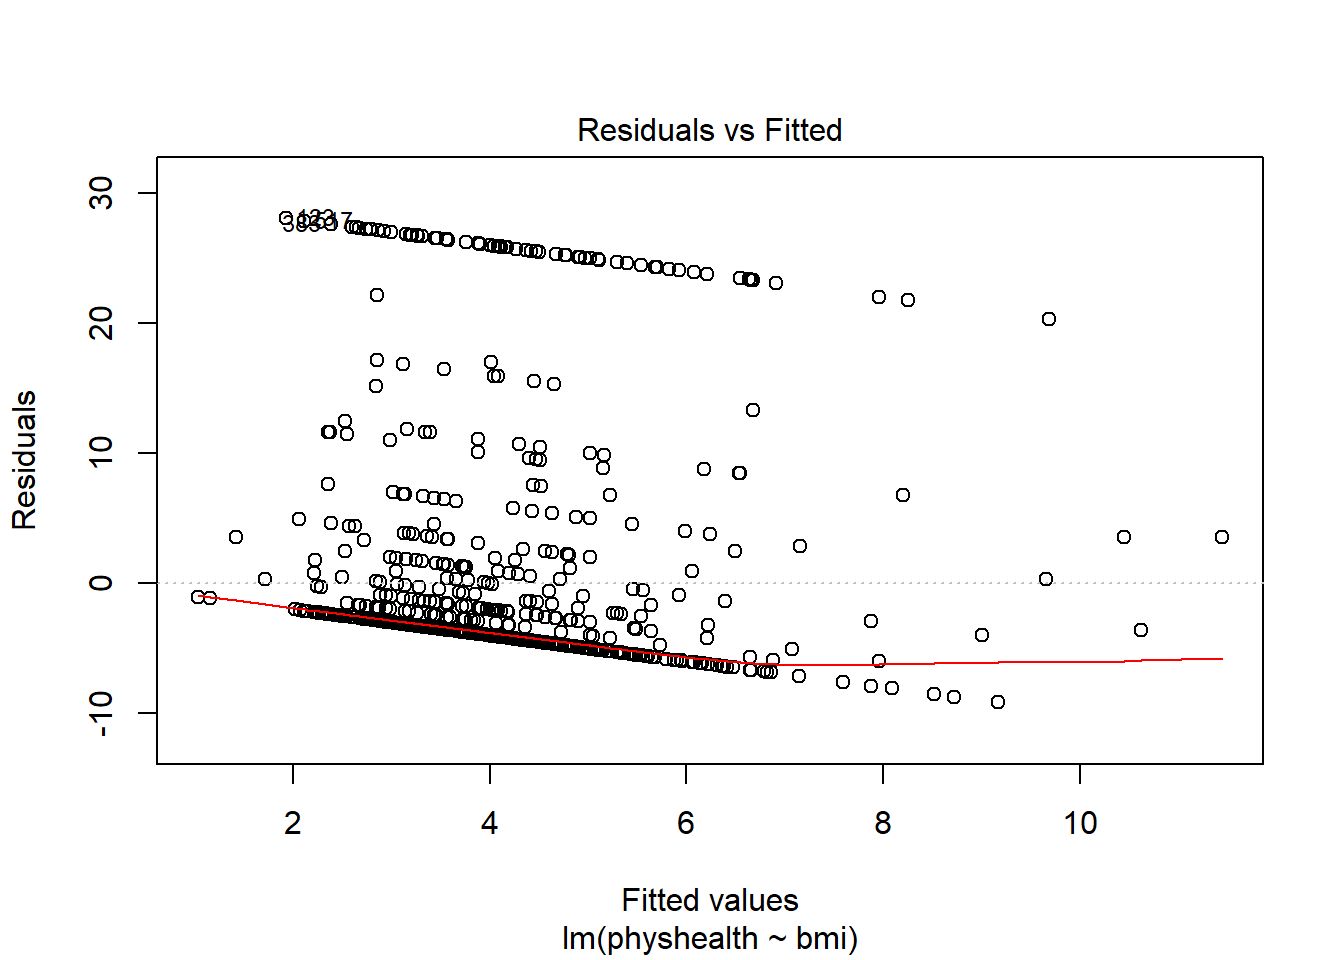
\includegraphics{bookdown-demo_files/figure-latex/chapter2_first_resid_plot_model_A-1.pdf}

This is a plot of residuals vs.~fitted values. The goal here is for this
plot to look like a random scatter of points, perhaps like a ``fuzzy
football'', and that's \textbf{not} what we have. Why?

If you prefer, here's a \texttt{ggplot2} version of a similar plot, now
looking at standardized residuals instead of raw residuals, and adding a
loess smooth and a linear fit to the result.

\begin{Shaded}
\begin{Highlighting}[]
\KeywordTok{ggplot}\NormalTok{(}\KeywordTok{augment}\NormalTok{(model_A), }\KeywordTok{aes}\NormalTok{(}\DataTypeTok{x =}\NormalTok{ .fitted, }\DataTypeTok{y =}\NormalTok{ .std.resid)) }\OperatorTok{+}
\StringTok{    }\KeywordTok{geom_point}\NormalTok{() }\OperatorTok{+}
\StringTok{    }\KeywordTok{geom_smooth}\NormalTok{(}\DataTypeTok{method =} \StringTok{"lm"}\NormalTok{, }\DataTypeTok{se =} \OtherTok{FALSE}\NormalTok{, }\DataTypeTok{col =} \StringTok{"red"}\NormalTok{, }\DataTypeTok{linetype =} \StringTok{"dashed"}\NormalTok{) }\OperatorTok{+}
\StringTok{    }\KeywordTok{geom_smooth}\NormalTok{(}\DataTypeTok{method =} \StringTok{"loess"}\NormalTok{, }\DataTypeTok{se =} \OtherTok{FALSE}\NormalTok{, }\DataTypeTok{col =} \StringTok{"navy"}\NormalTok{) }\OperatorTok{+}
\StringTok{    }\KeywordTok{theme_bw}\NormalTok{()}
\end{Highlighting}
\end{Shaded}

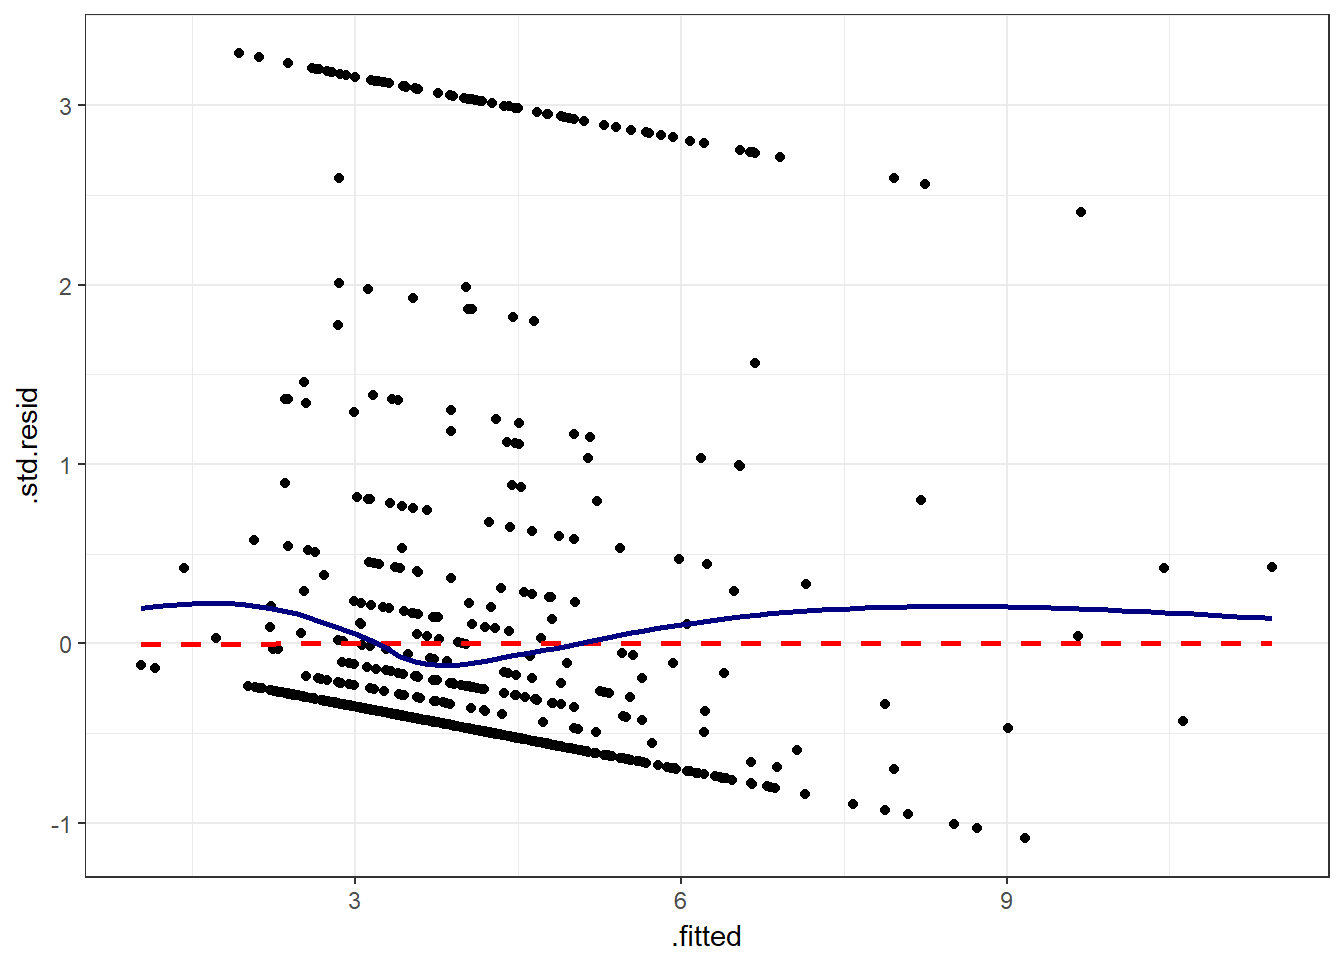
\includegraphics{bookdown-demo_files/figure-latex/chapter2_ggplot_first_resid_plot_model_A-1.pdf}

The problem we're having here becomes, I think, a little more obvious if
we look at what we're predicting. Does \texttt{physhealth} look like a
good candidate for a linear model?

\begin{Shaded}
\begin{Highlighting}[]
\KeywordTok{ggplot}\NormalTok{(smartcle2, }\KeywordTok{aes}\NormalTok{(}\DataTypeTok{x =}\NormalTok{ physhealth)) }\OperatorTok{+}
\KeywordTok{geom_histogram}\NormalTok{(}\DataTypeTok{bins =} \DecValTok{30}\NormalTok{, }\DataTypeTok{fill =} \StringTok{"dodgerblue"}\NormalTok{, }\DataTypeTok{color =} \StringTok{"royalblue"}\NormalTok{)}
\end{Highlighting}
\end{Shaded}

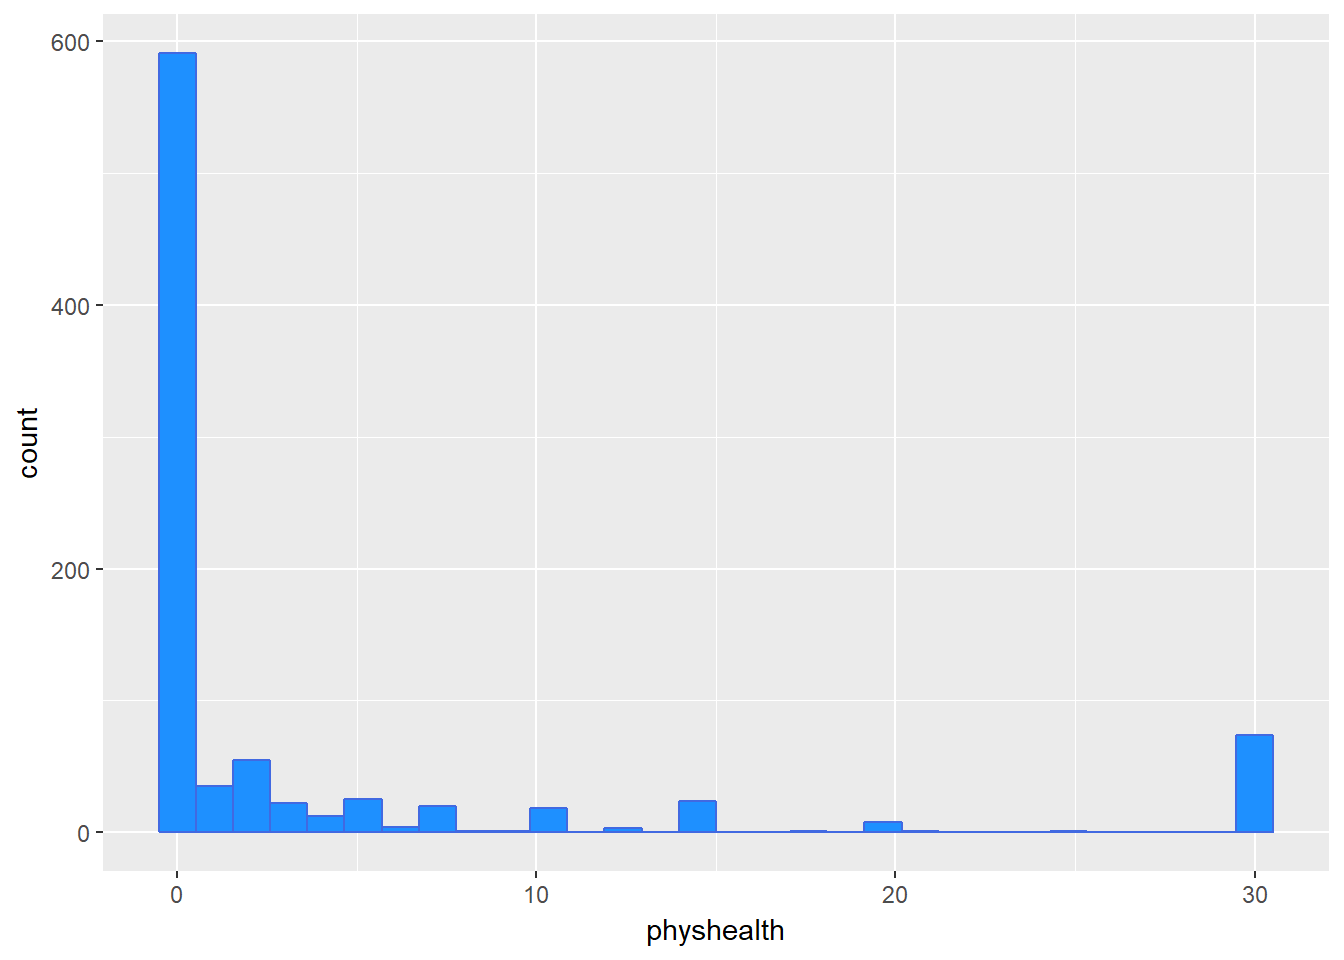
\includegraphics{bookdown-demo_files/figure-latex/histogram_of_physhealth_smartcle2-1.pdf}

\begin{Shaded}
\begin{Highlighting}[]
\NormalTok{smartcle2 }\OperatorTok\StringTok{ }\KeywordTok{count}\NormalTok{(physhealth }\OperatorTok{==}\StringTok{ }\DecValTok{0}\NormalTok{, physhealth }\OperatorTok{==}\StringTok{ }\DecValTok{30}\NormalTok{)}
\end{Highlighting}
\end{Shaded}

\begin{verbatim}
# A tibble: 3 x 3
  `physhealth == 0` `physhealth == 30`     n
  <lgl>             <lgl>              <int>
1 F                 F                    231
2 F                 T                     74
3 T                 F                    591
\end{verbatim}

No matter what model we fit, if we are predicting \texttt{physhealth},
and most of the data are values of 0 and 30, we have limited variation
in our outcome, and so our linear model will be somewhat questionable
just on that basis.

A normal Q-Q plot of the standardized residuals for our
\texttt{model\_A} shows this problem, too.

\begin{Shaded}
\begin{Highlighting}[]
\KeywordTok{plot}\NormalTok{(model_A, }\DataTypeTok{which =} \DecValTok{2}\NormalTok{)}
\end{Highlighting}
\end{Shaded}

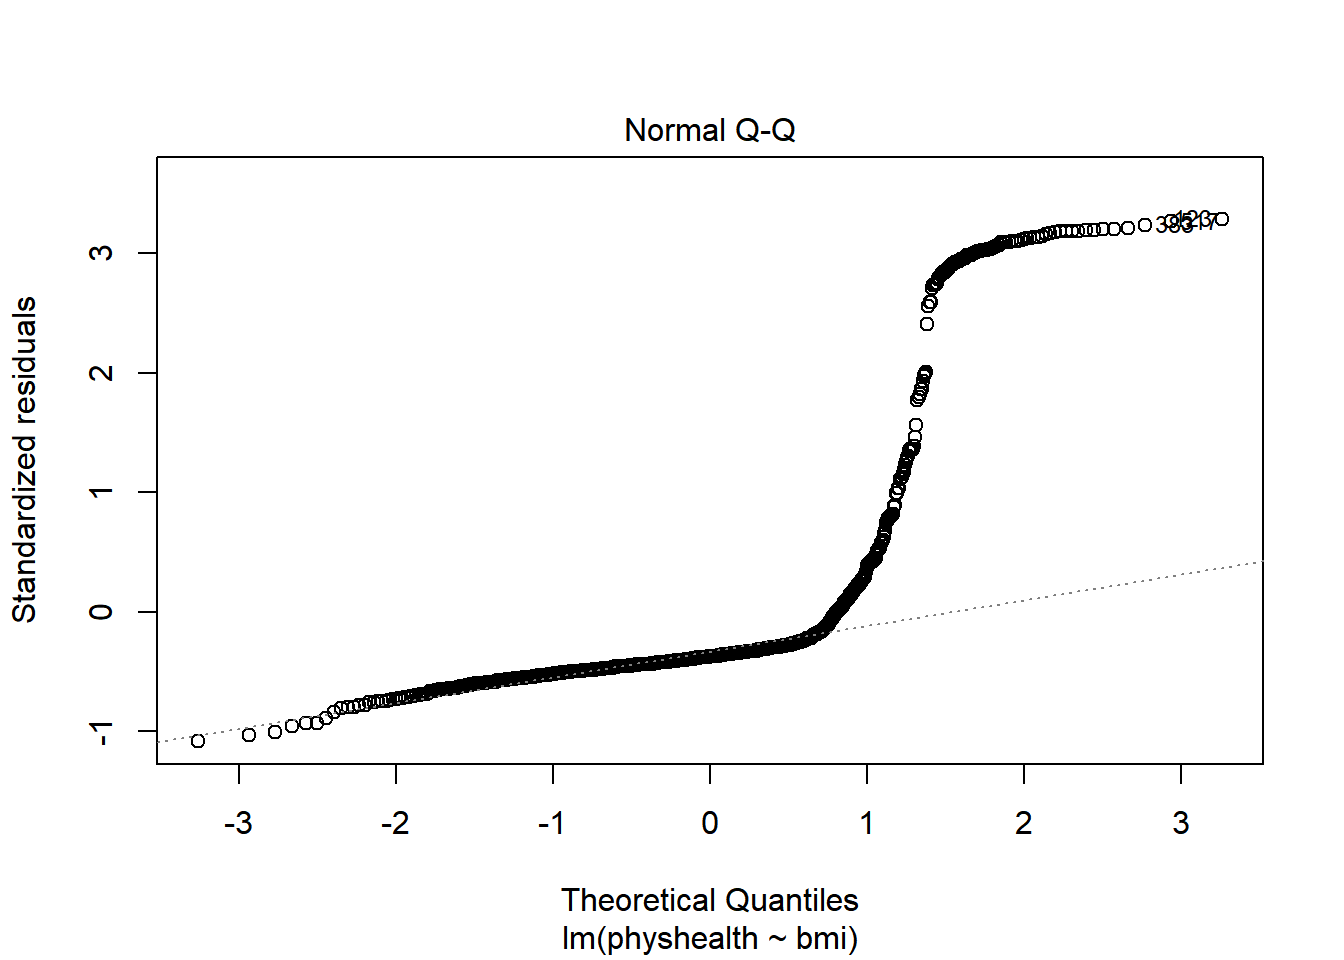
\includegraphics{bookdown-demo_files/figure-latex/chapter2_second_resid_plot_model_A-1.pdf}

We're going to need a method to deal with this sort of outcome, that has
both a floor and a ceiling. We'll get there eventually, but linear
regression alone doesn't look promising.

All right, so that didn't go anywhere great. Let's try again, with a new
outcome.

\section{A New Small Study: Predicting
BMI}\label{a-new-small-study-predicting-bmi}

We'll begin by investigating the problem of predicting \texttt{bmi}, at
first with just three regression inputs: \texttt{sex}, \texttt{exerany}
and \texttt{sleephrs}, in our new \texttt{smartcle2} data set.

\begin{itemize}
\tightlist
\item
  The outcome of interest is \texttt{bmi}.
\item
  Inputs to the regression model are:

  \begin{itemize}
  \tightlist
  \item
    \texttt{female} = 1 if the subject is female, and 0 if they are male
  \item
    \texttt{exerany} = 1 if the subject exercised in the past 30 days,
    and 0 if they didn't
  \item
    \texttt{sleephrs} = hours slept in a typical 24-hour period (treated
    as quantitative)
  \end{itemize}
\end{itemize}

\subsection{\texorpdfstring{Does \texttt{female} predict \texttt{bmi}
well?}{Does female predict bmi well?}}\label{does-female-predict-bmi-well}

\subsubsection{Graphical Assessment}\label{graphical-assessment}

\begin{Shaded}
\begin{Highlighting}[]
\KeywordTok{ggplot}\NormalTok{(smartcle2, }\KeywordTok{aes}\NormalTok{(}\DataTypeTok{x =}\NormalTok{ female, }\DataTypeTok{y =}\NormalTok{ bmi)) }\OperatorTok{+}
\StringTok{    }\KeywordTok{geom_point}\NormalTok{()}
\end{Highlighting}
\end{Shaded}

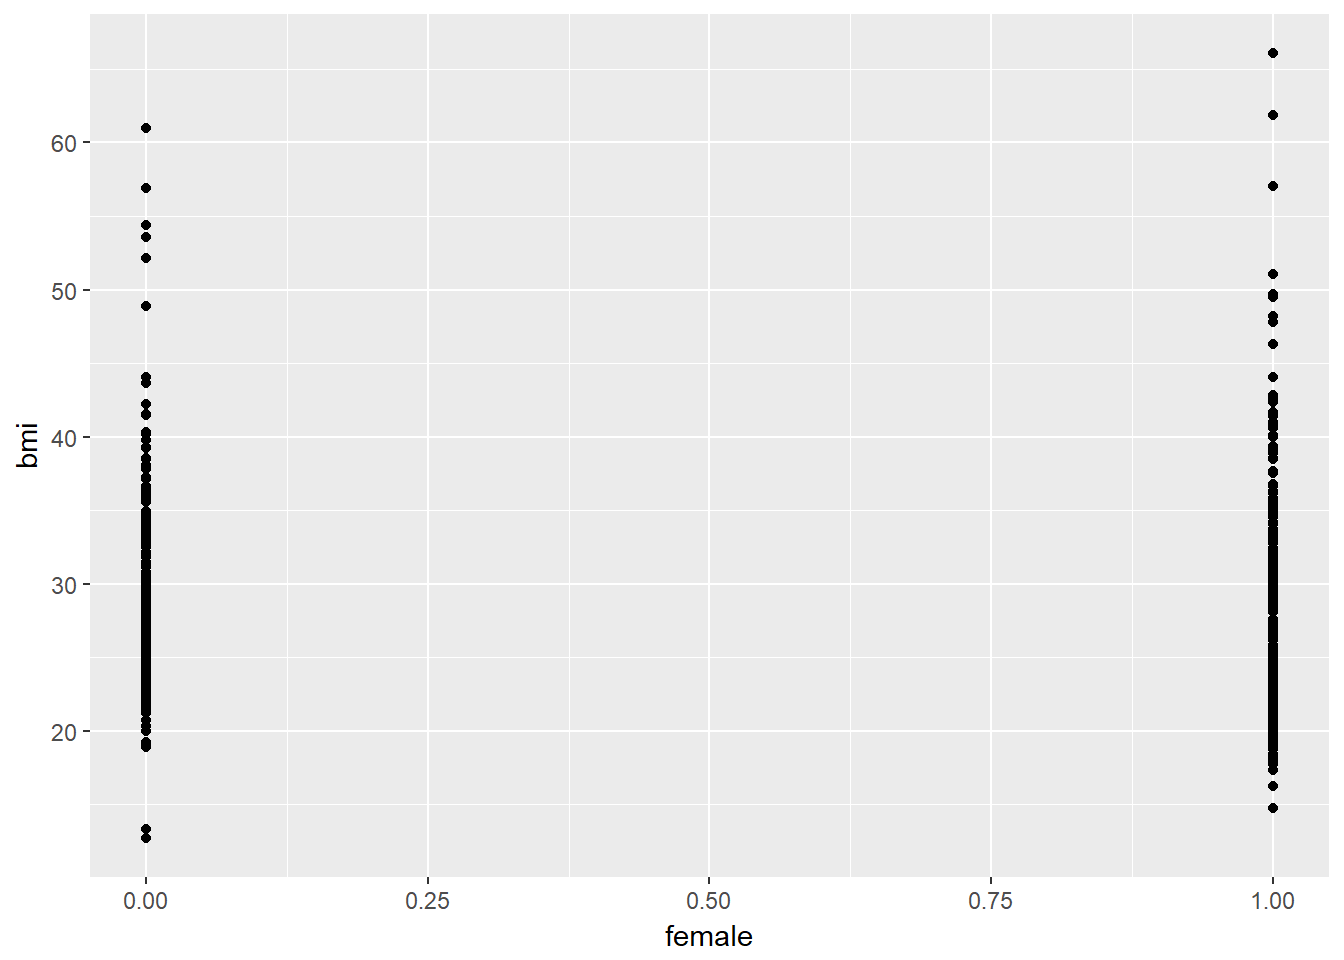
\includegraphics{bookdown-demo_files/figure-latex/c2_sex_bmi_plot1-1.pdf}

Not so helpful. We should probably specify that \texttt{female} is a
factor, and try another plotting approach.

\begin{Shaded}
\begin{Highlighting}[]
\KeywordTok{ggplot}\NormalTok{(smartcle2, }\KeywordTok{aes}\NormalTok{(}\DataTypeTok{x =} \KeywordTok{factor}\NormalTok{(female), }\DataTypeTok{y =}\NormalTok{ bmi)) }\OperatorTok{+}
\StringTok{    }\KeywordTok{geom_boxplot}\NormalTok{()}
\end{Highlighting}
\end{Shaded}

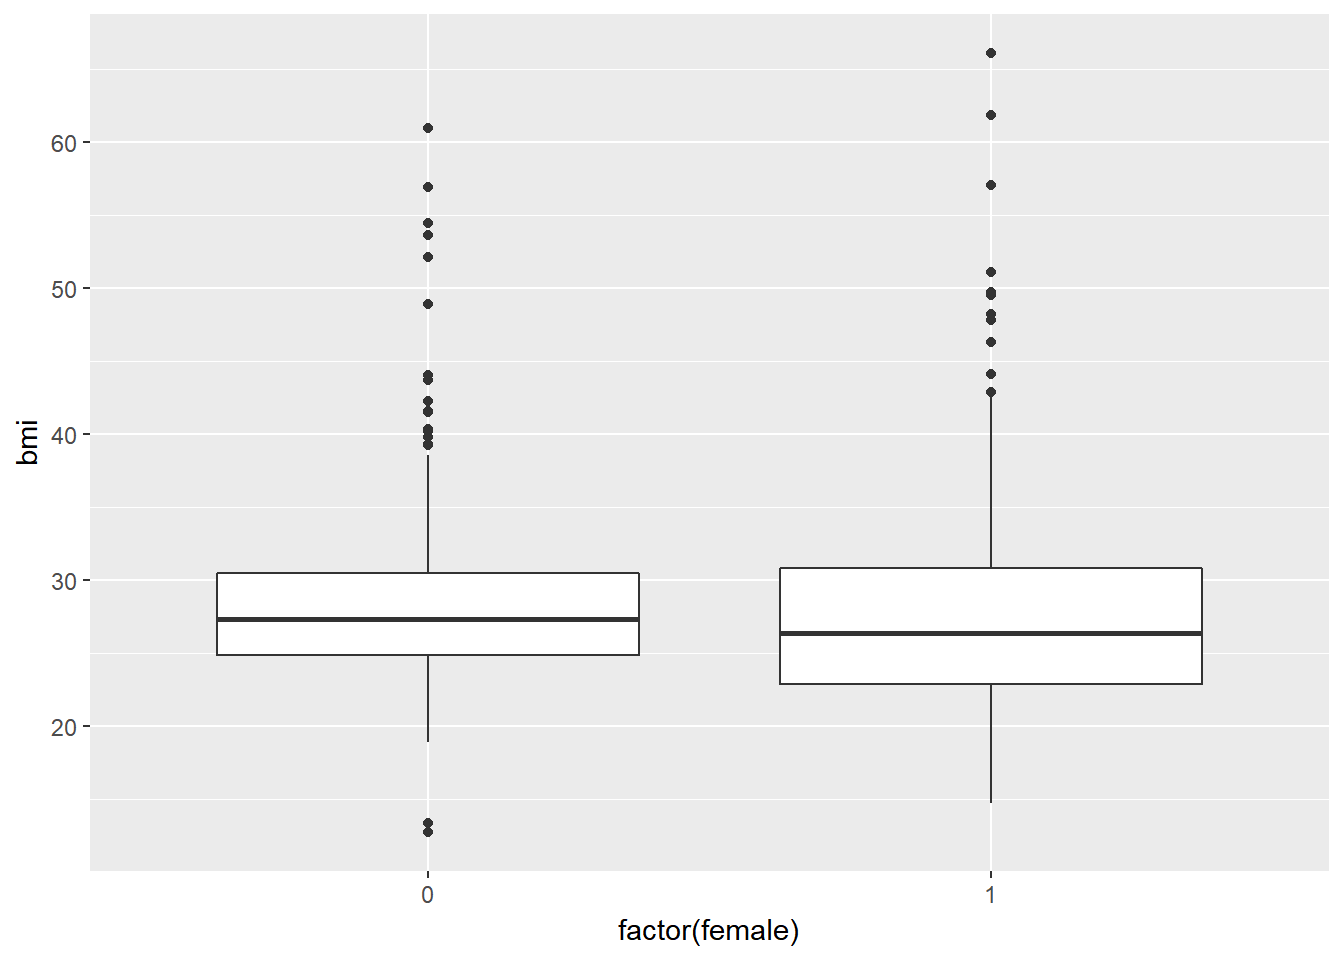
\includegraphics{bookdown-demo_files/figure-latex/c2_sex_bmi_plot2-1.pdf}

The median BMI looks a little higher for males. Let's see if a model
reflects that.

\section{\texorpdfstring{\texttt{c2\_m1}: A simple t-test
model}{c2\_m1: A simple t-test model}}\label{c2_m1-a-simple-t-test-model}

\begin{Shaded}
\begin{Highlighting}[]
\NormalTok{c2_m1 <-}\StringTok{ }\KeywordTok{lm}\NormalTok{(bmi }\OperatorTok{~}\StringTok{ }\NormalTok{female, }\DataTypeTok{data =}\NormalTok{ smartcle2)}
\NormalTok{c2_m1}
\end{Highlighting}
\end{Shaded}

\begin{verbatim}

Call:
lm(formula = bmi ~ female, data = smartcle2)

Coefficients:
(Intercept)       female  
    28.3600      -0.8457  
\end{verbatim}

\begin{Shaded}
\begin{Highlighting}[]
\KeywordTok{summary}\NormalTok{(c2_m1)}
\end{Highlighting}
\end{Shaded}

\begin{verbatim}

Call:
lm(formula = bmi ~ female, data = smartcle2)

Residuals:
    Min      1Q  Median      3Q     Max 
-15.650  -4.129  -1.080   2.727  38.546 

Coefficients:
            Estimate Std. Error t value Pr(>|t|)    
(Intercept)  28.3600     0.3274  86.613   <2e-16 ***
female       -0.8457     0.4282  -1.975   0.0485 *  
---
Signif. codes:  0 '***' 0.001 '**' 0.01 '*' 0.05 '.' 0.1 ' ' 1

Residual standard error: 6.315 on 894 degrees of freedom
Multiple R-squared:  0.004345,  Adjusted R-squared:  0.003231 
F-statistic: 3.902 on 1 and 894 DF,  p-value: 0.04855
\end{verbatim}

\begin{Shaded}
\begin{Highlighting}[]
\KeywordTok{confint}\NormalTok{(c2_m1)}
\end{Highlighting}
\end{Shaded}

\begin{verbatim}
                2.5 %      97.5 %
(Intercept) 27.717372 29.00262801
female      -1.686052 -0.00539878
\end{verbatim}

The model suggests, based on these 896 subjects, that

\begin{itemize}
\tightlist
\item
  our best prediction for males is BMI = 28.36 kg/m\textsuperscript{2},
  and
\item
  our best prediction for females is BMI = 28.36 - 0.85 = 27.51
  kg/m\textsuperscript{2}.
\item
  the mean difference between females and males is -0.85
  kg/m\textsuperscript{2} in BMI
\item
  a 95\% confidence (uncertainty) interval for that mean female - male
  difference in BMI ranges from -1.69 to -0.01
\item
  the model accounts for 0.4\% of the variation in BMI, so that knowing
  the respondent's sex does very little to reduce the size of the
  prediction errors as compared to an intercept only model that would
  predict the overall mean (regardless of sex) for all subjects.
\item
  the model makes some enormous errors, with one subject being predicted
  to have a BMI 38 points lower than his/her actual BMI.
\end{itemize}

Note that this simple regression model just gives us the t-test.

\begin{Shaded}
\begin{Highlighting}[]
\KeywordTok{t.test}\NormalTok{(bmi }\OperatorTok{~}\StringTok{ }\NormalTok{female, }\DataTypeTok{var.equal =} \OtherTok{TRUE}\NormalTok{, }\DataTypeTok{data =}\NormalTok{ smartcle2)}
\end{Highlighting}
\end{Shaded}

\begin{verbatim}

    Two Sample t-test

data:  bmi by female
t = 1.9752, df = 894, p-value = 0.04855
alternative hypothesis: true difference in means is not equal to 0
95 percent confidence interval:
 0.00539878 1.68605160
sample estimates:
mean in group 0 mean in group 1 
       28.36000        27.51427 
\end{verbatim}

\section{\texorpdfstring{\texttt{c2\_m2}: Adding another predictor
(two-way ANOVA without
interaction)}{c2\_m2: Adding another predictor (two-way ANOVA without interaction)}}\label{c2_m2-adding-another-predictor-two-way-anova-without-interaction}

When we add in the information about \texttt{exerany} to our original
model, we might first picture the data. We could look at separate
histograms,

\begin{Shaded}
\begin{Highlighting}[]
\KeywordTok{ggplot}\NormalTok{(smartcle2, }\KeywordTok{aes}\NormalTok{(}\DataTypeTok{x =}\NormalTok{ bmi)) }\OperatorTok{+}
\StringTok{    }\KeywordTok{geom_histogram}\NormalTok{(}\DataTypeTok{bins =} \DecValTok{30}\NormalTok{) }\OperatorTok{+}
\StringTok{    }\KeywordTok{facet_grid}\NormalTok{(female }\OperatorTok{~}\StringTok{ }\NormalTok{exerany, }\DataTypeTok{labeller =}\NormalTok{ label_both)}
\end{Highlighting}
\end{Shaded}

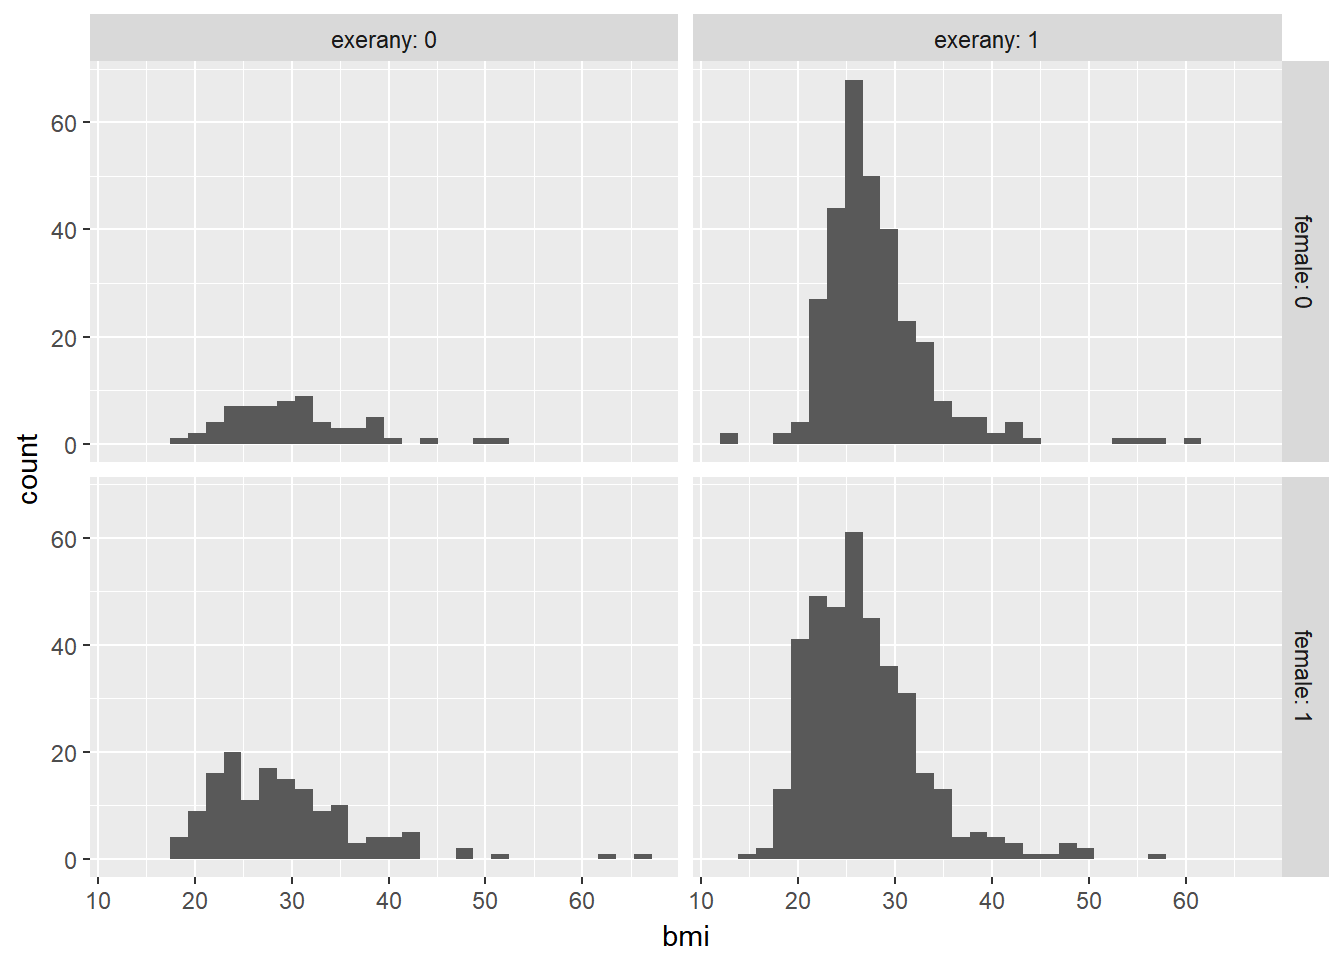
\includegraphics{bookdown-demo_files/figure-latex/c2_smartcle2_plot_bmi_hist_by_female_exerany-1.pdf}

or maybe boxplots?

\begin{Shaded}
\begin{Highlighting}[]
\KeywordTok{ggplot}\NormalTok{(smartcle2, }\KeywordTok{aes}\NormalTok{(}\DataTypeTok{x =} \KeywordTok{factor}\NormalTok{(female), }\DataTypeTok{y =}\NormalTok{ bmi)) }\OperatorTok{+}
\StringTok{    }\KeywordTok{geom_boxplot}\NormalTok{() }\OperatorTok{+}
\StringTok{    }\KeywordTok{facet_wrap}\NormalTok{(}\OperatorTok{~}\StringTok{ }\NormalTok{exerany, }\DataTypeTok{labeller =}\NormalTok{ label_both)}
\end{Highlighting}
\end{Shaded}

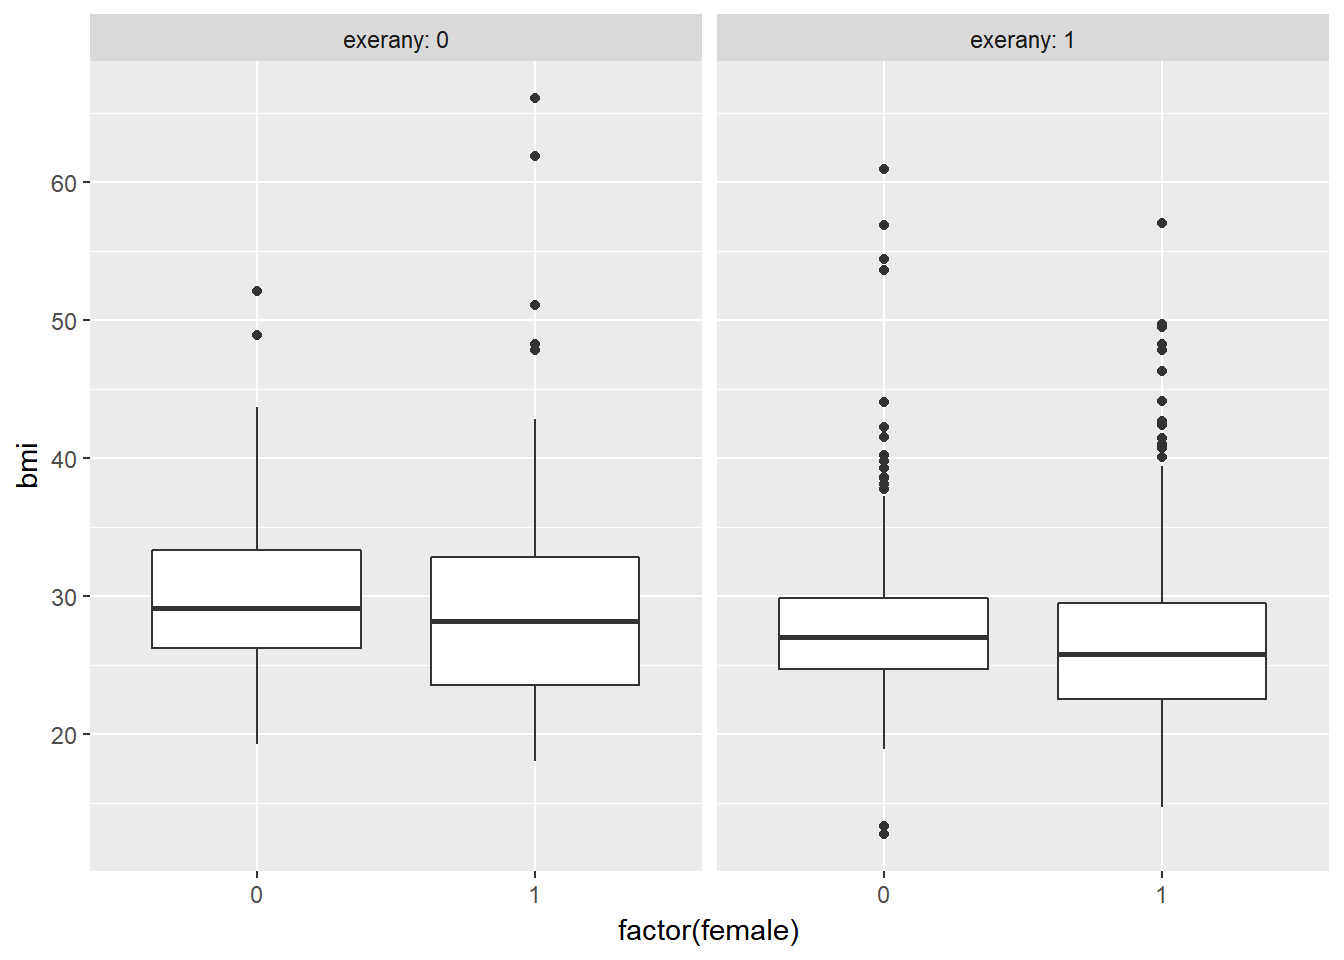
\includegraphics{bookdown-demo_files/figure-latex/c2_smartcle2_plot_bmi_box_by_female_exerany-1.pdf}

\begin{Shaded}
\begin{Highlighting}[]
\KeywordTok{ggplot}\NormalTok{(smartcle2, }\KeywordTok{aes}\NormalTok{(}\DataTypeTok{x =}\NormalTok{ female, }\DataTypeTok{y =}\NormalTok{ bmi))}\OperatorTok{+}
\StringTok{    }\KeywordTok{geom_point}\NormalTok{(}\DataTypeTok{size =} \DecValTok{3}\NormalTok{, }\DataTypeTok{alpha =} \FloatTok{0.2}\NormalTok{) }\OperatorTok{+}
\StringTok{    }\KeywordTok{theme_bw}\NormalTok{() }\OperatorTok{+}
\StringTok{    }\KeywordTok{facet_wrap}\NormalTok{(}\OperatorTok{~}\StringTok{ }\NormalTok{exerany, }\DataTypeTok{labeller =}\NormalTok{ label_both)}
\end{Highlighting}
\end{Shaded}

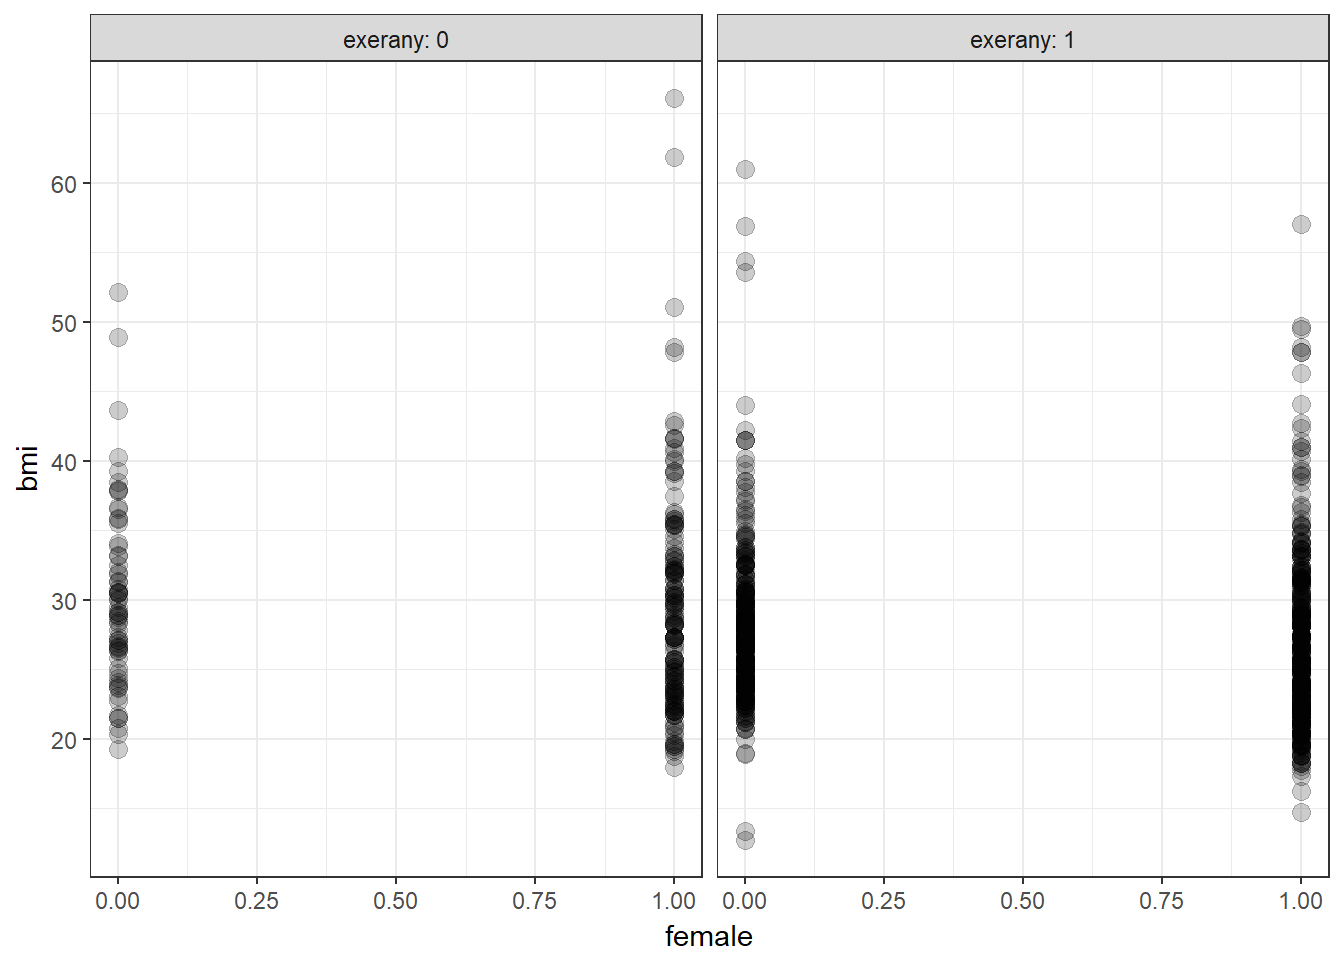
\includegraphics{bookdown-demo_files/figure-latex/c2_smartcle2_plot_bmi_points_by_female_exerany-1.pdf}

OK. Let's try fitting a model.

\begin{Shaded}
\begin{Highlighting}[]
\NormalTok{c2_m2 <-}\StringTok{ }\KeywordTok{lm}\NormalTok{(bmi }\OperatorTok{~}\StringTok{ }\NormalTok{female }\OperatorTok{+}\StringTok{ }\NormalTok{exerany, }\DataTypeTok{data =}\NormalTok{ smartcle2)}
\NormalTok{c2_m2}
\end{Highlighting}
\end{Shaded}

\begin{verbatim}

Call:
lm(formula = bmi ~ female + exerany, data = smartcle2)

Coefficients:
(Intercept)       female      exerany  
     30.334       -1.095       -2.384  
\end{verbatim}

This new model predicts only four predicted values:

\begin{itemize}
\tightlist
\item
  \texttt{bmi} = 30.334 if the subject is male and did not exercise (so
  \texttt{female} = 0 and \texttt{exerany} = 0)
\item
  \texttt{bmi} = 30.334 - 1.095 = 29.239 if the subject is female and
  did not exercise (\texttt{female} = 1 and \texttt{exerany} = 0)
\item
  \texttt{bmi} = 30.334 - 2.384 = 27.950 if the subject is male and
  exercised (so \texttt{female} = 0 and \texttt{exerany} = 1), and,
  finally
\item
  \texttt{bmi} = 30.334 - 1.095 - 2.384 = 26.855 if the subject is
  female and exercised (so both \texttt{female} and \texttt{exerany} =
  1).
\end{itemize}

For those who did not exercise, the model is:

\begin{itemize}
\tightlist
\item
  \texttt{bmi} = 30.334 - 1.095 \texttt{female}
\end{itemize}

and for those who did exercise, the model is:

\begin{itemize}
\tightlist
\item
  \texttt{bmi} = 27.95 - 1.095 \texttt{female}
\end{itemize}

Only the intercept of the \texttt{bmi-female} model changes depending on
\texttt{exerany}.

\begin{Shaded}
\begin{Highlighting}[]
\KeywordTok{summary}\NormalTok{(c2_m2)}
\end{Highlighting}
\end{Shaded}

\begin{verbatim}

Call:
lm(formula = bmi ~ female + exerany, data = smartcle2)

Residuals:
    Min      1Q  Median      3Q     Max 
-15.240  -4.091  -1.095   2.602  36.822 

Coefficients:
            Estimate Std. Error t value Pr(>|t|)    
(Intercept)  30.3335     0.5231   57.99  < 2e-16 ***
female       -1.0952     0.4262   -2.57   0.0103 *  
exerany      -2.3836     0.4965   -4.80 1.86e-06 ***
---
Signif. codes:  0 '***' 0.001 '**' 0.01 '*' 0.05 '.' 0.1 ' ' 1

Residual standard error: 6.239 on 893 degrees of freedom
Multiple R-squared:  0.02939,   Adjusted R-squared:  0.02722 
F-statistic: 13.52 on 2 and 893 DF,  p-value: 1.641e-06
\end{verbatim}

\begin{Shaded}
\begin{Highlighting}[]
\KeywordTok{confint}\NormalTok{(c2_m2)}
\end{Highlighting}
\end{Shaded}

\begin{verbatim}
                2.5 %     97.5 %
(Intercept) 29.306846 31.3602182
female      -1.931629 -0.2588299
exerany     -3.358156 -1.4090777
\end{verbatim}

The slopes of both \texttt{female} and \texttt{exerany} have confidence
intervals that are completely below zero, indicating that both
\texttt{female} sex and \texttt{exerany} appear to be associated with
reductions in \texttt{bmi}.

The R\textsuperscript{2} value suggests that just under 3\% of the
variation in \texttt{bmi} is accounted for by this ANOVA model.

In fact, this regression (on two binary indicator variables) is simply a
two-way ANOVA model without an interaction term.

\begin{Shaded}
\begin{Highlighting}[]
\KeywordTok{anova}\NormalTok{(c2_m2)}
\end{Highlighting}
\end{Shaded}

\begin{verbatim}
Analysis of Variance Table

Response: bmi
           Df Sum Sq Mean Sq F value    Pr(>F)    
female      1    156  155.61  3.9977   0.04586 *  
exerany     1    897  896.93 23.0435 1.856e-06 ***
Residuals 893  34759   38.92                      
---
Signif. codes:  0 '***' 0.001 '**' 0.01 '*' 0.05 '.' 0.1 ' ' 1
\end{verbatim}

\section{\texorpdfstring{\texttt{c2\_m3}: Adding the interaction term
(Two-way ANOVA with
interaction)}{c2\_m3: Adding the interaction term (Two-way ANOVA with interaction)}}\label{c2_m3-adding-the-interaction-term-two-way-anova-with-interaction}

Suppose we want to let the effect of \texttt{female} vary depending on
the \texttt{exerany} status. Then we need to incorporate an interaction
term in our model.

\begin{Shaded}
\begin{Highlighting}[]
\NormalTok{c2_m3 <-}\StringTok{ }\KeywordTok{lm}\NormalTok{(bmi }\OperatorTok{~}\StringTok{ }\NormalTok{female }\OperatorTok{*}\StringTok{ }\NormalTok{exerany, }\DataTypeTok{data =}\NormalTok{ smartcle2)}
\NormalTok{c2_m3}
\end{Highlighting}
\end{Shaded}

\begin{verbatim}

Call:
lm(formula = bmi ~ female * exerany, data = smartcle2)

Coefficients:
   (Intercept)          female         exerany  female:exerany  
       30.1359         -0.8104         -2.1450         -0.3592  
\end{verbatim}

So, for example, for a male who exercises, this model predicts

\begin{itemize}
\tightlist
\item
  \texttt{bmi} = 30.136 - 0.810 (0) - 2.145 (1) - 0.359 (0)(1) = 30.136
  - 2.145 = 27.991
\end{itemize}

And for a female who exercises, the model predicts

\begin{itemize}
\tightlist
\item
  \texttt{bmi} = 30.136 - 0.810 (1) - 2.145 (1) - 0.359 (1)(1) = 30.136
  - 0.810 - 2.145 - 0.359 = 26.822
\end{itemize}

For those who did not exercise, the model is:

\begin{itemize}
\tightlist
\item
  \texttt{bmi} = 30.136 - 0.81 \texttt{female}
\end{itemize}

But for those who did exercise, the model is:

\begin{itemize}
\tightlist
\item
  \texttt{bmi} = (30.136 - 2.145) + (-0.810 + (-0.359)) \texttt{female},
  or ,,,
\item
  \texttt{bmi} = 27.991 - 1.169 \texttt{female}
\end{itemize}

Now, both the slope and the intercept of the \texttt{bmi-female} model
change depending on \texttt{exerany}.

\begin{Shaded}
\begin{Highlighting}[]
\KeywordTok{summary}\NormalTok{(c2_m3)}
\end{Highlighting}
\end{Shaded}

\begin{verbatim}

Call:
lm(formula = bmi ~ female * exerany, data = smartcle2)

Residuals:
    Min      1Q  Median      3Q     Max 
-15.281  -4.101  -1.061   2.566  36.734 

Coefficients:
               Estimate Std. Error t value Pr(>|t|)    
(Intercept)     30.1359     0.7802  38.624   <2e-16 ***
female          -0.8104     0.9367  -0.865   0.3872    
exerany         -2.1450     0.8575  -2.501   0.0125 *  
female:exerany  -0.3592     1.0520  -0.341   0.7328    
---
Signif. codes:  0 '***' 0.001 '**' 0.01 '*' 0.05 '.' 0.1 ' ' 1

Residual standard error: 6.242 on 892 degrees of freedom
Multiple R-squared:  0.02952,   Adjusted R-squared:  0.02625 
F-statistic: 9.044 on 3 and 892 DF,  p-value: 6.669e-06
\end{verbatim}

\begin{Shaded}
\begin{Highlighting}[]
\KeywordTok{confint}\NormalTok{(c2_m3)}
\end{Highlighting}
\end{Shaded}

\begin{verbatim}
                   2.5 %     97.5 %
(Intercept)    28.604610 31.6672650
female         -2.648893  1.0280526
exerany        -3.827886 -0.4620407
female:exerany -2.423994  1.7055248
\end{verbatim}

In fact, this regression (on two binary indicator variables and a
product term) is simply a two-way ANOVA model with an interaction term.

\begin{Shaded}
\begin{Highlighting}[]
\KeywordTok{anova}\NormalTok{(c2_m3)}
\end{Highlighting}
\end{Shaded}

\begin{verbatim}
Analysis of Variance Table

Response: bmi
                Df Sum Sq Mean Sq F value    Pr(>F)    
female           1    156  155.61  3.9938   0.04597 *  
exerany          1    897  896.93 23.0207 1.878e-06 ***
female:exerany   1      5    4.54  0.1166   0.73283    
Residuals      892  34754   38.96                      
---
Signif. codes:  0 '***' 0.001 '**' 0.01 '*' 0.05 '.' 0.1 ' ' 1
\end{verbatim}

The interaction term doesn't change very much here. Its uncertainty
interval includes zero, and the overall model still accounts for just
under 3\% of the variation in \texttt{bmi}.

\section{\texorpdfstring{\texttt{c2\_m4}: Using \texttt{female} and
\texttt{sleephrs} in a model for
\texttt{bmi}}{c2\_m4: Using female and sleephrs in a model for bmi}}\label{c2_m4-using-female-and-sleephrs-in-a-model-for-bmi}

\begin{Shaded}
\begin{Highlighting}[]
\KeywordTok{ggplot}\NormalTok{(smartcle2, }\KeywordTok{aes}\NormalTok{(}\DataTypeTok{x =}\NormalTok{ sleephrs, }\DataTypeTok{y =}\NormalTok{ bmi, }\DataTypeTok{color =} \KeywordTok{factor}\NormalTok{(female))) }\OperatorTok{+}
\StringTok{    }\KeywordTok{geom_point}\NormalTok{() }\OperatorTok{+}\StringTok{ }
\StringTok{    }\KeywordTok{guides}\NormalTok{(}\DataTypeTok{col =} \OtherTok{FALSE}\NormalTok{) }\OperatorTok{+}
\StringTok{    }\KeywordTok{geom_smooth}\NormalTok{(}\DataTypeTok{method =} \StringTok{"lm"}\NormalTok{, }\DataTypeTok{se =} \OtherTok{FALSE}\NormalTok{) }\OperatorTok{+}
\StringTok{    }\KeywordTok{facet_wrap}\NormalTok{(}\OperatorTok{~}\StringTok{ }\NormalTok{female, }\DataTypeTok{labeller =}\NormalTok{ label_both) }
\end{Highlighting}
\end{Shaded}

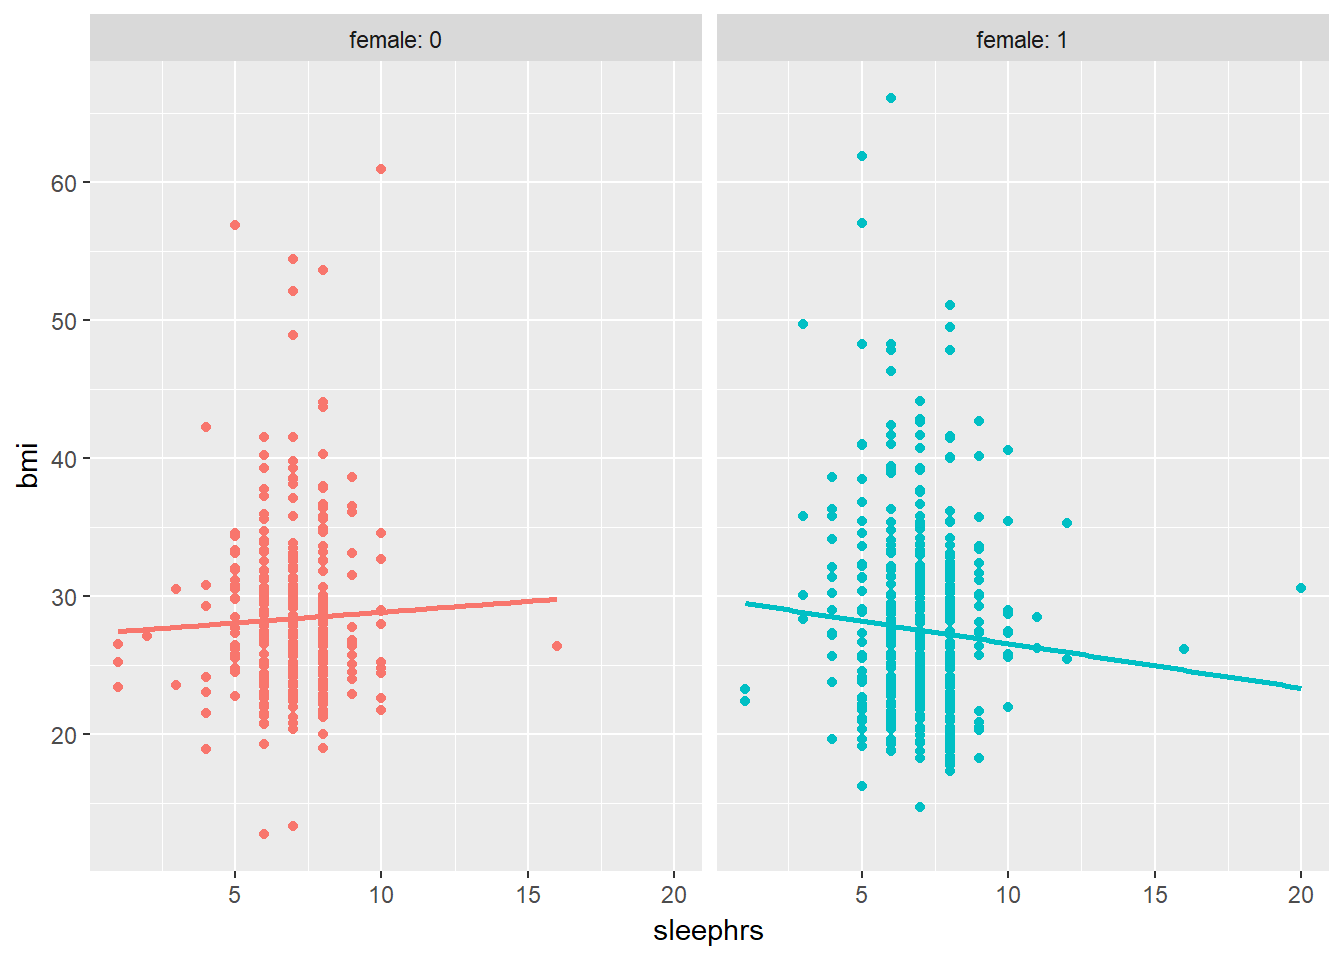
\includegraphics{bookdown-demo_files/figure-latex/graph_to_set_up_c2_m4-1.pdf}

Does the difference in slopes of \texttt{bmi} and \texttt{sleephrs} for
males and females appear to be substantial and important?

\begin{Shaded}
\begin{Highlighting}[]
\NormalTok{c2_m4 <-}\StringTok{ }\KeywordTok{lm}\NormalTok{(bmi }\OperatorTok{~}\StringTok{ }\NormalTok{female }\OperatorTok{*}\StringTok{ }\NormalTok{sleephrs, }\DataTypeTok{data =}\NormalTok{ smartcle2)}

\KeywordTok{summary}\NormalTok{(c2_m4)}
\end{Highlighting}
\end{Shaded}

\begin{verbatim}

Call:
lm(formula = bmi ~ female * sleephrs, data = smartcle2)

Residuals:
    Min      1Q  Median      3Q     Max 
-15.498  -4.179  -1.035   2.830  38.204 

Coefficients:
                Estimate Std. Error t value Pr(>|t|)    
(Intercept)      27.2661     1.6320  16.707   <2e-16 ***
female            2.5263     2.0975   1.204    0.229    
sleephrs          0.1569     0.2294   0.684    0.494    
female:sleephrs  -0.4797     0.2931  -1.636    0.102    
---
Signif. codes:  0 '***' 0.001 '**' 0.01 '*' 0.05 '.' 0.1 ' ' 1

Residual standard error: 6.31 on 892 degrees of freedom
Multiple R-squared:  0.008341,  Adjusted R-squared:  0.005006 
F-statistic: 2.501 on 3 and 892 DF,  p-value: 0.05818
\end{verbatim}

Does it seem as though the addition of \texttt{sleephrs} has improved
our model substantially over a model with \texttt{female} alone (which,
you recall, was \texttt{c2\_m1})?

Since the \texttt{c2\_m4} model contains the \texttt{c2\_m1} model's
predictors as a subset and the outcome is the same for each model, we
consider the models \emph{nested} and have some extra tools available to
compare them.

\begin{itemize}
\tightlist
\item
  I might start by looking at the basic summaries for each model.
\end{itemize}

\begin{Shaded}
\begin{Highlighting}[]
\KeywordTok{glance}\NormalTok{(c2_m4)}
\end{Highlighting}
\end{Shaded}

\begin{verbatim}
    r.squared adj.r.squared    sigma statistic    p.value df    logLik
1 0.008341404   0.005006229 6.309685   2.50104 0.05818038  4 -2919.873
       AIC      BIC deviance df.residual
1 5849.747 5873.736 35512.42         892
\end{verbatim}

\begin{Shaded}
\begin{Highlighting}[]
\KeywordTok{glance}\NormalTok{(c2_m1)}
\end{Highlighting}
\end{Shaded}

\begin{verbatim}
    r.squared adj.r.squared   sigma statistic    p.value df    logLik
1 0.004345169   0.003231461 6.31531  3.901534 0.04854928  2 -2921.675
      AIC      BIC deviance df.residual
1 5849.35 5863.744 35655.53         894
\end{verbatim}

\begin{itemize}
\tightlist
\item
  The R\textsuperscript{2} is twice as large for the model with
  \texttt{sleephrs}, but still very tiny.
\item
  The \emph{p} value for the global ANOVA test is actually less
  significant in \texttt{c2\_m4} than in \texttt{c2\_m1}.
\item
  Smaller AIC and smaller BIC statistics are more desirable. Here,
  there's little to choose from, but \texttt{c2\_m1} is a little better
  on each standard.
\item
  We might also consider a significance test by looking at an ANOVA
  model comparison. This is only appropriate because \texttt{c2\_m1} is
  nested in \texttt{c2\_m4}.
\end{itemize}

\begin{Shaded}
\begin{Highlighting}[]
\KeywordTok{anova}\NormalTok{(c2_m4, c2_m1)}
\end{Highlighting}
\end{Shaded}

\begin{verbatim}
Analysis of Variance Table

Model 1: bmi ~ female * sleephrs
Model 2: bmi ~ female
  Res.Df   RSS Df Sum of Sq      F Pr(>F)
1    892 35512                           
2    894 35656 -2   -143.11 1.7973 0.1663
\end{verbatim}

The addition of the \texttt{sleephrs} term picked up 143 in the sum of
squares column, at a cost of two degrees of freedom, yielding a \emph{p}
value of 0.166, suggesting that this isn't a significant improvement
over the model that just did a t-test on \texttt{female}.

\section{Making Predictions with a Linear Regression
Model}\label{making-predictions-with-a-linear-regression-model}

Recall model 4, which yields predictions for body mass index on the
basis of the main effects of sex (\texttt{female}) and hours of sleep
(\texttt{sleephrs}) and their interaction.

\begin{Shaded}
\begin{Highlighting}[]
\NormalTok{c2_m4}
\end{Highlighting}
\end{Shaded}

\begin{verbatim}

Call:
lm(formula = bmi ~ female * sleephrs, data = smartcle2)

Coefficients:
    (Intercept)           female         sleephrs  female:sleephrs  
        27.2661           2.5263           0.1569          -0.4797  
\end{verbatim}

\subsection{Fitting an Individual Prediction and 95\% Prediction
Interval}\label{fitting-an-individual-prediction-and-95-prediction-interval}

What do we predict for the \texttt{bmi} of a subject who is
\texttt{female} and gets 8 hours of sleep per night?

\begin{Shaded}
\begin{Highlighting}[]
\NormalTok{c2_new1 <-}\StringTok{ }\KeywordTok{data_frame}\NormalTok{(}\DataTypeTok{female =} \DecValTok{1}\NormalTok{, }\DataTypeTok{sleephrs =} \DecValTok{8}\NormalTok{)}
\KeywordTok{predict}\NormalTok{(c2_m4, }\DataTypeTok{newdata =}\NormalTok{ c2_new1, }\DataTypeTok{interval =} \StringTok{"prediction"}\NormalTok{, }\DataTypeTok{level =} \FloatTok{0.95}\NormalTok{)}
\end{Highlighting}
\end{Shaded}

\begin{verbatim}
       fit     lwr     upr
1 27.21065 14.8107 39.6106
\end{verbatim}

The predicted \texttt{bmi} for this new subject is 27.61. The prediction
interval shows the bounds of a 95\% uncertainty interval for a predicted
\texttt{bmi} for an individual female subject who gets 8 hours of sleep
on average per evening. From the \texttt{predict} function applied to a
linear model, we can get the prediction intervals for any new data
points in this manner.

\subsection{Confidence Interval for an Average
Prediction}\label{confidence-interval-for-an-average-prediction}

\begin{itemize}
\tightlist
\item
  What do we predict for the \textbf{average body mass index of a
  population of subjects} who are female and sleep for 8 hours?
\end{itemize}

\begin{Shaded}
\begin{Highlighting}[]
\KeywordTok{predict}\NormalTok{(c2_m4, }\DataTypeTok{newdata =}\NormalTok{ c2_new1, }\DataTypeTok{interval =} \StringTok{"confidence"}\NormalTok{, }\DataTypeTok{level =} \FloatTok{0.95}\NormalTok{)}
\end{Highlighting}
\end{Shaded}

\begin{verbatim}
       fit      lwr      upr
1 27.21065 26.57328 27.84801
\end{verbatim}

\begin{itemize}
\tightlist
\item
  How does this result compare to the prediction interval?
\end{itemize}

\subsection{Fitting Multiple Individual Predictions to New
Data}\label{fitting-multiple-individual-predictions-to-new-data}

\begin{itemize}
\tightlist
\item
  How does our prediction change for a respondent if they instead get 7,
  or 9 hours of sleep? What if they are male, instead of female?
\end{itemize}

\begin{Shaded}
\begin{Highlighting}[]
\NormalTok{c2_new2 <-}\StringTok{ }\KeywordTok{data_frame}\NormalTok{(}\DataTypeTok{subjectid =} \DecValTok{1001}\OperatorTok{:}\DecValTok{1006}\NormalTok{, }\DataTypeTok{female =} \KeywordTok{c}\NormalTok{(}\DecValTok{1}\NormalTok{, }\DecValTok{1}\NormalTok{, }\DecValTok{1}\NormalTok{, }\DecValTok{0}\NormalTok{, }\DecValTok{0}\NormalTok{, }\DecValTok{0}\NormalTok{), }\DataTypeTok{sleephrs =} \KeywordTok{c}\NormalTok{(}\DecValTok{7}\NormalTok{, }\DecValTok{8}\NormalTok{, }\DecValTok{9}\NormalTok{, }\DecValTok{7}\NormalTok{, }\DecValTok{8}\NormalTok{, }\DecValTok{9}\NormalTok{))}
\NormalTok{pred2 <-}\StringTok{ }\KeywordTok{predict}\NormalTok{(c2_m4, }\DataTypeTok{newdata =}\NormalTok{ c2_new2, }\DataTypeTok{interval =} \StringTok{"prediction"}\NormalTok{, }\DataTypeTok{level =} \FloatTok{0.95}\NormalTok{) }\OperatorTok\StringTok{ }\NormalTok{tbl_df}

\NormalTok{result2 <-}\StringTok{ }\KeywordTok{bind_cols}\NormalTok{(c2_new2, pred2)}
\NormalTok{result2}
\end{Highlighting}
\end{Shaded}

\begin{verbatim}
# A tibble: 6 x 6
  subjectid female sleephrs   fit   lwr   upr
      <int>  <dbl>    <dbl> <dbl> <dbl> <dbl>
1      1001   1.00     7.00  27.5  15.1  39.9
2      1002   1.00     8.00  27.2  14.8  39.6
3      1003   1.00     9.00  26.9  14.5  39.3
4      1004   0        7.00  28.4  16.0  40.8
5      1005   0        8.00  28.5  16.1  40.9
6      1006   0        9.00  28.7  16.2  41.1
\end{verbatim}

The \texttt{result2} tibble contains predictions for each scenario.

\begin{itemize}
\tightlist
\item
  Which has a bigger impact on these predictions and prediction
  intervals? A one category change in \texttt{female} or a one hour
  change in \texttt{sleephrs}?
\end{itemize}

\subsection{Simulation to represent predictive uncertainty in Model
4}\label{simulation-to-represent-predictive-uncertainty-in-model-4}

Suppose we want to predict the \texttt{bmi} of a female subject who
sleeps for eight hours per night. As we have seen, we can do this
automatically for a linear model like this one, using the
\texttt{predict} function applied to the linear model, but a simulation
prediction can also be done. Recall the detail of \texttt{c2\_m4}:

\begin{Shaded}
\begin{Highlighting}[]
\NormalTok{c2_m4}
\end{Highlighting}
\end{Shaded}

\begin{verbatim}

Call:
lm(formula = bmi ~ female * sleephrs, data = smartcle2)

Coefficients:
    (Intercept)           female         sleephrs  female:sleephrs  
        27.2661           2.5263           0.1569          -0.4797  
\end{verbatim}

\begin{Shaded}
\begin{Highlighting}[]
\KeywordTok{glance}\NormalTok{(c2_m4)}
\end{Highlighting}
\end{Shaded}

\begin{verbatim}
    r.squared adj.r.squared    sigma statistic    p.value df    logLik
1 0.008341404   0.005006229 6.309685   2.50104 0.05818038  4 -2919.873
       AIC      BIC deviance df.residual
1 5849.747 5873.736 35512.42         892
\end{verbatim}

We see that the residual standard error for our \texttt{bmi} predictions
with this model is 6.31.

For a female respondent sleeping eight hours, recall that our point
estimate (predicted value) of \texttt{bmi} is 27.21

\begin{Shaded}
\begin{Highlighting}[]
\KeywordTok{predict}\NormalTok{(c2_m4, }\DataTypeTok{newdata =}\NormalTok{ c2_new1, }\DataTypeTok{interval =} \StringTok{"prediction"}\NormalTok{, }\DataTypeTok{level =} \FloatTok{0.95}\NormalTok{)}
\end{Highlighting}
\end{Shaded}

\begin{verbatim}
       fit     lwr     upr
1 27.21065 14.8107 39.6106
\end{verbatim}

The standard deviation is 6.31, so we could summarize the predictive
distribution with a command that tells R to draw 1000 random numbers
from a normal distribution with mean 27.21 and standard deviation 6.31.
Let's summarize that and get a quick picture.

\begin{Shaded}
\begin{Highlighting}[]
\KeywordTok{set.seed}\NormalTok{(}\DecValTok{432094}\NormalTok{)}
\NormalTok{pred.sim <-}\StringTok{ }\KeywordTok{rnorm}\NormalTok{(}\DecValTok{1000}\NormalTok{, }\FloatTok{27.21}\NormalTok{, }\FloatTok{6.31}\NormalTok{)}
\KeywordTok{hist}\NormalTok{(pred.sim, }\DataTypeTok{col =} \StringTok{"royalblue"}\NormalTok{)}
\end{Highlighting}
\end{Shaded}

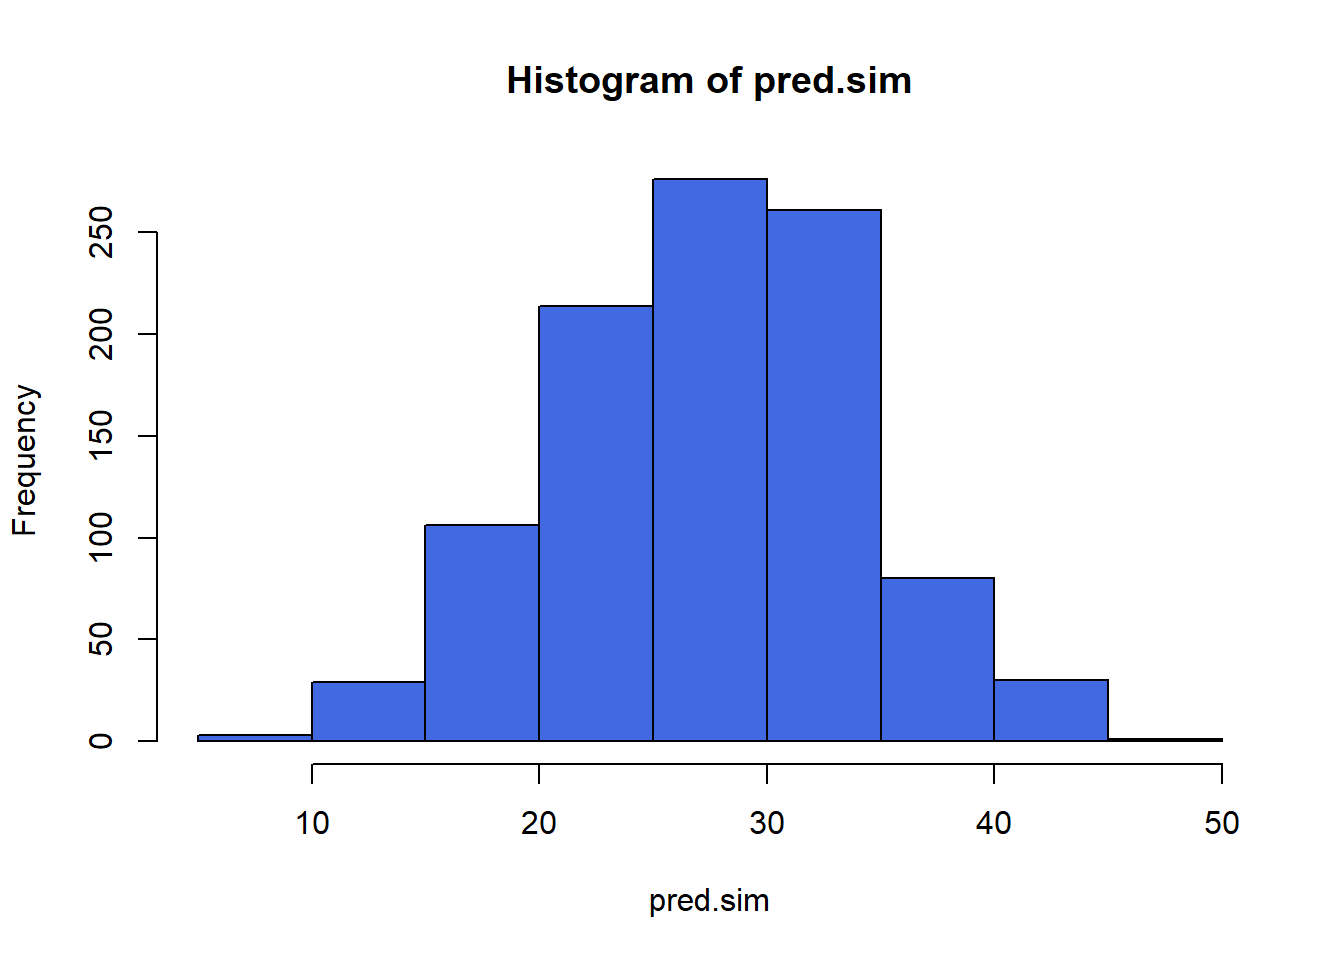
\includegraphics{bookdown-demo_files/figure-latex/unnamed-chunk-10-1.pdf}

\begin{Shaded}
\begin{Highlighting}[]
\KeywordTok{mean}\NormalTok{(pred.sim)}
\end{Highlighting}
\end{Shaded}

\begin{verbatim}
[1] 27.41856
\end{verbatim}

\begin{Shaded}
\begin{Highlighting}[]
\KeywordTok{quantile}\NormalTok{(pred.sim, }\KeywordTok{c}\NormalTok{(}\FloatTok{0.025}\NormalTok{, }\FloatTok{0.975}\NormalTok{))}
\end{Highlighting}
\end{Shaded}

\begin{verbatim}
    2.5%    97.5% 
14.48487 40.16778 
\end{verbatim}

How do these results compare to the prediction interval of (14.81,
39.61) that we generated earlier?

\section{Centering the model}\label{centering-the-model}

Our model \texttt{c2\_m4} has four predictors (the constant,
\texttt{sleephrs}, \texttt{female} and their interaction) but just two
inputs (\texttt{female} and \texttt{sleephrs}.) If we \textbf{center}
the quantitative input \texttt{sleephrs} before building the model, we
get a more interpretable interaction term.

\begin{Shaded}
\begin{Highlighting}[]
\NormalTok{smartcle2_c <-}\StringTok{ }\NormalTok{smartcle2 }\OperatorTok
\StringTok{    }\KeywordTok{mutate}\NormalTok{(}\DataTypeTok{sleephrs_c =}\NormalTok{ sleephrs }\OperatorTok{-}\StringTok{ }\KeywordTok{mean}\NormalTok{(sleephrs))}

\NormalTok{c2_m4_c <-}\StringTok{ }\KeywordTok{lm}\NormalTok{(bmi }\OperatorTok{~}\StringTok{ }\NormalTok{female }\OperatorTok{*}\StringTok{ }\NormalTok{sleephrs_c, }\DataTypeTok{data =}\NormalTok{ smartcle2_c)}

\KeywordTok{summary}\NormalTok{(c2_m4_c)}
\end{Highlighting}
\end{Shaded}

\begin{verbatim}

Call:
lm(formula = bmi ~ female * sleephrs_c, data = smartcle2_c)

Residuals:
    Min      1Q  Median      3Q     Max 
-15.498  -4.179  -1.035   2.830  38.204 

Coefficients:
                  Estimate Std. Error t value Pr(>|t|)    
(Intercept)        28.3681     0.3274  86.658   <2e-16 ***
female             -0.8420     0.4280  -1.967   0.0495 *  
sleephrs_c          0.1569     0.2294   0.684   0.4940    
female:sleephrs_c  -0.4797     0.2931  -1.636   0.1021    
---
Signif. codes:  0 '***' 0.001 '**' 0.01 '*' 0.05 '.' 0.1 ' ' 1

Residual standard error: 6.31 on 892 degrees of freedom
Multiple R-squared:  0.008341,  Adjusted R-squared:  0.005006 
F-statistic: 2.501 on 3 and 892 DF,  p-value: 0.05818
\end{verbatim}

What has changed as compared to the original \texttt{c2\_m4}?

\begin{itemize}
\tightlist
\item
  Our original model was \texttt{bmi} = 27.26 + 2.53 \texttt{female} +
  0.16 \texttt{sleephrs} - 0.48 \texttt{female} x \texttt{sleephrs}
\item
  Our new model is \texttt{bmi} = 28.37 - 0.84 \texttt{female} + 0.16
  centered \texttt{sleephrs} - 0.48 \texttt{female} x centered
  \texttt{sleephrs}.
\end{itemize}

So our new model on centered data is:

\begin{itemize}
\tightlist
\item
  28.37 + 0.16 centered \texttt{sleephrs\_c} for male subjects, and
\item
  (28.37 - 0.84) + (0.16 - 0.48) centered \texttt{sleephrs\_c}, or 27.53
  - 0.32 centered \texttt{sleephrs\_c} for female subjects.
\end{itemize}

In our new (centered \texttt{sleephrs\_c}) model,

\begin{itemize}
\tightlist
\item
  the main effect of \texttt{female} now corresponds to a predictive
  difference (female - male) in \texttt{bmi} with \texttt{sleephrs} at
  its mean value, 7.02 hours,
\item
  the intercept term is now the predicted \texttt{bmi} for a male
  respondent who sleeps an average number of hours, and
\item
  the product term corresponds to the change in the slope of centered
  \texttt{sleephrs\_c} on \texttt{bmi} for a female rather than a male
  subject, while
\item
  the residual standard deviation and the R-squared values remain
  unchanged from the model before centering.
\end{itemize}

\subsection{\texorpdfstring{Plot of Model 4 on Centered
\texttt{sleephrs}:
\texttt{c2\_m4\_c}}{Plot of Model 4 on Centered sleephrs: c2\_m4\_c}}\label{plot-of-model-4-on-centered-sleephrs-c2_m4_c}

\begin{Shaded}
\begin{Highlighting}[]
\KeywordTok{ggplot}\NormalTok{(smartcle2_c, }\KeywordTok{aes}\NormalTok{(}\DataTypeTok{x =}\NormalTok{ sleephrs_c, }\DataTypeTok{y =}\NormalTok{ bmi, }\DataTypeTok{group =}\NormalTok{ female, }\DataTypeTok{col =} \KeywordTok{factor}\NormalTok{(female))) }\OperatorTok{+}
\StringTok{    }\KeywordTok{geom_point}\NormalTok{(}\DataTypeTok{alpha =} \FloatTok{0.5}\NormalTok{, }\DataTypeTok{size =} \DecValTok{2}\NormalTok{) }\OperatorTok{+}
\StringTok{    }\KeywordTok{geom_smooth}\NormalTok{(}\DataTypeTok{method =} \StringTok{"lm"}\NormalTok{, }\DataTypeTok{se =} \OtherTok{FALSE}\NormalTok{) }\OperatorTok{+}
\StringTok{    }\KeywordTok{guides}\NormalTok{(}\DataTypeTok{color =} \OtherTok{FALSE}\NormalTok{) }\OperatorTok{+}
\StringTok{    }\KeywordTok{labs}\NormalTok{(}\DataTypeTok{x =} \StringTok{"Sleep Hours, centered"}\NormalTok{, }\DataTypeTok{y =} \StringTok{"Body Mass Index"}\NormalTok{,}
         \DataTypeTok{title =} \StringTok{"Model `c2_m4` on centered data"}\NormalTok{) }\OperatorTok{+}
\StringTok{    }\KeywordTok{facet_wrap}\NormalTok{(}\OperatorTok{~}\StringTok{ }\NormalTok{female, }\DataTypeTok{labeller =}\NormalTok{ label_both)}
\end{Highlighting}
\end{Shaded}

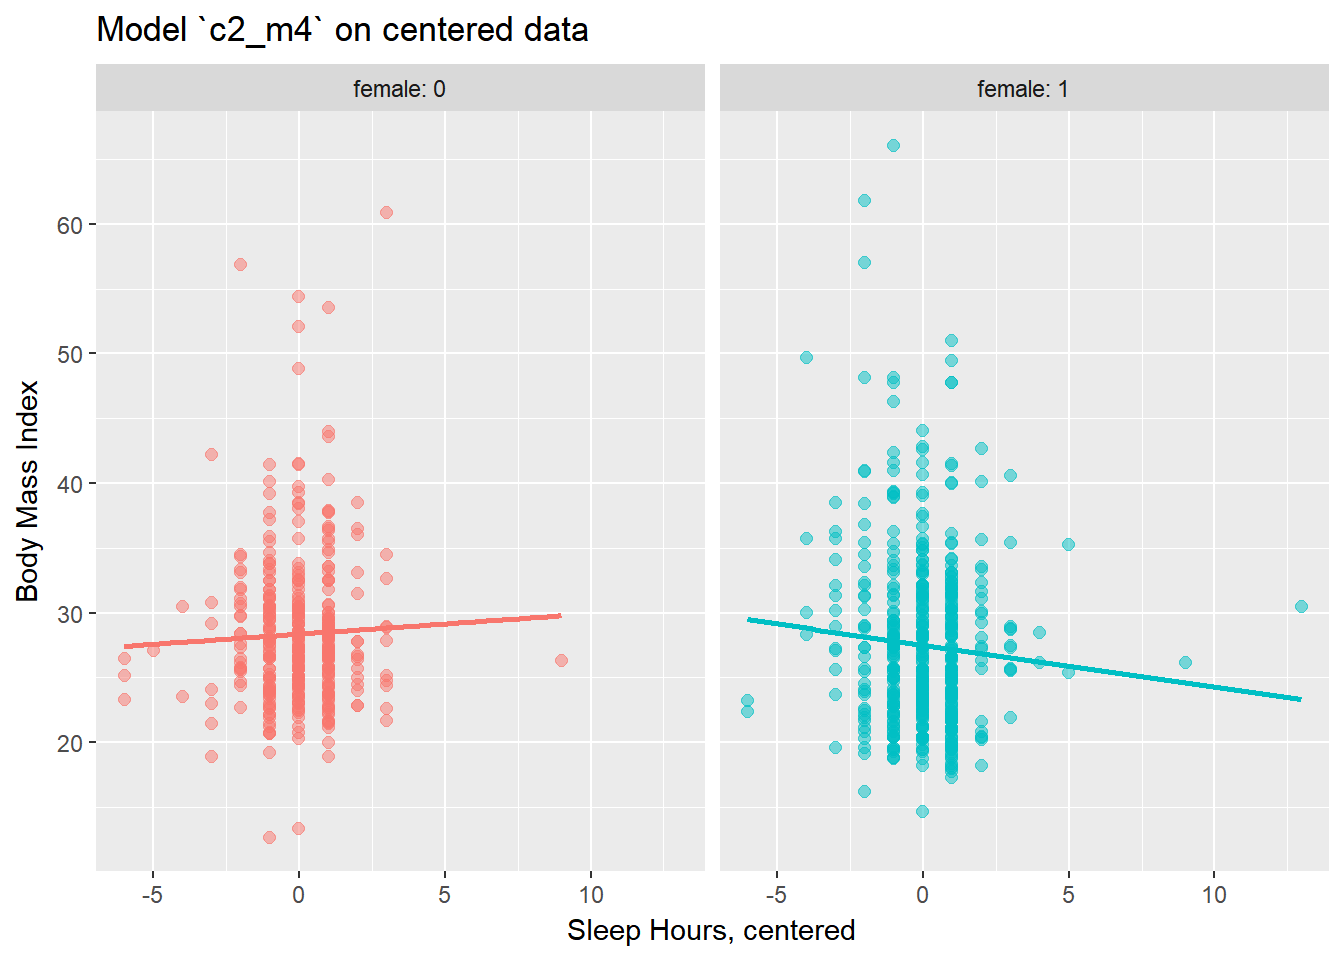
\includegraphics{bookdown-demo_files/figure-latex/unnamed-chunk-12-1.pdf}

\section{Rescaling an input by subtracting the mean and dividing by 2
standard
deviations}\label{rescaling-an-input-by-subtracting-the-mean-and-dividing-by-2-standard-deviations}

Centering helped us interpret the main effects in the regression, but it
still leaves a scaling problem.

\begin{itemize}
\tightlist
\item
  The \texttt{female} coefficient estimate is much larger than that of
  \texttt{sleephrs}, but this is misleading, considering that we are
  comparing the complete change in one variable (sex = female or not) to
  a 1-hour change in average sleep.
\item
  \citet{GelmanHill2007} recommend all continuous predictors be scaled
  by dividing by 2 standard deviations, so that:

  \begin{itemize}
  \tightlist
  \item
    a 1-unit change in the rescaled predictor corresponds to a change
    from 1 standard deviation below the mean, to 1 standard deviation
    above.
  \item
    an unscaled binary (1/0) predictor with 50\% probability of
    occurring will be exactly comparable to a rescaled continuous
    predictor done in this way.
  \end{itemize}
\end{itemize}

\begin{Shaded}
\begin{Highlighting}[]
\NormalTok{smartcle2_rescale <-}\StringTok{ }\NormalTok{smartcle2 }\OperatorTok
\StringTok{    }\KeywordTok{mutate}\NormalTok{(}\DataTypeTok{sleephrs_z =}\NormalTok{ (sleephrs }\OperatorTok{-}\StringTok{ }\KeywordTok{mean}\NormalTok{(sleephrs))}\OperatorTok{/}\NormalTok{(}\DecValTok{2}\OperatorTok{*}\KeywordTok{sd}\NormalTok{(sleephrs)))}
\end{Highlighting}
\end{Shaded}

\subsection{\texorpdfstring{Refitting model \texttt{c2\_m4} to the
rescaled
data}{Refitting model c2\_m4 to the rescaled data}}\label{refitting-model-c2_m4-to-the-rescaled-data}

\begin{Shaded}
\begin{Highlighting}[]
\NormalTok{c2_m4_z <-}\StringTok{ }\KeywordTok{lm}\NormalTok{(bmi }\OperatorTok{~}\StringTok{ }\NormalTok{female }\OperatorTok{*}\StringTok{ }\NormalTok{sleephrs_z, }\DataTypeTok{data =}\NormalTok{ smartcle2_rescale)}

\KeywordTok{summary}\NormalTok{(c2_m4_z)}
\end{Highlighting}
\end{Shaded}

\begin{verbatim}

Call:
lm(formula = bmi ~ female * sleephrs_z, data = smartcle2_rescale)

Residuals:
    Min      1Q  Median      3Q     Max 
-15.498  -4.179  -1.035   2.830  38.204 

Coefficients:
                  Estimate Std. Error t value Pr(>|t|)    
(Intercept)        28.3681     0.3274  86.658   <2e-16 ***
female             -0.8420     0.4280  -1.967   0.0495 *  
sleephrs_z          0.4637     0.6778   0.684   0.4940    
female:sleephrs_z  -1.4173     0.8661  -1.636   0.1021    
---
Signif. codes:  0 '***' 0.001 '**' 0.01 '*' 0.05 '.' 0.1 ' ' 1

Residual standard error: 6.31 on 892 degrees of freedom
Multiple R-squared:  0.008341,  Adjusted R-squared:  0.005006 
F-statistic: 2.501 on 3 and 892 DF,  p-value: 0.05818
\end{verbatim}

\subsection{Interpreting the model on rescaled
data}\label{interpreting-the-model-on-rescaled-data}

What has changed as compared to the original \texttt{c2\_m4}?

\begin{itemize}
\tightlist
\item
  Our original model was \texttt{bmi} = 27.26 + 2.53 \texttt{female} +
  0.16 \texttt{sleephrs} - 0.48 \texttt{female} x \texttt{sleephrs}
\item
  Our model on centered \texttt{sleephrs} was \texttt{bmi} = 28.37 -
  0.84 \texttt{female} + 0.16 centered \texttt{sleephrs\_c} - 0.48
  \texttt{female} x centered \texttt{sleephrs\_c}.
\item
  Our new model on rescaled \texttt{sleephrs} is \texttt{bmi} = 28.37 -
  0.84 \texttt{female} + 0.46 rescaled \texttt{sleephrs\_z} - 1.42
  \texttt{female} x rescaled \texttt{sleephrs\_z}.
\end{itemize}

So our rescaled model is:

\begin{itemize}
\tightlist
\item
  28.37 + 0.46 rescaled \texttt{sleephrs\_z} for male subjects, and
\item
  (28.37 - 0.84) + (0.46 - 1.42) rescaled \texttt{sleephrs\_z}, or 27.53
  - 0.96 rescaled \texttt{sleephrs\_z} for female subjects.
\end{itemize}

In this new rescaled (\texttt{sleephrs\_z}) model, then,

\begin{itemize}
\tightlist
\item
  the main effect of \texttt{female}, -0.84, still corresponds to a
  predictive difference (female - male) in \texttt{bmi} with
  \texttt{sleephrs} at its mean value, 7.02 hours,
\item
  the intercept term is still the predicted \texttt{bmi} for a male
  respondent who sleeps an average number of hours, and
\item
  the residual standard deviation and the R-squared values remain
  unchanged,
\end{itemize}

as before, but now we also have that:

\begin{itemize}
\tightlist
\item
  the coefficient of \texttt{sleephrs\_z} indicates the predictive
  difference in \texttt{bmi} associated with a change in
  \texttt{sleephrs} of 2 standard deviations (from one standard
  deviation below the mean of 7.02 to one standard deviation above
  7.02.)

  \begin{itemize}
  \tightlist
  \item
    Since the standard deviation of \texttt{sleephrs} is 1.48, this
    corresponds to a change from 5.54 hours per night to 8.50 hours per
    night.
  \end{itemize}
\item
  the coefficient of the product term (-1.42) corresponds to the change
  in the coefficient of \texttt{sleephrs\_z} for females as compared to
  males.
\end{itemize}

\subsection{Plot of model on rescaled
data}\label{plot-of-model-on-rescaled-data}

\begin{Shaded}
\begin{Highlighting}[]
\KeywordTok{ggplot}\NormalTok{(smartcle2_rescale, }\KeywordTok{aes}\NormalTok{(}\DataTypeTok{x =}\NormalTok{ sleephrs_z, }\DataTypeTok{y =}\NormalTok{ bmi, }
                              \DataTypeTok{group =}\NormalTok{ female, }\DataTypeTok{col =} \KeywordTok{factor}\NormalTok{(female))) }\OperatorTok{+}
\StringTok{    }\KeywordTok{geom_point}\NormalTok{(}\DataTypeTok{alpha =} \FloatTok{0.5}\NormalTok{) }\OperatorTok{+}
\StringTok{    }\KeywordTok{geom_smooth}\NormalTok{(}\DataTypeTok{method =} \StringTok{"lm"}\NormalTok{, }\DataTypeTok{size =} \FloatTok{1.5}\NormalTok{) }\OperatorTok{+}
\StringTok{    }\KeywordTok{scale_color_discrete}\NormalTok{(}\DataTypeTok{name =} \StringTok{"Is subject female?"}\NormalTok{) }\OperatorTok{+}
\StringTok{    }\KeywordTok{labs}\NormalTok{(}\DataTypeTok{x =} \StringTok{"Sleep Hours, standardized (2 sd)"}\NormalTok{, }\DataTypeTok{y =} \StringTok{"Body Mass Index"}\NormalTok{,}
         \DataTypeTok{title =} \StringTok{"Model `c2_m4_z` on rescaled data"}\NormalTok{)}
\end{Highlighting}
\end{Shaded}

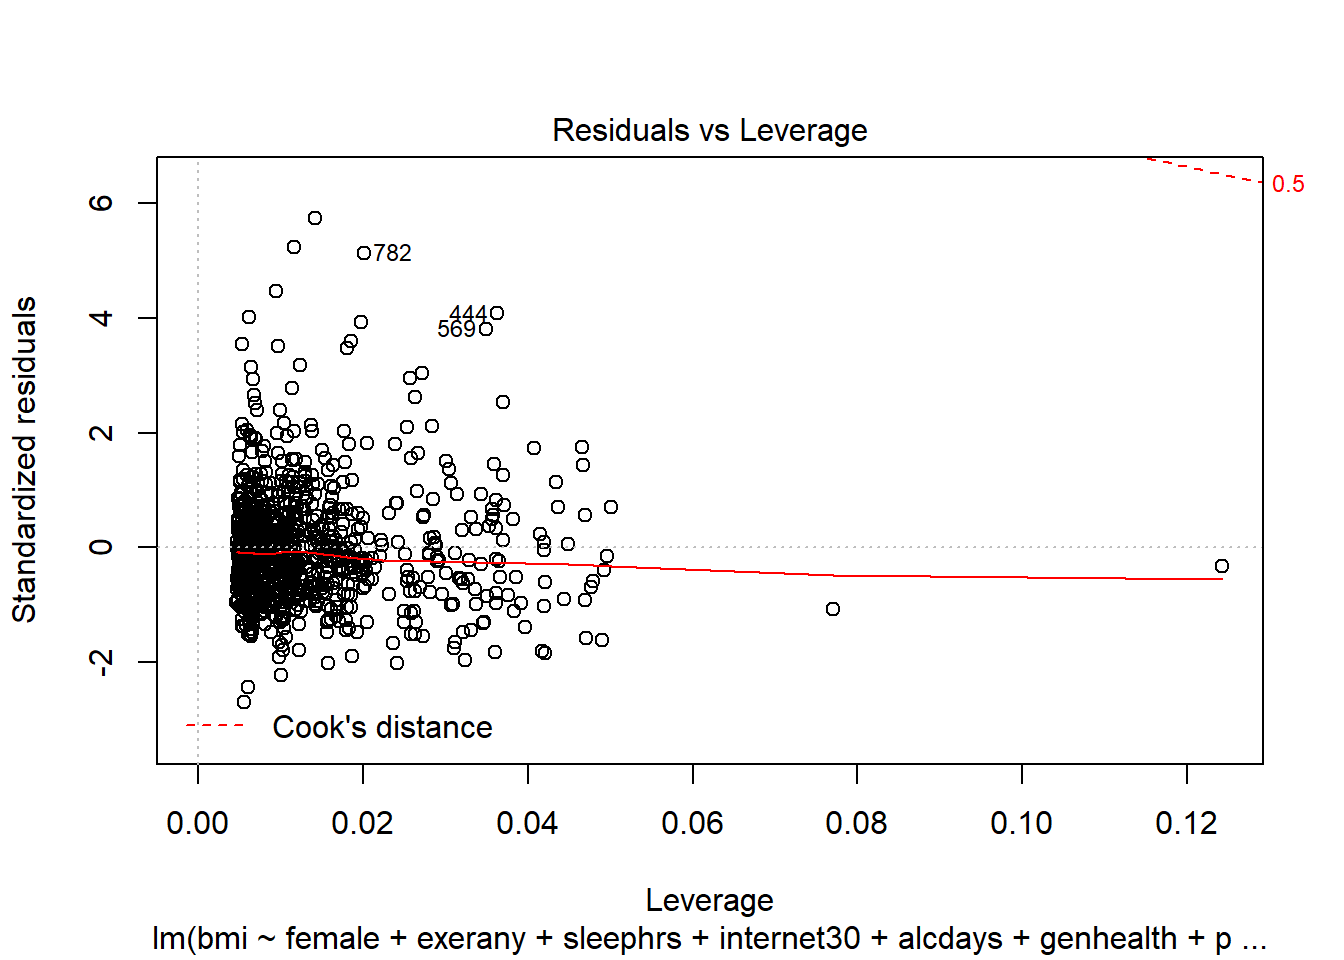
\includegraphics{bookdown-demo_files/figure-latex/unnamed-chunk-14-1.pdf}

\section{\texorpdfstring{\texttt{c2\_m5}: What if we add more
variables?}{c2\_m5: What if we add more variables?}}\label{c2_m5-what-if-we-add-more-variables}

We can boost our R\textsuperscript{2} a bit, to over 5\%, by adding in
two new variables, related to whether or not the subject (in the past 30
days) used the internet, and on how many days the subject drank
alcoholic beverages.

\begin{Shaded}
\begin{Highlighting}[]
\NormalTok{c2_m5 <-}\StringTok{ }\KeywordTok{lm}\NormalTok{(bmi }\OperatorTok{~}\StringTok{ }\NormalTok{female }\OperatorTok{+}\StringTok{ }\NormalTok{exerany }\OperatorTok{+}\StringTok{ }\NormalTok{sleephrs }\OperatorTok{+}\StringTok{ }\NormalTok{internet30 }\OperatorTok{+}\StringTok{ }\NormalTok{alcdays,}
         \DataTypeTok{data =}\NormalTok{ smartcle2)}
\KeywordTok{summary}\NormalTok{(c2_m5)}
\end{Highlighting}
\end{Shaded}

\begin{verbatim}

Call:
lm(formula = bmi ~ female + exerany + sleephrs + internet30 + 
    alcdays, data = smartcle2)

Residuals:
    Min      1Q  Median      3Q     Max 
-16.147  -3.997  -0.856   2.487  35.965 

Coefficients:
            Estimate Std. Error t value Pr(>|t|)    
(Intercept) 30.84066    1.18458  26.035  < 2e-16 ***
female      -1.28801    0.42805  -3.009   0.0027 ** 
exerany     -2.42161    0.49853  -4.858 1.40e-06 ***
sleephrs    -0.14118    0.13988  -1.009   0.3131    
internet30   1.38916    0.54252   2.561   0.0106 *  
alcdays     -0.10460    0.02595  -4.030 6.04e-05 ***
---
Signif. codes:  0 '***' 0.001 '**' 0.01 '*' 0.05 '.' 0.1 ' ' 1

Residual standard error: 6.174 on 890 degrees of freedom
Multiple R-squared:  0.05258,   Adjusted R-squared:  0.04726 
F-statistic: 9.879 on 5 and 890 DF,  p-value: 3.304e-09
\end{verbatim}

\begin{enumerate}
\def\labelenumi{\arabic{enumi}.}
\tightlist
\item
  Here's the ANOVA for this model. What can we study with this?
\end{enumerate}

\begin{Shaded}
\begin{Highlighting}[]
\KeywordTok{anova}\NormalTok{(c2_m5)}
\end{Highlighting}
\end{Shaded}

\begin{verbatim}
Analysis of Variance Table

Response: bmi
            Df Sum Sq Mean Sq F value    Pr(>F)    
female       1    156  155.61  4.0818   0.04365 *  
exerany      1    897  896.93 23.5283 1.453e-06 ***
sleephrs     1     33   32.90  0.8631   0.35313    
internet30   1    178  178.33  4.6779   0.03082 *  
alcdays      1    619  619.26 16.2443 6.044e-05 ***
Residuals  890  33928   38.12                      
---
Signif. codes:  0 '***' 0.001 '**' 0.01 '*' 0.05 '.' 0.1 ' ' 1
\end{verbatim}

\begin{enumerate}
\def\labelenumi{\arabic{enumi}.}
\setcounter{enumi}{1}
\tightlist
\item
  Consider the revised output below. Now what can we study?
\end{enumerate}

\begin{Shaded}
\begin{Highlighting}[]
\KeywordTok{anova}\NormalTok{(}\KeywordTok{lm}\NormalTok{(bmi }\OperatorTok{~}\StringTok{ }\NormalTok{exerany }\OperatorTok{+}\StringTok{ }\NormalTok{internet30 }\OperatorTok{+}\StringTok{ }\NormalTok{alcdays }\OperatorTok{+}\StringTok{ }\NormalTok{female }\OperatorTok{+}\StringTok{ }\NormalTok{sleephrs,}
         \DataTypeTok{data =}\NormalTok{ smartcle2))}
\end{Highlighting}
\end{Shaded}

\begin{verbatim}
Analysis of Variance Table

Response: bmi
            Df Sum Sq Mean Sq F value    Pr(>F)    
exerany      1    795  795.46 20.8664 5.618e-06 ***
internet30   1    212  211.95  5.5599 0.0185925 *  
alcdays      1    486  486.03 12.7496 0.0003752 ***
female       1    351  350.75  9.2010 0.0024891 ** 
sleephrs     1     39   38.83  1.0186 0.3131176    
Residuals  890  33928   38.12                      
---
Signif. codes:  0 '***' 0.001 '**' 0.01 '*' 0.05 '.' 0.1 ' ' 1
\end{verbatim}

\begin{enumerate}
\def\labelenumi{\arabic{enumi}.}
\setcounter{enumi}{2}
\tightlist
\item
  What does the output below let us conclude?
\end{enumerate}

\begin{Shaded}
\begin{Highlighting}[]
\KeywordTok{anova}\NormalTok{(}\KeywordTok{lm}\NormalTok{(bmi }\OperatorTok{~}\StringTok{ }\NormalTok{exerany }\OperatorTok{+}\StringTok{ }\NormalTok{internet30 }\OperatorTok{+}\StringTok{ }\NormalTok{alcdays }\OperatorTok{+}\StringTok{ }\NormalTok{female }\OperatorTok{+}\StringTok{ }\NormalTok{sleephrs, }
         \DataTypeTok{data =}\NormalTok{ smartcle2),}
      \KeywordTok{lm}\NormalTok{(bmi }\OperatorTok{~}\StringTok{ }\NormalTok{exerany }\OperatorTok{+}\StringTok{ }\NormalTok{female }\OperatorTok{+}\StringTok{ }\NormalTok{alcdays, }
         \DataTypeTok{data =}\NormalTok{ smartcle2))}
\end{Highlighting}
\end{Shaded}

\begin{verbatim}
Analysis of Variance Table

Model 1: bmi ~ exerany + internet30 + alcdays + female + sleephrs
Model 2: bmi ~ exerany + female + alcdays
  Res.Df   RSS Df Sum of Sq      F  Pr(>F)  
1    890 33928                              
2    892 34221 -2    -293.2 3.8456 0.02173 *
---
Signif. codes:  0 '***' 0.001 '**' 0.01 '*' 0.05 '.' 0.1 ' ' 1
\end{verbatim}

\begin{enumerate}
\def\labelenumi{\arabic{enumi}.}
\setcounter{enumi}{3}
\tightlist
\item
  What does it mean for the models to be ``nested''?
\end{enumerate}

\section{\texorpdfstring{\texttt{c2\_m6}: Would adding self-reported
health
help?}{c2\_m6: Would adding self-reported health help?}}\label{c2_m6-would-adding-self-reported-health-help}

And we can do even a bit better than that by adding in a
multi-categorical measure: self-reported general health.

\begin{Shaded}
\begin{Highlighting}[]
\NormalTok{c2_m6 <-}\StringTok{ }\KeywordTok{lm}\NormalTok{(bmi }\OperatorTok{~}\StringTok{ }\NormalTok{female }\OperatorTok{+}\StringTok{ }\NormalTok{exerany }\OperatorTok{+}\StringTok{ }\NormalTok{sleephrs }\OperatorTok{+}\StringTok{ }\NormalTok{internet30 }\OperatorTok{+}\StringTok{ }\NormalTok{alcdays }\OperatorTok{+}\StringTok{ }\NormalTok{genhealth,}
         \DataTypeTok{data =}\NormalTok{ smartcle2)}
\KeywordTok{summary}\NormalTok{(c2_m6)}
\end{Highlighting}
\end{Shaded}

\begin{verbatim}

Call:
lm(formula = bmi ~ female + exerany + sleephrs + internet30 + 
    alcdays + genhealth, data = smartcle2)

Residuals:
    Min      1Q  Median      3Q     Max 
-16.331  -3.813  -0.838   2.679  34.166 

Coefficients:
                    Estimate Std. Error t value Pr(>|t|)    
(Intercept)         26.49498    1.31121  20.206  < 2e-16 ***
female              -0.85520    0.41969  -2.038 0.041879 *  
exerany             -1.61968    0.50541  -3.205 0.001400 ** 
sleephrs            -0.12719    0.13613  -0.934 0.350368    
internet30           2.02498    0.53898   3.757 0.000183 ***
alcdays             -0.08431    0.02537  -3.324 0.000925 ***
genhealth2_VeryGood  2.10537    0.59408   3.544 0.000415 ***
genhealth3_Good      4.08245    0.60739   6.721 3.22e-11 ***
genhealth4_Fair      4.99213    0.80178   6.226 7.37e-10 ***
genhealth5_Poor      3.11025    1.12614   2.762 0.005866 ** 
---
Signif. codes:  0 '***' 0.001 '**' 0.01 '*' 0.05 '.' 0.1 ' ' 1

Residual standard error: 5.993 on 886 degrees of freedom
Multiple R-squared:  0.1115,    Adjusted R-squared:  0.1024 
F-statistic: 12.35 on 9 and 886 DF,  p-value: < 2.2e-16
\end{verbatim}

\begin{enumerate}
\def\labelenumi{\arabic{enumi}.}
\item
  If Harry and Marty have the same values of \texttt{female},
  \texttt{exerany}, \texttt{sleephrs}, \texttt{internet30} and
  \texttt{alcdays}, but Harry rates his health as Good, and Marty rates
  his as Fair, then what is the difference in the predictions? Who is
  predicted to have a larger BMI, and by how much?
\item
  What does this normal probability plot of the residuals suggest?
\end{enumerate}

\begin{Shaded}
\begin{Highlighting}[]
\KeywordTok{plot}\NormalTok{(c2_m6, }\DataTypeTok{which =} \DecValTok{2}\NormalTok{)}
\end{Highlighting}
\end{Shaded}

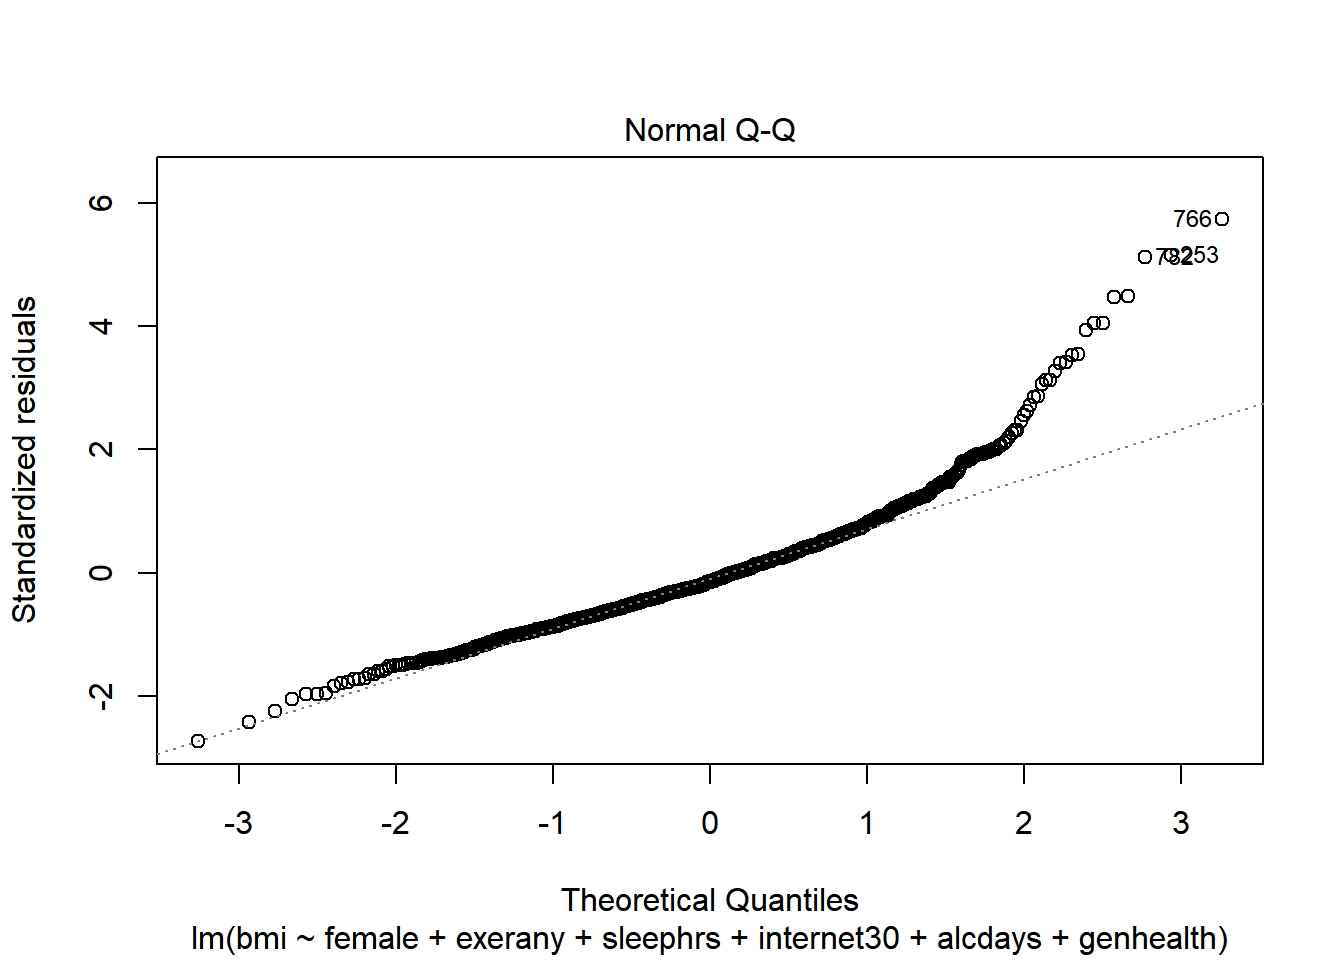
\includegraphics{bookdown-demo_files/figure-latex/c2_m6_residuals_normality-1.pdf}

\section{\texorpdfstring{\texttt{c2\_m7}: What if we added the
\texttt{menthealth}
variable?}{c2\_m7: What if we added the menthealth variable?}}\label{c2_m7-what-if-we-added-the-menthealth-variable}

\begin{Shaded}
\begin{Highlighting}[]
\NormalTok{c2_m7 <-}\StringTok{ }\KeywordTok{lm}\NormalTok{(bmi }\OperatorTok{~}\StringTok{ }\NormalTok{female }\OperatorTok{+}\StringTok{ }\NormalTok{exerany }\OperatorTok{+}\StringTok{ }\NormalTok{sleephrs }\OperatorTok{+}\StringTok{ }\NormalTok{internet30 }\OperatorTok{+}\StringTok{ }\NormalTok{alcdays }\OperatorTok{+}\StringTok{ }
\StringTok{                }\NormalTok{genhealth }\OperatorTok{+}\StringTok{ }\NormalTok{physhealth }\OperatorTok{+}\StringTok{ }\NormalTok{menthealth,}
         \DataTypeTok{data =}\NormalTok{ smartcle2)}

\KeywordTok{summary}\NormalTok{(c2_m7)}
\end{Highlighting}
\end{Shaded}

\begin{verbatim}

Call:
lm(formula = bmi ~ female + exerany + sleephrs + internet30 + 
    alcdays + genhealth + physhealth + menthealth, data = smartcle2)

Residuals:
    Min      1Q  Median      3Q     Max 
-16.060  -3.804  -0.890   2.794  33.972 

Coefficients:
                    Estimate Std. Error t value Pr(>|t|)    
(Intercept)         25.88208    1.31854  19.629  < 2e-16 ***
female              -0.96435    0.41908  -2.301 0.021616 *  
exerany             -1.43171    0.50635  -2.828 0.004797 ** 
sleephrs            -0.08033    0.13624  -0.590 0.555583    
internet30           2.00267    0.53759   3.725 0.000207 ***
alcdays             -0.07997    0.02528  -3.163 0.001614 ** 
genhealth2_VeryGood  2.09533    0.59238   3.537 0.000425 ***
genhealth3_Good      3.90949    0.60788   6.431 2.07e-10 ***
genhealth4_Fair      4.27152    0.83986   5.086 4.47e-07 ***
genhealth5_Poor      1.26021    1.31556   0.958 0.338361    
physhealth           0.06088    0.03005   2.026 0.043064 *  
menthealth           0.06636    0.03177   2.089 0.037021 *  
---
Signif. codes:  0 '***' 0.001 '**' 0.01 '*' 0.05 '.' 0.1 ' ' 1

Residual standard error: 5.964 on 884 degrees of freedom
Multiple R-squared:  0.1219,    Adjusted R-squared:  0.111 
F-statistic: 11.16 on 11 and 884 DF,  p-value: < 2.2e-16
\end{verbatim}

\section{Key Regression Assumptions for Building Effective Prediction
Models}\label{key-regression-assumptions-for-building-effective-prediction-models}

\begin{enumerate}
\def\labelenumi{\arabic{enumi}.}
\tightlist
\item
  Validity - the data you are analyzing should map to the research
  question you are trying to answer.

  \begin{itemize}
  \tightlist
  \item
    The outcome should accurately reflect the phenomenon of interest.
  \item
    The model should include all relevant predictors. (It can be
    difficult to decide which predictors are necessary, and what to do
    with predictors that have large standard errors.)
  \item
    The model should generalize to all of the cases to which it will be
    applied.
  \item
    Can the available data answer our question reliably?
  \end{itemize}
\item
  Additivity and linearity - most important assumption of a regression
  model is that its deterministic component is a linear function of the
  predictors. We often think about transformations in this setting.
\item
  Independence of errors - errors from the prediction line are
  independent of each other
\item
  Equal variance of errors - if this is violated, we can more
  efficiently estimate paramaters using \emph{weighted least squares}
  approaches, where each point is weighted inversely proportional to its
  variance, but this doesn't affect the coefficients much, if at all.
\item
  Normality of errors - not generally important for estimating the
  regression line
\end{enumerate}

\subsection{\texorpdfstring{Checking Assumptions in model
\texttt{c2\_m7}}{Checking Assumptions in model c2\_m7}}\label{checking-assumptions-in-model-c2_m7}

\begin{enumerate}
\def\labelenumi{\arabic{enumi}.}
\tightlist
\item
  How does the assumption of linearity behind this model look?
\end{enumerate}

\begin{Shaded}
\begin{Highlighting}[]
\KeywordTok{plot}\NormalTok{(c2_m7, }\DataTypeTok{which =} \DecValTok{1}\NormalTok{)}
\end{Highlighting}
\end{Shaded}

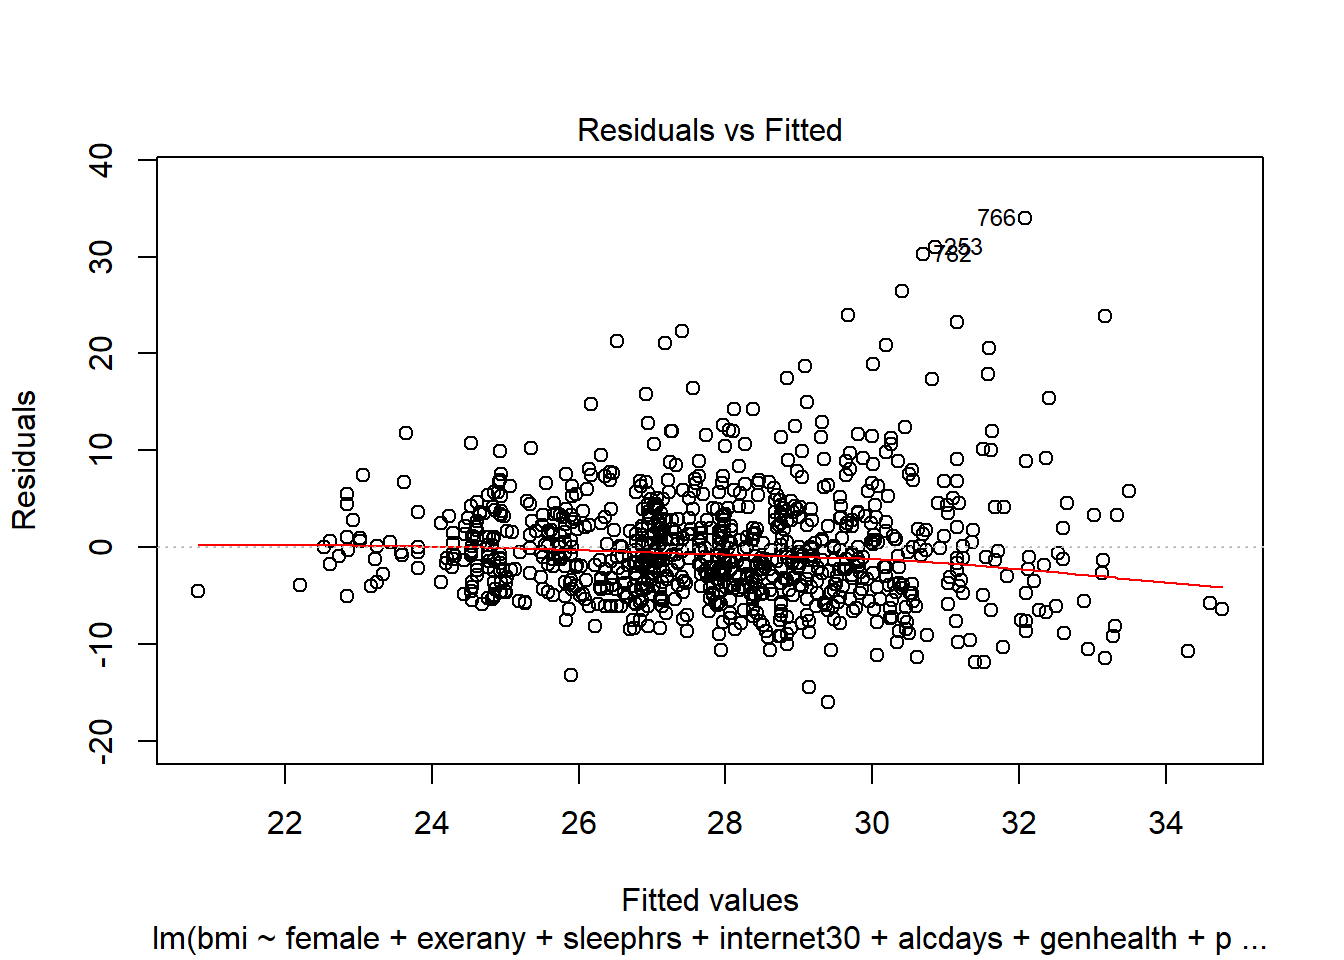
\includegraphics{bookdown-demo_files/figure-latex/residual_plot1_c2_m7-1.pdf}

We see no strong signs of serious non-linearity here. There's no obvious
curve in the plot, for example.

\begin{enumerate}
\def\labelenumi{\arabic{enumi}.}
\setcounter{enumi}{1}
\tightlist
\item
  What can we conclude from the plot below?
\end{enumerate}

\begin{Shaded}
\begin{Highlighting}[]
\KeywordTok{plot}\NormalTok{(c2_m7, }\DataTypeTok{which =} \DecValTok{5}\NormalTok{)}
\end{Highlighting}
\end{Shaded}

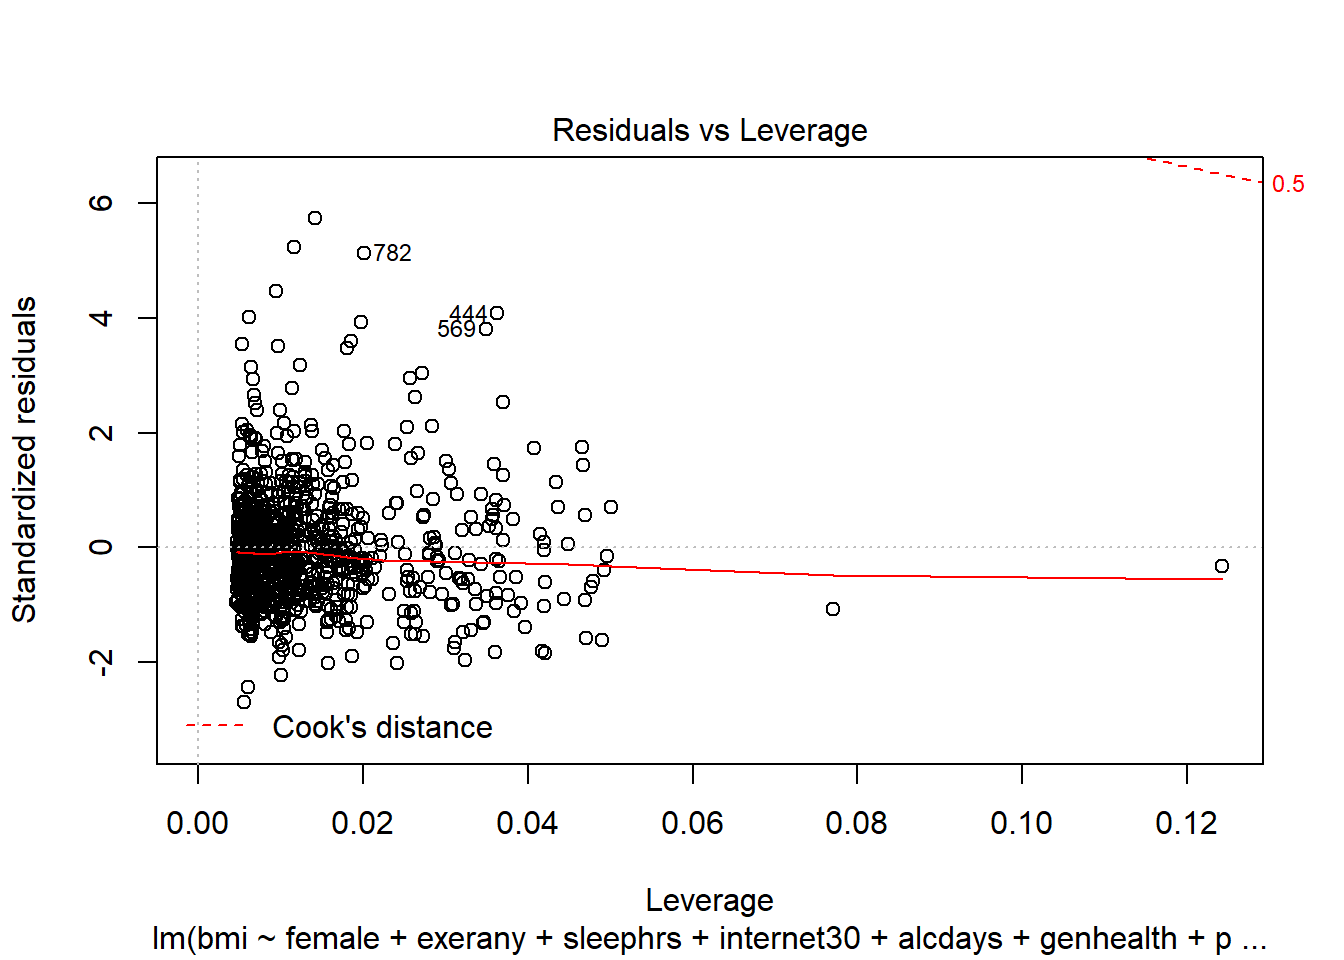
\includegraphics{bookdown-demo_files/figure-latex/residual_plot5_c2_m7-1.pdf}

This plot can help us identify points with large standardized residuals,
large leverage values, and large influence on the model (as indicated by
large values of Cook's distance.) In this case, I see no signs of any
points used in the model with especially large influence, although there
are some poorly fitted points (with especially large standardized
residuals.)

\chapter{Analysis of Variance}\label{analysis-of-variance}

\section{\texorpdfstring{The \texttt{bonding} data: A Designed Dental
Experiment}{The bonding data: A Designed Dental Experiment}}\label{the-bonding-data-a-designed-dental-experiment}

The \texttt{bonding} data describe a designed experiment into the
properties of four different resin types (\texttt{resin} = A, B, C, D)
and two different curing light sources (\texttt{light} = Halogen, LED)
as they relate to the resulting bonding strength (measured in
MPa\footnote{The MPa is defined as the failure load (in Newtons) divided
  by the entire bonded area, in mm\textsuperscript{2}.}) on the surface
of teeth. The source is \citet{Kim2014}.

The experiment involved making measurements of bonding strength under a
total of 80 experimental setups, or runs, with 10 runs completed at each
of the eight combinations of a light source and a resin type. The data
are gathered in the \texttt{bonding.csv} file.

\begin{Shaded}
\begin{Highlighting}[]
\NormalTok{bonding}
\end{Highlighting}
\end{Shaded}

\begin{verbatim}
# A tibble: 80 x 4
   run_ID light   resin strength
   <fct>  <fct>   <fct>    <dbl>
 1 R101   LED     B         12.8
 2 R102   Halogen B         22.2
 3 R103   Halogen B         24.6
 4 R104   LED     A         17.0
 5 R105   LED     C         32.2
 6 R106   Halogen B         27.1
 7 R107   LED     A         23.4
 8 R108   Halogen A         23.5
 9 R109   Halogen D         37.3
10 R110   Halogen A         19.7
# ... with 70 more rows
\end{verbatim}

\section{A One-Factor Analysis of
Variance}\label{a-one-factor-analysis-of-variance}

Suppose we are interested in the distribution of the \texttt{strength}
values for the four different types of \texttt{resin}.

\begin{Shaded}
\begin{Highlighting}[]
\NormalTok{bonding }\OperatorTok\StringTok{ }\KeywordTok{group_by}\NormalTok{(resin) }\OperatorTok\StringTok{ }\KeywordTok{summarize}\NormalTok{(}\DataTypeTok{n =} \KeywordTok{n}\NormalTok{(), }\KeywordTok{mean}\NormalTok{(strength), }\KeywordTok{median}\NormalTok{(strength))}
\end{Highlighting}
\end{Shaded}

\begin{verbatim}
# A tibble: 4 x 4
  resin     n `mean(strength)` `median(strength)`
  <fct> <int>            <dbl>              <dbl>
1 A        20             18.4               18.0
2 B        20             22.2               22.7
3 C        20             25.2               25.7
4 D        20             32.1               35.3
\end{verbatim}

I'd begin serious work with a plot.

\subsection{Look at the Data!}\label{look-at-the-data}

\begin{Shaded}
\begin{Highlighting}[]
\KeywordTok{ggplot}\NormalTok{(bonding, }\KeywordTok{aes}\NormalTok{(}\DataTypeTok{x =}\NormalTok{ resin, }\DataTypeTok{y =}\NormalTok{ strength)) }\OperatorTok{+}
\StringTok{    }\KeywordTok{geom_boxplot}\NormalTok{()}
\end{Highlighting}
\end{Shaded}

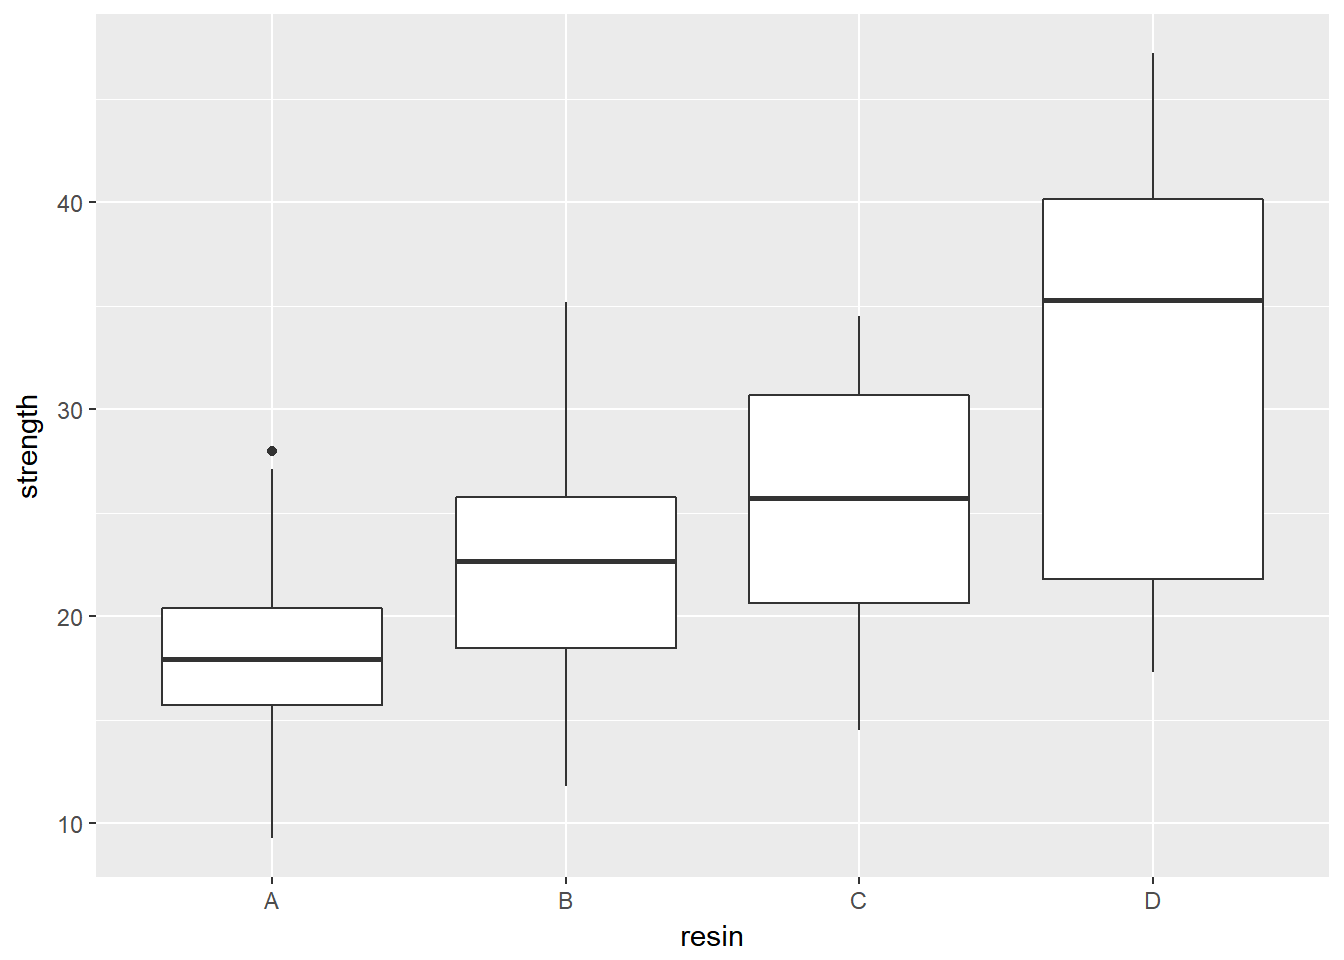
\includegraphics{bookdown-demo_files/figure-latex/c3_oneway_bonding_resin_boxplot-1.pdf}

Another good plot for this purpose is a ridgeline plot.

\begin{Shaded}
\begin{Highlighting}[]
\KeywordTok{ggplot}\NormalTok{(bonding, }\KeywordTok{aes}\NormalTok{(}\DataTypeTok{x =}\NormalTok{ strength, }\DataTypeTok{y =}\NormalTok{ resin, }\DataTypeTok{fill =}\NormalTok{ resin)) }\OperatorTok{+}
\StringTok{    }\KeywordTok{geom_density_ridges2}\NormalTok{() }\OperatorTok{+}
\StringTok{    }\KeywordTok{guides}\NormalTok{(}\DataTypeTok{fill =} \OtherTok{FALSE}\NormalTok{)}
\end{Highlighting}
\end{Shaded}

\begin{verbatim}
Picking joint bandwidth of 3.09
\end{verbatim}

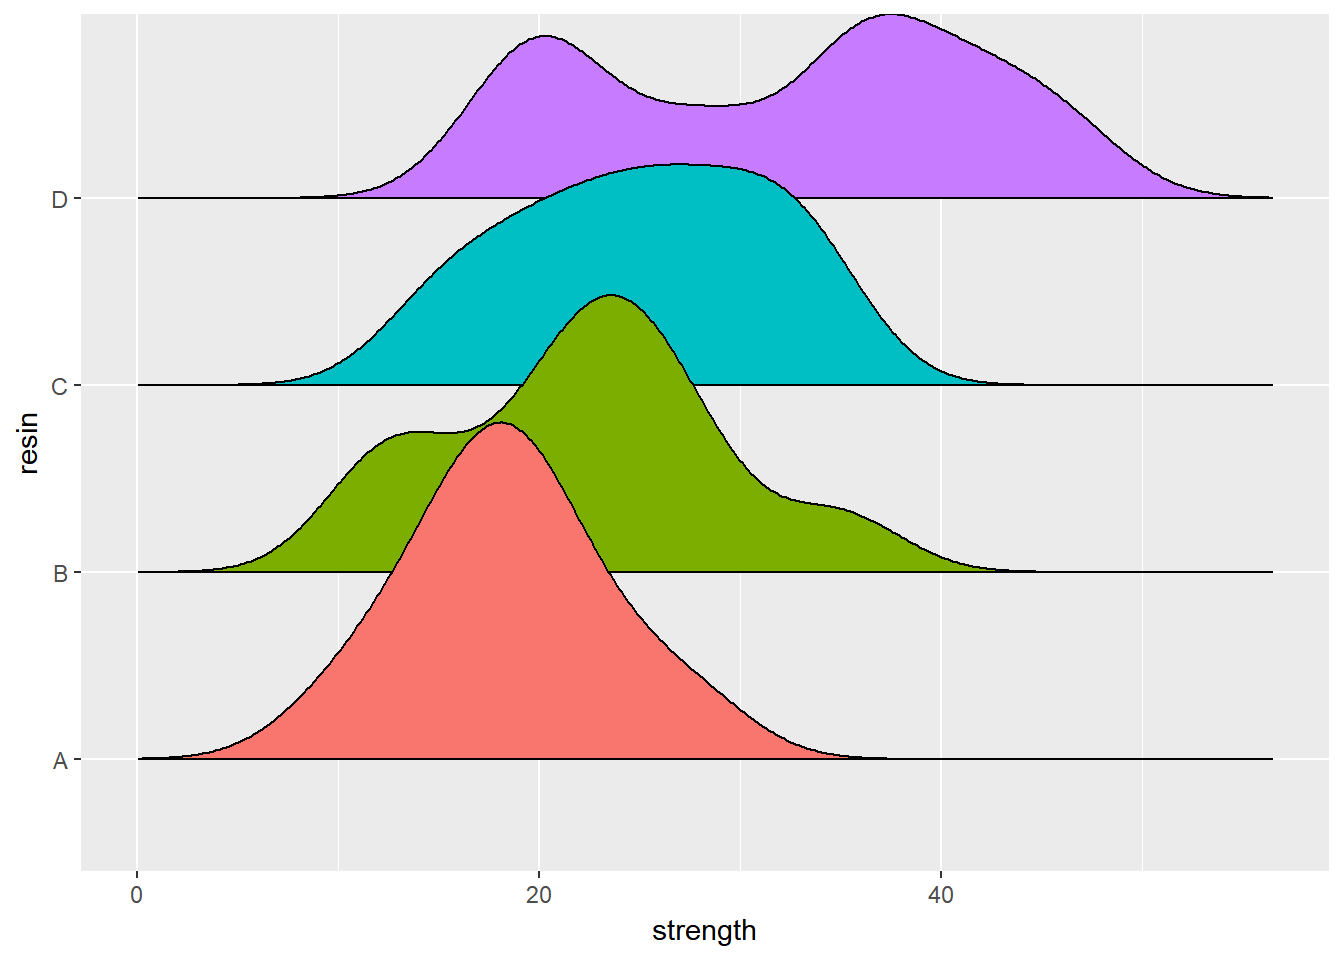
\includegraphics{bookdown-demo_files/figure-latex/c3_oneway_bonding_resin_ridgelineplot-1.pdf}

\subsection{Table of Summary
Statistics}\label{table-of-summary-statistics}

With the small size of this experiment (\emph{n} = 20 for each
\texttt{resin} type), graphical summaries may not perform as well as
they often do. We'll also produce a quick table of summary statistics
for \texttt{strength} within each \texttt{resin} type, with the
\texttt{skim()} function.

\begin{Shaded}
\begin{Highlighting}[]
\NormalTok{bonding }\OperatorTok\StringTok{ }\KeywordTok{group_by}\NormalTok{(resin) }\OperatorTok\StringTok{ }\KeywordTok{skim}\NormalTok{(strength)}
\end{Highlighting}
\end{Shaded}

\begin{verbatim}
Skim summary statistics
 n obs: 80 
 n variables: 4 
 group variables: resin 

Variable type: numeric 
 resin variable missing complete  n  mean   sd   p0   p25 median   p75
     A strength       0       20 20 18.41 4.81  9.3 15.73  17.95 20.4 
     B strength       0       20 20 22.23 6.75 11.8 18.45  22.7  25.75
     C strength       0       20 20 25.16 6.33 14.5 20.65  25.7  30.7 
     D strength       0       20 20 32.08 9.74 17.3 21.82  35.3  40.15
 p100
 28  
 35.2
 34.5
 47.2
\end{verbatim}

Since the means and medians within each group are fairly close, and the
distributions (with the possible exception of \texttt{resin} D) are
reasonably well approximated by the Normal, I'll fit an ANOVA
model\footnote{If the data weren't approximately Normally distributed,
  we might instead consider a rank-based alternative to ANOVA, like the
  Kruskal-Wallis test.}.

\begin{Shaded}
\begin{Highlighting}[]
\KeywordTok{anova}\NormalTok{(}\KeywordTok{lm}\NormalTok{(strength }\OperatorTok{~}\StringTok{ }\NormalTok{resin, }\DataTypeTok{data =}\NormalTok{ bonding))}
\end{Highlighting}
\end{Shaded}

\begin{verbatim}
Analysis of Variance Table

Response: strength
          Df Sum Sq Mean Sq F value   Pr(>F)    
resin      3 1999.7  666.57  13.107 5.52e-07 ***
Residuals 76 3865.2   50.86                     
---
Signif. codes:  0 '***' 0.001 '**' 0.01 '*' 0.05 '.' 0.1 ' ' 1
\end{verbatim}

It appears that the \texttt{resin} types have a significant association
with mean \texttt{strength} of the bonds. Can we identify which
\texttt{resin} types have generally higher or lower \texttt{strength}?

\begin{Shaded}
\begin{Highlighting}[]
\KeywordTok{TukeyHSD}\NormalTok{(}\KeywordTok{aov}\NormalTok{(}\KeywordTok{lm}\NormalTok{(strength }\OperatorTok{~}\StringTok{ }\NormalTok{resin, }\DataTypeTok{data =}\NormalTok{ bonding)))}
\end{Highlighting}
\end{Shaded}

\begin{verbatim}
  Tukey multiple comparisons of means
    95% family-wise confidence level

Fit: aov(formula = lm(strength ~ resin, data = bonding))

$resin
      diff        lwr       upr     p adj
B-A  3.815 -2.1088676  9.738868 0.3351635
C-A  6.740  0.8161324 12.663868 0.0193344
D-A 13.660  7.7361324 19.583868 0.0000003
C-B  2.925 -2.9988676  8.848868 0.5676635
D-B  9.845  3.9211324 15.768868 0.0002276
D-C  6.920  0.9961324 12.843868 0.0154615
\end{verbatim}

Based on these confidence intervals (which have a family-wise 95\%
confidence level), we see that D is associated with significantly larger
mean \texttt{strength} than A or B or C, and that C is also associated
with significantly larger mean \texttt{strength} than A. This may be
easier to see in a plot of these confidence intervals.

\begin{Shaded}
\begin{Highlighting}[]
\KeywordTok{plot}\NormalTok{(}\KeywordTok{TukeyHSD}\NormalTok{(}\KeywordTok{aov}\NormalTok{(}\KeywordTok{lm}\NormalTok{(strength }\OperatorTok{~}\StringTok{ }\NormalTok{resin, }\DataTypeTok{data =}\NormalTok{ bonding))))}
\end{Highlighting}
\end{Shaded}

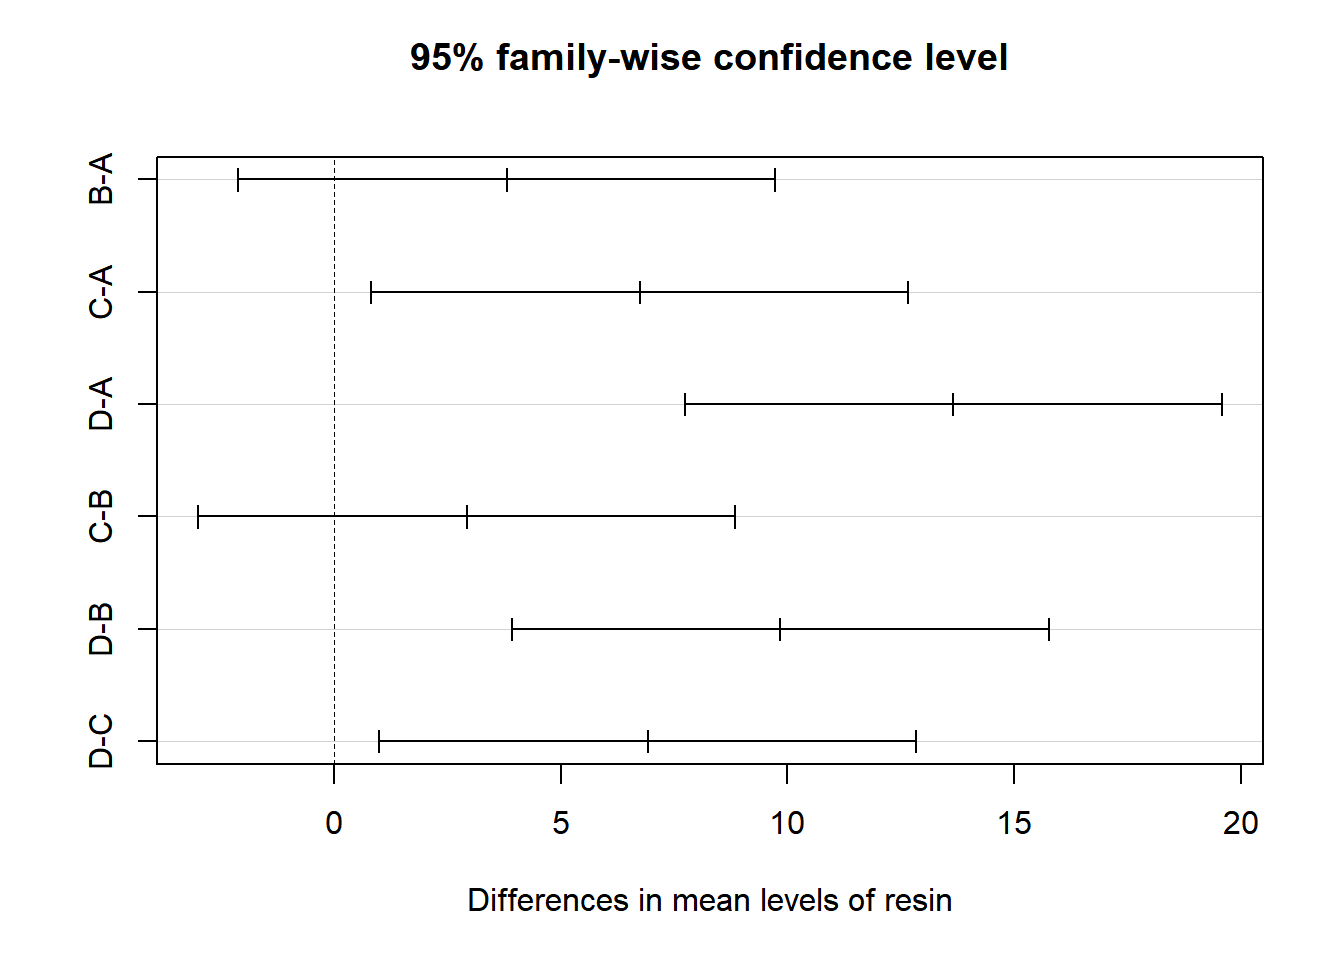
\includegraphics{bookdown-demo_files/figure-latex/unnamed-chunk-19-1.pdf}

\section{A Two-Way ANOVA: Looking at Two
Factors}\label{a-two-way-anova-looking-at-two-factors}

Now, we'll now add consideration of the \texttt{light} source into our
study. We can look at the distribution of the \texttt{strength} values
at the combinations of both \texttt{light} and \texttt{resin}, with a
plot like this one\ldots{}

\begin{Shaded}
\begin{Highlighting}[]
\KeywordTok{ggplot}\NormalTok{(bonding, }\KeywordTok{aes}\NormalTok{(}\DataTypeTok{x =}\NormalTok{ resin, }\DataTypeTok{y =}\NormalTok{ strength, }\DataTypeTok{color =}\NormalTok{ light)) }\OperatorTok{+}
\StringTok{    }\KeywordTok{geom_point}\NormalTok{(}\DataTypeTok{size =} \DecValTok{2}\NormalTok{, }\DataTypeTok{alpha =} \FloatTok{0.5}\NormalTok{) }\OperatorTok{+}
\StringTok{    }\KeywordTok{facet_wrap}\NormalTok{(}\OperatorTok{~}\StringTok{ }\NormalTok{light) }\OperatorTok{+}
\StringTok{    }\KeywordTok{guides}\NormalTok{(}\DataTypeTok{color =} \OtherTok{FALSE}\NormalTok{) }\OperatorTok{+}
\StringTok{    }\KeywordTok{scale_color_manual}\NormalTok{(}\DataTypeTok{values =} \KeywordTok{c}\NormalTok{(}\StringTok{"purple"}\NormalTok{, }\StringTok{"darkorange"}\NormalTok{)) }\OperatorTok{+}
\StringTok{    }\KeywordTok{theme_bw}\NormalTok{() }
\end{Highlighting}
\end{Shaded}

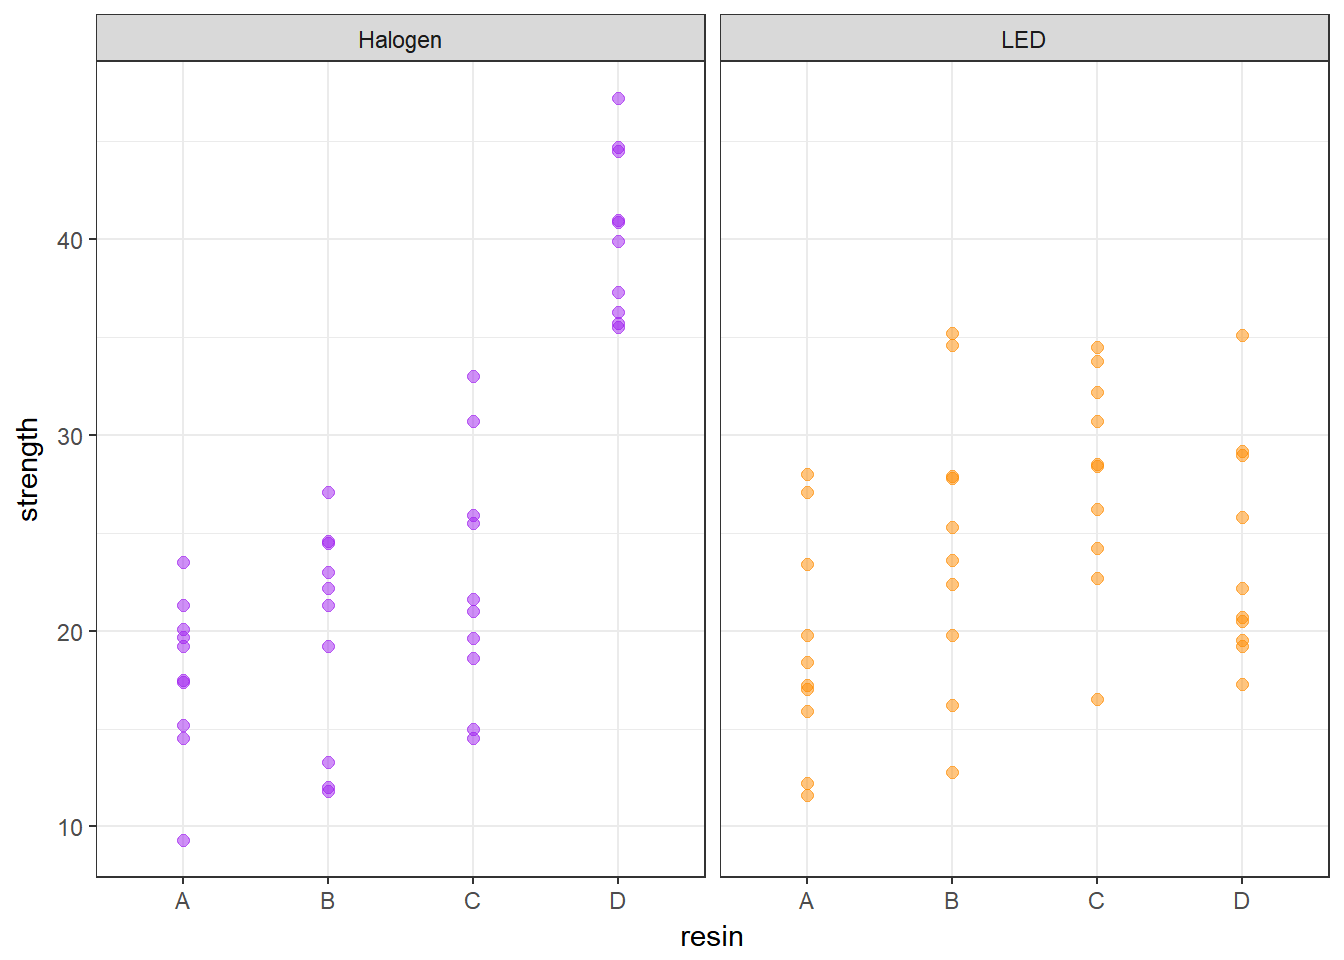
\includegraphics{bookdown-demo_files/figure-latex/c3_bonding_points_plot-1.pdf}

\section{A Means Plot (with standard deviations) to check for
interaction}\label{a-means-plot-with-standard-deviations-to-check-for-interaction}

Sometimes, we'll instead look at a plot simply of the means (and, often,
the standard deviations) of \texttt{strength} at each combination of
\texttt{light} and \texttt{resin}. We'll start by building up a data set
with the summaries we want to plot.

\begin{Shaded}
\begin{Highlighting}[]
\NormalTok{bond.sum <-}\StringTok{ }\NormalTok{bonding }\OperatorTok\StringTok{ }
\StringTok{    }\KeywordTok{group_by}\NormalTok{(resin, light) }\OperatorTok
\StringTok{    }\KeywordTok{summarize}\NormalTok{(}\DataTypeTok{mean.str =} \KeywordTok{mean}\NormalTok{(strength), }\DataTypeTok{sd.str =} \KeywordTok{sd}\NormalTok{(strength))}

\NormalTok{bond.sum}
\end{Highlighting}
\end{Shaded}

\begin{verbatim}
# A tibble: 8 x 4
# Groups:   resin [?]
  resin light   mean.str sd.str
  <fct> <fct>      <dbl>  <dbl>
1 A     Halogen     17.8   4.02
2 A     LED         19.1   5.63
3 B     Halogen     19.9   5.62
4 B     LED         24.6   7.25
5 C     Halogen     22.5   6.19
6 C     LED         27.8   5.56
7 D     Halogen     40.3   4.15
8 D     LED         23.8   5.70
\end{verbatim}

Now, we'll use this new data set to plot the means and standard
deviations of \texttt{strength} at each combination of \texttt{resin}
and \texttt{light}.

\begin{Shaded}
\begin{Highlighting}[]
\NormalTok{## The error bars will overlap unless we adjust the position.}
\NormalTok{pd <-}\StringTok{ }\KeywordTok{position_dodge}\NormalTok{(}\FloatTok{0.2}\NormalTok{) }\CommentTok{# move them .1 to the left and right}

\KeywordTok{ggplot}\NormalTok{(bond.sum, }\KeywordTok{aes}\NormalTok{(}\DataTypeTok{x =}\NormalTok{ resin, }\DataTypeTok{y =}\NormalTok{ mean.str, }\DataTypeTok{col =}\NormalTok{ light)) }\OperatorTok{+}
\StringTok{    }\KeywordTok{geom_errorbar}\NormalTok{(}\KeywordTok{aes}\NormalTok{(}\DataTypeTok{ymin =}\NormalTok{ mean.str }\OperatorTok{-}\StringTok{ }\NormalTok{sd.str, }
                      \DataTypeTok{ymax =}\NormalTok{ mean.str }\OperatorTok{+}\StringTok{ }\NormalTok{sd.str),}
                  \DataTypeTok{width =} \FloatTok{0.2}\NormalTok{, }\DataTypeTok{position =}\NormalTok{ pd) }\OperatorTok{+}
\StringTok{    }\KeywordTok{geom_point}\NormalTok{(}\DataTypeTok{size =} \DecValTok{2}\NormalTok{, }\DataTypeTok{position =}\NormalTok{ pd) }\OperatorTok{+}\StringTok{ }
\StringTok{    }\KeywordTok{geom_line}\NormalTok{(}\KeywordTok{aes}\NormalTok{(}\DataTypeTok{group =}\NormalTok{ light), }\DataTypeTok{position =}\NormalTok{ pd) }\OperatorTok{+}
\StringTok{    }\KeywordTok{scale_color_manual}\NormalTok{(}\DataTypeTok{values =} \KeywordTok{c}\NormalTok{(}\StringTok{"purple"}\NormalTok{, }\StringTok{"darkorange"}\NormalTok{)) }\OperatorTok{+}
\StringTok{    }\KeywordTok{theme_bw}\NormalTok{() }\OperatorTok{+}
\StringTok{    }\KeywordTok{labs}\NormalTok{(}\DataTypeTok{y =} \StringTok{"Bonding Strength (MPa)"}\NormalTok{, }\DataTypeTok{x =} \StringTok{"Resin Type"}\NormalTok{,}
         \DataTypeTok{title =} \StringTok{"Observed Means (+/- SD) of Bonding Strength"}\NormalTok{)}
\end{Highlighting}
\end{Shaded}

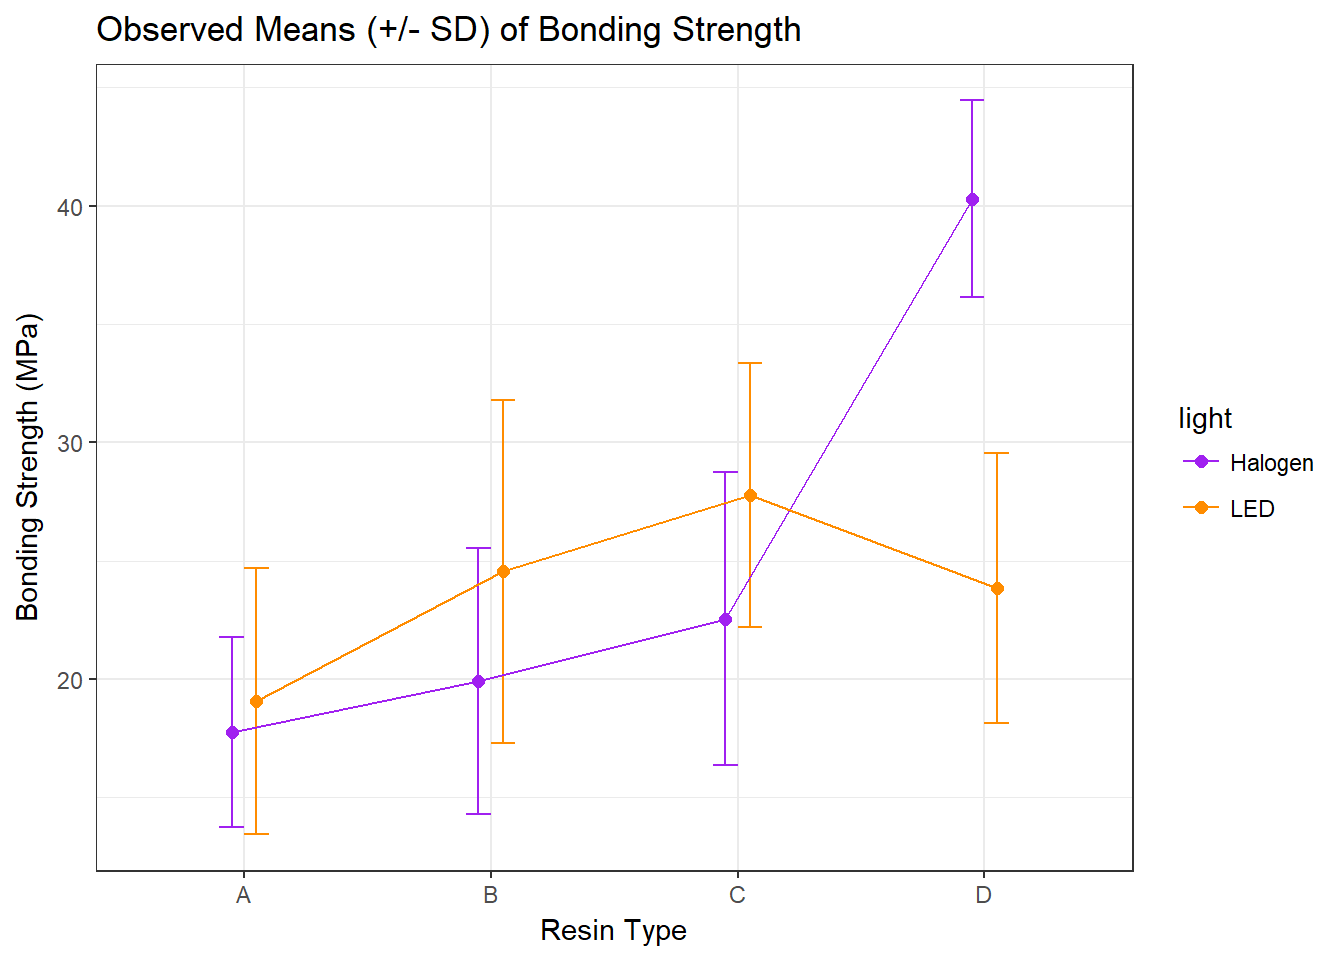
\includegraphics{bookdown-demo_files/figure-latex/c3_ggplot_means_plot_bonding-1.pdf}

Is there evidence of a meaningful interaction between the resin type and
the \texttt{light} source on the bonding strength in this plot?

\begin{itemize}
\tightlist
\item
  Sure. A meaningful interaction just means that the strength associated
  with different \texttt{resin} types depends on the \texttt{light}
  source.

  \begin{itemize}
  \tightlist
  \item
    With LED \texttt{light}, it appears that \texttt{resin} C leads to
    the strongest bonding strength.
  \item
    With Halogen \texttt{light}, though, it seems that \texttt{resin} D
    is substantially stronger.
  \end{itemize}
\item
  Note that the lines we see here connecting the \texttt{light} sources
  aren't in parallel (as they would be if we had zero interaction
  between \texttt{resin} and \texttt{light}), but rather, they cross.
\end{itemize}

\subsection{\texorpdfstring{Skimming the data after grouping by
\texttt{resin} and
\texttt{light}}{Skimming the data after grouping by resin and light}}\label{skimming-the-data-after-grouping-by-resin-and-light}

We might want to look at a numerical summary of the \texttt{strengths}
within these groups, too.

\begin{Shaded}
\begin{Highlighting}[]
\NormalTok{bonding }\OperatorTok
\StringTok{    }\KeywordTok{group_by}\NormalTok{(resin, light) }\OperatorTok
\StringTok{    }\KeywordTok{skim}\NormalTok{(strength) }
\end{Highlighting}
\end{Shaded}

\begin{verbatim}
Skim summary statistics
 n obs: 80 
 n variables: 4 
 group variables: resin, light 

Variable type: numeric 
 resin   light variable missing complete  n  mean   sd   p0   p25 median
     A Halogen strength       0       10 10 17.77 4.02  9.3 15.75  18.35
     A     LED strength       0       10 10 19.06 5.63 11.6 16.18  17.8 
     B Halogen strength       0       10 10 19.9  5.62 11.8 14.78  21.75
     B     LED strength       0       10 10 24.56 7.25 12.8 20.45  24.45
     C Halogen strength       0       10 10 22.54 6.19 14.5 18.85  21.3 
     C     LED strength       0       10 10 27.77 5.56 16.5 24.7   28.45
     D Halogen strength       0       10 10 40.3  4.15 35.5 36.55  40.4 
     D     LED strength       0       10 10 23.85 5.7  17.3 19.75  21.45
   p75 p100
 20    23.5
 22.5  28  
 24.12 27.1
 27.87 35.2
 25.8  33  
 31.83 34.5
 43.62 47.2
 28.2  35.1
\end{verbatim}

\section{Fitting the Two-Way ANOVA model with
Interaction}\label{fitting-the-two-way-anova-model-with-interaction}

\begin{Shaded}
\begin{Highlighting}[]
\NormalTok{c3_m1 <-}\StringTok{ }\KeywordTok{lm}\NormalTok{(strength }\OperatorTok{~}\StringTok{ }\NormalTok{resin }\OperatorTok{*}\StringTok{ }\NormalTok{light, }\DataTypeTok{data =}\NormalTok{ bonding)}

\KeywordTok{summary}\NormalTok{(c3_m1)}
\end{Highlighting}
\end{Shaded}

\begin{verbatim}

Call:
lm(formula = strength ~ resin * light, data = bonding)

Residuals:
    Min      1Q  Median      3Q     Max 
-11.760  -3.663  -0.320   3.697  11.250 

Coefficients:
                Estimate Std. Error t value Pr(>|t|)    
(Intercept)       17.770      1.771  10.033 2.57e-15 ***
resinB             2.130      2.505   0.850   0.3979    
resinC             4.770      2.505   1.904   0.0609 .  
resinD            22.530      2.505   8.995 2.13e-13 ***
lightLED           1.290      2.505   0.515   0.6081    
resinB:lightLED    3.370      3.542   0.951   0.3446    
resinC:lightLED    3.940      3.542   1.112   0.2697    
resinD:lightLED  -17.740      3.542  -5.008 3.78e-06 ***
---
Signif. codes:  0 '***' 0.001 '**' 0.01 '*' 0.05 '.' 0.1 ' ' 1

Residual standard error: 5.601 on 72 degrees of freedom
Multiple R-squared:  0.6149,    Adjusted R-squared:  0.5775 
F-statistic: 16.42 on 7 and 72 DF,  p-value: 9.801e-13
\end{verbatim}

\subsection{The ANOVA table for our
model}\label{the-anova-table-for-our-model}

In a two-way ANOVA model, we begin by assessing the interaction term. If
it's important, then our best model is the model including the
interaction. If it's not important, we will often move on to consider a
new model, fit without an interaction.

The ANOVA table is especially helpful in this case, because it lets us
look specifically at the interaction effect.

\begin{Shaded}
\begin{Highlighting}[]
\KeywordTok{anova}\NormalTok{(c3_m1)}
\end{Highlighting}
\end{Shaded}

\begin{verbatim}
Analysis of Variance Table

Response: strength
            Df  Sum Sq Mean Sq F value    Pr(>F)    
resin        3 1999.72  666.57 21.2499 5.792e-10 ***
light        1   34.72   34.72  1.1067    0.2963    
resin:light  3 1571.96  523.99 16.7043 2.457e-08 ***
Residuals   72 2258.52   31.37                      
---
Signif. codes:  0 '***' 0.001 '**' 0.01 '*' 0.05 '.' 0.1 ' ' 1
\end{verbatim}

\subsection{Is the interaction
important?}\label{is-the-interaction-important}

In this case, the interaction:

\begin{itemize}
\tightlist
\item
  is evident in the means plot, and
\item
  is highly statistically significant, and
\item
  accounts for a sizeable fraction (27\%) of the overall variation
\end{itemize}

\[ 
\eta^2_{interaction} = \frac{\mbox{SS(resin:light)}}{SS(Total)}
= \frac{1571.96}{1999.72 + 34.72 + 1571.96 + 2258.52} = 0.268
\]

If the interaction were \emph{either} large or significant we would be
inclined to keep it in the model. In this case, it's both, so there's no
real reason to remove it.

\subsection{Interpreting the
Interaction}\label{interpreting-the-interaction}

Recall the model equation, which is:

\begin{Shaded}
\begin{Highlighting}[]
\NormalTok{c3_m1}
\end{Highlighting}
\end{Shaded}

\begin{verbatim}

Call:
lm(formula = strength ~ resin * light, data = bonding)

Coefficients:
    (Intercept)           resinB           resinC           resinD  
          17.77             2.13             4.77            22.53  
       lightLED  resinB:lightLED  resinC:lightLED  resinD:lightLED  
           1.29             3.37             3.94           -17.74  
\end{verbatim}

so we have:

\[
strength = 17.77 + 2.13 resinB + 4.77 resinC + 22.53 resinD \\
+ 1.29 lightLED + 3.37 resinB*lightLED \\
+ 3.94 resinC*lightLED - 17.74 resinD*lightLED
\]

So, if \texttt{light} = Halogen, our equation is:

\[
strength = 17.77 + 2.13 resinB + 4.77 resinC + 22.53 resinD 
\]

And if \texttt{light} = LED, our equation is:

\[
strength = 19.06 + 5.50 resinB + 8.71 resinC + 4.79 resinD 
\]

Note that both the intercept and the slopes change as a result of the
interaction. The model yields a different prediction for every possible
combination of a \texttt{resin} type and a \texttt{light} source.

\section{\texorpdfstring{Comparing Individual Combinations of
\texttt{resin} and
\texttt{light}}{Comparing Individual Combinations of resin and light}}\label{comparing-individual-combinations-of-resin-and-light}

To make comparisons between individual combinations of a \texttt{resin}
type and a \texttt{light} source, using something like Tukey's HSD
approach for multiple comparisons, we first refit the model using the
\texttt{aov} structure, rather than \texttt{lm}.

\begin{Shaded}
\begin{Highlighting}[]
\NormalTok{c3m1_aov <-}\StringTok{ }\KeywordTok{aov}\NormalTok{(strength }\OperatorTok{~}\StringTok{ }\NormalTok{resin }\OperatorTok{*}\StringTok{ }\NormalTok{light, }\DataTypeTok{data =}\NormalTok{ bonding)}

\KeywordTok{summary}\NormalTok{(c3m1_aov)}
\end{Highlighting}
\end{Shaded}

\begin{verbatim}
            Df Sum Sq Mean Sq F value   Pr(>F)    
resin        3 1999.7   666.6  21.250 5.79e-10 ***
light        1   34.7    34.7   1.107    0.296    
resin:light  3 1572.0   524.0  16.704 2.46e-08 ***
Residuals   72 2258.5    31.4                     
---
Signif. codes:  0 '***' 0.001 '**' 0.01 '*' 0.05 '.' 0.1 ' ' 1
\end{verbatim}

And now, we can obtain Tukey HSD comparisons (which will maintain an
overall 95\% family-wise confidence level) across the \texttt{resin}
types, the \texttt{light} sources, and the combinations, with the
TukeyHSD command. This approach is only completely appropriate if these
comparisons are pre-planned, and if the design is balanced (as this is,
with the same sample size for each combination of a \texttt{light}
source and \texttt{resin} type.)

\begin{Shaded}
\begin{Highlighting}[]
\KeywordTok{TukeyHSD}\NormalTok{(c3m1_aov)}
\end{Highlighting}
\end{Shaded}

\begin{verbatim}
  Tukey multiple comparisons of means
    95% family-wise confidence level

Fit: aov(formula = strength ~ resin * light, data = bonding)

$resin
      diff       lwr       upr     p adj
B-A  3.815 -0.843129  8.473129 0.1461960
C-A  6.740  2.081871 11.398129 0.0016436
D-A 13.660  9.001871 18.318129 0.0000000
C-B  2.925 -1.733129  7.583129 0.3568373
D-B  9.845  5.186871 14.503129 0.0000026
D-C  6.920  2.261871 11.578129 0.0011731

$light
               diff       lwr      upr     p adj
LED-Halogen -1.3175 -3.814042 1.179042 0.2963128

$`resin:light`
                      diff          lwr        upr     p adj
B:Halogen-A:Halogen   2.13  -5.68928258   9.949283 0.9893515
C:Halogen-A:Halogen   4.77  -3.04928258  12.589283 0.5525230
D:Halogen-A:Halogen  22.53  14.71071742  30.349283 0.0000000
A:LED-A:Halogen       1.29  -6.52928258   9.109283 0.9995485
B:LED-A:Halogen       6.79  -1.02928258  14.609283 0.1361092
C:LED-A:Halogen      10.00   2.18071742  17.819283 0.0037074
D:LED-A:Halogen       6.08  -1.73928258  13.899283 0.2443200
C:Halogen-B:Halogen   2.64  -5.17928258  10.459283 0.9640100
D:Halogen-B:Halogen  20.40  12.58071742  28.219283 0.0000000
A:LED-B:Halogen      -0.84  -8.65928258   6.979283 0.9999747
B:LED-B:Halogen       4.66  -3.15928258  12.479283 0.5818695
C:LED-B:Halogen       7.87   0.05071742  15.689283 0.0473914
D:LED-B:Halogen       3.95  -3.86928258  11.769283 0.7621860
D:Halogen-C:Halogen  17.76   9.94071742  25.579283 0.0000000
A:LED-C:Halogen      -3.48 -11.29928258   4.339283 0.8591455
B:LED-C:Halogen       2.02  -5.79928258   9.839283 0.9922412
C:LED-C:Halogen       5.23  -2.58928258  13.049283 0.4323859
D:LED-C:Halogen       1.31  -6.50928258   9.129283 0.9995004
A:LED-D:Halogen     -21.24 -29.05928258 -13.420717 0.0000000
B:LED-D:Halogen     -15.74 -23.55928258  -7.920717 0.0000006
C:LED-D:Halogen     -12.53 -20.34928258  -4.710717 0.0001014
D:LED-D:Halogen     -16.45 -24.26928258  -8.630717 0.0000002
B:LED-A:LED           5.50  -2.31928258  13.319283 0.3665620
C:LED-A:LED           8.71   0.89071742  16.529283 0.0185285
D:LED-A:LED           4.79  -3.02928258  12.609283 0.5471915
C:LED-B:LED           3.21  -4.60928258  11.029283 0.9027236
D:LED-B:LED          -0.71  -8.52928258   7.109283 0.9999920
D:LED-C:LED          -3.92 -11.73928258   3.899283 0.7690762
\end{verbatim}

One conclusion from this is that the combination of D and Halogen is
significantly stronger than each of the other seven combinations.

\section{\texorpdfstring{The \texttt{bonding} model without
Interaction}{The bonding model without Interaction}}\label{the-bonding-model-without-interaction}

It seems incorrect in this situation to fit a model without the
interaction term, but we'll do so just so you can see what's involved.

\begin{Shaded}
\begin{Highlighting}[]
\NormalTok{c3_m2 <-}\StringTok{ }\KeywordTok{lm}\NormalTok{(strength }\OperatorTok{~}\StringTok{ }\NormalTok{resin }\OperatorTok{+}\StringTok{ }\NormalTok{light, }\DataTypeTok{data =}\NormalTok{ bonding)}

\KeywordTok{summary}\NormalTok{(c3_m2)}
\end{Highlighting}
\end{Shaded}

\begin{verbatim}

Call:
lm(formula = strength ~ resin + light, data = bonding)

Residuals:
     Min       1Q   Median       3Q      Max 
-14.1163  -4.9531   0.1187   4.4613  14.4663 

Coefficients:
            Estimate Std. Error t value Pr(>|t|)    
(Intercept)   19.074      1.787  10.676  < 2e-16 ***
resinB         3.815      2.260   1.688  0.09555 .  
resinC         6.740      2.260   2.982  0.00386 ** 
resinD        13.660      2.260   6.044 5.39e-08 ***
lightLED      -1.317      1.598  -0.824  0.41229    
---
Signif. codes:  0 '***' 0.001 '**' 0.01 '*' 0.05 '.' 0.1 ' ' 1

Residual standard error: 7.147 on 75 degrees of freedom
Multiple R-squared:  0.3469,    Adjusted R-squared:  0.312 
F-statistic: 9.958 on 4 and 75 DF,  p-value: 1.616e-06
\end{verbatim}

In the no-interaction model, if \texttt{light} = Halogen, our equation
is:

\[
strength = 19.07 + 3.82 resinB + 6.74 resinC + 13.66 resinD
\]

And if \texttt{light} = LED, our equation is:

\[
strength = 17.75 + 3.82 resinB + 6.74 resinC + 13.66 resinD
\]

So, in the no-interaction model, only the intercept changes.

\begin{Shaded}
\begin{Highlighting}[]
\KeywordTok{anova}\NormalTok{(c3_m2)}
\end{Highlighting}
\end{Shaded}

\begin{verbatim}
Analysis of Variance Table

Response: strength
          Df Sum Sq Mean Sq F value    Pr(>F)    
resin      3 1999.7  666.57 13.0514 6.036e-07 ***
light      1   34.7   34.72  0.6797    0.4123    
Residuals 75 3830.5   51.07                      
---
Signif. codes:  0 '***' 0.001 '**' 0.01 '*' 0.05 '.' 0.1 ' ' 1
\end{verbatim}

And, it appears, if we ignore the interaction, then \texttt{resin} type
has a significant impact on \texttt{strength} but \texttt{light} source
doesn't. This is clearer when we look at boxplots of the separated
\texttt{light} and \texttt{resin} groups.

\begin{Shaded}
\begin{Highlighting}[]
\NormalTok{p1 <-}\StringTok{ }\KeywordTok{ggplot}\NormalTok{(bonding, }\KeywordTok{aes}\NormalTok{(}\DataTypeTok{x =}\NormalTok{ light, }\DataTypeTok{y =}\NormalTok{ strength)) }\OperatorTok{+}\StringTok{ }
\StringTok{    }\KeywordTok{geom_boxplot}\NormalTok{()}
\NormalTok{p2 <-}\StringTok{ }\KeywordTok{ggplot}\NormalTok{(bonding, }\KeywordTok{aes}\NormalTok{(}\DataTypeTok{x =}\NormalTok{ resin, }\DataTypeTok{y =}\NormalTok{ strength)) }\OperatorTok{+}
\StringTok{    }\KeywordTok{geom_boxplot}\NormalTok{()}

\NormalTok{gridExtra}\OperatorTok{::}\KeywordTok{grid.arrange}\NormalTok{(p1, p2, }\DataTypeTok{nrow =} \DecValTok{1}\NormalTok{)}
\end{Highlighting}
\end{Shaded}

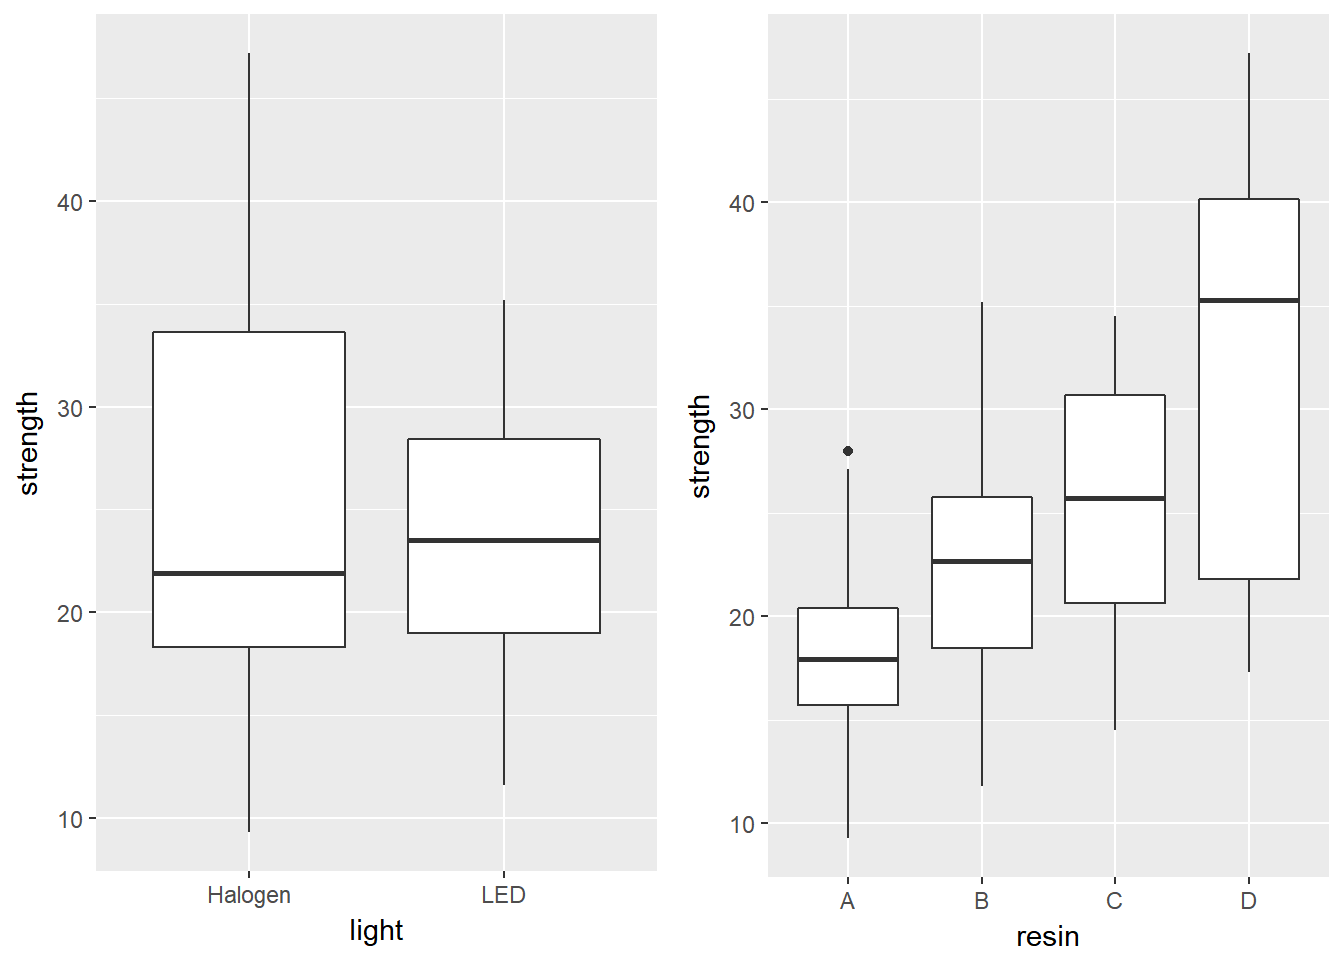
\includegraphics{bookdown-demo_files/figure-latex/boxplots_c3_bonding_without_interaction-1.pdf}

\section{\texorpdfstring{\texttt{cortisol}: A Hypothetical Clinical
Trial}{cortisol: A Hypothetical Clinical Trial}}\label{cortisol-a-hypothetical-clinical-trial}

156 adults who complained of problems with a high-stress lifestyle were
enrolled in a hypothetical clinical trial of the effectiveness of a
behavioral intervention designed to help reduce stress levels, as
measured by salivary cortisol.

The subjects were randomly assigned to one of three intervention groups
(usual care, low dose, and high dose.) The ``low dose'' subjects
received a one-week intervention with a follow-up at week 5. The ``high
dose'' subjects received a more intensive three-week intervention, with
follow up at week 5.

Since cortisol levels rise and fall with circadian rhythms, the cortisol
measurements were taken just after rising for all subjects. These
measurements were taken at baseline, and again at five weeks. The
difference (baseline - week 5) in cortisol level (in micrograms / l)
serves as the primary outcome.

\subsection{\texorpdfstring{Codebook and Raw Data for
\texttt{cortisol}}{Codebook and Raw Data for cortisol}}\label{codebook-and-raw-data-for-cortisol}

The data are gathered in the \texttt{cortisol} data set. Included are:

\begin{longtable}[]{@{}rl@{}}
\toprule
Variable & Description\tabularnewline
\midrule
\endhead
\texttt{subject} & subject identification code\tabularnewline
\texttt{interv} & intervention group (UC = usual care, Low,
High)\tabularnewline
\texttt{waist} & waist circumference at baseline (in
inches)\tabularnewline
\texttt{sex} & male or female\tabularnewline
\texttt{cort.1} & salivary cortisol level (microg/l) week
1\tabularnewline
\texttt{cort.5} & salivary cortisol level (microg/l) week
5\tabularnewline
\bottomrule
\end{longtable}

\begin{Shaded}
\begin{Highlighting}[]
\NormalTok{cortisol}
\end{Highlighting}
\end{Shaded}

\begin{verbatim}
# A tibble: 156 x 6
   subject interv waist sex   cort.1 cort.5
     <int> <fct>  <dbl> <fct>  <dbl>  <dbl>
 1    1001 UC      48.3 M      13.4   13.3 
 2    1002 Low     58.3 M      17.8   16.6 
 3    1003 High    43.0 M      14.4   12.7 
 4    1004 Low     44.9 M       9.00   9.80
 5    1005 High    46.1 M      14.2   14.2 
 6    1006 UC      41.3 M      14.8   15.1 
 7    1007 Low     51.0 F      13.7   16.0 
 8    1008 UC      42.0 F      17.3   18.7 
 9    1009 Low     24.7 F      15.3   15.8 
10    1010 Low     59.4 M      12.4   11.7 
# ... with 146 more rows
\end{verbatim}

\section{Creating a factor combining sex and
waist}\label{creating-a-factor-combining-sex-and-waist}

Next, we'll put the \texttt{waist} and \texttt{sex} data in the
\texttt{cortisol} example together. We want to build a second
categorical variable (called \texttt{fat\_est}) combining this
information, to indicate ``healthy'' vs. ``unhealthy'' levels of fat
around the waist.

\begin{itemize}
\tightlist
\item
  Male subjects whose waist circumference is 40 inches or more, and
\item
  Female subjects whose waist circumference is 35 inches or more, will
  fall in the ``unhealthy'' group.
\end{itemize}

\begin{Shaded}
\begin{Highlighting}[]
\NormalTok{cortisol <-}\StringTok{ }\NormalTok{cortisol }\OperatorTok
\StringTok{    }\KeywordTok{mutate}\NormalTok{(}
        \DataTypeTok{fat_est =} \KeywordTok{factor}\NormalTok{(}\KeywordTok{case_when}\NormalTok{(}
\NormalTok{            sex }\OperatorTok{==}\StringTok{ "M"} \OperatorTok{&}\StringTok{ }\NormalTok{waist }\OperatorTok{>=}\StringTok{ }\DecValTok{40} \OperatorTok{~}\StringTok{ "unhealthy"}\NormalTok{,}
\NormalTok{            sex }\OperatorTok{==}\StringTok{ "F"} \OperatorTok{&}\StringTok{ }\NormalTok{waist }\OperatorTok{>=}\StringTok{ }\DecValTok{35} \OperatorTok{~}\StringTok{ "unhealthy"}\NormalTok{,}
            \OtherTok{TRUE}                     \OperatorTok{~}\StringTok{ "healthy"}\NormalTok{)),}
        \DataTypeTok{cort_diff =}\NormalTok{ cort.}\DecValTok{1} \OperatorTok{-}\StringTok{ }\NormalTok{cort.}\DecValTok{5}\NormalTok{)}

\KeywordTok{summary}\NormalTok{(cortisol)}
\end{Highlighting}
\end{Shaded}

\begin{verbatim}
    subject      interv       waist       sex        cort.1      
 Min.   :1001   High:53   Min.   :20.80   F:83   Min.   : 6.000  
 1st Qu.:1040   Low :52   1st Qu.:33.27   M:73   1st Qu.: 9.675  
 Median :1078   UC  :51   Median :40.35          Median :12.400  
 Mean   :1078             Mean   :40.42          Mean   :12.686  
 3rd Qu.:1117             3rd Qu.:47.77          3rd Qu.:16.025  
 Max.   :1156             Max.   :59.90          Max.   :19.000  
     cort.5          fat_est      cort_diff      
 Min.   : 4.2   healthy  : 56   Min.   :-2.3000  
 1st Qu.: 9.6   unhealthy:100   1st Qu.:-0.5000  
 Median :12.6                   Median : 0.2000  
 Mean   :12.4                   Mean   : 0.2821  
 3rd Qu.:15.7                   3rd Qu.: 1.2000  
 Max.   :19.7                   Max.   : 2.0000  
\end{verbatim}

\section{\texorpdfstring{A Means Plot for the \texttt{cortisol} trial
(with standard
errors)}{A Means Plot for the cortisol trial (with standard errors)}}\label{a-means-plot-for-the-cortisol-trial-with-standard-errors}

Again, we'll start by building up a data set with the summaries we want
to plot.

\begin{Shaded}
\begin{Highlighting}[]
\NormalTok{cort.sum <-}\StringTok{ }\NormalTok{cortisol }\OperatorTok\StringTok{ }
\StringTok{    }\KeywordTok{group_by}\NormalTok{(interv, fat_est) }\OperatorTok
\StringTok{    }\KeywordTok{summarize}\NormalTok{(}\DataTypeTok{mean.cort =} \KeywordTok{mean}\NormalTok{(cort_diff), }
              \DataTypeTok{se.cort =} \KeywordTok{sd}\NormalTok{(cort_diff)}\OperatorTok{/}\KeywordTok{sqrt}\NormalTok{(}\KeywordTok{n}\NormalTok{()))}

\NormalTok{cort.sum}
\end{Highlighting}
\end{Shaded}

\begin{verbatim}
# A tibble: 6 x 4
# Groups:   interv [?]
  interv fat_est   mean.cort se.cort
  <fct>  <fct>         <dbl>   <dbl>
1 High   healthy       0.695   0.217
2 High   unhealthy     0.352   0.150
3 Low    healthy       0.500   0.182
4 Low    unhealthy     0.327   0.190
5 UC     healthy       0.347   0.225
6 UC     unhealthy    -0.226   0.155
\end{verbatim}

Now, we'll use this new data set to plot the means and standard errors.

\begin{Shaded}
\begin{Highlighting}[]
\NormalTok{## The error bars will overlap unless we adjust the position.}
\NormalTok{pd <-}\StringTok{ }\KeywordTok{position_dodge}\NormalTok{(}\FloatTok{0.2}\NormalTok{) }\CommentTok{# move them .1 to the left and right}

\KeywordTok{ggplot}\NormalTok{(cort.sum, }\KeywordTok{aes}\NormalTok{(}\DataTypeTok{x =}\NormalTok{ interv, }\DataTypeTok{y =}\NormalTok{ mean.cort, }\DataTypeTok{col =}\NormalTok{ fat_est)) }\OperatorTok{+}
\StringTok{    }\KeywordTok{geom_errorbar}\NormalTok{(}\KeywordTok{aes}\NormalTok{(}\DataTypeTok{ymin =}\NormalTok{ mean.cort }\OperatorTok{-}\StringTok{ }\NormalTok{se.cort, }
                      \DataTypeTok{ymax =}\NormalTok{ mean.cort }\OperatorTok{+}\StringTok{ }\NormalTok{se.cort),}
                  \DataTypeTok{width =} \FloatTok{0.2}\NormalTok{, }\DataTypeTok{position =}\NormalTok{ pd) }\OperatorTok{+}
\StringTok{    }\KeywordTok{geom_point}\NormalTok{(}\DataTypeTok{size =} \DecValTok{2}\NormalTok{, }\DataTypeTok{position =}\NormalTok{ pd) }\OperatorTok{+}\StringTok{ }
\StringTok{    }\KeywordTok{geom_line}\NormalTok{(}\KeywordTok{aes}\NormalTok{(}\DataTypeTok{group =}\NormalTok{ fat_est), }\DataTypeTok{position =}\NormalTok{ pd) }\OperatorTok{+}
\StringTok{    }\KeywordTok{scale_color_manual}\NormalTok{(}\DataTypeTok{values =} \KeywordTok{c}\NormalTok{(}\StringTok{"royalblue"}\NormalTok{, }\StringTok{"darkred"}\NormalTok{)) }\OperatorTok{+}
\StringTok{    }\KeywordTok{theme_bw}\NormalTok{() }\OperatorTok{+}
\StringTok{    }\KeywordTok{labs}\NormalTok{(}\DataTypeTok{y =} \StringTok{"Salivary Cortisol Level"}\NormalTok{, }\DataTypeTok{x =} \StringTok{"Intervention Group"}\NormalTok{,}
         \DataTypeTok{title =} \StringTok{"Observed Means (+/- SE) of Salivary Cortisol"}\NormalTok{)}
\end{Highlighting}
\end{Shaded}

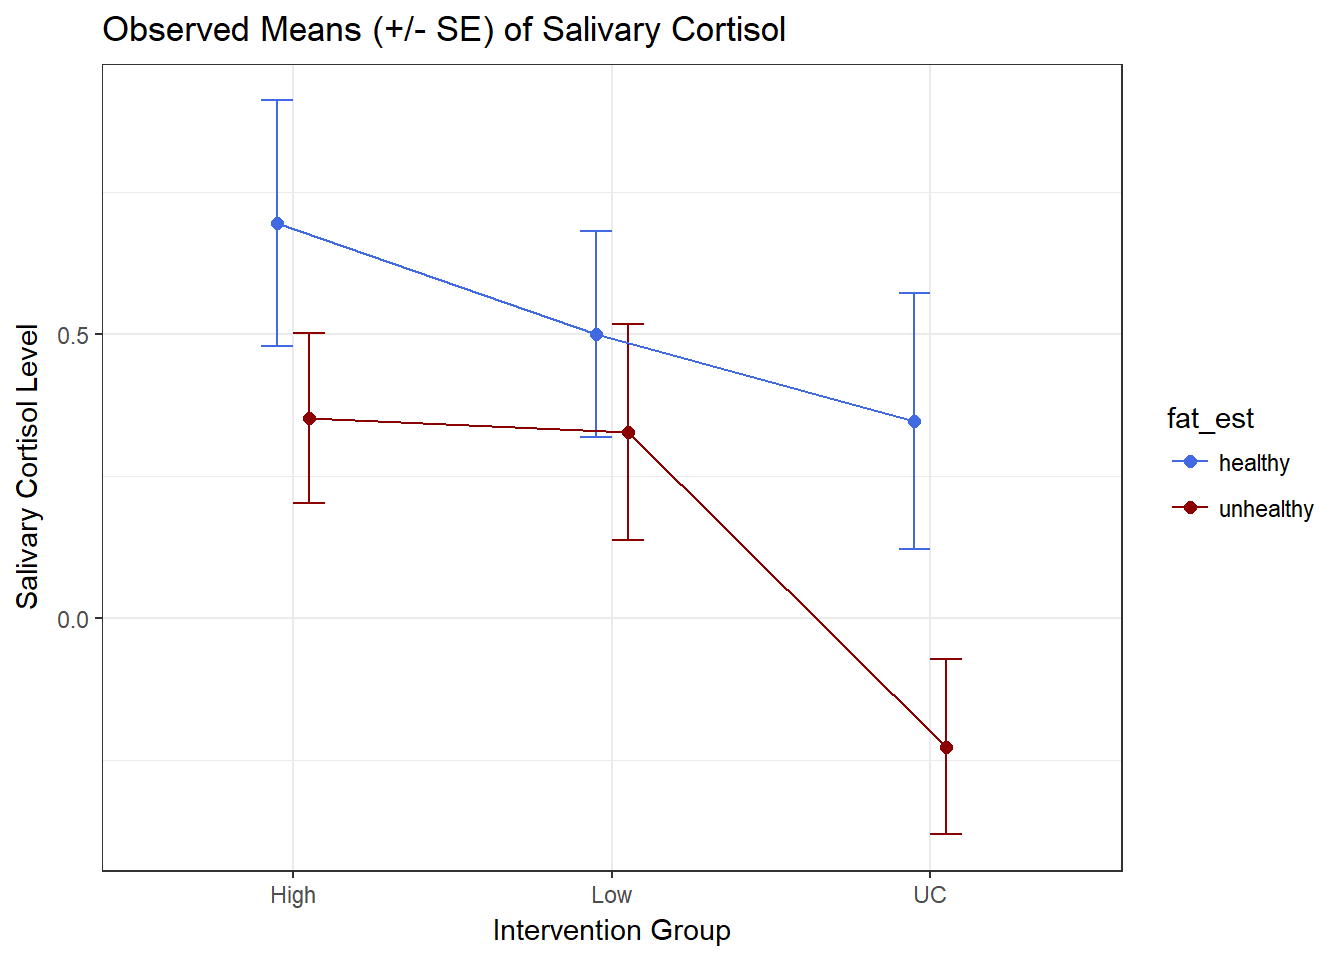
\includegraphics{bookdown-demo_files/figure-latex/c3_ggplot_means_plot_cortisol-1.pdf}

\section{\texorpdfstring{A Two-Way ANOVA model for \texttt{cortisol}
with
Interaction}{A Two-Way ANOVA model for cortisol with Interaction}}\label{a-two-way-anova-model-for-cortisol-with-interaction}

\begin{Shaded}
\begin{Highlighting}[]
\NormalTok{c3_m3 <-}\StringTok{ }\KeywordTok{lm}\NormalTok{(cort_diff }\OperatorTok{~}\StringTok{ }\NormalTok{interv }\OperatorTok{*}\StringTok{ }\NormalTok{fat_est, }\DataTypeTok{data =}\NormalTok{ cortisol)}

\KeywordTok{anova}\NormalTok{(c3_m3)}
\end{Highlighting}
\end{Shaded}

\begin{verbatim}
Analysis of Variance Table

Response: cort_diff
                Df  Sum Sq Mean Sq F value  Pr(>F)  
interv           2   7.847  3.9235  4.4698 0.01301 *
fat_est          1   4.614  4.6139  5.2564 0.02326 *
interv:fat_est   2   0.943  0.4715  0.5371 0.58554  
Residuals      150 131.666  0.8778                  
---
Signif. codes:  0 '***' 0.001 '**' 0.01 '*' 0.05 '.' 0.1 ' ' 1
\end{verbatim}

Does it seem like we need the interaction term in this case?

\begin{Shaded}
\begin{Highlighting}[]
\KeywordTok{summary}\NormalTok{(c3_m3)}
\end{Highlighting}
\end{Shaded}

\begin{verbatim}

Call:
lm(formula = cort_diff ~ interv * fat_est, data = cortisol)

Residuals:
     Min       1Q   Median       3Q      Max 
-2.62727 -0.75702  0.08636  0.84848  2.12647 

Coefficients:
                           Estimate Std. Error t value Pr(>|t|)   
(Intercept)                  0.6950     0.2095   3.317  0.00114 **
intervLow                   -0.1950     0.3001  -0.650  0.51689   
intervUC                    -0.3479     0.3091  -1.126  0.26206   
fat_estunhealthy            -0.3435     0.2655  -1.294  0.19774   
intervLow:fat_estunhealthy   0.1708     0.3785   0.451  0.65256   
intervUC:fat_estunhealthy   -0.2300     0.3846  -0.598  0.55068   
---
Signif. codes:  0 '***' 0.001 '**' 0.01 '*' 0.05 '.' 0.1 ' ' 1

Residual standard error: 0.9369 on 150 degrees of freedom
Multiple R-squared:  0.0924,    Adjusted R-squared:  0.06214 
F-statistic: 3.054 on 5 and 150 DF,  p-value: 0.01179
\end{verbatim}

How do you reconcile the apparent difference in significance levels
between this regression summary and the ANOVA table above?

\section{\texorpdfstring{A Two-Way ANOVA model for \texttt{cortisol}
without
Interaction}{A Two-Way ANOVA model for cortisol without Interaction}}\label{a-two-way-anova-model-for-cortisol-without-interaction}

\subsection{The Graph}\label{the-graph}

\begin{Shaded}
\begin{Highlighting}[]
\NormalTok{p1 <-}\StringTok{ }\KeywordTok{ggplot}\NormalTok{(cortisol, }\KeywordTok{aes}\NormalTok{(}\DataTypeTok{x =}\NormalTok{ interv, }\DataTypeTok{y =}\NormalTok{ cort_diff)) }\OperatorTok{+}\StringTok{ }
\StringTok{    }\KeywordTok{geom_boxplot}\NormalTok{()}
\NormalTok{p2 <-}\StringTok{ }\KeywordTok{ggplot}\NormalTok{(cortisol, }\KeywordTok{aes}\NormalTok{(}\DataTypeTok{x =}\NormalTok{ fat_est, }\DataTypeTok{y =}\NormalTok{ cort_diff)) }\OperatorTok{+}
\StringTok{    }\KeywordTok{geom_boxplot}\NormalTok{()}

\NormalTok{gridExtra}\OperatorTok{::}\KeywordTok{grid.arrange}\NormalTok{(p1, p2, }\DataTypeTok{nrow =} \DecValTok{1}\NormalTok{)}
\end{Highlighting}
\end{Shaded}

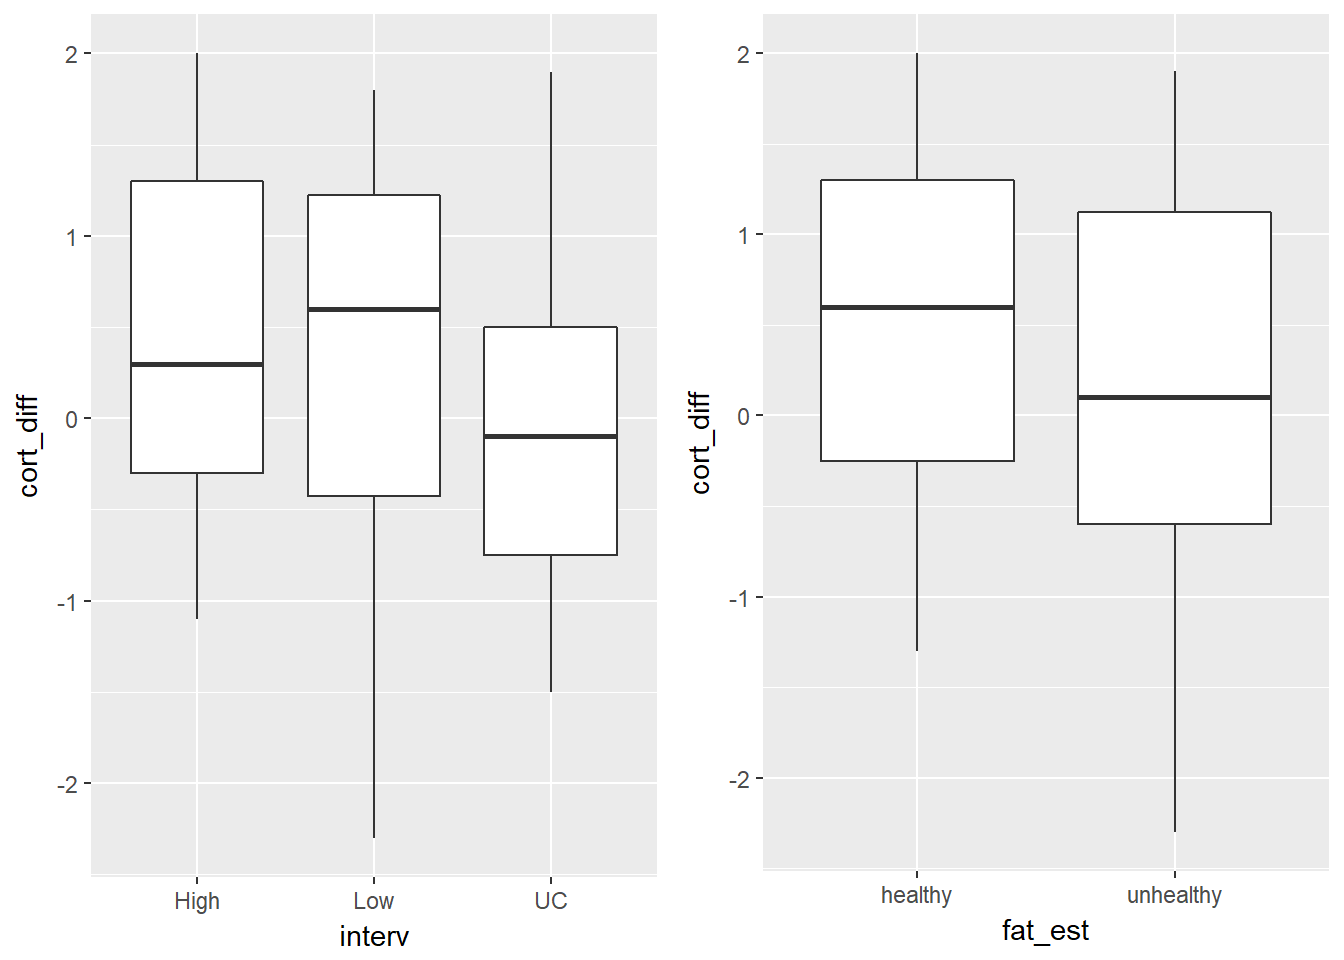
\includegraphics{bookdown-demo_files/figure-latex/boxplots_c3_cortisol_without_interaction-1.pdf}

\subsection{The ANOVA Model}\label{the-anova-model}

\begin{Shaded}
\begin{Highlighting}[]
\NormalTok{c3_m4 <-}\StringTok{ }\KeywordTok{lm}\NormalTok{(cort_diff }\OperatorTok{~}\StringTok{ }\NormalTok{interv }\OperatorTok{+}\StringTok{ }\NormalTok{fat_est, }\DataTypeTok{data =}\NormalTok{ cortisol)}

\KeywordTok{anova}\NormalTok{(c3_m4)}
\end{Highlighting}
\end{Shaded}

\begin{verbatim}
Analysis of Variance Table

Response: cort_diff
           Df  Sum Sq Mean Sq F value  Pr(>F)  
interv      2   7.847  3.9235  4.4972 0.01266 *
fat_est     1   4.614  4.6139  5.2886 0.02283 *
Residuals 152 132.609  0.8724                  
---
Signif. codes:  0 '***' 0.001 '**' 0.01 '*' 0.05 '.' 0.1 ' ' 1
\end{verbatim}

How do these results compare to those we saw in the model with
interaction?

\subsection{The Regression Summary}\label{the-regression-summary}

\begin{Shaded}
\begin{Highlighting}[]
\KeywordTok{summary}\NormalTok{(c3_m4)}
\end{Highlighting}
\end{Shaded}

\begin{verbatim}

Call:
lm(formula = cort_diff ~ interv + fat_est, data = cortisol)

Residuals:
     Min       1Q   Median       3Q      Max 
-2.55929 -0.74527  0.05457  0.86456  2.05489 

Coefficients:
                 Estimate Std. Error t value Pr(>|t|)    
(Intercept)       0.70452    0.16093   4.378 2.22e-05 ***
intervLow        -0.08645    0.18232  -0.474  0.63606    
intervUC         -0.50063    0.18334  -2.731  0.00707 ** 
fat_estunhealthy -0.35878    0.15601  -2.300  0.02283 *  
---
Signif. codes:  0 '***' 0.001 '**' 0.01 '*' 0.05 '.' 0.1 ' ' 1

Residual standard error: 0.934 on 152 degrees of freedom
Multiple R-squared:  0.0859,    Adjusted R-squared:  0.06785 
F-statistic: 4.761 on 3 and 152 DF,  p-value: 0.00335
\end{verbatim}

\subsection{Tukey HSD Comparisons}\label{tukey-hsd-comparisons}

Without the interaction term, we can make direct comparisons between
levels of the intervention, and between levels of the \texttt{fat\_est}
variable. This is probably best done here in a Tukey HSD comparison.

\begin{Shaded}
\begin{Highlighting}[]
\KeywordTok{TukeyHSD}\NormalTok{(}\KeywordTok{aov}\NormalTok{(cort_diff }\OperatorTok{~}\StringTok{ }\NormalTok{interv }\OperatorTok{+}\StringTok{ }\NormalTok{fat_est, }\DataTypeTok{data =}\NormalTok{ cortisol))}
\end{Highlighting}
\end{Shaded}

\begin{verbatim}
  Tukey multiple comparisons of means
    95% family-wise confidence level

Fit: aov(formula = cort_diff ~ interv + fat_est, data = cortisol)

$interv
                diff        lwr         upr     p adj
Low-High -0.09074746 -0.5222655  0.34077063 0.8724916
UC-High  -0.51642619 -0.9500745 -0.08277793 0.0150150
UC-Low   -0.42567873 -0.8613670  0.01000948 0.0570728

$fat_est
                        diff        lwr         upr     p adj
unhealthy-healthy -0.3582443 -0.6662455 -0.05024305 0.0229266
\end{verbatim}

What conclusions can we draw, at a 5\% significance level?

\chapter{Analysis of Covariance}\label{analysis-of-covariance}

\section{An Emphysema Study}\label{an-emphysema-study}

My source for this example is \citet{Riffenburgh2006}, section 18.4.
Serum theophylline levels (in mg/dl) were measured in 16 patients with
emphysema at baseline, then 5 days later (at the end of a course of
antibiotics) and then at 10 days after baseline. Clinicians anticipate
that the antibiotic will increase the theophylline level. The data are
stored in the \texttt{emphysema.csv} data file, and note that the age
for patient 5 is not available.

\subsection{Codebook}\label{codebook}

\begin{longtable}[]{@{}rl@{}}
\toprule
Variable & Description\tabularnewline
\midrule
\endhead
\texttt{patient} & ID code\tabularnewline
\texttt{age} & patient's age in years\tabularnewline
\texttt{sex} & patient's sex (F or M)\tabularnewline
\texttt{st\_base} & patient's serum theophylline at baseline
(mg/dl)\tabularnewline
\texttt{st\_day5} & patient's serum theophylline at day 5
(mg/dl)\tabularnewline
\texttt{st\_day10} & patient's serum theophylline at day 10
(mg/dl)\tabularnewline
\bottomrule
\end{longtable}

We're going to look at the change from baseline to day 5 as our outcome
of interest, since the clinical expectation is that the antibiotic
(azithromycin) will increase theophylline levels.

\begin{Shaded}
\begin{Highlighting}[]
\NormalTok{emphysema <-}\StringTok{ }\NormalTok{emphysema }\OperatorTok\StringTok{ }
\StringTok{    }\KeywordTok{mutate}\NormalTok{(}\DataTypeTok{st_delta =}\NormalTok{ st_day5 }\OperatorTok{-}\StringTok{ }\NormalTok{st_base)}

\NormalTok{emphysema}
\end{Highlighting}
\end{Shaded}

\begin{verbatim}
# A tibble: 16 x 7
   patient   age sex   st_base st_day5 st_day10 st_delta
     <int> <int> <fct>   <dbl>   <dbl>    <dbl>    <dbl>
 1       1    61 F       14.1     2.30    10.3   -11.8  
 2       2    70 F        7.20    5.40     7.30  - 1.80 
 3       3    65 M       14.2    11.9     11.3   - 2.30 
 4       4    65 M       10.3    10.7     13.8     0.400
 5       5    NA M        9.90   10.7     11.7     0.800
 6       6    76 M        5.20    6.80     4.20    1.60 
 7       7    72 M       10.4    14.6     14.1     4.20 
 8       8    69 F       10.5     7.20     5.40  - 3.30 
 9       9    66 M        5.00    5.00     5.10    0    
10      10    62 M        8.60    8.10     7.40  - 0.500
11      11    65 F       16.6    14.9     13.0   - 1.70 
12      12    71 M       16.4    18.6     17.1     2.20 
13      13    51 F       12.2    11.0     12.3   - 1.20 
14      14    71 M        6.60    3.70     4.50  - 2.90 
15      15    64 F       15.4    15.2     13.6   - 0.200
16      16    50 M       10.2    10.8     11.2     0.600
\end{verbatim}

\section{\texorpdfstring{Does \texttt{sex} affect the mean change in
theophylline?}{Does sex affect the mean change in theophylline?}}\label{does-sex-affect-the-mean-change-in-theophylline}

\begin{Shaded}
\begin{Highlighting}[]
\NormalTok{emphysema }\OperatorTok\StringTok{ }\KeywordTok{skim}\NormalTok{(st_delta)}
\end{Highlighting}
\end{Shaded}

\begin{verbatim}
Skim summary statistics
 n obs: 16 
 n variables: 7 

Variable type: numeric 
 variable missing complete  n  mean   sd    p0   p25 median  p75 p100
 st_delta       0       16 16 -0.99 3.48 -11.8 -1.92  -0.35 0.65  4.2
\end{verbatim}

\begin{Shaded}
\begin{Highlighting}[]
\NormalTok{emphysema }\OperatorTok\StringTok{ }\KeywordTok{group_by}\NormalTok{(sex) }\OperatorTok\StringTok{ }\KeywordTok{skim}\NormalTok{(st_delta)}
\end{Highlighting}
\end{Shaded}

\begin{verbatim}
Skim summary statistics
 n obs: 16 
 n variables: 7 
 group variables: sex 

Variable type: numeric 
 sex variable missing complete  n  mean   sd    p0   p25 median   p75 p100
   F st_delta       0        6  6 -3.33 4.27 -11.8 -2.92  -1.75 -1.32 -0.2
   M st_delta       0       10 10  0.41 2.07  -2.9 -0.38   0.5   1.4   4.2
\end{verbatim}

Overall, the mean change in theophylline during the course of the
antibiotic is -0.99, but this is -3.33 for female patients and 0.41 for
male patients.

A one-way ANOVA model looks like this:

\begin{Shaded}
\begin{Highlighting}[]
\KeywordTok{anova}\NormalTok{(}\KeywordTok{lm}\NormalTok{(st_delta }\OperatorTok{~}\StringTok{ }\NormalTok{sex, }\DataTypeTok{data =}\NormalTok{ emphysema))}
\end{Highlighting}
\end{Shaded}

\begin{verbatim}
Analysis of Variance Table

Response: st_delta
          Df  Sum Sq Mean Sq F value  Pr(>F)  
sex        1  52.547  52.547  5.6789 0.03189 *
Residuals 14 129.542   9.253                  
---
Signif. codes:  0 '***' 0.001 '**' 0.01 '*' 0.05 '.' 0.1 ' ' 1
\end{verbatim}

The ANOVA F test finds a statistically significant difference between
the mean \texttt{st\_delta} among males and the mean \texttt{st\_delta}
among females. But is there more to the story?

\section{\texorpdfstring{Is there an association between \texttt{age}
and \texttt{sex} in this
study?}{Is there an association between age and sex in this study?}}\label{is-there-an-association-between-age-and-sex-in-this-study}

\begin{Shaded}
\begin{Highlighting}[]
\NormalTok{emphysema }\OperatorTok\StringTok{ }\KeywordTok{group_by}\NormalTok{(sex) }\OperatorTok\StringTok{ }\KeywordTok{skim}\NormalTok{(age)}
\end{Highlighting}
\end{Shaded}

\begin{verbatim}
Skim summary statistics
 n obs: 16 
 n variables: 7 
 group variables: sex 

Variable type: integer 
 sex variable missing complete  n  mean   sd p0   p25 median p75 p100
   F      age       0        6  6 63.33 6.89 51 61.75   64.5  68   70
   M      age       1        9 10 66.44 7.57 50 65      66    71   76
\end{verbatim}

But we note that the male patients are also older than the female
patients, on average (mean age for males is 66.4, for females 63.3)

\begin{itemize}
\tightlist
\item
  Does the fact that male patients are older affect change in
  theophylline level?
\item
  And how should we deal with the one missing \texttt{age} value (in a
  male patient)?
\end{itemize}

\section{\texorpdfstring{Adding a quantitative covariate, \texttt{age},
to the
model}{Adding a quantitative covariate, age, to the model}}\label{adding-a-quantitative-covariate-age-to-the-model}

We could fit an ANOVA model to predict \texttt{st\_delta} using
\texttt{sex} and \texttt{age} directly, but only if we categorized
\texttt{age} into two or more groups. Because \texttt{age} is not
categorical, we cannot include it in an ANOVA. But if age is an
influence, and we don't adjust for it, it may well bias the outcome of
our initial ANOVA. With a quantitative variable like \texttt{age}, we
will need a method called ANCOVA, for \textbf{analysis of covariance}.

\subsection{The ANCOVA model}\label{the-ancova-model}

ANCOVA in this case is just an ANOVA model with our outcome
(\texttt{st\_delta}) adjusted for a continuous covariate, called
\texttt{age}. For the moment, we'll ignore the one subject with missing
\texttt{age} and simply fit the regression model with \texttt{sex} and
\texttt{age}.

\begin{Shaded}
\begin{Highlighting}[]
\KeywordTok{summary}\NormalTok{(}\KeywordTok{lm}\NormalTok{(st_delta }\OperatorTok{~}\StringTok{ }\NormalTok{sex }\OperatorTok{+}\StringTok{ }\NormalTok{age, }\DataTypeTok{data =}\NormalTok{ emphysema))}
\end{Highlighting}
\end{Shaded}

\begin{verbatim}

Call:
lm(formula = st_delta ~ sex + age, data = emphysema)

Residuals:
    Min      1Q  Median      3Q     Max 
-8.3352 -0.4789  0.6948  1.5580  3.5202 

Coefficients:
            Estimate Std. Error t value Pr(>|t|)  
(Intercept) -6.90266    7.92948  -0.871   0.4011  
sexM         3.52466    1.75815   2.005   0.0681 .
age          0.05636    0.12343   0.457   0.6561  
---
Signif. codes:  0 '***' 0.001 '**' 0.01 '*' 0.05 '.' 0.1 ' ' 1

Residual standard error: 3.255 on 12 degrees of freedom
  (1 observation deleted due to missingness)
Multiple R-squared:  0.2882,    Adjusted R-squared:  0.1696 
F-statistic:  2.43 on 2 and 12 DF,  p-value: 0.13
\end{verbatim}

This model assumes that the slope of the regression line between
\texttt{st\_delta} and \texttt{age} is the same for both sexes.

Note that the model yields \texttt{st\_delta} = -6.9 + 3.52
(\texttt{sex} = male) + 0.056 \texttt{age}, or

\begin{itemize}
\tightlist
\item
  \texttt{st\_delta} = -6.9 + 0.056 \texttt{age} for female patients,
  and
\item
  \texttt{st\_delta} = (-6.9 + 3.52) + 0.056 \texttt{age} = -3.38 +
  0.056 \texttt{age} for male patients.
\end{itemize}

Note that we can test this assumption of equal slopes by fitting an
alternative model (with a product term between \texttt{sex} and
\texttt{age}) that doesn't require the assumption, and we'll do that
later.

\subsection{The ANCOVA Table}\label{the-ancova-table}

First, though, we'll look at the ANCOVA table.

\begin{Shaded}
\begin{Highlighting}[]
\KeywordTok{anova}\NormalTok{(}\KeywordTok{lm}\NormalTok{(st_delta }\OperatorTok{~}\StringTok{ }\NormalTok{sex }\OperatorTok{+}\StringTok{ }\NormalTok{age, }\DataTypeTok{data =}\NormalTok{ emphysema))}
\end{Highlighting}
\end{Shaded}

\begin{verbatim}
Analysis of Variance Table

Response: st_delta
          Df  Sum Sq Mean Sq F value  Pr(>F)  
sex        1  49.284  49.284  4.6507 0.05203 .
age        1   2.209   2.209  0.2085 0.65612  
Residuals 12 127.164  10.597                  
---
Signif. codes:  0 '***' 0.001 '**' 0.01 '*' 0.05 '.' 0.1 ' ' 1
\end{verbatim}

When we tested \texttt{sex} without accounting for \texttt{age}, we
found a \emph{p} value of 0.032, which is less than our usual cutpoint
of 0.05. But when we adjusted for \texttt{age}, we find that
\texttt{sex} loses significance, even though \texttt{age} is not a
significant influence on \texttt{st\_delta} by itself, according to the
ANCOVA table.

\section{Rerunning the ANCOVA model after simple
imputation}\label{rerunning-the-ancova-model-after-simple-imputation}

We could have \emph{imputed} the missing \texttt{age} value for patient
5, rather than just deleting that patient. Suppose we do the simplest
potentially reasonable thing to do: insert the mean \texttt{age} in
where the NA value currently exists.

\begin{Shaded}
\begin{Highlighting}[]
\NormalTok{emph_imp <-}\StringTok{ }\KeywordTok{replace_na}\NormalTok{(emphysema, }\KeywordTok{list}\NormalTok{(}\DataTypeTok{age =} \KeywordTok{mean}\NormalTok{(emphysema}\OperatorTok{$}\NormalTok{age, }\DataTypeTok{na.rm =} \OtherTok{TRUE}\NormalTok{)))}

\NormalTok{emph_imp}
\end{Highlighting}
\end{Shaded}

\begin{verbatim}
# A tibble: 16 x 7
   patient   age sex   st_base st_day5 st_day10 st_delta
     <int> <dbl> <fct>   <dbl>   <dbl>    <dbl>    <dbl>
 1       1  61.0 F       14.1     2.30    10.3   -11.8  
 2       2  70.0 F        7.20    5.40     7.30  - 1.80 
 3       3  65.0 M       14.2    11.9     11.3   - 2.30 
 4       4  65.0 M       10.3    10.7     13.8     0.400
 5       5  65.2 M        9.90   10.7     11.7     0.800
 6       6  76.0 M        5.20    6.80     4.20    1.60 
 7       7  72.0 M       10.4    14.6     14.1     4.20 
 8       8  69.0 F       10.5     7.20     5.40  - 3.30 
 9       9  66.0 M        5.00    5.00     5.10    0    
10      10  62.0 M        8.60    8.10     7.40  - 0.500
11      11  65.0 F       16.6    14.9     13.0   - 1.70 
12      12  71.0 M       16.4    18.6     17.1     2.20 
13      13  51.0 F       12.2    11.0     12.3   - 1.20 
14      14  71.0 M        6.60    3.70     4.50  - 2.90 
15      15  64.0 F       15.4    15.2     13.6   - 0.200
16      16  50.0 M       10.2    10.8     11.2     0.600
\end{verbatim}

More on simple imputation and missing data is coming soon.

For now, we can rerun the ANCOVA model on this new data set, after
imputation\ldots{}

\begin{Shaded}
\begin{Highlighting}[]
\KeywordTok{anova}\NormalTok{(}\KeywordTok{lm}\NormalTok{(st_delta }\OperatorTok{~}\StringTok{ }\NormalTok{sex }\OperatorTok{+}\StringTok{ }\NormalTok{age, }\DataTypeTok{data =}\NormalTok{ emph_imp))}
\end{Highlighting}
\end{Shaded}

\begin{verbatim}
Analysis of Variance Table

Response: st_delta
          Df  Sum Sq Mean Sq F value  Pr(>F)  
sex        1  52.547  52.547  5.3623 0.03755 *
age        1   2.151   2.151  0.2195 0.64721  
Residuals 13 127.392   9.799                  
---
Signif. codes:  0 '***' 0.001 '**' 0.01 '*' 0.05 '.' 0.1 ' ' 1
\end{verbatim}

When we do this, we see that now the \texttt{sex} variable returns to a
\emph{p} value below 0.05. Our complete case analysis (which omitted
patient 5) gives us a different result than the ANCOVA based on the data
after mean imputation.

\section{Looking at a factor-covariate
interaction}\label{looking-at-a-factor-covariate-interaction}

Let's run a model including the interaction (product) term between
\texttt{age} and \texttt{sex}, which implies that the slope of
\texttt{age} on our outcome (\texttt{st\_delta}) depends on the
patient's sex. We'll use the imputed data again. Here is the new ANCOVA
table, which suggests that the interaction of \texttt{age} and
\texttt{sex} is small (because it accounts for only a small amount of
the total Sum of Squares) and not significant (p = 0.91).

\begin{Shaded}
\begin{Highlighting}[]
\KeywordTok{anova}\NormalTok{(}\KeywordTok{lm}\NormalTok{(st_delta }\OperatorTok{~}\StringTok{ }\NormalTok{sex }\OperatorTok{*}\StringTok{ }\NormalTok{age, }\DataTypeTok{data =}\NormalTok{ emph_imp))}
\end{Highlighting}
\end{Shaded}

\begin{verbatim}
Analysis of Variance Table

Response: st_delta
          Df  Sum Sq Mean Sq F value  Pr(>F)  
sex        1  52.547  52.547  4.9549 0.04594 *
age        1   2.151   2.151  0.2028 0.66051  
sex:age    1   0.130   0.130  0.0123 0.91355  
Residuals 12 127.261  10.605                  
---
Signif. codes:  0 '***' 0.001 '**' 0.01 '*' 0.05 '.' 0.1 ' ' 1
\end{verbatim}

Since the interaction term is neither substantial nor significant, we
probably don't need it here. But let's look at its interpretation
anyway, just to fix ideas. To do that, we'll need the coefficients from
the underlying regression model.

\begin{Shaded}
\begin{Highlighting}[]
\KeywordTok{tidy}\NormalTok{(}\KeywordTok{lm}\NormalTok{(st_delta }\OperatorTok{~}\StringTok{ }\NormalTok{sex }\OperatorTok{*}\StringTok{ }\NormalTok{age, }\DataTypeTok{data =}\NormalTok{ emph_imp))}
\end{Highlighting}
\end{Shaded}

\begin{verbatim}
         term    estimate  std.error  statistic   p.value
1 (Intercept) -5.64606742 13.4536974 -0.4196666 0.6821446
2        sexM  1.72031026 16.8389209  0.1021627 0.9203148
3         age  0.03651685  0.2113871  0.1727488 0.8657284
4    sexM:age  0.02885946  0.2603044  0.1108681 0.9135536
\end{verbatim}

Our ANCOVA model for \texttt{st\_delta} incorporating the \texttt{age} x
\texttt{sex} product term is -5.65 + 1.72 (sex = M) + 0.037 age + 0.029
(sex = M)(age). So that means:

\begin{itemize}
\tightlist
\item
  our model for females is \texttt{st\_delta} = -5.65 + 0.037
  \texttt{age}
\item
  our model for males is \texttt{st\_delta} = (-5.65 + 1.72) + (0.037 +
  0.029) \texttt{age}, or -3.93 + 0.066 \texttt{age}
\end{itemize}

but, again, our conclusion from the ANCOVA table is that this increase
in complexity (letting both the slope and intercept vary by
\texttt{sex}) doesn't add much in the way of predictive value for our
\texttt{st\_delta} outcome.

\section{Centering the Covariate to Facilitate ANCOVA
Interpretation}\label{centering-the-covariate-to-facilitate-ancova-interpretation}

When developing an ANCOVA model, we will often \textbf{center} or even
\textbf{center and rescale} the covariate to facilitate interpretation
of the product term. In this case, let's center \texttt{age} and rescale
it by dividing by two standard deviations.

\begin{Shaded}
\begin{Highlighting}[]
\NormalTok{emph_imp }\OperatorTok\StringTok{ }\KeywordTok{skim}\NormalTok{(age)}
\end{Highlighting}
\end{Shaded}

\begin{verbatim}
Skim summary statistics
 n obs: 16 
 n variables: 7 

Variable type: numeric 
 variable missing complete  n mean   sd p0  p25 median   p75 p100
      age       0       16 16 65.2 6.98 50 63.5   65.1 70.25   76
\end{verbatim}

Note that in our imputed data, the mean \texttt{age} is 65.2 and the
standard deviation of \texttt{age} is 7 years.

So we build the rescaled \texttt{age} variable that I'll call
\texttt{age\_z}, and then use it to refit our model.

\begin{Shaded}
\begin{Highlighting}[]
\NormalTok{emph_imp <-}\StringTok{ }\NormalTok{emph_imp }\OperatorTok
\StringTok{    }\KeywordTok{mutate}\NormalTok{(}\DataTypeTok{age_z =}\NormalTok{ (age }\OperatorTok{-}\StringTok{ }\KeywordTok{mean}\NormalTok{(age))}\OperatorTok{/}\StringTok{ }\NormalTok{(}\DecValTok{2} \OperatorTok{*}\StringTok{ }\KeywordTok{sd}\NormalTok{(age)))}

\KeywordTok{anova}\NormalTok{(}\KeywordTok{lm}\NormalTok{(st_delta }\OperatorTok{~}\StringTok{ }\NormalTok{sex }\OperatorTok{*}\StringTok{ }\NormalTok{age_z, }\DataTypeTok{data =}\NormalTok{ emph_imp))}
\end{Highlighting}
\end{Shaded}

\begin{verbatim}
Analysis of Variance Table

Response: st_delta
          Df  Sum Sq Mean Sq F value  Pr(>F)  
sex        1  52.547  52.547  4.9549 0.04594 *
age_z      1   2.151   2.151  0.2028 0.66051  
sex:age_z  1   0.130   0.130  0.0123 0.91355  
Residuals 12 127.261  10.605                  
---
Signif. codes:  0 '***' 0.001 '**' 0.01 '*' 0.05 '.' 0.1 ' ' 1
\end{verbatim}

\begin{Shaded}
\begin{Highlighting}[]
\KeywordTok{tidy}\NormalTok{(}\KeywordTok{lm}\NormalTok{(st_delta }\OperatorTok{~}\StringTok{ }\NormalTok{sex }\OperatorTok{*}\StringTok{ }\NormalTok{age_z, }\DataTypeTok{data =}\NormalTok{ emph_imp))}
\end{Highlighting}
\end{Shaded}

\begin{verbatim}
         term   estimate std.error  statistic    p.value
1 (Intercept) -3.2651685  1.386802 -2.3544587 0.03641637
2        sexM  3.6019471  1.735706  2.0752055 0.06013138
3       age_z  0.5096337  2.950144  0.1727488 0.86572835
4  sexM:age_z  0.4027661  3.632839  0.1108681 0.91355364
\end{verbatim}

Comparing the two models, we have:

\begin{itemize}
\tightlist
\item
  (unscaled): \texttt{st\_delta} = -5.65 + 1.72 (\texttt{sex} = M) +
  0.037 \texttt{age} + 0.029 (\texttt{sex} = M) x (\texttt{age})
\item
  (rescaled): \texttt{st\_delta} = -3.27 + 3.60 (\texttt{sex} = M) +
  0.510 rescaled \texttt{age\_z} + 0.402 (\texttt{sex} = M) x (rescaled
  \texttt{age\_z})
\end{itemize}

In essence, the rescaled model on \texttt{age\_z} is:

\begin{itemize}
\tightlist
\item
  \texttt{st\_delta} = -3.27 + 0.510 \texttt{age\_z} for female
  subjects, and
\item
  \texttt{st\_delta} = (-3.27 + 3.60) + (0.510 + 0.402) \texttt{age\_z}
  = 0.33 + 0.912 \texttt{age\_z} for male subjects
\end{itemize}

Interpreting the centered, rescaled model, we have:

\begin{itemize}
\tightlist
\item
  no change in the ANOVA results or R-squared or residual standard
  deviation compared to the uncentered, unscaled model, but
\item
  the intercept (-3.27) now represents the \texttt{st\_delta} for a
  female of average age,
\item
  the \texttt{sex} slope (3.60) represents the (male - female)
  difference in predicted \texttt{st\_delta} for a person of average
  age,
\item
  the \texttt{age\_z} slope (0.510) represents the difference in
  predicted \texttt{st\_delta} for a female one standard deviation older
  than the mean age as compared to a female one standard deviation
  younger than the mean age, and
\item
  the product term's slope (0.402) represents the male - female
  difference in the slope of \texttt{age\_z}, so that if you add the
  \texttt{age\_z} slope (0.510) and the interaction slope (0.402) you
  see the difference in predicted \texttt{st\_delta} for a male one
  standard deviation older than the mean age as compared to a male one
  standard deviation younger than the mean age.
\end{itemize}

\chapter{Missing Data Mechanisms and Single
Imputation}\label{missing-data-mechanisms-and-single-imputation}

Almost all serious statistical analyses have to deal with missing data.
Data values that are missing are indicated in R, and to R, by the symbol
\texttt{NA}.

\section{A Toy Example}\label{a-toy-example}

In the following tiny data set called \texttt{sbp\_example}, we have
four variables for a set of 15 subjects. In addition to a subject id, we
have:

\begin{itemize}
\tightlist
\item
  the treatment this subject received (A, B or C are the treatments),
\item
  an indicator (1 = yes, 0 = no) of whether the subject has diabetes,
\item
  the subject's systolic blood pressure at baseline
\item
  the subject's systolic blood pressure after the application of the
  treatment
\end{itemize}

\begin{Shaded}
\begin{Highlighting}[]
\CommentTok{# create some temporary variables}

\NormalTok{subject <-}\StringTok{ }\DecValTok{101}\OperatorTok{:}\DecValTok{115}
\NormalTok{x1 <-}\StringTok{ }\KeywordTok{c}\NormalTok{(}\StringTok{"A"}\NormalTok{, }\StringTok{"B"}\NormalTok{, }\StringTok{"C"}\NormalTok{, }\StringTok{"A"}\NormalTok{, }\StringTok{"C"}\NormalTok{, }\StringTok{"A"}\NormalTok{, }\StringTok{"A"}\NormalTok{, }\OtherTok{NA}\NormalTok{, }\StringTok{"B"}\NormalTok{, }\StringTok{"C"}\NormalTok{, }\StringTok{"A"}\NormalTok{, }\StringTok{"B"}\NormalTok{, }\StringTok{"C"}\NormalTok{, }\StringTok{"A"}\NormalTok{, }\StringTok{"B"}\NormalTok{)}
\NormalTok{x2 <-}\StringTok{ }\KeywordTok{c}\NormalTok{(}\DecValTok{1}\NormalTok{, }\DecValTok{0}\NormalTok{, }\DecValTok{0}\NormalTok{, }\DecValTok{1}\NormalTok{, }\OtherTok{NA}\NormalTok{, }\DecValTok{1}\NormalTok{, }\DecValTok{0}\NormalTok{, }\DecValTok{1}\NormalTok{, }\OtherTok{NA}\NormalTok{, }\DecValTok{1}\NormalTok{, }\DecValTok{0}\NormalTok{, }\DecValTok{0}\NormalTok{, }\DecValTok{1}\NormalTok{, }\DecValTok{1}\NormalTok{, }\OtherTok{NA}\NormalTok{)}
\NormalTok{x3 <-}\StringTok{ }\KeywordTok{c}\NormalTok{(}\DecValTok{120}\NormalTok{, }\DecValTok{145}\NormalTok{, }\DecValTok{150}\NormalTok{, }\OtherTok{NA}\NormalTok{, }\DecValTok{155}\NormalTok{, }\OtherTok{NA}\NormalTok{, }\DecValTok{135}\NormalTok{, }\OtherTok{NA}\NormalTok{, }\DecValTok{115}\NormalTok{, }\DecValTok{170}\NormalTok{, }\DecValTok{150}\NormalTok{, }\DecValTok{145}\NormalTok{, }\DecValTok{140}\NormalTok{, }\DecValTok{160}\NormalTok{, }\DecValTok{135}\NormalTok{)}
\NormalTok{x4 <-}\StringTok{ }\KeywordTok{c}\NormalTok{(}\DecValTok{105}\NormalTok{, }\DecValTok{135}\NormalTok{, }\DecValTok{150}\NormalTok{, }\DecValTok{120}\NormalTok{, }\DecValTok{135}\NormalTok{, }\DecValTok{115}\NormalTok{, }\DecValTok{160}\NormalTok{, }\DecValTok{150}\NormalTok{, }\DecValTok{130}\NormalTok{, }\DecValTok{155}\NormalTok{, }\DecValTok{140}\NormalTok{, }\DecValTok{140}\NormalTok{, }\DecValTok{150}\NormalTok{, }\DecValTok{135}\NormalTok{, }\DecValTok{120}\NormalTok{)}

\NormalTok{sbp_example <-}\StringTok{ }
\StringTok{  }\KeywordTok{data.frame}\NormalTok{(subject, }\DataTypeTok{treat =}\NormalTok{ x1, }\DataTypeTok{diabetes =}\NormalTok{ x2, }
             \DataTypeTok{sbp.before =}\NormalTok{ x3, }\DataTypeTok{sbp.after =}\NormalTok{ x4) }\OperatorTok
\StringTok{  }\NormalTok{tbl_df}

\KeywordTok{rm}\NormalTok{(subject, x1, x2, x3, x4) }\CommentTok{# just cleaning up}

\NormalTok{sbp_example}
\end{Highlighting}
\end{Shaded}

\begin{verbatim}
# A tibble: 15 x 5
   subject treat diabetes sbp.before sbp.after
     <int> <fct>    <dbl>      <dbl>     <dbl>
 1     101 A         1.00        120       105
 2     102 B         0           145       135
 3     103 C         0           150       150
 4     104 A         1.00         NA       120
 5     105 C        NA           155       135
 6     106 A         1.00         NA       115
 7     107 A         0           135       160
 8     108 <NA>      1.00         NA       150
 9     109 B        NA           115       130
10     110 C         1.00        170       155
11     111 A         0           150       140
12     112 B         0           145       140
13     113 C         1.00        140       150
14     114 A         1.00        160       135
15     115 B        NA           135       120
\end{verbatim}

\subsection{How many missing values do we have in each
column?}\label{how-many-missing-values-do-we-have-in-each-column}

\begin{Shaded}
\begin{Highlighting}[]
\KeywordTok{colSums}\NormalTok{(}\KeywordTok{is.na}\NormalTok{(sbp_example))}
\end{Highlighting}
\end{Shaded}

\begin{verbatim}
   subject      treat   diabetes sbp.before  sbp.after 
         0          1          3          3          0 
\end{verbatim}

We are missing one \texttt{treat}, 3 \texttt{diabetes} and 3
\texttt{sbp.before} values.

\subsection{What is the pattern of missing
data?}\label{what-is-the-pattern-of-missing-data}

\begin{Shaded}
\begin{Highlighting}[]
\NormalTok{mice}\OperatorTok{::}\KeywordTok{md.pattern}\NormalTok{(sbp_example)}
\end{Highlighting}
\end{Shaded}

\begin{verbatim}
  subject sbp.after treat diabetes sbp.before  
9       1         1     1        1          1 0
3       1         1     1        0          1 1
2       1         1     1        1          0 1
1       1         1     0        1          0 2
        0         0     1        3          3 7
\end{verbatim}

We have nine subjects with complete data, three subjects with missing
\texttt{diabetes} (only), two subjects with missing \texttt{sbp.before}
(only), and 1 subject with missing \texttt{treat} and
\texttt{sbp.before}.

\subsection{How can we identify the subjects with missing
data?}\label{how-can-we-identify-the-subjects-with-missing-data}

\begin{Shaded}
\begin{Highlighting}[]
\NormalTok{sbp_example }\OperatorTok\StringTok{ }\KeywordTok{filter}\NormalTok{(}\OperatorTok{!}\KeywordTok{complete.cases}\NormalTok{(.))}
\end{Highlighting}
\end{Shaded}

\begin{verbatim}
# A tibble: 6 x 5
  subject treat diabetes sbp.before sbp.after
    <int> <fct>    <dbl>      <dbl>     <dbl>
1     104 A         1.00         NA       120
2     105 C        NA           155       135
3     106 A         1.00         NA       115
4     108 <NA>      1.00         NA       150
5     109 B        NA           115       130
6     115 B        NA           135       120
\end{verbatim}

\section{Missing-data mechanisms}\label{missing-data-mechanisms}

My source for this description of mechanisms is Chapter 25 of
\citet{GelmanHill2007}, and that chapter is
\href{http://www.stat.columbia.edu/~gelman/arm/missing.pdf}{available at
this link}.

\begin{enumerate}
\def\labelenumi{\arabic{enumi}.}
\tightlist
\item
  \textbf{MCAR = Missingness completely at random}. A variable is
  missing completely at random if the probability of missingness is the
  same for all units, for example, if for each subject, we decide
  whether to collect the \texttt{diabetes} status by rolling a die and
  refusing to answer if a ``6'' shows up. If data are missing completely
  at random, then throwing out cases with missing data does not bias
  your inferences.
\item
  \textbf{Missingness that depends only on observed predictors}. A more
  general assumption, called \textbf{missing at random} or \textbf{MAR},
  is that the probability a variable is missing depends only on
  available information. Here, we would have to be willing to assume
  that the probability of nonresponse to \texttt{diabetes} depends only
  on the other, fully recorded variables in the data. It is often
  reasonable to model this process as a logistic regression, where the
  outcome variable equals 1 for observed cases and 0 for missing. When
  an outcome variable is missing at random, it is acceptable to exclude
  the missing cases (that is, to treat them as NA), as long as the
  regression controls for all the variables that affect the probability
  of missingness.
\item
  \textbf{Missingness that depends on unobserved predictors}.
  Missingness is no longer ``at random'' if it depends on information
  that has not been recorded and this information also predicts the
  missing values. If a particular treatment causes discomfort, a patient
  is more likely to drop out of the study. This missingness is not at
  random (unless ``discomfort'' is measured and observed for all
  patients). If missingness is not at random, it must be explicitly
  modeled, or else you must accept some bias in your inferences.
\item
  \textbf{Missingness that depends on the missing value itself.}
  Finally, a particularly difficult situation arises when the
  probability of missingness depends on the (potentially missing)
  variable itself. For example, suppose that people with higher earnings
  are less likely to reveal them.
\end{enumerate}

Essentially, situations 3 and 4 are referred to collectively as
\textbf{non-random missingness}, and cause more trouble for us than 1
and 2.

\section{Options for Dealing with
Missingness}\label{options-for-dealing-with-missingness}

There are several available methods for dealing with missing data that
are MCAR or MAR, but they basically boil down to:

\begin{itemize}
\tightlist
\item
  Complete Case (or Available Case) analyses
\item
  Single Imputation
\item
  Multiple Imputation
\end{itemize}

\section{Complete Case (and Available Case)
analyses}\label{complete-case-and-available-case-analyses}

In \textbf{Complete Case} analyses, rows containing NA values are
omitted from the data before analyses commence. This is the default
approach for many statistical software packages, and may introduce
unpredictable bias and fail to include some useful, often hard-won
information.

\begin{itemize}
\tightlist
\item
  A complete case analysis can be appropriate when the number of missing
  observations is not large, and the missing pattern is either MCAR
  (missing completely at random) or MAR (missing at random.)
\item
  Two problems arise with complete-case analysis:

  \begin{enumerate}
  \def\labelenumi{\arabic{enumi}.}
  \tightlist
  \item
    If the units with missing values differ systematically from the
    completely observed cases, this could bias the complete-case
    analysis.
  \item
    If many variables are included in a model, there may be very few
    complete cases, so that most of the data would be discarded for the
    sake of a straightforward analysis.
  \end{enumerate}
\item
  A related approach is \emph{available-case} analysis where different
  aspects of a problem are studied with different subsets of the data,
  perhaps identified on the basis of what is missing in them.
\end{itemize}

\section{Single Imputation}\label{single-imputation}

In \textbf{single imputation} analyses, NA values are estimated/replaced
\emph{one time} with \emph{one particular data value} for the purpose of
obtaining more complete samples, at the expense of creating some
potential bias in the eventual conclusions or obtaining slightly
\emph{less} accurate estimates than would be available if there were no
missing values in the data.

\begin{itemize}
\tightlist
\item
  A single imputation can be just a replacement with the mean or median
  (for a quantity) or the mode (for a categorical variable.) However,
  such an approach, though easy to understand, underestimates variance
  and ignores the relationship of missing values to other variables.
\item
  Single imputation can also be done using a variety of models to try to
  capture information about the NA values that are available in other
  variables within the data set.
\item
  The \texttt{simputation} package can help us execute single
  imputations using a wide variety of techniques, within the pipe
  approach used by the \texttt{tidyverse}. Another approach I have used
  in the past is the \texttt{mice} package, which can also perform
  single imputations.
\end{itemize}

\section{Multiple Imputation}\label{multiple-imputation}

\textbf{Multiple imputation}, where NA values are repeatedly
estimated/replaced with multiple data values, for the purpose of
obtaining mode complete samples \emph{and} capturing details of the
variation inherent in the fact that the data have missingness, so as to
obtain \emph{more} accurate estimates than are possible with single
imputation.

\begin{itemize}
\tightlist
\item
  We'll postpone the discussion of multiple imputation for a while.
\end{itemize}

\section{Building a Complete Case
Analysis}\label{building-a-complete-case-analysis}

We can drop all of the missing values from a data set with
\texttt{drop\_na} or with \texttt{na.omit} or by filtering for
\texttt{complete.cases}. Any of these approaches produces the same
result - a new data set with 9 rows (after dropping the six subjects
with any NA values) and 5 columns.

\begin{Shaded}
\begin{Highlighting}[]
\NormalTok{cc.}\DecValTok{1}\NormalTok{ <-}\StringTok{ }\KeywordTok{na.omit}\NormalTok{(sbp_example)}
\NormalTok{cc.}\DecValTok{2}\NormalTok{ <-}\StringTok{ }\NormalTok{sbp_example }\OperatorTok\StringTok{ }\NormalTok{drop_na}
\NormalTok{cc.}\DecValTok{3}\NormalTok{ <-}\StringTok{ }\NormalTok{sbp_example }\OperatorTok\StringTok{ }\KeywordTok{filter}\NormalTok{(}\KeywordTok{complete.cases}\NormalTok{(.))}
\end{Highlighting}
\end{Shaded}

\section{Single Imputation with the Mean or
Mode}\label{single-imputation-with-the-mean-or-mode}

The most straightforward approach to single imputation is to impute a
single summary of the variable, such as the mean, median or mode.

\begin{Shaded}
\begin{Highlighting}[]
\KeywordTok{skim}\NormalTok{(sbp_example)}
\end{Highlighting}
\end{Shaded}

\begin{verbatim}
Skim summary statistics
 n obs: 15 
 n variables: 5 

Variable type: factor 
 variable missing complete  n n_unique              top_counts ordered
    treat       1       14 15        3 A: 6, B: 4, C: 4, NA: 1   FALSE

Variable type: integer 
 variable missing complete  n mean   sd  p0   p25 median   p75 p100
  subject       0       15 15  108 4.47 101 104.5    108 111.5  115

Variable type: numeric 
   variable missing complete  n   mean    sd  p0 p25 median    p75 p100
   diabetes       3       12 15   0.58  0.51   0   0      1   1       1
  sbp.after       0       15 15 136    15.83 105 125    135 150     160
 sbp.before       3       12 15 143.33 15.72 115 135    145 151.25  170
\end{verbatim}

Here, suppose we decide to impute

\begin{itemize}
\tightlist
\item
  \texttt{sbp.before} with the mean (143.33) among non-missing values,
\item
  \texttt{diabetes} with its median (1) among non-missing values, and
\item
  \texttt{treat} with its most common value, or mode (A)
\end{itemize}

\begin{Shaded}
\begin{Highlighting}[]
\NormalTok{si.}\DecValTok{1}\NormalTok{ <-}\StringTok{ }\NormalTok{sbp_example }\OperatorTok
\StringTok{    }\KeywordTok{replace_na}\NormalTok{(}\KeywordTok{list}\NormalTok{(}\DataTypeTok{sbp.before =} \FloatTok{143.33}\NormalTok{,}
                    \DataTypeTok{diabetes =} \DecValTok{1}\NormalTok{,}
                    \DataTypeTok{treat =} \StringTok{"A"}\NormalTok{))}
\NormalTok{si.}\DecValTok{1}
\end{Highlighting}
\end{Shaded}

\begin{verbatim}
# A tibble: 15 x 5
   subject treat diabetes sbp.before sbp.after
     <int> <fct>    <dbl>      <dbl>     <dbl>
 1     101 A         1.00        120       105
 2     102 B         0           145       135
 3     103 C         0           150       150
 4     104 A         1.00        143       120
 5     105 C         1.00        155       135
 6     106 A         1.00        143       115
 7     107 A         0           135       160
 8     108 A         1.00        143       150
 9     109 B         1.00        115       130
10     110 C         1.00        170       155
11     111 A         0           150       140
12     112 B         0           145       140
13     113 C         1.00        140       150
14     114 A         1.00        160       135
15     115 B         1.00        135       120
\end{verbatim}

We could accomplish the same thing with, for example:

\begin{Shaded}
\begin{Highlighting}[]
\NormalTok{si.}\DecValTok{2}\NormalTok{ <-}\StringTok{ }\NormalTok{sbp_example }\OperatorTok
\StringTok{    }\KeywordTok{replace_na}\NormalTok{(}\KeywordTok{list}\NormalTok{(}\DataTypeTok{sbp.before =} \KeywordTok{mean}\NormalTok{(sbp_example}\OperatorTok{$}\NormalTok{sbp.before, }\DataTypeTok{na.rm =} \OtherTok{TRUE}\NormalTok{),}
                    \DataTypeTok{diabetes =} \KeywordTok{median}\NormalTok{(sbp_example}\OperatorTok{$}\NormalTok{diabetes, }\DataTypeTok{na.rm =} \OtherTok{TRUE}\NormalTok{),}
                    \DataTypeTok{treat =} \StringTok{"A"}\NormalTok{))}
\end{Highlighting}
\end{Shaded}

\section{\texorpdfstring{Doing Single Imputation with
\texttt{simputation}}{Doing Single Imputation with simputation}}\label{doing-single-imputation-with-simputation}

Single imputation is a potentially appropriate method when missingness
can be assumed to be either completely at random (MCAR) or dependent
only on observed predictors (MAR). We'll use the \texttt{simputation}
package to accomplish it.

\begin{itemize}
\tightlist
\item
  The \texttt{simputation} vignette is available at
  \url{https://cran.r-project.org/web/packages/simputation/vignettes/intro.html}
\item
  The \texttt{simputation} reference manual is available at
  \url{https://cran.r-project.org/web/packages/simputation/simputation.pdf}
\end{itemize}

\subsection{Mirroring Our Prior Approach (imputing
means/medians/modes)}\label{mirroring-our-prior-approach-imputing-meansmediansmodes}

Suppose we want to mirror what we did above, simply impute the mean for
\texttt{sbp.before} and the median for \texttt{diabetes} again.

\begin{Shaded}
\begin{Highlighting}[]
\NormalTok{si.}\DecValTok{3}\NormalTok{ <-}\StringTok{ }\NormalTok{sbp_example }\OperatorTok
\StringTok{    }\KeywordTok{impute_lm}\NormalTok{(sbp.before }\OperatorTok{~}\StringTok{ }\DecValTok{1}\NormalTok{) }\OperatorTok
\StringTok{    }\KeywordTok{impute_median}\NormalTok{(diabetes }\OperatorTok{~}\StringTok{ }\DecValTok{1}\NormalTok{) }\OperatorTok
\StringTok{    }\KeywordTok{replace_na}\NormalTok{(}\KeywordTok{list}\NormalTok{(}\DataTypeTok{treat =} \StringTok{"A"}\NormalTok{))}

\NormalTok{si.}\DecValTok{3}
\end{Highlighting}
\end{Shaded}

\begin{verbatim}
# A tibble: 15 x 5
   subject treat diabetes sbp.before sbp.after
 *   <int> <fct>    <dbl>      <dbl>     <dbl>
 1     101 A         1.00        120       105
 2     102 B         0           145       135
 3     103 C         0           150       150
 4     104 A         1.00        143       120
 5     105 C         1.00        155       135
 6     106 A         1.00        143       115
 7     107 A         0           135       160
 8     108 A         1.00        143       150
 9     109 B         1.00        115       130
10     110 C         1.00        170       155
11     111 A         0           150       140
12     112 B         0           145       140
13     113 C         1.00        140       150
14     114 A         1.00        160       135
15     115 B         1.00        135       120
\end{verbatim}

\subsection{\texorpdfstring{Using a model to impute \texttt{sbp.before}
and
\texttt{diabetes}}{Using a model to impute sbp.before and diabetes}}\label{using-a-model-to-impute-sbp.before-and-diabetes}

Suppose we wanted to use:

\begin{itemize}
\tightlist
\item
  a robust linear model to predict \texttt{sbp.before} missing values,
  on the basis of \texttt{sbp.after} and \texttt{diabetes} status, and
\item
  a predictive mean matching approach to predict \texttt{diabetes}
  status, on the basis of \texttt{sbp.after}, and
\item
  a decision tree approach to predict \texttt{treat} status, using all
  other variables in the data
\end{itemize}

\begin{Shaded}
\begin{Highlighting}[]
\KeywordTok{set.seed}\NormalTok{(}\DecValTok{50001}\NormalTok{)}

\NormalTok{imp.}\DecValTok{4}\NormalTok{ <-}\StringTok{ }\NormalTok{sbp_example }\OperatorTok
\StringTok{    }\KeywordTok{impute_rlm}\NormalTok{(sbp.before }\OperatorTok{~}\StringTok{ }\NormalTok{sbp.after }\OperatorTok{+}\StringTok{ }\NormalTok{diabetes) }\OperatorTok
\StringTok{    }\KeywordTok{impute_pmm}\NormalTok{(diabetes }\OperatorTok{~}\StringTok{ }\NormalTok{sbp.after) }\OperatorTok
\StringTok{    }\KeywordTok{impute_cart}\NormalTok{(treat }\OperatorTok{~}\StringTok{ }\NormalTok{.)}

\NormalTok{imp.}\DecValTok{4}
\end{Highlighting}
\end{Shaded}

\begin{verbatim}
# A tibble: 15 x 5
   subject treat diabetes sbp.before sbp.after
 *   <int> <fct>    <dbl>      <dbl>     <dbl>
 1     101 A         1.00        120       105
 2     102 B         0           145       135
 3     103 C         0           150       150
 4     104 A         1.00        139       120
 5     105 C         1.00        155       135
 6     106 A         1.00        136       115
 7     107 A         0           135       160
 8     108 A         1.00        155       150
 9     109 B         1.00        115       130
10     110 C         1.00        170       155
11     111 A         0           150       140
12     112 B         0           145       140
13     113 C         1.00        140       150
14     114 A         1.00        160       135
15     115 B         1.00        135       120
\end{verbatim}

Details on the many available methods in \texttt{simputation} are
provided
\href{https://cran.r-project.org/web/packages/simputation/simputation.pdf}{in
its manual}. These include:

\begin{itemize}
\tightlist
\item
  \texttt{impute\_cart} uses a Classification and Regression Tree
  approach for numerical or categorical data. There is also an
  \texttt{impute\_rf} command which uses Random Forests for imputation.
\item
  \texttt{impute\_pmm} is one of several ``hot deck'' options for
  imputation, this one is predictive mean matching, which can be used
  with numeric data (only). Missing values are first imputed using a
  predictive model. Next, these predictions are replaced with the
  observed values which are nearest to the prediction. Other imputation
  options in this group include random hot deck, sequential hot deck and
  k-nearest neighbor imputation.
\item
  \texttt{impute\_rlm} is one of several regression imputation methods,
  including linear models, robust linear models (which use what is
  called M-estimation to impute numerical variables) and lasso/elastic
  net/ridge regression models.
\end{itemize}

\texttt{simputation} can also do EM-based multivariate imputation, and
multivariate random forest imputation, as well as many other sorts of
approaches.

\chapter{A Study of Prostate Cancer}\label{a-study-of-prostate-cancer}

\section{Data Load and Background}\label{data-load-and-background}

The data in \texttt{prost.csv} is derived from \citet{Stamey1989} who
examined the relationship between the level of prostate-specific antigen
and a number of clinical measures in 97 men who were about to receive a
radical prostatectomy. The \texttt{prost} data, as I'll name it in R,
contains 97 rows and 11 columns.

\begin{Shaded}
\begin{Highlighting}[]
\NormalTok{prost}
\end{Highlighting}
\end{Shaded}

\begin{verbatim}
# A tibble: 97 x 10
   subject   lpsa lcavol lweight   age bph      svi   lcp gleason pgg45
     <int>  <dbl>  <dbl>   <dbl> <int> <fct>  <int> <dbl> <fct>   <int>
 1       1 -0.431 -0.580    2.77    50 Low        0 -1.39 6           0
 2       2 -0.163 -0.994    3.32    58 Low        0 -1.39 6           0
 3       3 -0.163 -0.511    2.69    74 Low        0 -1.39 7          20
 4       4 -0.163 -1.20     3.28    58 Low        0 -1.39 6           0
 5       5  0.372  0.751    3.43    62 Low        0 -1.39 6           0
 6       6  0.765 -1.05     3.23    50 Low        0 -1.39 6           0
 7       7  0.765  0.737    3.47    64 Medium     0 -1.39 6           0
 8       8  0.854  0.693    3.54    58 High       0 -1.39 6           0
 9       9  1.05  -0.777    3.54    47 Low        0 -1.39 6           0
10      10  1.05   0.223    3.24    63 Low        0 -1.39 6           0
# ... with 87 more rows
\end{verbatim}

Note that a related \texttt{prost} data frame is also available as part
of several R packages, including the \texttt{faraway} package, but there
is an error in the \texttt{lweight} data for subject 32 in those
presentations. The value of \texttt{lweight} for subject 32 should not
be 6.1, corresponding to a prostate that is 449 grams in size, but
instead the \texttt{lweight} value should be 3.804438, corresponding to
a 44.9 gram prostate\footnote{\url{https://statweb.stanford.edu/~tibs/ElemStatLearn/}
  attributes the correction to Professor Stephen W. Link.}.

I've also changed the \texttt{gleason} and \texttt{bph} variables from
their presentation in other settings, to let me teach some additional
details.

\section{Code Book}\label{code-book}

\begin{longtable}[]{@{}rl@{}}
\toprule
Variable & Description\tabularnewline
\midrule
\endhead
\texttt{subject} & subject number (1 to 97)\tabularnewline
\texttt{lpsa} & log(prostate specific antigen in ng/ml), our
\textbf{outcome}\tabularnewline
\texttt{lcavol} & log(cancer volume in
cm\textsuperscript{3})\tabularnewline
\texttt{lweight} & log(prostate weight, in g)\tabularnewline
\texttt{age} & age\tabularnewline
\texttt{bph} & benign prostatic hyperplasia amount (Low, Medium, or
High)\tabularnewline
\texttt{svi} & seminal vesicle invasion (1 = yes, 0 = no)\tabularnewline
\texttt{lcp} & log(capsular penetration, in cm)\tabularnewline
\texttt{gleason} & combined Gleason score (6, 7, or \textgreater{} 7
here)\tabularnewline
\texttt{pgg45} & percentage Gleason scores 4 or 5\tabularnewline
\bottomrule
\end{longtable}

Notes:

\begin{itemize}
\tightlist
\item
  in general, higher levels of PSA are stronger indicators of prostate
  cancer. An old standard (established almost exclusively with testing
  in white males, and definitely flawed) suggested that values below 4
  were normal, and above 4 needed further testing. A PSA of 4
  corresponds to an \texttt{lpsa} of 1.39.
\item
  all logarithms are natural (base \emph{e}) logarithms, obtained in R
  with the function \texttt{log()}
\item
  all variables other than \texttt{subject} and \texttt{lpsa} are
  candidate predictors
\item
  the \texttt{gleason} variable captures the highest combined Gleason
  score{[}\^{}Scores range (in these data) from 6 (a
  well-differentiated, or low-grade cancer) to 9 (a high-grade cancer),
  although the maximum possible score is 10. 6 is the lowest score used
  for cancerous prostates. As this combination value increases, the rate
  at which the cancer grows and spreads should increase. This score
  refers to the combined Gleason grade, which is based on the sum of two
  areas (each scored 1-5) that make up most of the cancer.{]} in a
  biopsy, and higher scores indicate more aggressive cancer cells. It's
  stored here as 6, 7, or \textgreater{} 7.
\item
  the \texttt{pgg45} variable captures the percentage of individual
  Gleason scores{[}\^{}The 1-5 scale for individual biopsies are defined
  so that 1 indicates something that looks like normal prostate tissue,
  and 5 indicates that the cells and their growth patterns look very
  abnormal. In this study, the percentage of 4s and 5s shown in the data
  appears to be based on 5-20 individual scores in most subjects.{]}
  that are 4 or 5, on a 1-5 scale, where higher scores indicate more
  abnormal cells.
\end{itemize}

\section{Additions for Later Use}\label{additions-for-later-use}

The code below adds to the \texttt{prost} tibble:

\begin{itemize}
\tightlist
\item
  a factor version of the \texttt{svi} variable, called \texttt{svi\_f},
  with levels No and Yes,
\item
  a factor version of \texttt{gleason} called \texttt{gleason\_f}, with
  the levels ordered \textgreater{} 7, 7, and finally 6,
\item
  a factor version of \texttt{bph} called \texttt{bph\_f}, with levels
  ordered Low, Medium, High,
\item
  a centered version of \texttt{lcavol} called \texttt{lcavol\_c},
\item
  exponentiated \texttt{cavol} and \texttt{psa} results derived from the
  natural logarithms \texttt{lcavol} and \texttt{lpsa}.
\end{itemize}

\begin{Shaded}
\begin{Highlighting}[]
\NormalTok{prost <-}\StringTok{ }\NormalTok{prost }\OperatorTok
\StringTok{    }\KeywordTok{mutate}\NormalTok{(}\DataTypeTok{svi_f =} \KeywordTok{fct_recode}\NormalTok{(}\KeywordTok{factor}\NormalTok{(svi), }\StringTok{"No"}\NormalTok{ =}\StringTok{ "0"}\NormalTok{, }\StringTok{"Yes"}\NormalTok{ =}\StringTok{ "1"}\NormalTok{),}
           \DataTypeTok{gleason_f =} \KeywordTok{fct_relevel}\NormalTok{(gleason, }\KeywordTok{c}\NormalTok{(}\StringTok{"> 7"}\NormalTok{, }\StringTok{"7"}\NormalTok{, }\StringTok{"6"}\NormalTok{)),}
           \DataTypeTok{bph_f =} \KeywordTok{fct_relevel}\NormalTok{(bph, }\KeywordTok{c}\NormalTok{(}\StringTok{"Low"}\NormalTok{, }\StringTok{"Medium"}\NormalTok{, }\StringTok{"High"}\NormalTok{)),}
           \DataTypeTok{lcavol_c =}\NormalTok{ lcavol }\OperatorTok{-}\StringTok{ }\KeywordTok{mean}\NormalTok{(lcavol),}
           \DataTypeTok{cavol =} \KeywordTok{exp}\NormalTok{(lcavol),}
           \DataTypeTok{psa =} \KeywordTok{exp}\NormalTok{(lpsa))}

\KeywordTok{glimpse}\NormalTok{(prost)}
\end{Highlighting}
\end{Shaded}

\begin{verbatim}
Observations: 97
Variables: 16
$ subject   <int> 1, 2, 3, 4, 5, 6, 7, 8, 9, 10, 11, 12, 13, 14, 15, 1...
$ lpsa      <dbl> -0.4307829, -0.1625189, -0.1625189, -0.1625189, 0.37...
$ lcavol    <dbl> -0.5798185, -0.9942523, -0.5108256, -1.2039728, 0.75...
$ lweight   <dbl> 2.769459, 3.319626, 2.691243, 3.282789, 3.432373, 3....
$ age       <int> 50, 58, 74, 58, 62, 50, 64, 58, 47, 63, 65, 63, 63, ...
$ bph       <fct> Low, Low, Low, Low, Low, Low, Medium, High, Low, Low...
$ svi       <int> 0, 0, 0, 0, 0, 0, 0, 0, 0, 0, 0, 0, 0, 0, 0, 0, 0, 0...
$ lcp       <dbl> -1.3862944, -1.3862944, -1.3862944, -1.3862944, -1.3...
$ gleason   <fct> 6, 6, 7, 6, 6, 6, 6, 6, 6, 6, 6, 6, 7, 7, 7, 6, 7, 6...
$ pgg45     <int> 0, 0, 20, 0, 0, 0, 0, 0, 0, 0, 0, 0, 30, 5, 5, 0, 30...
$ svi_f     <fct> No, No, No, No, No, No, No, No, No, No, No, No, No, ...
$ gleason_f <fct> 6, 6, 7, 6, 6, 6, 6, 6, 6, 6, 6, 6, 7, 7, 7, 6, 7, 6...
$ bph_f     <fct> Low, Low, Low, Low, Low, Low, Medium, High, Low, Low...
$ lcavol_c  <dbl> -1.9298281, -2.3442619, -1.8608352, -2.5539824, -0.5...
$ cavol     <dbl> 0.56, 0.37, 0.60, 0.30, 2.12, 0.35, 2.09, 2.00, 0.46...
$ psa       <dbl> 0.65, 0.85, 0.85, 0.85, 1.45, 2.15, 2.15, 2.35, 2.85...
\end{verbatim}

\section{Fitting and Evaluating a Two-Predictor
Model}\label{fitting-and-evaluating-a-two-predictor-model}

To begin, let's use two predictors (\texttt{lcavol} and \texttt{svi})
and their interaction in a linear regression model that predicts
\texttt{lpsa}. I'll call this model \texttt{c5\_prost\_A}

Earlier, we centered the \texttt{lcavol} values to facilitate
interpretation of the terms. I'll use that centered version (called
\texttt{lcavol\_c}) of the quantitative predictor, and the 1/0 version
of the \texttt{svi} variable{[}\^{}We could certainly use the factor
version of \texttt{svi} here, but it won't change the model in any
meaningful way. There's no distinction in model \emph{fitting} via
\texttt{lm} between a 0/1 numeric variable and a No/Yes factor variable.
The factor version of this information will be useful elsewhere, for
instance in plotting the model.{]}.

\begin{Shaded}
\begin{Highlighting}[]
\NormalTok{c5_prost_A <-}\StringTok{ }\KeywordTok{lm}\NormalTok{(lpsa }\OperatorTok{~}\StringTok{ }\NormalTok{lcavol_c }\OperatorTok{*}\StringTok{ }\NormalTok{svi, }\DataTypeTok{data =}\NormalTok{ prost)}
\KeywordTok{summary}\NormalTok{(c5_prost_A)}
\end{Highlighting}
\end{Shaded}

\begin{verbatim}

Call:
lm(formula = lpsa ~ lcavol_c * svi, data = prost)

Residuals:
    Min      1Q  Median      3Q     Max 
-1.6305 -0.5007  0.1266  0.4886  1.6847 

Coefficients:
             Estimate Std. Error t value Pr(>|t|)    
(Intercept)   2.33134    0.09128  25.540  < 2e-16 ***
lcavol_c      0.58640    0.08207   7.145 1.98e-10 ***
svi           0.60132    0.35833   1.678   0.0967 .  
lcavol_c:svi  0.06479    0.26614   0.243   0.8082    
---
Signif. codes:  0 '***' 0.001 '**' 0.01 '*' 0.05 '.' 0.1 ' ' 1

Residual standard error: 0.7595 on 93 degrees of freedom
Multiple R-squared:  0.5806,    Adjusted R-squared:  0.5671 
F-statistic: 42.92 on 3 and 93 DF,  p-value: < 2.2e-16
\end{verbatim}

\subsection{\texorpdfstring{Using
\texttt{tidy}}{Using tidy}}\label{using-tidy}

It can be very useful to build a data frame of the model's results. We
can use the \texttt{tidy} function in the \texttt{broom} package to do
so.

\begin{Shaded}
\begin{Highlighting}[]
\KeywordTok{tidy}\NormalTok{(c5_prost_A)}
\end{Highlighting}
\end{Shaded}

\begin{verbatim}
          term   estimate  std.error  statistic      p.value
1  (Intercept) 2.33134409 0.09128253 25.5398727 8.246849e-44
2     lcavol_c 0.58639599 0.08206929  7.1451331 1.981492e-10
3          svi 0.60131973 0.35832695  1.6781314 9.667899e-02
4 lcavol_c:svi 0.06479298 0.26614194  0.2434527 8.081909e-01
\end{verbatim}

This makes it much easier to pull out individual elements of the model
fit.

For example, to specify the coefficient for \texttt{svi}, rounded to
three decimal places, I could use
\texttt{tidy(c5\_prost\_A)\ \%\textgreater{}\%\ filter(term\ ==\ "svi")\ \%\textgreater{}\%\ select(estimate)\ \%\textgreater{}\%\ round(.,\ 3)}

\begin{itemize}
\tightlist
\item
  The result is 0.601.
\item
  If you look at the Markdown file, you'll see that the number shown in
  the bullet point above this one was generated using inline R code, and
  the function specified above.
\end{itemize}

\subsection{Interpretation}\label{interpretation}

\begin{enumerate}
\def\labelenumi{\arabic{enumi}.}
\tightlist
\item
  The intercept, 2.33, for the model is the predicted value of
  \texttt{lpsa} when \texttt{lcavol} is at its average and there is no
  seminal vesicle invasion (e.g. \texttt{svi} = 0).
\item
  The coefficient for \texttt{lcavol\_c}, 0.59, is the predicted change
  in \texttt{lpsa} associated with a one unit increase in
  \texttt{lcavol} (or \texttt{lcavol\_c}) when there is no seminal
  vesicle invasion.
\item
  The coefficient for \texttt{svi}, 0.60, is the predicted change in
  \texttt{lpsa} associated with having no \texttt{svi} to having an
  \texttt{svi} while the \texttt{lcavol} remains at its average.
\item
  The coefficient for \texttt{lcavol\_c:svi}, the product term, which is
  0.06, is the difference in the slope of \texttt{lcavol\_c} for a
  subject with \texttt{svi} as compared to one with no \texttt{svi}.
\end{enumerate}

\emph{Note}: If you look at the R Markdown, you'll notice that in bullet
point 3, I didn't use \texttt{round} to round off the estimate (as I did
in the other three bullets), but instead a special function I specified
at the start of the R Markdown file called \texttt{specify\_decimal()}
which uses the \texttt{format} function. This forces, in this case, the
trailing zero in the two decimal representation of the \texttt{svi}
coefficient to be shown. The special function, again, is:

\texttt{specify\_decimal\ \textless{}-\ function(x,\ k)\ format(round(x,\ k),\ nsmall=k)}

\section{\texorpdfstring{Exploring Model
\texttt{c5\_prost\_A}}{Exploring Model c5\_prost\_A}}\label{exploring-model-c5_prost_a}

The \texttt{glance} function from the \texttt{broom} package builds a
nice one-row summary for the model.

\begin{Shaded}
\begin{Highlighting}[]
\KeywordTok{glance}\NormalTok{(c5_prost_A)}
\end{Highlighting}
\end{Shaded}

\begin{verbatim}
  r.squared adj.r.squared     sigma statistic      p.value df    logLik
1 0.5806435     0.5671158 0.7594785  42.92278 1.678836e-17  4 -108.9077
       AIC      BIC deviance df.residual
1 227.8153 240.6889 53.64311          93
\end{verbatim}

This summary includes, in order,

\begin{itemize}
\tightlist
\item
  the model \(R^2\), adjusted \(R^2\) and \(\hat{\sigma}\), the residual
  standard deviation,
\item
  the ANOVA F statistic and associated \emph{p} value,
\item
  the number of degrees of freedom used by the model, and its
  log-likelihood ratio
\item
  the model's AIC (Akaike Information Criterion) and BIC (Bayesian
  Information Criterion)
\item
  the model's deviance statistic and residual degrees of freedom
\end{itemize}

\subsection{\texorpdfstring{\texttt{summary} for Model
\texttt{c5\_prost\_A}}{summary for Model c5\_prost\_A}}\label{summary-for-model-c5_prost_a}

If necessary, we can also run \texttt{summary} on this
\texttt{c5\_prost\_A} object to pick up some additional summaries. Since
the \texttt{svi} variable is binary, the interaction term is, too, so
the \emph{t} test here and the \emph{F} test in the ANOVA yield the same
result.

\begin{Shaded}
\begin{Highlighting}[]
\KeywordTok{summary}\NormalTok{(c5_prost_A)}
\end{Highlighting}
\end{Shaded}

\begin{verbatim}

Call:
lm(formula = lpsa ~ lcavol_c * svi, data = prost)

Residuals:
    Min      1Q  Median      3Q     Max 
-1.6305 -0.5007  0.1266  0.4886  1.6847 

Coefficients:
             Estimate Std. Error t value Pr(>|t|)    
(Intercept)   2.33134    0.09128  25.540  < 2e-16 ***
lcavol_c      0.58640    0.08207   7.145 1.98e-10 ***
svi           0.60132    0.35833   1.678   0.0967 .  
lcavol_c:svi  0.06479    0.26614   0.243   0.8082    
---
Signif. codes:  0 '***' 0.001 '**' 0.01 '*' 0.05 '.' 0.1 ' ' 1

Residual standard error: 0.7595 on 93 degrees of freedom
Multiple R-squared:  0.5806,    Adjusted R-squared:  0.5671 
F-statistic: 42.92 on 3 and 93 DF,  p-value: < 2.2e-16
\end{verbatim}

If you've forgotten the details of the pieces of this summary, review
the Part C Notes from 431.

\subsection{\texorpdfstring{Adjusted
R\textsuperscript{2}}{Adjusted R2}}\label{adjusted-r2}

R\textsuperscript{2} is greedy.

\begin{itemize}
\tightlist
\item
  R\textsuperscript{2} will always suggest that we make our models as
  big as possible, often including variables of dubious predictive
  value.
\item
  As a result, there are various methods for penalizing
  R\textsuperscript{2} so that we wind up with smaller models.
\item
  The \textbf{adjusted R\textsuperscript{2}} is often a useful way to
  compare multiple models for the same response.

  \begin{itemize}
  \tightlist
  \item
    \(R^2_{adj} = 1 - \frac{(1-R^2)(n - 1)}{n - k}\), where \(n\) = the
    number of observations and \(k\) is the number of coefficients
    estimated by the regression (including the intercept and any
    slopes).
  \item
    So, in this case,
    \(R^2_{adj} = 1 - \frac{(1 - 0.5806)(97 - 1)}{97 - 4} = 0.5671\)
  \item
    The adjusted R\textsuperscript{2} value is not, technically, a
    proportion of anything, but it is comparable across models for the
    same outcome.
  \item
    The adjusted R\textsuperscript{2} will always be less than the
    (unadjusted) R\textsuperscript{2}.
  \end{itemize}
\end{itemize}

\subsection{Coefficient Confidence
Intervals}\label{coefficient-confidence-intervals}

Here are the 90\% confidence intervals for the coefficients in Model A.
Adjust the \texttt{level} to get different intervals.

\begin{Shaded}
\begin{Highlighting}[]
\KeywordTok{confint}\NormalTok{(c5_prost_A, }\DataTypeTok{level =} \FloatTok{0.90}\NormalTok{)}
\end{Highlighting}
\end{Shaded}

\begin{verbatim}
                     5 %      95 %
(Intercept)   2.17968697 2.4830012
lcavol_c      0.45004577 0.7227462
svi           0.00599401 1.1966454
lcavol_c:svi -0.37737623 0.5069622
\end{verbatim}

What can we conclude from this about the utility of the interaction
term?

\subsection{\texorpdfstring{ANOVA for Model
\texttt{c5\_prost\_A}}{ANOVA for Model c5\_prost\_A}}\label{anova-for-model-c5_prost_a}

The interaction term appears unnecessary. We might wind up fitting the
model without it. A complete ANOVA test is available, including a
\emph{p} value, if you want it.

\begin{Shaded}
\begin{Highlighting}[]
\KeywordTok{anova}\NormalTok{(c5_prost_A)}
\end{Highlighting}
\end{Shaded}

\begin{verbatim}
Analysis of Variance Table

Response: lpsa
             Df Sum Sq Mean Sq  F value    Pr(>F)    
lcavol_c      1 69.003  69.003 119.6289 < 2.2e-16 ***
svi           1  5.237   5.237   9.0801  0.003329 ** 
lcavol_c:svi  1  0.034   0.034   0.0593  0.808191    
Residuals    93 53.643   0.577                       
---
Signif. codes:  0 '***' 0.001 '**' 0.01 '*' 0.05 '.' 0.1 ' ' 1
\end{verbatim}

Note that the \texttt{anova} approach for a \texttt{lm} object is
sequential. The first row shows the impact of \texttt{lcavol\_c} as
compared to a model with no predictors (just an intercept). The second
row shows the impact of adding \texttt{svi} to a model that already
contains \texttt{lcavol\_c}. The third row shows the impact of adding
the interaction (product) term to the model with the two main effects.
So the order in which the variables are added to the regression model
matters for this ANOVA. The F tests here describe the incremental impact
of each covariate in turn.

\subsection{\texorpdfstring{Residuals, Fitted Values and Standard Errors
with
\texttt{augment}}{Residuals, Fitted Values and Standard Errors with augment}}\label{residuals-fitted-values-and-standard-errors-with-augment}

The \texttt{augment} function in the \texttt{broom} package builds a
data frame including the data used in the model, along with predictions
(fitted values), residuals and other useful information.

\begin{Shaded}
\begin{Highlighting}[]
\NormalTok{c5_prost_A_frame <-}\StringTok{ }\KeywordTok{augment}\NormalTok{(c5_prost_A) }\OperatorTok\StringTok{ }\NormalTok{tbl_df}
\KeywordTok{skim}\NormalTok{(c5_prost_A_frame)}
\end{Highlighting}
\end{Shaded}

\begin{verbatim}
Skim summary statistics
 n obs: 97 
 n variables: 10 

Variable type: integer 
 variable missing complete  n mean   sd p0 p25 median p75 p100
      svi       0       97 97 0.22 0.41  0   0      0   0    1

Variable type: numeric 
   variable missing complete  n     mean     sd       p0      p25 median
    .cooksd       0       97 97  0.011   0.02    6.9e-06  0.00078 0.0035
    .fitted       0       97 97  2.48    0.88    0.75     1.84    2.4   
       .hat       0       97 97  0.041   0.041   0.013    0.016   0.025 
     .resid       0       97 97 -6.9e-17 0.75   -1.63    -0.5     0.13  
    .se.fit       0       97 97  0.14    0.061   0.087    0.095   0.12  
     .sigma       0       97 97  0.76    0.0052  0.74     0.76    0.76  
 .std.resid       0       97 97  0.0012  1.01   -2.19    -0.69    0.17  
   lcavol_c       0       97 97  5.4e-17 1.18   -2.7     -0.84    0.097 
       lpsa       0       97 97  2.48    1.15   -0.43     1.73    2.59  
   p75 p100
 0.01  0.13
 3.07  4.54
 0.049 0.25
 0.49  1.68
 0.17  0.38
 0.76  0.76
 0.65  2.26
 0.78  2.47
 3.06  5.58
\end{verbatim}

Elements shown here include:

\begin{itemize}
\tightlist
\item
  \texttt{.fitted} Fitted values of model (or predicted values)
\item
  \texttt{.se.fit} Standard errors of fitted values
\item
  \texttt{.resid} Residuals (observed - fitted values)
\item
  \texttt{.hat} Diagonal of the hat matrix (these indicate
  \emph{leverage} - points with high leverage indicate unusual
  combinations of predictors - values more than 2-3 times the mean
  leverage are worth some study - leverage is always between 0 and 1,
  and measures the amount by which the predicted value would change if
  the observation's y value was increased by one unit - a point with
  leverage 1 would cause the line to follow that point perfectly)
\item
  \texttt{.sigma} Estimate of residual standard deviation when
  corresponding observation is dropped from model
\item
  \texttt{.cooksd} Cook's distance, which helps identify influential
  points (values of Cook's d \textgreater{} 0.5 may be influential,
  values \textgreater{} 1.0 almost certainly are - an influential point
  changes the fit substantially when it is removed from the data)
\item
  \texttt{.std.resid} Standardized residuals (values above 2 in absolute
  value are worth some study - treat these as normal deviates {[}Z
  scores{]}, essentially)
\end{itemize}

See \texttt{?augment.lm} in R for more details.

\subsection{\texorpdfstring{Making Predictions with
\texttt{c5\_prost\_A}}{Making Predictions with c5\_prost\_A}}\label{making-predictions-with-c5_prost_a}

Suppose we want to predict the \texttt{lpsa} for a patient with cancer
volume equal to this group's mean, for both a patient with and without
seminal vesicle invasion, and in each case, we want to use a 90\%
prediction interval?

\begin{Shaded}
\begin{Highlighting}[]
\NormalTok{newdata <-}\StringTok{ }\KeywordTok{data.frame}\NormalTok{(}\DataTypeTok{lcavol_c =} \KeywordTok{c}\NormalTok{(}\DecValTok{0}\NormalTok{,}\DecValTok{0}\NormalTok{), }\DataTypeTok{svi =} \KeywordTok{c}\NormalTok{(}\DecValTok{0}\NormalTok{,}\DecValTok{1}\NormalTok{))}
\KeywordTok{predict}\NormalTok{(c5_prost_A, newdata, }\DataTypeTok{interval =} \StringTok{"prediction"}\NormalTok{, }\DataTypeTok{level =} \FloatTok{0.90}\NormalTok{)}
\end{Highlighting}
\end{Shaded}

\begin{verbatim}
       fit      lwr      upr
1 2.331344 1.060462 3.602226
2 2.932664 1.545742 4.319586
\end{verbatim}

Since the predicted value in \texttt{fit} refers to the natural
logarithm of PSA, to make the predictions in terms of PSA, we would need
to exponentiate. The code below will accomplish that task.

\begin{Shaded}
\begin{Highlighting}[]
\NormalTok{pred <-}\StringTok{ }\KeywordTok{predict}\NormalTok{(c5_prost_A, newdata, }\DataTypeTok{interval =} \StringTok{"prediction"}\NormalTok{, }\DataTypeTok{level =} \FloatTok{0.90}\NormalTok{)}
\KeywordTok{exp}\NormalTok{(pred)}
\end{Highlighting}
\end{Shaded}

\begin{verbatim}
       fit      lwr      upr
1 10.29177 2.887706 36.67978
2 18.77758 4.691450 75.15750
\end{verbatim}

\section{\texorpdfstring{Plotting Model
\texttt{c5\_prost\_A}}{Plotting Model c5\_prost\_A}}\label{plotting-model-c5_prost_a}

\subsubsection{Plot logs conventionally}\label{plot-logs-conventionally}

Here, we'll use \texttt{ggplot2} to plot the logarithms of the variables
as they came to us, on a conventional coordinate scale. Note that the
lines are nearly parallel. What does this suggest about our Model A?

\begin{Shaded}
\begin{Highlighting}[]
\KeywordTok{ggplot}\NormalTok{(prost, }\KeywordTok{aes}\NormalTok{(}\DataTypeTok{x =}\NormalTok{ lcavol, }\DataTypeTok{y =}\NormalTok{ lpsa, }\DataTypeTok{group =}\NormalTok{ svi_f, }\DataTypeTok{color =}\NormalTok{ svi_f)) }\OperatorTok{+}
\StringTok{    }\KeywordTok{geom_point}\NormalTok{() }\OperatorTok{+}
\StringTok{    }\KeywordTok{geom_smooth}\NormalTok{(}\DataTypeTok{method =} \StringTok{"lm"}\NormalTok{, }\DataTypeTok{se =} \OtherTok{FALSE}\NormalTok{) }\OperatorTok{+}\StringTok{ }
\StringTok{    }\KeywordTok{scale_color_discrete}\NormalTok{(}\DataTypeTok{name =} \StringTok{"Seminal Vesicle Invasion?"}\NormalTok{) }\OperatorTok{+}
\StringTok{    }\KeywordTok{theme_bw}\NormalTok{() }\OperatorTok{+}
\StringTok{    }\KeywordTok{labs}\NormalTok{(}\DataTypeTok{x =} \StringTok{"Log (cancer volume, cc)"}\NormalTok{, }
         \DataTypeTok{y =} \StringTok{"Log (Prostate Specific Antigen, ng/ml)"}\NormalTok{, }
         \DataTypeTok{title =} \StringTok{"Two Predictor Model c5_prost_A, including Interaction"}\NormalTok{)}
\end{Highlighting}
\end{Shaded}

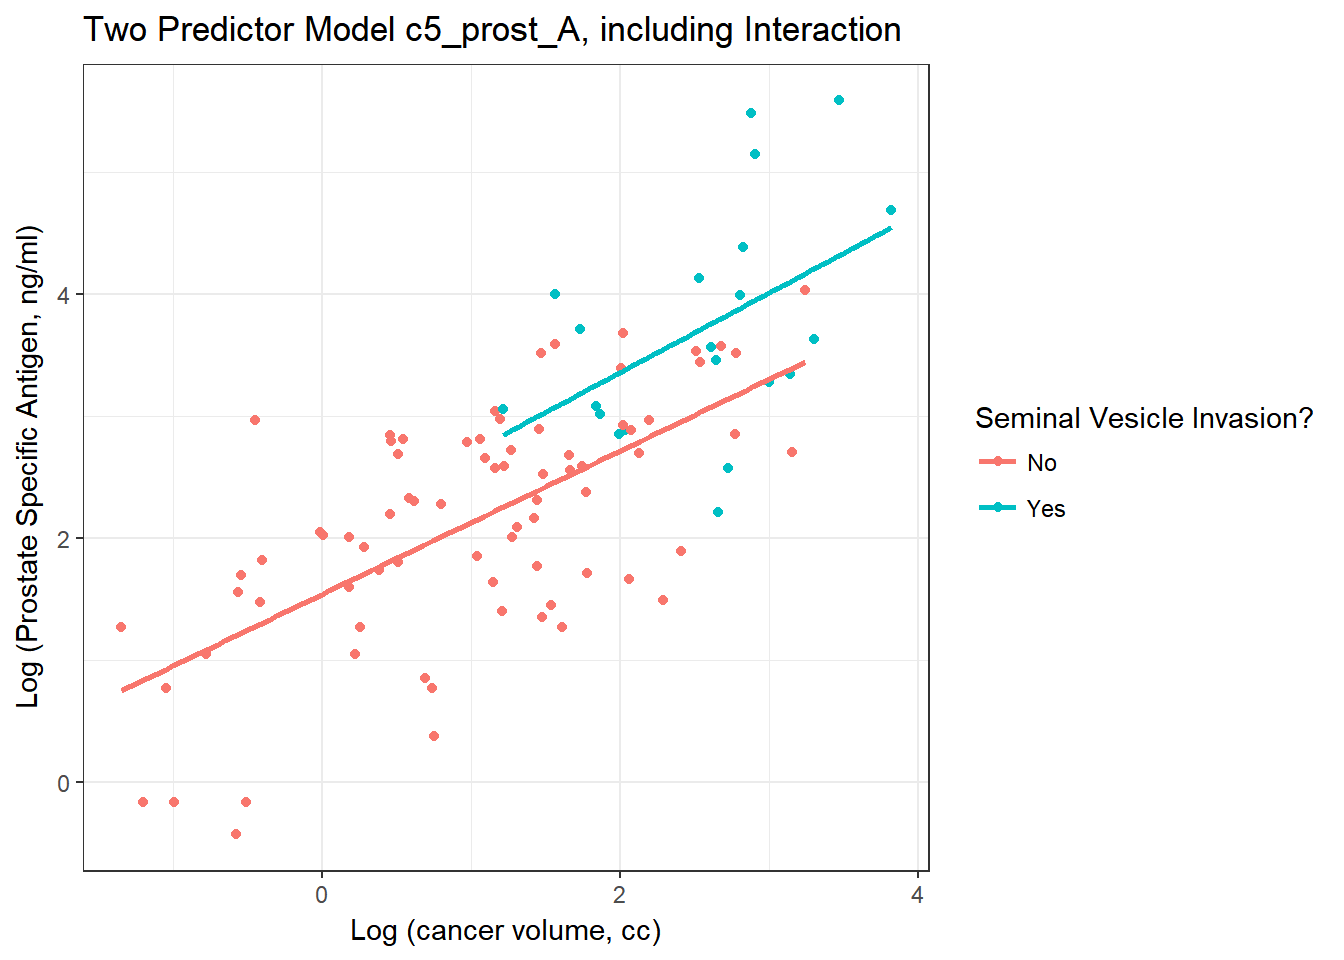
\includegraphics{bookdown-demo_files/figure-latex/unnamed-chunk-53-1.pdf}

\subsubsection{Plot on log-log scale}\label{plot-on-log-log-scale}

Another approach (which might be easier in some settings) would be to
plot the raw values of Cancer Volume and PSA, but use logarithmic axes,
again using the natural (base \emph{e}) logarithm, as follows. If we use
the default choice with `trans = ``log'', we'll find a need to select
some useful break points for the grid, as I've done in what follows.

\begin{Shaded}
\begin{Highlighting}[]
\KeywordTok{ggplot}\NormalTok{(prost, }\KeywordTok{aes}\NormalTok{(}\DataTypeTok{x =}\NormalTok{ cavol, }\DataTypeTok{y =}\NormalTok{ psa, }\DataTypeTok{group =}\NormalTok{ svi_f, }\DataTypeTok{color =}\NormalTok{ svi_f)) }\OperatorTok{+}
\StringTok{    }\KeywordTok{geom_point}\NormalTok{() }\OperatorTok{+}
\StringTok{    }\KeywordTok{geom_smooth}\NormalTok{(}\DataTypeTok{method =} \StringTok{"lm"}\NormalTok{, }\DataTypeTok{se =} \OtherTok{FALSE}\NormalTok{) }\OperatorTok{+}\StringTok{ }
\StringTok{    }\KeywordTok{scale_color_discrete}\NormalTok{(}\DataTypeTok{name =} \StringTok{"Seminal Vesicle Invasion?"}\NormalTok{) }\OperatorTok{+}
\StringTok{    }\KeywordTok{scale_x_continuous}\NormalTok{(}\DataTypeTok{trans =} \StringTok{"log"}\NormalTok{, }
                       \DataTypeTok{breaks =} \KeywordTok{c}\NormalTok{(}\FloatTok{0.5}\NormalTok{, }\DecValTok{1}\NormalTok{, }\DecValTok{2}\NormalTok{, }\DecValTok{5}\NormalTok{, }\DecValTok{10}\NormalTok{, }\DecValTok{25}\NormalTok{, }\DecValTok{50}\NormalTok{)) }\OperatorTok{+}
\StringTok{    }\KeywordTok{scale_y_continuous}\NormalTok{(}\DataTypeTok{trans =} \StringTok{"log"}\NormalTok{, }
                       \DataTypeTok{breaks =} \KeywordTok{c}\NormalTok{(}\DecValTok{1}\NormalTok{, }\DecValTok{2}\NormalTok{, }\DecValTok{4}\NormalTok{, }\DecValTok{10}\NormalTok{, }\DecValTok{25}\NormalTok{, }\DecValTok{50}\NormalTok{, }\DecValTok{100}\NormalTok{, }\DecValTok{200}\NormalTok{)) }\OperatorTok{+}
\StringTok{    }\KeywordTok{theme_bw}\NormalTok{() }\OperatorTok{+}
\StringTok{    }\KeywordTok{labs}\NormalTok{(}\DataTypeTok{x =} \StringTok{"Cancer volume, in cubic centimeters"}\NormalTok{, }
         \DataTypeTok{y =} \StringTok{"Prostate Specific Antigen, in ng/ml"}\NormalTok{, }
         \DataTypeTok{title =} \StringTok{"Two Predictor Model c5_prost_A, including Interaction"}\NormalTok{)}
\end{Highlighting}
\end{Shaded}

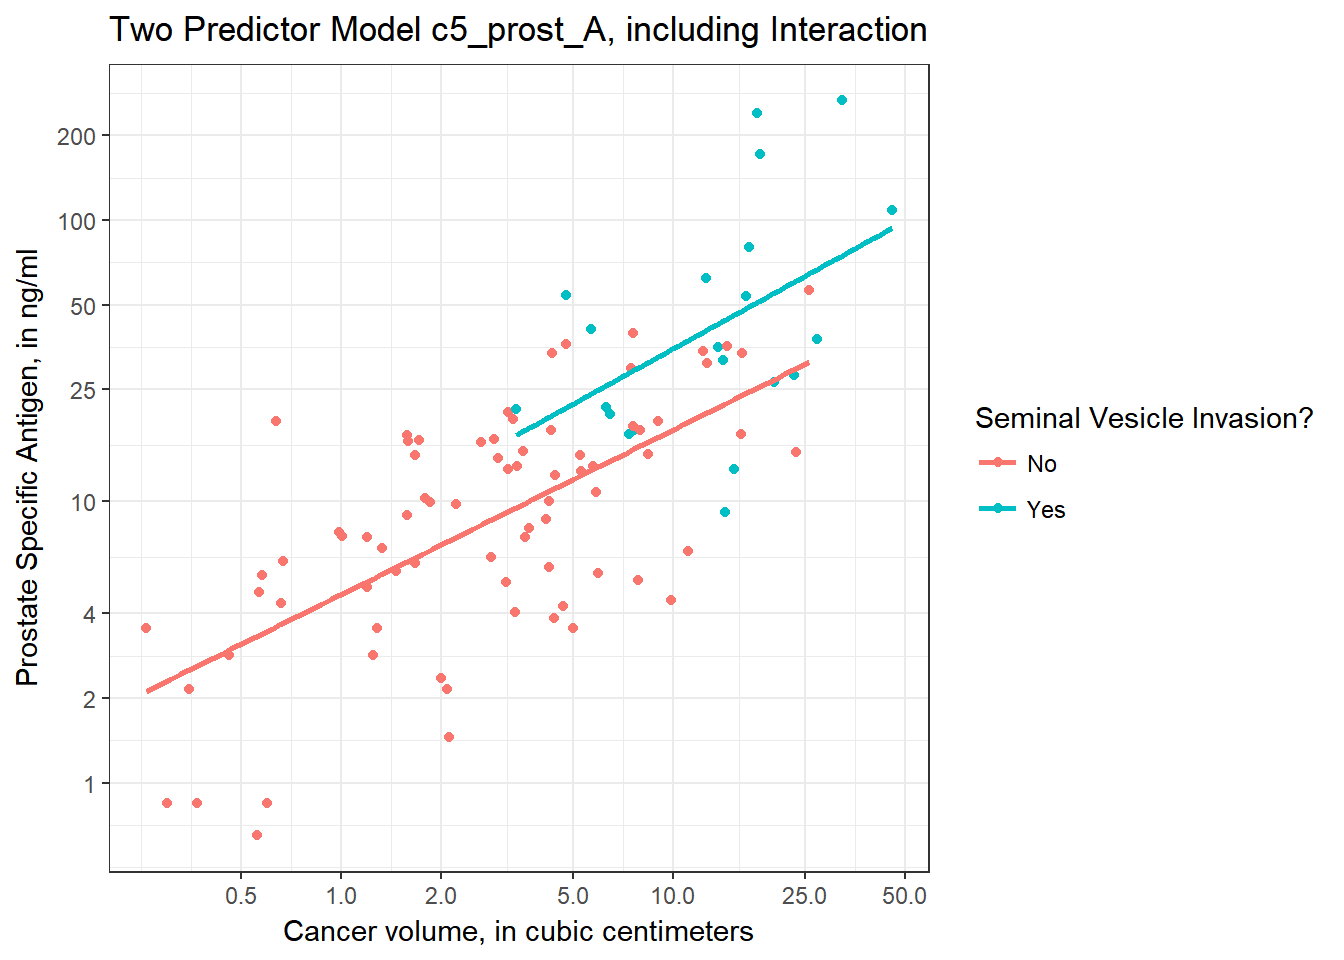
\includegraphics{bookdown-demo_files/figure-latex/unnamed-chunk-54-1.pdf}

I've used the break point of 4 on the Y axis because of the old rule
suggesting further testing for asymptomatic men with PSA of 4 or higher,
but the other break points are arbitrary - they seemed to work for me,
and used round numbers.

\subsection{\texorpdfstring{Residual Plots of
\texttt{c5\_prost\_A}}{Residual Plots of c5\_prost\_A}}\label{residual-plots-of-c5_prost_a}

\begin{Shaded}
\begin{Highlighting}[]
\KeywordTok{plot}\NormalTok{(c5_prost_A, }\DataTypeTok{which =} \DecValTok{1}\NormalTok{)}
\end{Highlighting}
\end{Shaded}

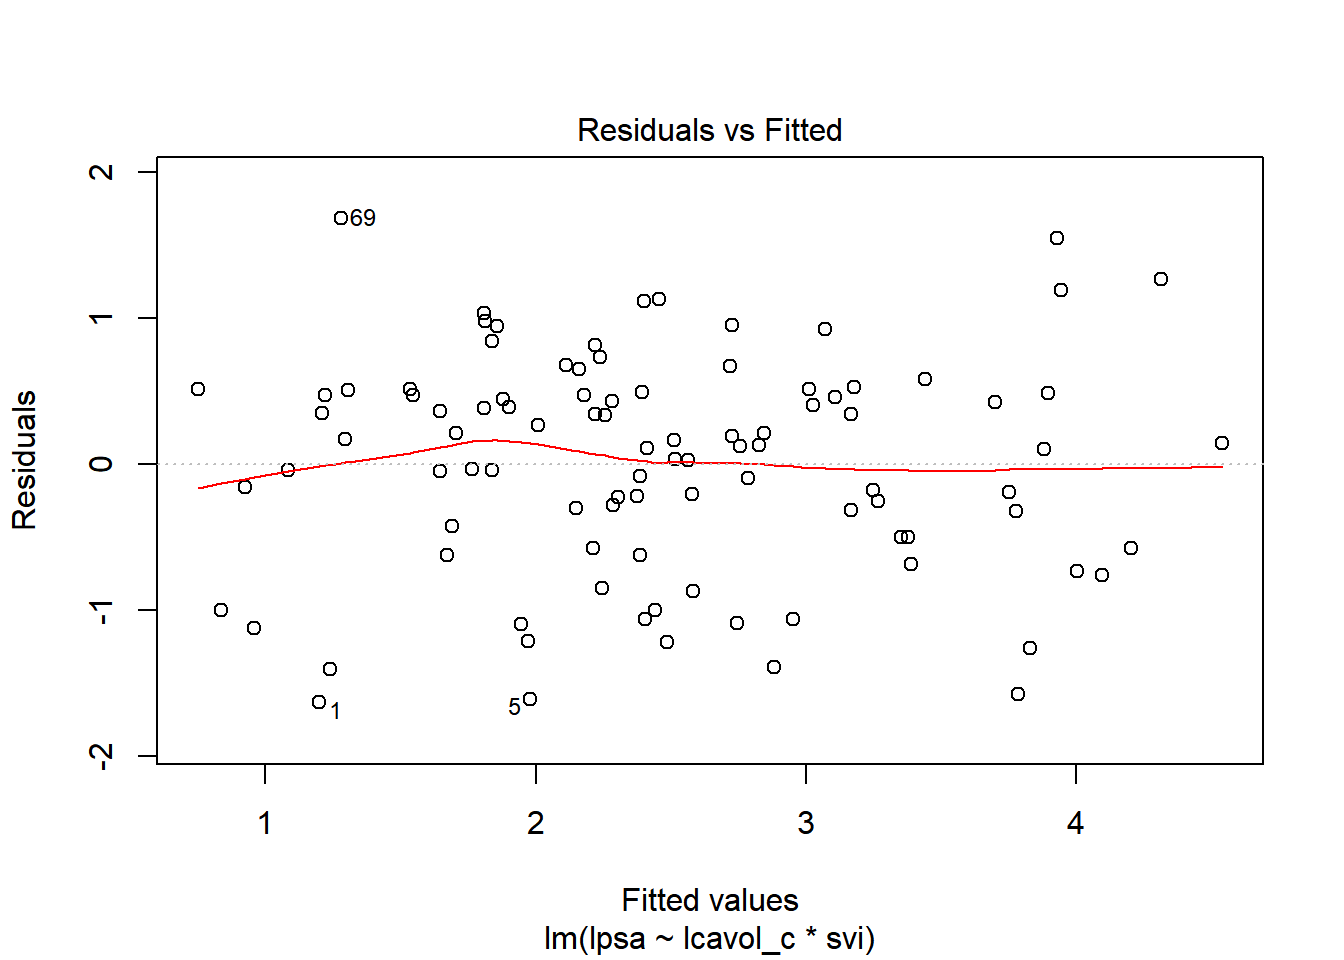
\includegraphics{bookdown-demo_files/figure-latex/unnamed-chunk-55-1.pdf}

\begin{Shaded}
\begin{Highlighting}[]
\KeywordTok{plot}\NormalTok{(c5_prost_A, }\DataTypeTok{which =} \DecValTok{5}\NormalTok{)}
\end{Highlighting}
\end{Shaded}

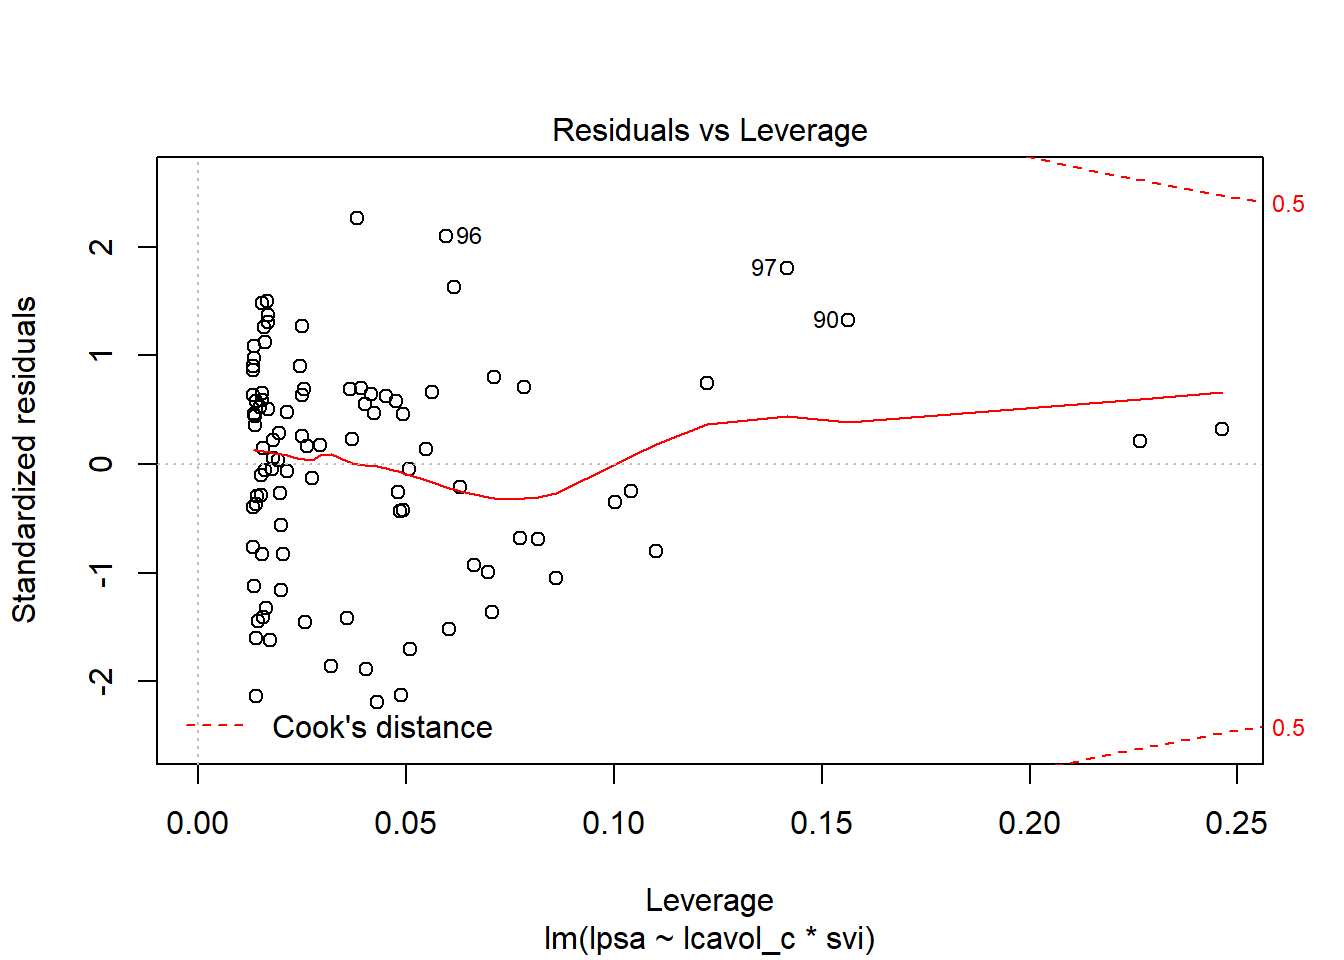
\includegraphics{bookdown-demo_files/figure-latex/unnamed-chunk-56-1.pdf}

\section{\texorpdfstring{Cross-Validation of Model
\texttt{c5\_prost\_A}}{Cross-Validation of Model c5\_prost\_A}}\label{cross-validation-of-model-c5_prost_a}

Suppose we want to evaluate whether our model \texttt{c5\_prost\_A}
predicts effectively in new data.

One approach (used, for instance, in 431) would be to split our sample
into a separate training (perhaps 70\% of the data) and test (perhaps
30\% of the data) samples, and then:

\begin{itemize}
\item
  \begin{enumerate}
  \def\labelenumi{\arabic{enumi}.}
  \tightlist
  \item
    fit the model in the training sample,
  \end{enumerate}
\item
  \begin{enumerate}
  \def\labelenumi{\arabic{enumi}.}
  \setcounter{enumi}{1}
  \tightlist
  \item
    use the resulting model to make predictions for \texttt{lpsa} in the
    test sample, and
  \end{enumerate}
\item
  \begin{enumerate}
  \def\labelenumi{\arabic{enumi}.}
  \setcounter{enumi}{2}
  \tightlist
  \item
    evaluate the quality of those predictions, perhaps by comparing the
    results to what we'd get using a different model.
  \end{enumerate}
\end{itemize}

One problem with this approach is that with a small data set like this,
we may be reluctant to cut our sample size for the training or the
testing down because we're afraid that our model building and testing
will be hampered by a small sample size. A potential solution is the
idea of \textbf{cross-validation}, which involves partitioning our data
into a series of training-test subsets, multiple times, and then
combining the results.

The rest of this section is built on some material by David Robinson at
\url{https://rpubs.com/dgrtwo/cv-modelr}.

Suppose that we want to perform what is called \emph{10-crossfold
separation}. In words, this approach splits the 97 observations in our
\texttt{prost} data frame into 10 exclusive partitions of about 90\% (so
about 87-88 observations) into a training sample, and the remaining 10\%
(9-10 observations) in a test sample\footnote{If we did 5-crossfold
  validation, we'd have 5 partitions into samples of 80\% training and
  20\% test samples.}. We then refit a model of interest using the
training data, and fit the resulting model on the test data using the
\texttt{broom} package's \texttt{augment} function. This process is then
repeated (a total of 10 times) so that each observation is used 9 times
in the training sample, and once in the test sample.

To code this in R, we'll make use of a few new ideas. Our goal will be
to cross-validate model \texttt{c5\_prost\_A}, which, you'll recall,
uses \texttt{lcavol\_c}, \texttt{svi} and their interaction, to predict
\texttt{lpsa} in the \texttt{prost} data.

\begin{enumerate}
\def\labelenumi{\arabic{enumi}.}
\tightlist
\item
  First, we set a seed for the validation algorithm, so we can replicate
  our results down the line.
\item
  Then we use the \texttt{crossv\_kfold} function from the
  \texttt{modelr} package to split the \texttt{prost} data into ten
  different partitions, and then use each partition for a split into
  training and test samples, which the machine indexes with
  \texttt{train} and \texttt{test}.
\item
  Then we use some magic and the \texttt{map} function from the
  \texttt{purrr} package (part of the core \texttt{tidyverse}) to fit a
  new \texttt{lm(lpsa\ \textasciitilde{}\ lcavol\_c\ *\ svi)} model to
  each of the training samples generated by \texttt{crossv\_kfold}.
\item
  Finally, some additional magic with the \texttt{unnest} and
  \texttt{map2} functions applies each of these new models to the
  appropriate test sample, and generate predictions (\texttt{.fitted})
  and standard errors for each prediction (\texttt{.se.fit}).
\end{enumerate}

\begin{Shaded}
\begin{Highlighting}[]
\KeywordTok{set.seed}\NormalTok{(}\DecValTok{4320308}\NormalTok{)}

\NormalTok{prost_models <-}\StringTok{ }\NormalTok{prost }\OperatorTok
\StringTok{    }\KeywordTok{crossv_kfold}\NormalTok{(}\DataTypeTok{k =} \DecValTok{10}\NormalTok{) }\OperatorTok
\StringTok{    }\KeywordTok{mutate}\NormalTok{(}\DataTypeTok{model =} \KeywordTok{map}\NormalTok{(train, }\OperatorTok{~}\StringTok{ }\KeywordTok{lm}\NormalTok{(lpsa }\OperatorTok{~}\StringTok{ }\NormalTok{lcavol_c }\OperatorTok{*}\StringTok{ }\NormalTok{svi, }\DataTypeTok{data =}\NormalTok{ .)))}

\NormalTok{prost_predictions <-}\StringTok{ }\NormalTok{prost_models }\OperatorTok
\StringTok{    }\KeywordTok{unnest}\NormalTok{(}\KeywordTok{map2}\NormalTok{(model, test, }\OperatorTok{~}\StringTok{ }\KeywordTok{augment}\NormalTok{(.x, }\DataTypeTok{newdata =}\NormalTok{ .y)))}

\KeywordTok{head}\NormalTok{(prost_predictions)}
\end{Highlighting}
\end{Shaded}

\begin{verbatim}
# A tibble: 6 x 19
  .id   subject   lpsa   lcavol lweight   age bph      svi    lcp gleason
  <chr>   <int>  <dbl>    <dbl>   <dbl> <int> <fct>  <int>  <dbl> <fct>  
1 01          3 -0.163 -0.511      2.69    74 Low        0 -1.39  7      
2 01         12  1.27  -1.35       3.60    63 Medium     0 -1.39  6      
3 01         16  1.45   1.54       3.06    66 Low        0 -1.39  6      
4 01         18  1.49   2.29       3.65    66 Low        0  0.372 6      
5 01         30  1.89   2.41       3.38    65 Low        0  1.62  6      
6 01         34  2.02   0.00995    3.27    54 Low        0 -1.39  6      
# ... with 9 more variables: pgg45 <int>, svi_f <fct>, gleason_f <fct>,
#   bph_f <fct>, lcavol_c <dbl>, cavol <dbl>, psa <dbl>, .fitted <dbl>,
#   .se.fit <dbl>
\end{verbatim}

The results are a set of predictions based on the splits into training
and test groups (remember there are 10 such splits, indexed by
\texttt{.id}) that describe the complete set of 97 subjects again.

\subsection{Cross-Validated Summaries of Prediction
Quality}\label{cross-validated-summaries-of-prediction-quality}

Now, we can calculate the root Mean Squared Prediction Error (RMSE) and
Mean Absolute Prediction Error (MAE) for this modeling approach (using
\texttt{lcavol\_c} and \texttt{svi} to predict \texttt{lpsa}) across
these observations.

\begin{Shaded}
\begin{Highlighting}[]
\NormalTok{prost_predictions }\OperatorTok
\StringTok{    }\KeywordTok{summarize}\NormalTok{(}\DataTypeTok{RMSE_ourmodel =} \KeywordTok{sqrt}\NormalTok{(}\KeywordTok{mean}\NormalTok{((lpsa }\OperatorTok{-}\StringTok{ }\NormalTok{.fitted) }\OperatorTok{^}\DecValTok{2}\NormalTok{)),}
              \DataTypeTok{MAE_ourmodel =} \KeywordTok{mean}\NormalTok{(}\KeywordTok{abs}\NormalTok{(lpsa }\OperatorTok{-}\StringTok{ }\NormalTok{.fitted)))}
\end{Highlighting}
\end{Shaded}

\begin{verbatim}
# A tibble: 1 x 2
  RMSE_ourmodel MAE_ourmodel
          <dbl>        <dbl>
1         0.783        0.638
\end{verbatim}

For now, we'll compare our model to the ``intercept only'' model that
simply predicts the mean \texttt{lpsa} across all patients.

\begin{Shaded}
\begin{Highlighting}[]
\NormalTok{prost_predictions }\OperatorTok
\StringTok{    }\KeywordTok{summarize}\NormalTok{(}\DataTypeTok{RMSE_intercept =} \KeywordTok{sqrt}\NormalTok{(}\KeywordTok{mean}\NormalTok{((lpsa }\OperatorTok{-}\StringTok{ }\KeywordTok{mean}\NormalTok{(lpsa)) }\OperatorTok{^}\DecValTok{2}\NormalTok{)),}
              \DataTypeTok{MAE_intercept =} \KeywordTok{mean}\NormalTok{(}\KeywordTok{abs}\NormalTok{(lpsa }\OperatorTok{-}\StringTok{ }\KeywordTok{mean}\NormalTok{(lpsa))))}
\end{Highlighting}
\end{Shaded}

\begin{verbatim}
# A tibble: 1 x 2
  RMSE_intercept MAE_intercept
           <dbl>         <dbl>
1           1.15         0.891
\end{verbatim}

So our model looks meaningfully better than the ``intercept only''
model, in that both the RMSE and MAE are much lower (better) with our
model.

Another thing we could do with this tibble of predictions we have
created is to graph the size of the prediction errors (observed
\texttt{lpsa} minus predicted values in \texttt{.fitted}) that our
modeling approach makes.

\begin{Shaded}
\begin{Highlighting}[]
\NormalTok{prost_predictions }\OperatorTok
\StringTok{    }\KeywordTok{mutate}\NormalTok{(}\DataTypeTok{errors =}\NormalTok{ lpsa }\OperatorTok{-}\StringTok{ }\NormalTok{.fitted) }\OperatorTok
\StringTok{    }\KeywordTok{ggplot}\NormalTok{(., }\KeywordTok{aes}\NormalTok{(}\DataTypeTok{x =}\NormalTok{ errors)) }\OperatorTok{+}
\StringTok{    }\KeywordTok{geom_histogram}\NormalTok{(}\DataTypeTok{bins =} \DecValTok{30}\NormalTok{, }\DataTypeTok{fill =} \StringTok{"darkviolet"}\NormalTok{, }\DataTypeTok{col =} \StringTok{"yellow"}\NormalTok{) }\OperatorTok{+}\StringTok{ }
\StringTok{    }\KeywordTok{labs}\NormalTok{(}\DataTypeTok{title =} \StringTok{"Cross-Validated Errors in Prediction of log(PSA)"}\NormalTok{,}
         \DataTypeTok{subtitle =} \StringTok{"Using a model (`c5_prostA`) including lcavol_c and svi and their interaction"}\NormalTok{,}
         \DataTypeTok{x =} \StringTok{"Error in predicting log(PSA)"}\NormalTok{)}
\end{Highlighting}
\end{Shaded}

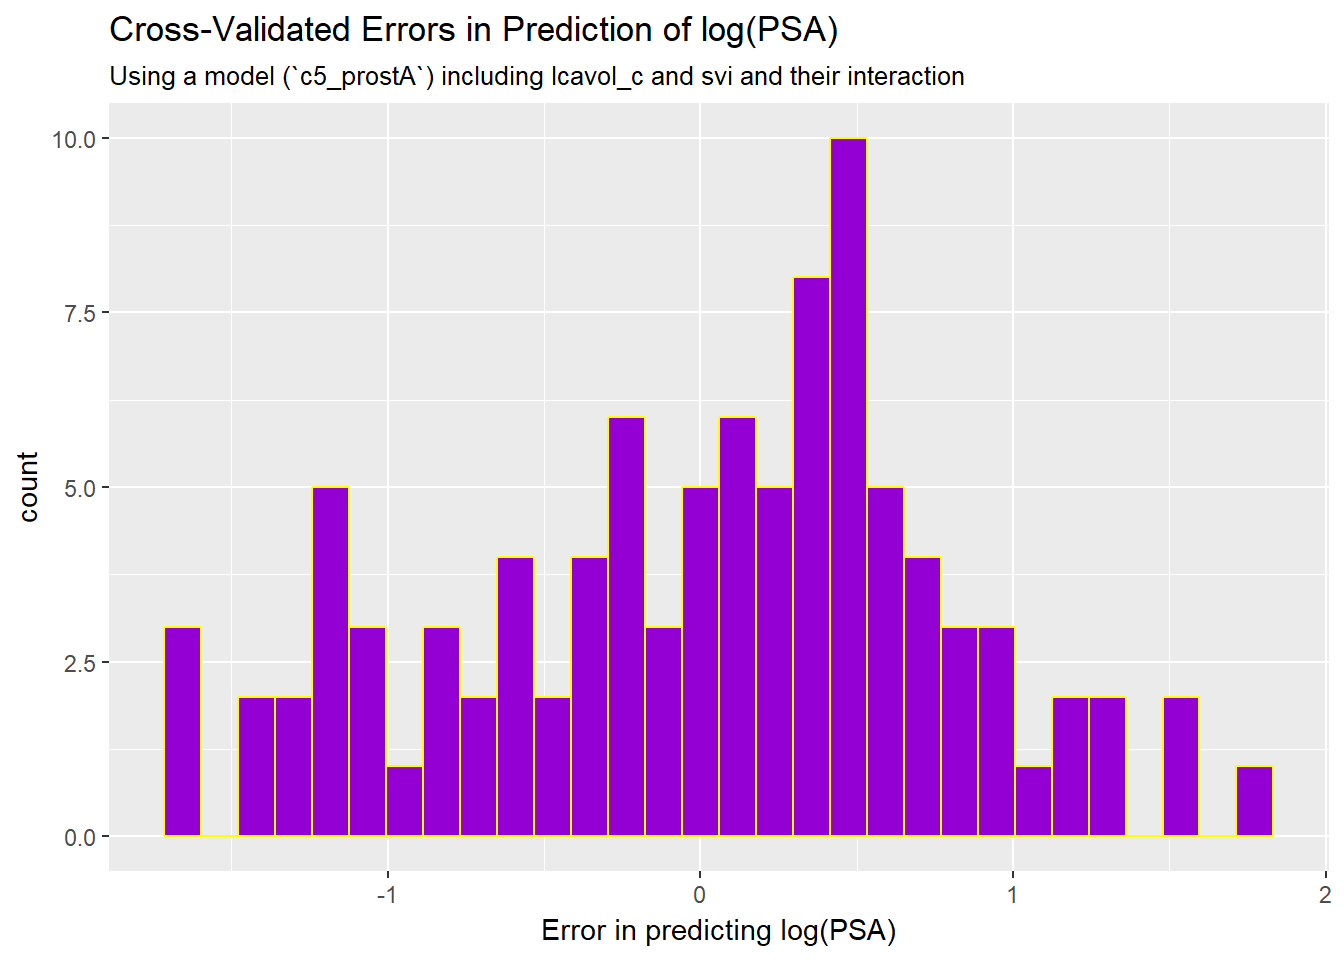
\includegraphics{bookdown-demo_files/figure-latex/validation_c5_prost_A_10fold_errors_histogram-1.pdf}

This suggests that some of our results are off by quite a bit, on the
log(PSA) scale, which is summarized for the original data below.

\begin{Shaded}
\begin{Highlighting}[]
\NormalTok{prost }\OperatorTok\StringTok{ }\KeywordTok{skim}\NormalTok{(lpsa)}
\end{Highlighting}
\end{Shaded}

\begin{verbatim}
Skim summary statistics
 n obs: 97 
 n variables: 16 

Variable type: numeric 
 variable missing complete  n mean   sd    p0  p25 median  p75 p100
     lpsa       0       97 97 2.48 1.15 -0.43 1.73   2.59 3.06 5.58
\end{verbatim}

If we like, we could transform the predictions and observed values back
to the scale of PSA (unlogged) and then calculate and display errors, as
follows:

\begin{Shaded}
\begin{Highlighting}[]
\NormalTok{prost_predictions }\OperatorTok
\StringTok{    }\KeywordTok{mutate}\NormalTok{(}\DataTypeTok{err.psa =} \KeywordTok{exp}\NormalTok{(lpsa) }\OperatorTok{-}\StringTok{ }\KeywordTok{exp}\NormalTok{(.fitted)) }\OperatorTok
\StringTok{    }\KeywordTok{ggplot}\NormalTok{(., }\KeywordTok{aes}\NormalTok{(}\DataTypeTok{x =}\NormalTok{ err.psa)) }\OperatorTok{+}
\StringTok{    }\KeywordTok{geom_histogram}\NormalTok{(}\DataTypeTok{bins =} \DecValTok{30}\NormalTok{, }\DataTypeTok{fill =} \StringTok{"darkorange"}\NormalTok{, }\DataTypeTok{col =} \StringTok{"yellow"}\NormalTok{) }\OperatorTok{+}\StringTok{ }
\StringTok{    }\KeywordTok{labs}\NormalTok{(}\DataTypeTok{title =} \StringTok{"Cross-Validated Errors in Prediction of PSA"}\NormalTok{,}
         \DataTypeTok{subtitle =} \StringTok{"Using a model (`c5_prostA`) including lcavol_c and svi and their interaction"}\NormalTok{,}
         \DataTypeTok{x =} \StringTok{"Error in predicting PSA"}\NormalTok{)}
\end{Highlighting}
\end{Shaded}

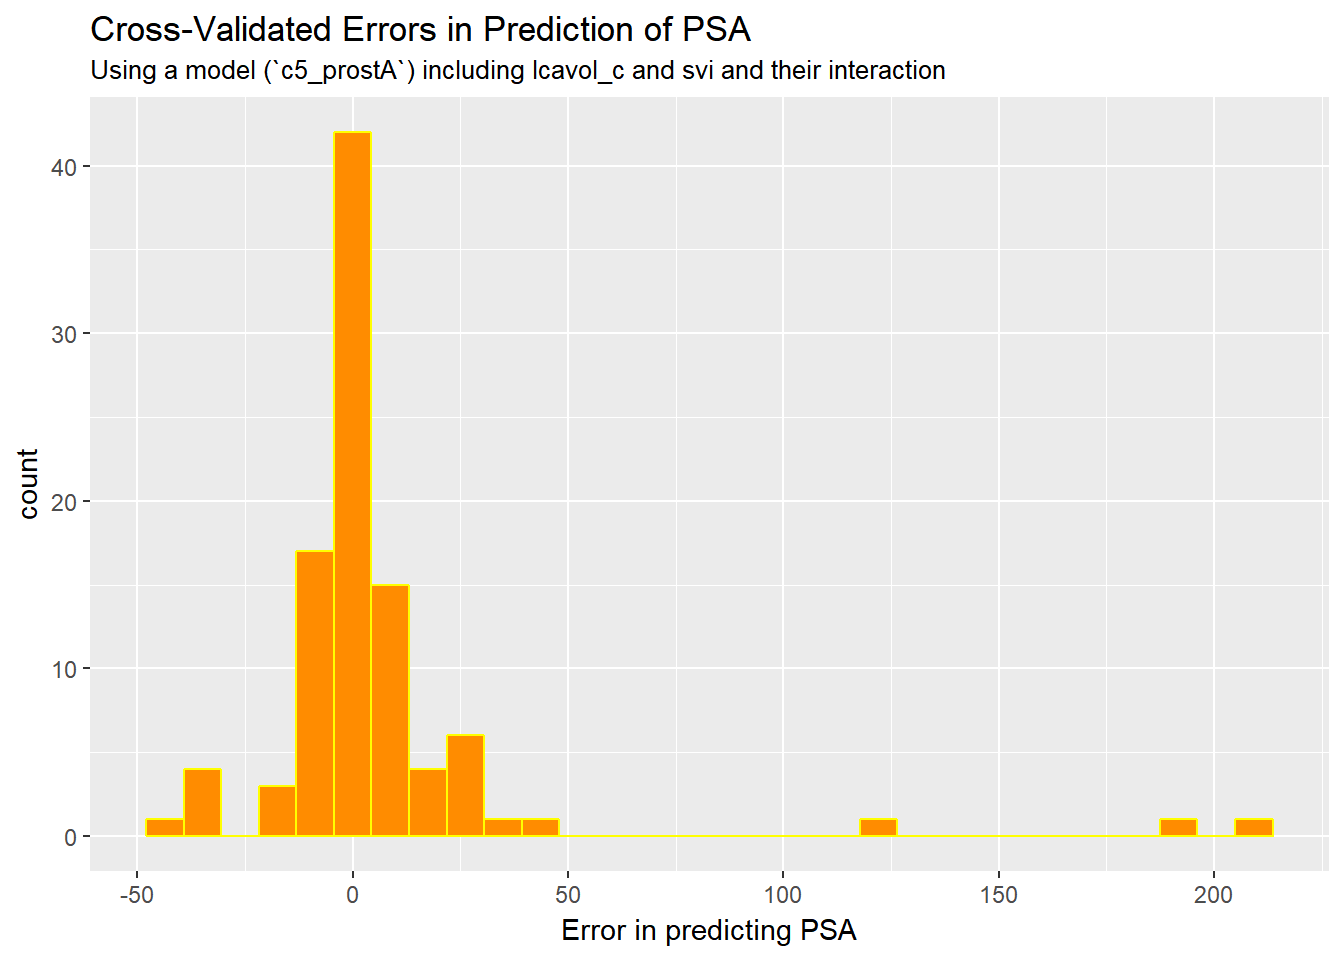
\includegraphics{bookdown-demo_files/figure-latex/validation_c5_prost_A_10fold_errorsonPSA_histogram-1.pdf}

This suggests that some of our results are off by quite a bit, on the
original scale of PSA, which is summarized below.

\begin{Shaded}
\begin{Highlighting}[]
\NormalTok{prost }\OperatorTok\StringTok{ }\KeywordTok{mutate}\NormalTok{(}\DataTypeTok{psa =} \KeywordTok{exp}\NormalTok{(lpsa)) }\OperatorTok\StringTok{ }\KeywordTok{skim}\NormalTok{(psa)}
\end{Highlighting}
\end{Shaded}

\begin{verbatim}
Skim summary statistics
 n obs: 97 
 n variables: 16 

Variable type: numeric 
 variable missing complete  n  mean    sd   p0  p25 median   p75   p100
      psa       0       97 97 23.74 40.83 0.65 5.65  13.35 21.25 265.85
\end{verbatim}

We'll return to the notion of cross-validation again, but for now, let's
consider the problem of considering adding more predictors to our model,
and then making sensible selections as to which predictors actually
should be incorporated.

\chapter{Stepwise Variable Selection}\label{stepwise-variable-selection}

\section{Strategy for Model
Selection}\label{strategy-for-model-selection}

\citet{RamseySchafer2002} suggest a strategy for dealing with many
potential explanatory variables should include the following elements:

\begin{enumerate}
\def\labelenumi{\arabic{enumi}.}
\tightlist
\item
  Identify the key objectives.
\item
  Screen the available variables, deciding on a list that is sensitive
  to the objectives and excludes obvious redundancies.
\item
  Perform exploratory analysis, examining graphical displays and
  correlation coefficients.
\item
  Perform transformations, as necessary.
\item
  Examine a residual plot after fitting a rich model, performing further
  transformations and considering outliers.
\item
  Find a suitable subset of the predictors, exerting enough control over
  any semi-automated selection procedure to be sensitive to the
  questions of interest.
\item
  Proceed with the analysis, using the selected explanatory variables.
\end{enumerate}

The Two Key Aspects of Model Selection are:

\begin{enumerate}
\def\labelenumi{\arabic{enumi}.}
\tightlist
\item
  Evaluating each potential subset of predictor variables
\item
  Deciding on the collection of potential subsets
\end{enumerate}

\subsection{How Do We Choose Potential Subsets of
Predictors?}\label{how-do-we-choose-potential-subsets-of-predictors}

Choosing potential subsets of predictor variables usually involves
either:

\begin{enumerate}
\def\labelenumi{\arabic{enumi}.}
\tightlist
\item
  Stepwise approaches
\item
  All possible subset (or best possible subset) searches
\end{enumerate}

Note that the use of any variable selection procedure changes the
properties of \ldots{}

\begin{itemize}
\tightlist
\item
  the estimated coefficients, which are biased, and
\item
  the associated tests and confidence intervals, which are overly
  optimistic.
\end{itemize}

\citet{Leeb2005} summarize the key issues:

\begin{enumerate}
\def\labelenumi{\arabic{enumi}.}
\tightlist
\item
  Regardless of sample size, the model selection step typically has a
  dramatic effect on the sampling properties of the estimators that
  cannot be ignored. In particular, the sampling properties of
  post-model-selection estimators are typically significantly different
  from the nominal distributions that arise if a fixed model is
  supposed.
\item
  As a consequence, use of inference procedures that do not take into
  account the model selection step (e.g.~using standard t-intervals as
  if the selected model has been given prior to the statistical
  analysis) can be highly misleading.
\end{enumerate}

\section{\texorpdfstring{A ``Kitchen Sink'' Model (Model
\texttt{c5\_prost\_ks})}{A Kitchen Sink Model (Model c5\_prost\_ks)}}\label{a-kitchen-sink-model-model-c5_prost_ks}

Suppose that we now consider a model for the \texttt{prost} data we have
been working with, which includes main effects (and, in this case, only
the main effects) of all eight candidate predictors for \texttt{lpsa},
as follows.

\begin{Shaded}
\begin{Highlighting}[]
\NormalTok{c5_prost_ks <-}\StringTok{ }\KeywordTok{lm}\NormalTok{(lpsa }\OperatorTok{~}\StringTok{ }\NormalTok{lcavol }\OperatorTok{+}\StringTok{ }\NormalTok{lweight }\OperatorTok{+}\StringTok{ }\NormalTok{age }\OperatorTok{+}\StringTok{ }\NormalTok{bph_f }\OperatorTok{+}\StringTok{ }\NormalTok{svi_f }\OperatorTok{+}\StringTok{ }
\StringTok{                }\NormalTok{lcp }\OperatorTok{+}\StringTok{ }\NormalTok{gleason_f }\OperatorTok{+}\StringTok{ }\NormalTok{pgg45, }\DataTypeTok{data =}\NormalTok{ prost)}

\KeywordTok{tidy}\NormalTok{(c5_prost_ks)}
\end{Highlighting}
\end{Shaded}

\begin{verbatim}
          term     estimate   std.error  statistic      p.value
1  (Intercept)  0.169937821 0.931332512  0.1824674 8.556454e-01
2       lcavol  0.544313829 0.087979210  6.1868461 2.010505e-08
3      lweight  0.702237531 0.203013089  3.4590751 8.455164e-04
4          age -0.023857982 0.011081414 -2.1529727 3.412099e-02
5  bph_fMedium  0.364036274 0.182575941  1.9938896 4.933267e-02
6    bph_fHigh  0.248789989 0.195975792  1.2694935 2.076898e-01
7     svi_fYes  0.710949408 0.241990241  2.9379259 4.240326e-03
8          lcp -0.119311781 0.089458946 -1.3337043 1.858223e-01
9   gleason_f7  0.220746268 0.343065609  0.6434520 5.216430e-01
10  gleason_f6 -0.053096704 0.430098039 -0.1234526 9.020368e-01
11       pgg45  0.003984574 0.004146495  0.9609499 3.392714e-01
\end{verbatim}

\begin{Shaded}
\begin{Highlighting}[]
\KeywordTok{glance}\NormalTok{(c5_prost_ks)}
\end{Highlighting}
\end{Shaded}

\begin{verbatim}
  r.squared adj.r.squared     sigma statistic      p.value df    logLik
1 0.6790343     0.6417127 0.6909479  18.19414 2.373796e-17 11 -95.93939
       AIC      BIC deviance df.residual
1 215.8788 246.7753 41.05718          86
\end{verbatim}

We'll often refer to this (all predictors on board) approach as a
``kitchen sink'' model{[}This refers to the English idiom ``\ldots{}
everything but the kitchen sink'' which describes, essentially,
everything imaginable. A ``kitchen sink regression'' is often used as a
pejorative term, since no special skill or insight is required to
identify it, given a list of potential predictors. For more, yes, there
is a
\href{https://en.wikipedia.org/wiki/Kitchen_sink_regression}{Wikipedia
page}.{]}.

\section{Sequential Variable Selection: Stepwise
Approaches}\label{sequential-variable-selection-stepwise-approaches}

\begin{itemize}
\tightlist
\item
  Forward Selection

  \begin{itemize}
  \tightlist
  \item
    We begin with a constant mean and then add potential predictors one
    at a time according to some criterion (R defaults to minimizing the
    Akaike Information Criterion) until no further addition
    significantly improves the fit.
  \item
    Each categorical factor variable is represented in the regression
    model as a set of indicator variables. In the absence of a good
    reason to do something else, the set is added to the model as a
    single unit, and R does this automatically.
  \end{itemize}
\item
  Backwards Elimination

  \begin{itemize}
  \tightlist
  \item
    Start with the ``kitchen sink'' model and then delete potential
    predictors one at a time.
  \item
    Backwards Elimination is less likely than Forward Selection, to omit
    negatively confounded sets of variables, though all stepwise
    procedures have problems.
  \end{itemize}
\item
  Stepwise Regression can also be done by combining these methods.
\end{itemize}

\subsection{The Big Problems with Stepwise
Regression}\label{the-big-problems-with-stepwise-regression}

There is no reason to assume that a single best model can be found.

\begin{itemize}
\tightlist
\item
  The use of forward selection, or backwards elimination, or stepwise
  regression including both procedures, will NOT always find the same
  model.
\item
  It also appears to be essentially useless to try different stepwise
  methods to look for agreement.
\end{itemize}

Users of stepwise regression frequently place all of their attention on
the particular explanatory variables included in the resulting model,
when there's \textbf{no reason} (in most cases) to assume that model is
in any way optimal.

Despite all of its problems, let's use stepwise regression to help
predict \texttt{lpsa} given a subset of the eight predictors in
\texttt{c5\_prost\_ks}.

\section{\texorpdfstring{Forward Selection with the \texttt{step}
function}{Forward Selection with the step function}}\label{forward-selection-with-the-step-function}

\begin{enumerate}
\def\labelenumi{\arabic{enumi}.}
\tightlist
\item
  Specify the null model (intercept only)
\item
  Specify the variables R should consider as predictors (in the scope
  element of the step function)
\item
  Specify forward selection only
\item
  R defaults to using AIC as its stepwise criterion
\end{enumerate}

\begin{Shaded}
\begin{Highlighting}[]
\KeywordTok{with}\NormalTok{(prost, }
     \KeywordTok{step}\NormalTok{(}\KeywordTok{lm}\NormalTok{(lpsa }\OperatorTok{~}\StringTok{ }\DecValTok{1}\NormalTok{), }
     \DataTypeTok{scope=}\NormalTok{(}\OperatorTok{~}\StringTok{ }\NormalTok{lcavol }\OperatorTok{+}\StringTok{ }\NormalTok{lweight }\OperatorTok{+}\StringTok{ }\NormalTok{age }\OperatorTok{+}\StringTok{ }\NormalTok{bph_f }\OperatorTok{+}\StringTok{ }\NormalTok{svi_f }\OperatorTok{+}\StringTok{ }
\StringTok{                }\NormalTok{lcp }\OperatorTok{+}\StringTok{ }\NormalTok{gleason_f }\OperatorTok{+}\StringTok{ }\NormalTok{pgg45), }
     \DataTypeTok{direction=}\StringTok{"forward"}\NormalTok{))}
\end{Highlighting}
\end{Shaded}

\begin{verbatim}
Start:  AIC=28.84
lpsa ~ 1

            Df Sum of Sq     RSS     AIC
+ lcavol     1    69.003  58.915 -44.366
+ svi_f      1    41.011  86.907  -6.658
+ lcp        1    38.528  89.389  -3.926
+ gleason_f  2    30.121  97.796   6.793
+ lweight    1    24.019 103.899  10.665
+ pgg45      1    22.814 105.103  11.783
+ age        1     3.679 124.239  28.007
<none>                   127.918  28.838
+ bph_f      2     4.681 123.237  29.221

Step:  AIC=-44.37
lpsa ~ lcavol

            Df Sum of Sq    RSS     AIC
+ lweight    1    7.1726 51.742 -54.958
+ svi_f      1    5.2375 53.677 -51.397
+ bph_f      2    3.2994 55.615 -45.956
+ pgg45      1    1.6980 57.217 -45.203
+ gleason_f  2    2.7834 56.131 -45.061
<none>                   58.915 -44.366
+ lcp        1    0.6562 58.259 -43.452
+ age        1    0.0025 58.912 -42.370

Step:  AIC=-54.96
lpsa ~ lcavol + lweight

            Df Sum of Sq    RSS     AIC
+ svi_f      1    5.1737 46.568 -63.177
+ pgg45      1    1.8158 49.926 -56.424
+ gleason_f  2    2.6770 49.065 -56.111
<none>                   51.742 -54.958
+ lcp        1    0.8187 50.923 -54.506
+ age        1    0.6456 51.097 -54.176
+ bph_f      2    1.4583 50.284 -53.731

Step:  AIC=-63.18
lpsa ~ lcavol + lweight + svi_f

            Df Sum of Sq    RSS     AIC
<none>                   46.568 -63.177
+ gleason_f  2   1.60467 44.964 -62.579
+ age        1   0.62301 45.945 -62.484
+ bph_f      2   1.50046 45.068 -62.354
+ pgg45      1   0.50069 46.068 -62.226
+ lcp        1   0.06937 46.499 -61.322
\end{verbatim}

\begin{verbatim}

Call:
lm(formula = lpsa ~ lcavol + lweight + svi_f)

Coefficients:
(Intercept)       lcavol      lweight     svi_fYes  
    -0.7772       0.5259       0.6618       0.6657  
\end{verbatim}

The resulting model, arrived at after three forward selection steps,
includes \texttt{lcavol}, \texttt{lweight} and \texttt{svi\_f}.

\begin{Shaded}
\begin{Highlighting}[]
\NormalTok{model.fs <-}\StringTok{ }\KeywordTok{lm}\NormalTok{(lpsa }\OperatorTok{~}\StringTok{ }\NormalTok{lcavol }\OperatorTok{+}\StringTok{ }\NormalTok{lweight }\OperatorTok{+}\StringTok{ }\NormalTok{svi_f, }
               \DataTypeTok{data=}\NormalTok{prost)}
\KeywordTok{summary}\NormalTok{(model.fs)}\OperatorTok{$}\NormalTok{adj.r.squared}
\end{Highlighting}
\end{Shaded}

\begin{verbatim}
[1] 0.6242063
\end{verbatim}

\begin{Shaded}
\begin{Highlighting}[]
\KeywordTok{extractAIC}\NormalTok{(model.fs)}
\end{Highlighting}
\end{Shaded}

\begin{verbatim}
[1]   4.00000 -63.17744
\end{verbatim}

The adjusted R\textsuperscript{2} value for this model is 0.624, and the
AIC value used by the stepwise procedure is -63.18, on 4 effective
degrees of freedom.

\section{\texorpdfstring{Backward Elimination using the \texttt{step}
function}{Backward Elimination using the step function}}\label{backward-elimination-using-the-step-function}

In this case, the backward elimination approach, using reduction in AIC
for a criterion, comes to the same conclusion about the ``best'' model.

\begin{Shaded}
\begin{Highlighting}[]
\KeywordTok{with}\NormalTok{(prost, }
     \KeywordTok{step}\NormalTok{(}\KeywordTok{lm}\NormalTok{(lpsa }\OperatorTok{~}\StringTok{ }\NormalTok{lcavol }\OperatorTok{+}\StringTok{ }\NormalTok{lweight }\OperatorTok{+}\StringTok{ }\NormalTok{age }\OperatorTok{+}\StringTok{ }\NormalTok{bph_f }\OperatorTok{+}\StringTok{ }
\StringTok{                 }\NormalTok{svi_f }\OperatorTok{+}\StringTok{ }\NormalTok{lcp }\OperatorTok{+}\StringTok{ }\NormalTok{gleason_f }\OperatorTok{+}\StringTok{ }\NormalTok{pgg45), }
          \DataTypeTok{direction=}\StringTok{"backward"}\NormalTok{))}
\end{Highlighting}
\end{Shaded}

\begin{verbatim}
Start:  AIC=-61.4
lpsa ~ lcavol + lweight + age + bph_f + svi_f + lcp + gleason_f + 
    pgg45

            Df Sum of Sq    RSS     AIC
- gleason_f  2    1.1832 42.240 -62.639
- pgg45      1    0.4409 41.498 -62.359
- lcp        1    0.8492 41.906 -61.409
<none>                   41.057 -61.395
- bph_f      2    2.0299 43.087 -60.714
- age        1    2.2129 43.270 -58.303
- svi_f      1    4.1207 45.178 -54.118
- lweight    1    5.7123 46.769 -50.760
- lcavol     1   18.2738 59.331 -27.683

Step:  AIC=-62.64
lpsa ~ lcavol + lweight + age + bph_f + svi_f + lcp + pgg45

          Df Sum of Sq    RSS     AIC
- lcp      1    0.8470 43.087 -62.713
<none>                 42.240 -62.639
- pgg45    1    1.2029 43.443 -61.916
- bph_f    2    2.2515 44.492 -61.602
- age      1    2.0730 44.313 -59.992
- svi_f    1    4.6431 46.884 -54.523
- lweight  1    5.5988 47.839 -52.566
- lcavol   1   21.4956 63.736 -24.736

Step:  AIC=-62.71
lpsa ~ lcavol + lweight + age + bph_f + svi_f + pgg45

          Df Sum of Sq    RSS     AIC
- pgg45    1    0.5860 43.673 -63.403
<none>                 43.087 -62.713
- bph_f    2    2.0214 45.109 -62.266
- age      1    1.7101 44.798 -60.938
- svi_f    1    3.7964 46.884 -56.523
- lweight  1    5.6462 48.734 -52.769
- lcavol   1   22.5152 65.603 -23.936

Step:  AIC=-63.4
lpsa ~ lcavol + lweight + age + bph_f + svi_f

          Df Sum of Sq    RSS     AIC
<none>                 43.673 -63.403
- bph_f    2    2.2720 45.945 -62.484
- age      1    1.3945 45.068 -62.354
- svi_f    1    5.2747 48.948 -54.343
- lweight  1    5.3319 49.005 -54.230
- lcavol   1   25.5538 69.227 -20.720
\end{verbatim}

\begin{verbatim}

Call:
lm(formula = lpsa ~ lcavol + lweight + age + bph_f + svi_f)

Coefficients:
(Intercept)       lcavol      lweight          age  bph_fMedium  
    0.14329      0.54022      0.67283     -0.01819      0.37607  
  bph_fHigh     svi_fYes  
    0.27216      0.68174  
\end{verbatim}

The backwards elimination approach in this case lands on a model with
five inputs (one of which includes two \texttt{bph} indicators,)
eliminating only \texttt{gleason\_f}, \texttt{pgg45} and \texttt{lcp}.

\section{Allen-Cady Modified Backward
Elimination}\label{allen-cady-modified-backward-elimination}

Ranking candidate predictors by importance in advance of backwards
elimination can help avoid false-positives, while reducing model size.
See \citet{Vittinghoff2012}, Section 10.3 for more details.

\begin{enumerate}
\def\labelenumi{\arabic{enumi}.}
\tightlist
\item
  First, force into the model any predictors of primary interest, and
  any confounders necessary for face validity of the final model.

  \begin{itemize}
  \tightlist
  \item
    ``Some variables in the hypothesized causal model may be such
    well-established causal antecedents of the outcome that it makes
    sense to include them, essentially to establish the face validity of
    the model and without regard to the strength or statistical
    significance of their associations with the primary predictor and
    outcome \ldots{}''
  \end{itemize}
\item
  Rank the remaining candidate predictors in order of importance.
\item
  Starting from an initial model with all candidate predictors included,
  delete predictors in order of ascending importance until the first
  variable meeting a criterion to stay in the model hits. Then stop.
\end{enumerate}

Only the remaining variable hypothesized to be least important is
eligible for removal at each step. When we are willing to do this
sorting before collecting (or analyzing) the data, then we can do
Allen-Cady backwards elimination using the \texttt{drop1} command in R.

\subsection{Demonstration of the Allen-Cady
approach}\label{demonstration-of-the-allen-cady-approach}

Suppose, for the moment that we decided to fit a model for the log of
\texttt{psa} and we decided (before we saw the data) that we would:

lcavol + lweight + svi\_f + age + bph\_f + gleason\_f + lcp + pgg45

\begin{itemize}
\tightlist
\item
  force the \texttt{gleason\_f} variable to be in the model, due to
  prior information about its importance,
\item
  and then rated the importance of the other variables as
  \texttt{lcavol} (most important), then \texttt{svi\_f} then
  \texttt{age}, and then \texttt{bph\_f}, then \texttt{lweight} and
  \texttt{lcp} followed by \texttt{pgg45} (least important)
\end{itemize}

When we are willing to do this sorting before collecting (or analyzing)
the data, then we can do Allen-Cady backwards elimination using the
\texttt{drop1} command in R.

\textbf{Step 1.} Fit the full model, then see if removing \texttt{pgg45}
improves AIC\ldots{}

\begin{Shaded}
\begin{Highlighting}[]
\KeywordTok{with}\NormalTok{(prost, }\KeywordTok{drop1}\NormalTok{(}\KeywordTok{lm}\NormalTok{(lpsa }\OperatorTok{~}\StringTok{ }\NormalTok{gleason_f }\OperatorTok{+}\StringTok{ }\NormalTok{lcavol }\OperatorTok{+}\StringTok{ }\NormalTok{svi_f }\OperatorTok{+}\StringTok{ }
\StringTok{              }\NormalTok{age }\OperatorTok{+}\StringTok{ }\NormalTok{bph_f }\OperatorTok{+}\StringTok{ }\NormalTok{lweight }\OperatorTok{+}\StringTok{ }\NormalTok{lcp }\OperatorTok{+}\StringTok{ }\NormalTok{pgg45),}
              \DataTypeTok{scope =}\NormalTok{ (}\OperatorTok{~}\StringTok{ }\NormalTok{pgg45)))}
\end{Highlighting}
\end{Shaded}

\begin{verbatim}
Single term deletions

Model:
lpsa ~ gleason_f + lcavol + svi_f + age + bph_f + lweight + lcp + 
    pgg45
       Df Sum of Sq    RSS     AIC
<none>              41.057 -61.395
pgg45   1   0.44085 41.498 -62.359
\end{verbatim}

Since -62.3 is smaller (i.e.~more negative) than -61.4, we delete
\texttt{pgg45} and move on to assess whether we can remove the variable
we deemed next least important (\texttt{lcp})

\textbf{Step 2.} Let's see if removing \texttt{lcp} from this model
improves AIC\ldots{}

\begin{Shaded}
\begin{Highlighting}[]
\KeywordTok{with}\NormalTok{(prost, }\KeywordTok{drop1}\NormalTok{(}\KeywordTok{lm}\NormalTok{(lpsa }\OperatorTok{~}\StringTok{ }\NormalTok{gleason_f }\OperatorTok{+}\StringTok{ }\NormalTok{lcavol }\OperatorTok{+}\StringTok{ }\NormalTok{svi_f }\OperatorTok{+}\StringTok{ }
\StringTok{              }\NormalTok{age }\OperatorTok{+}\StringTok{ }\NormalTok{bph_f }\OperatorTok{+}\StringTok{ }\NormalTok{lweight  }\OperatorTok{+}\StringTok{ }\NormalTok{lcp),}
              \DataTypeTok{scope =}\NormalTok{ (}\OperatorTok{~}\StringTok{ }\NormalTok{lcp)))}
\end{Highlighting}
\end{Shaded}

\begin{verbatim}
Single term deletions

Model:
lpsa ~ gleason_f + lcavol + svi_f + age + bph_f + lweight + lcp
       Df Sum of Sq    RSS     AIC
<none>              41.498 -62.359
lcp     1   0.56767 42.066 -63.041
\end{verbatim}

Again, since -63.0 is smaller than -62.4, we delete \texttt{lcp} and
next assess whether we should delete \texttt{lweight}.

\textbf{Step 3.} Does removing \texttt{lweight} from this model improves
AIC\ldots{}

\begin{Shaded}
\begin{Highlighting}[]
\KeywordTok{with}\NormalTok{(prost, }\KeywordTok{drop1}\NormalTok{(}\KeywordTok{lm}\NormalTok{(lpsa }\OperatorTok{~}\StringTok{ }\NormalTok{gleason_f }\OperatorTok{+}\StringTok{ }\NormalTok{lcavol }\OperatorTok{+}\StringTok{ }\NormalTok{svi_f }\OperatorTok{+}\StringTok{ }
\StringTok{              }\NormalTok{age }\OperatorTok{+}\StringTok{ }\NormalTok{bph_f }\OperatorTok{+}\StringTok{ }\NormalTok{lweight),}
              \DataTypeTok{scope =}\NormalTok{ (}\OperatorTok{~}\StringTok{ }\NormalTok{lweight)))}
\end{Highlighting}
\end{Shaded}

\begin{verbatim}
Single term deletions

Model:
lpsa ~ gleason_f + lcavol + svi_f + age + bph_f + lweight
        Df Sum of Sq    RSS     AIC
<none>               42.066 -63.041
lweight  1     5.678 47.744 -52.760
\end{verbatim}

Since the AIC for the model after the removal of \texttt{lweight} is
larger (i.e.~less negative), we stop, and declare our final model by the
Allen-Cady approach to include \texttt{gleason\_f}, \texttt{lcavol},
\texttt{svi\_f}, \texttt{age}, \texttt{bph\_f} and \texttt{lweight}.

\section{Summarizing the Results}\label{summarizing-the-results}

\begin{longtable}[]{@{}rl@{}}
\toprule
Method & Suggested Predictors\tabularnewline
\midrule
\endhead
Forward selection & \texttt{lcavol}, \texttt{lweight},
\texttt{svi\_f}\tabularnewline
Backwards elimination & \texttt{lcavol}, \texttt{lweight},
\texttt{svi\_f}, \texttt{age}, \texttt{bph\_f}\tabularnewline
Allen-Cady approach & \texttt{lcavol}, \texttt{lweight},
\texttt{svi\_f}, \texttt{age}, \texttt{bph\_f},
\texttt{gleason\_f}\tabularnewline
\bottomrule
\end{longtable}

\subsection{In-Sample Testing and
Summaries}\label{in-sample-testing-and-summaries}

Since these models are nested in each other, let's look at the summary
statistics (like R\textsuperscript{2}, and AIC) and also run an
ANOVA-based comparison of these nested models to each other and to the
model with the intercept alone, and the kitchen sink model with all
available predictors.

\begin{Shaded}
\begin{Highlighting}[]
\NormalTok{prost_m_int <-}\StringTok{ }\KeywordTok{lm}\NormalTok{(lpsa }\OperatorTok{~}\StringTok{ }\DecValTok{1}\NormalTok{, }\DataTypeTok{data =}\NormalTok{ prost)}
\NormalTok{prost_m_fw <-}\StringTok{ }\KeywordTok{lm}\NormalTok{(lpsa }\OperatorTok{~}\StringTok{ }\NormalTok{lcavol }\OperatorTok{+}\StringTok{ }\NormalTok{lweight }\OperatorTok{+}\StringTok{ }\NormalTok{svi_f, }\DataTypeTok{data =}\NormalTok{ prost)}
\NormalTok{prost_m_bw <-}\StringTok{ }\KeywordTok{lm}\NormalTok{(lpsa }\OperatorTok{~}\StringTok{ }\NormalTok{lcavol }\OperatorTok{+}\StringTok{ }\NormalTok{lweight }\OperatorTok{+}\StringTok{ }\NormalTok{svi_f }\OperatorTok{+}\StringTok{ }
\StringTok{              }\NormalTok{age }\OperatorTok{+}\StringTok{ }\NormalTok{bph_f }\OperatorTok{+}\StringTok{ }\NormalTok{gleason_f, }\DataTypeTok{data =}\NormalTok{ prost)}
\NormalTok{prost_m_ac <-}\StringTok{ }\KeywordTok{lm}\NormalTok{(lpsa }\OperatorTok{~}\StringTok{ }\NormalTok{lcavol }\OperatorTok{+}\StringTok{ }\NormalTok{lweight }\OperatorTok{+}\StringTok{ }\NormalTok{svi_f }\OperatorTok{+}\StringTok{ }
\StringTok{              }\NormalTok{age }\OperatorTok{+}\StringTok{ }\NormalTok{bph_f }\OperatorTok{+}\StringTok{ }\NormalTok{gleason_f }\OperatorTok{+}\StringTok{ }\NormalTok{lcp, }\DataTypeTok{data =}\NormalTok{ prost)}
\NormalTok{prost_m_ks <-}\StringTok{ }\KeywordTok{lm}\NormalTok{(lpsa }\OperatorTok{~}\StringTok{ }\NormalTok{lcavol }\OperatorTok{+}\StringTok{ }\NormalTok{lweight }\OperatorTok{+}\StringTok{ }\NormalTok{svi_f }\OperatorTok{+}\StringTok{ }
\StringTok{              }\NormalTok{age }\OperatorTok{+}\StringTok{ }\NormalTok{bph_f }\OperatorTok{+}\StringTok{ }\NormalTok{gleason_f }\OperatorTok{+}\StringTok{ }\NormalTok{lcp }\OperatorTok{+}\StringTok{ }\NormalTok{pgg45, }\DataTypeTok{data =}\NormalTok{ prost)}
\end{Highlighting}
\end{Shaded}

\subsubsection{\texorpdfstring{Model Fit Summaries (in-sample) from
\texttt{glance}}{Model Fit Summaries (in-sample) from glance}}\label{model-fit-summaries-in-sample-from-glance}

Here are the models, at a \texttt{glance} from the \texttt{broom}
package.

\begin{Shaded}
\begin{Highlighting}[]
\NormalTok{prost_sum <-}\StringTok{ }\KeywordTok{bind_rows}\NormalTok{(}\KeywordTok{glance}\NormalTok{(prost_m_int), }\KeywordTok{glance}\NormalTok{(prost_m_fw),}
                       \KeywordTok{glance}\NormalTok{(prost_m_bw), }\KeywordTok{glance}\NormalTok{(prost_m_ac), }
                       \KeywordTok{glance}\NormalTok{(prost_m_ks)) }\OperatorTok\StringTok{ }\KeywordTok{round}\NormalTok{(., }\DecValTok{3}\NormalTok{)}
\NormalTok{prost_sum}\OperatorTok{$}\NormalTok{names <-}\StringTok{ }\KeywordTok{c}\NormalTok{(}\StringTok{"intercept"}\NormalTok{, }\StringTok{"lcavol + lweight + svi"}\NormalTok{, }
                      \StringTok{"... + age + bhp + gleason"}\NormalTok{, }\StringTok{"... + lcp"}\NormalTok{, }\StringTok{"... + pgg45"}\NormalTok{)}
\NormalTok{prost_sum <-}\StringTok{ }\NormalTok{prost_sum }\OperatorTok
\StringTok{    }\KeywordTok{select}\NormalTok{(names, r.squared, adj.r.squared, AIC, BIC, sigma, df, df.residual)}

\NormalTok{prost_sum}
\end{Highlighting}
\end{Shaded}

\begin{verbatim}
                      names r.squared adj.r.squared     AIC     BIC sigma
1                 intercept     0.000         0.000 306.112 311.261 1.154
2    lcavol + lweight + svi     0.636         0.624 214.097 226.970 0.708
3 ... + age + bhp + gleason     0.671         0.641 214.233 239.980 0.691
4                 ... + lcp     0.676         0.642 214.915 243.237 0.691
5               ... + pgg45     0.679         0.642 215.879 246.775 0.691
  df df.residual
1  1          96
2  4          93
3  9          88
4 10          87
5 11          86
\end{verbatim}

From these summaries, it looks like:

\begin{itemize}
\tightlist
\item
  the adjusted R\textsuperscript{2} is essentially indistinguishable
  between the three largest models, but a bit less strong with the
  three-predictor (4 df) model, and
\item
  the AIC and BIC are (slightly) better (lower) with the three-predictor
  model (4 df) than any other.
\end{itemize}

So we might be motivated by these summaries to select any of the three
models we're studying closely here.

\subsubsection{Model Testing via ANOVA
(in-sample)}\label{model-testing-via-anova-in-sample}

To obtain ANOVA-based test results, we'll run\ldots{}

\begin{Shaded}
\begin{Highlighting}[]
\KeywordTok{anova}\NormalTok{(prost_m_int, prost_m_fw, prost_m_bw, prost_m_ac, prost_m_ks)}
\end{Highlighting}
\end{Shaded}

\begin{verbatim}
Analysis of Variance Table

Model 1: lpsa ~ 1
Model 2: lpsa ~ lcavol + lweight + svi_f
Model 3: lpsa ~ lcavol + lweight + svi_f + age + bph_f + gleason_f
Model 4: lpsa ~ lcavol + lweight + svi_f + age + bph_f + gleason_f + lcp
Model 5: lpsa ~ lcavol + lweight + svi_f + age + bph_f + gleason_f + lcp + 
    pgg45
  Res.Df     RSS Df Sum of Sq       F Pr(>F)    
1     96 127.918                                
2     93  46.568  3    81.349 56.7991 <2e-16 ***
3     88  42.066  5     4.503  1.8863 0.1050    
4     87  41.498  1     0.568  1.1891 0.2786    
5     86  41.057  1     0.441  0.9234 0.3393    
---
Signif. codes:  0 '***' 0.001 '**' 0.01 '*' 0.05 '.' 0.1 ' ' 1
\end{verbatim}

What conclusions can we draw on the basis of these ANOVA tests?

\begin{itemize}
\tightlist
\item
  There is a statistically significant improvement in predictive value
  for Model 2 (the forward selection approach) as compared to Model 1
  (the intercept only.)
\item
  The ANOVA test comparing Model 5 (kitchen sink) to Model 4 (Allen-Cady
  result) shows no statistically significant improvement in predictive
  value.
\item
  Neither does the ANOVA test comparing Model 3 to Model 2 or Model 4 to
  Model 3.
\end{itemize}

This suggests that, \textbf{if we are willing to let the ANOVA test
decide our best model} than that would be the model produced by forward
selection, with predictors \texttt{lcavol}, \texttt{lweight} and
\texttt{svi\_f}. But we haven't validated the models.

\begin{enumerate}
\def\labelenumi{\arabic{enumi}.}
\tightlist
\item
  If the purpose of the model is to predict new data, some sort of
  out-of-sample or cross-validation approach will be necessary, and
\item
  Even if our goal isn't prediction but merely description of the
  current data, we would still want to build diagnostic plots to
  regression assumptions in each model, and
\item
  There is no reason to assume in advance that any of these models is in
  fact correct, or that any one of these stepwise approaches is
  necessarily better than any other, and
\item
  The mere act of running a stepwise regression model, as we'll see, can
  increase the bias in our findings if we accept the results at face
  value.
\end{enumerate}

So we'll need some ways to validate the results once we complete the
selection process.

\subsection{Validating the Results of the Various
Models}\label{validating-the-results-of-the-various-models}

We can use a 5-fold cross-validation approach to assess the predictions
made by our potential models and then compare them. Let's compare our
three models:

\begin{itemize}
\tightlist
\item
  the three predictor model obtained by forward selection, including
  \texttt{lcavol}, \texttt{lweight}, and \texttt{svi\_f}
\item
  the five predictor model obtained by backwards elimination, including
  \texttt{lcavol}, \texttt{lweight}, \texttt{svi\_f}, and also
  \texttt{age}, and \texttt{bph\_f}
\item
  the six predictor model obtained by the Allen-Cady approach, adding
  \texttt{gleason\_f} to the previous model.
\end{itemize}

Here's the 5-fold validation work (and resulting RMSE and MAE estimates)
for the three-predictor model.

\begin{Shaded}
\begin{Highlighting}[]
\KeywordTok{set.seed}\NormalTok{(}\DecValTok{43201012}\NormalTok{)}

\NormalTok{prost3_models <-}\StringTok{ }\NormalTok{prost }\OperatorTok
\StringTok{    }\KeywordTok{crossv_kfold}\NormalTok{(}\DataTypeTok{k =} \DecValTok{5}\NormalTok{) }\OperatorTok
\StringTok{    }\KeywordTok{mutate}\NormalTok{(}\DataTypeTok{model =} \KeywordTok{map}\NormalTok{(train, }\OperatorTok{~}\StringTok{ }\KeywordTok{lm}\NormalTok{(lpsa }\OperatorTok{~}\StringTok{ }\NormalTok{lcavol }\OperatorTok{+}\StringTok{ }\NormalTok{lweight }\OperatorTok{+}\StringTok{ }
\StringTok{                                       }\NormalTok{svi_f, }\DataTypeTok{data =}\NormalTok{ .)))}

\NormalTok{prost3_preds <-}\StringTok{ }\NormalTok{prost3_models }\OperatorTok
\StringTok{    }\KeywordTok{unnest}\NormalTok{(}\KeywordTok{map2}\NormalTok{(model, test, }\OperatorTok{~}\StringTok{ }\KeywordTok{augment}\NormalTok{(.x, }\DataTypeTok{newdata =}\NormalTok{ .y)))}

\NormalTok{prost3_preds }\OperatorTok
\StringTok{    }\KeywordTok{summarize}\NormalTok{(}\DataTypeTok{RMSE_prost3 =} \KeywordTok{sqrt}\NormalTok{(}\KeywordTok{mean}\NormalTok{((lpsa }\OperatorTok{-}\StringTok{ }\NormalTok{.fitted) }\OperatorTok{^}\DecValTok{2}\NormalTok{)),}
              \DataTypeTok{MAE_prost3 =} \KeywordTok{mean}\NormalTok{(}\KeywordTok{abs}\NormalTok{(lpsa }\OperatorTok{-}\StringTok{ }\NormalTok{.fitted)))}
\end{Highlighting}
\end{Shaded}

\begin{verbatim}
# A tibble: 1 x 2
  RMSE_prost3 MAE_prost3
        <dbl>      <dbl>
1       0.745      0.587
\end{verbatim}

Now, we'll generate the RMSE and MAE estimates for the five-predictor
model.

\begin{Shaded}
\begin{Highlighting}[]
\KeywordTok{set.seed}\NormalTok{(}\DecValTok{43206879}\NormalTok{)}

\NormalTok{prost5_models <-}\StringTok{ }\NormalTok{prost }\OperatorTok
\StringTok{    }\KeywordTok{crossv_kfold}\NormalTok{(}\DataTypeTok{k =} \DecValTok{5}\NormalTok{) }\OperatorTok
\StringTok{    }\KeywordTok{mutate}\NormalTok{(}\DataTypeTok{model =} \KeywordTok{map}\NormalTok{(train, }\OperatorTok{~}\StringTok{ }\KeywordTok{lm}\NormalTok{(lpsa }\OperatorTok{~}\StringTok{ }\NormalTok{lcavol }\OperatorTok{+}\StringTok{ }\NormalTok{lweight }\OperatorTok{+}\StringTok{ }
\StringTok{                                       }\NormalTok{svi_f }\OperatorTok{+}\StringTok{ }\NormalTok{age }\OperatorTok{+}\StringTok{ }\NormalTok{bph_f, }\DataTypeTok{data =}\NormalTok{ .)))}

\NormalTok{prost5_preds <-}\StringTok{ }\NormalTok{prost5_models }\OperatorTok
\StringTok{    }\KeywordTok{unnest}\NormalTok{(}\KeywordTok{map2}\NormalTok{(model, test, }\OperatorTok{~}\StringTok{ }\KeywordTok{augment}\NormalTok{(.x, }\DataTypeTok{newdata =}\NormalTok{ .y)))}

\NormalTok{prost5_preds }\OperatorTok
\StringTok{    }\KeywordTok{summarize}\NormalTok{(}\DataTypeTok{RMSE_prost5 =} \KeywordTok{sqrt}\NormalTok{(}\KeywordTok{mean}\NormalTok{((lpsa }\OperatorTok{-}\StringTok{ }\NormalTok{.fitted) }\OperatorTok{^}\DecValTok{2}\NormalTok{)),}
              \DataTypeTok{MAE_prost5 =} \KeywordTok{mean}\NormalTok{(}\KeywordTok{abs}\NormalTok{(lpsa }\OperatorTok{-}\StringTok{ }\NormalTok{.fitted)))}
\end{Highlighting}
\end{Shaded}

\begin{verbatim}
# A tibble: 1 x 2
  RMSE_prost5 MAE_prost5
        <dbl>      <dbl>
1       0.750      0.581
\end{verbatim}

And at last, we'll generate the RMSE and MAE estimates for the
six-predictor model.

\begin{Shaded}
\begin{Highlighting}[]
\KeywordTok{set.seed}\NormalTok{(}\DecValTok{43236198}\NormalTok{)}

\NormalTok{prost6_models <-}\StringTok{ }\NormalTok{prost }\OperatorTok
\StringTok{    }\KeywordTok{crossv_kfold}\NormalTok{(}\DataTypeTok{k =} \DecValTok{5}\NormalTok{) }\OperatorTok
\StringTok{    }\KeywordTok{mutate}\NormalTok{(}\DataTypeTok{model =} \KeywordTok{map}\NormalTok{(train, }\OperatorTok{~}\StringTok{ }\KeywordTok{lm}\NormalTok{(lpsa }\OperatorTok{~}\StringTok{ }\NormalTok{lcavol }\OperatorTok{+}\StringTok{ }\NormalTok{lweight }\OperatorTok{+}\StringTok{ }
\StringTok{                                       }\NormalTok{svi_f }\OperatorTok{+}\StringTok{ }\NormalTok{age }\OperatorTok{+}\StringTok{ }\NormalTok{bph_f }\OperatorTok{+}\StringTok{ }\NormalTok{gleason_f, }\DataTypeTok{data =}\NormalTok{ .)))}

\NormalTok{prost6_preds <-}\StringTok{ }\NormalTok{prost6_models }\OperatorTok
\StringTok{    }\KeywordTok{unnest}\NormalTok{(}\KeywordTok{map2}\NormalTok{(model, test, }\OperatorTok{~}\StringTok{ }\KeywordTok{augment}\NormalTok{(.x, }\DataTypeTok{newdata =}\NormalTok{ .y)))}

\NormalTok{prost6_preds }\OperatorTok
\StringTok{    }\KeywordTok{summarize}\NormalTok{(}\DataTypeTok{RMSE_prost6 =} \KeywordTok{sqrt}\NormalTok{(}\KeywordTok{mean}\NormalTok{((lpsa }\OperatorTok{-}\StringTok{ }\NormalTok{.fitted) }\OperatorTok{^}\DecValTok{2}\NormalTok{)),}
              \DataTypeTok{MAE_prost6 =} \KeywordTok{mean}\NormalTok{(}\KeywordTok{abs}\NormalTok{(lpsa }\OperatorTok{-}\StringTok{ }\NormalTok{.fitted)))}
\end{Highlighting}
\end{Shaded}

\begin{verbatim}
# A tibble: 1 x 2
  RMSE_prost6 MAE_prost6
        <dbl>      <dbl>
1       0.720      0.551
\end{verbatim}

It appears that the six-predictor model does better than either of the
other two approaches, with smaller RMSE and MAE. The three-predictor
model does slightly better in terms of root mean square prediction error
and slightly worse in terms of mean absolute prediction error than the
five-predictor model.

OK. A mixed bag, with different conclusions depending on which summary
we want to look at. But of course, stepwise regression isn't the only
way to do variable selection. Let's consider a broader range of
potential predictor sets.

\chapter{\texorpdfstring{``Best Subsets'' Variable Selection in our
Prostate Cancer
Study}{Best Subsets Variable Selection in our Prostate Cancer Study}}\label{best-subsets-variable-selection-in-our-prostate-cancer-study}

A second approach to model selection involved fitting all possible
subset models and identifying the ones that look best according to some
meaningful criterion and ideally one that includes enough variables to
model the response appropriately without including lots of redundant or
unnecessary terms.

\section{Four Key Summaries We'll Use to Evaluate Potential
Models}\label{four-key-summaries-well-use-to-evaluate-potential-models}

\begin{enumerate}
\def\labelenumi{\arabic{enumi}.}
\tightlist
\item
  Adjusted R\textsuperscript{2}, which we try to maximize.
\item
  Akaike's Information Criterion (AIC), which we try to minimize, and a
  Bias-Corrected version of AIC due to Hurwitz and Tsai, which we use
  when the sample size is small, specifically when the sample size \(n\)
  and the number of predictors being studied \(k\) are such that
  \(n/k \leq 40\). We also try to minimize this bias-corrected AIC.
\item
  Bayesian Information Criterion (BIC), which we also try to minimize.
\item
  Mallows' C\textsubscript{p} statistic, which we (essentially) try to
  minimize.
\end{enumerate}

Choosing between AIC and BIC can be challenging.

\begin{quote}
For model selection purposes, there is no clear choice between AIC and
BIC. Given a family of models, including the true model, the probability
that BIC will select the correct model approaches one as the sample size
n approaches infinity - thus BIC is asymptotically consistent, which AIC
is not. {[}But, for practical purposes,{]} BIC often chooses models that
are too simple {[}relative to AIC{]} because of its heavy penalty on
complexity.
\end{quote}

\begin{itemize}
\tightlist
\item
  Source: \citet{Hastie2001}, page 208.
\end{itemize}

Several useful tools for running ``all subsets'' or ``best subsets''
regression comparisons are developed in R's \texttt{leaps} package.

\section{\texorpdfstring{Using \texttt{regsubsets} in the \texttt{leaps}
package}{Using regsubsets in the leaps package}}\label{using-regsubsets-in-the-leaps-package}

We can use the \texttt{leaps} package to obtain results in the
\texttt{prost} study from looking at all possible subsets of the
candidate predictors.

The \texttt{leaps} package isn't particularly friendly to the tidyverse,
and will require us first to identify a set of candidate predictors
using \texttt{with} and \texttt{cbind}, then apply those to a
\texttt{regsubsets} function, which identifies the set of models.

To start, we'll ask R to find the one best subset (with 1 predictor
variable {[}in addition to the intercept{]}, then with 2 predictors, and
then with each of 3, 4, \ldots{} 8 predictor variables) according to an
exhaustive search without forcing any of the variables to be in or out.
We'd use the \texttt{nvmax} command within the \texttt{regsubsets}
function to limit the number of regression inputs to a maximum.

\begin{Shaded}
\begin{Highlighting}[]
\NormalTok{preds <-}\StringTok{ }\KeywordTok{with}\NormalTok{(prost, }
   \KeywordTok{cbind}\NormalTok{(lcavol, lweight, age, bph_f, svi_f, lcp, gleason_f, pgg45))}

\NormalTok{x1 <-}\StringTok{ }\KeywordTok{regsubsets}\NormalTok{(preds, }\DataTypeTok{y=}\NormalTok{prost}\OperatorTok{$}\NormalTok{lpsa)}
\NormalTok{rs <-}\StringTok{ }\KeywordTok{summary}\NormalTok{(x1)}
\NormalTok{rs}
\end{Highlighting}
\end{Shaded}

\begin{verbatim}
Subset selection object
8 Variables  (and intercept)
          Forced in Forced out
lcavol        FALSE      FALSE
lweight       FALSE      FALSE
age           FALSE      FALSE
bph_f         FALSE      FALSE
svi_f         FALSE      FALSE
lcp           FALSE      FALSE
gleason_f     FALSE      FALSE
pgg45         FALSE      FALSE
1 subsets of each size up to 8
Selection Algorithm: exhaustive
         lcavol lweight age bph_f svi_f lcp gleason_f pgg45
1  ( 1 ) "*"    " "     " " " "   " "   " " " "       " "  
2  ( 1 ) "*"    "*"     " " " "   " "   " " " "       " "  
3  ( 1 ) "*"    "*"     " " " "   "*"   " " " "       " "  
4  ( 1 ) "*"    "*"     " " "*"   "*"   " " " "       " "  
5  ( 1 ) "*"    "*"     "*" "*"   "*"   " " " "       " "  
6  ( 1 ) "*"    "*"     "*" "*"   "*"   " " "*"       " "  
7  ( 1 ) "*"    "*"     "*" "*"   "*"   "*" "*"       " "  
8  ( 1 ) "*"    "*"     "*" "*"   "*"   "*" "*"       "*"  
\end{verbatim}

So\ldots{}

\begin{itemize}
\tightlist
\item
  the best one-predictor model used \texttt{lcavol}
\item
  the best two-predictor model used \texttt{lcavol} and \texttt{lweight}
\item
  the best three-predictor model used \texttt{lcavol}, \texttt{lweight}
  and \texttt{svi\_f}
\item
  the best four-predictor model added \texttt{bph\_f}, and
\item
  the best five-predictor model added \texttt{age}
\item
  the best six-input model added \texttt{gleason\_f},
\item
  the best seven-input model added \texttt{lcp},
\item
  and the eight-input model adds \texttt{pgg45}.
\end{itemize}

All of these ``best subsets'' are hierarchical, in that each model is a
subset of the one below it. This isn't inevitably true.

\begin{itemize}
\tightlist
\item
  To determine which model is best, we can plot key summaries of model
  fit (adjusted R\textsuperscript{2}, Mallows' \(C_p\), bias-corrected
  AIC, and BIC) using either base R plotting techniques (what I've done
  in the past) or \texttt{ggplot2} (what I use now.) I'll show both
  types of plotting approaches in the next two sections.
\end{itemize}

\subsection{\texorpdfstring{Using \texttt{which} and
\texttt{obj}}{Using which and obj}}\label{using-which-and-obj}

Let's see what we've fit:

\begin{Shaded}
\begin{Highlighting}[]
\NormalTok{rs}\OperatorTok{$}\NormalTok{obj}
\end{Highlighting}
\end{Shaded}

\begin{verbatim}
Subset selection object
8 Variables  (and intercept)
          Forced in Forced out
lcavol        FALSE      FALSE
lweight       FALSE      FALSE
age           FALSE      FALSE
bph_f         FALSE      FALSE
svi_f         FALSE      FALSE
lcp           FALSE      FALSE
gleason_f     FALSE      FALSE
pgg45         FALSE      FALSE
1 subsets of each size up to 8
Selection Algorithm: exhaustive
\end{verbatim}

To see the eight models selected by the system, we use:

\begin{Shaded}
\begin{Highlighting}[]
\NormalTok{rs}\OperatorTok{$}\NormalTok{which}
\end{Highlighting}
\end{Shaded}

\begin{verbatim}
  (Intercept) lcavol lweight   age bph_f svi_f   lcp gleason_f pgg45
1        TRUE   TRUE   FALSE FALSE FALSE FALSE FALSE     FALSE FALSE
2        TRUE   TRUE    TRUE FALSE FALSE FALSE FALSE     FALSE FALSE
3        TRUE   TRUE    TRUE FALSE FALSE  TRUE FALSE     FALSE FALSE
4        TRUE   TRUE    TRUE FALSE  TRUE  TRUE FALSE     FALSE FALSE
5        TRUE   TRUE    TRUE  TRUE  TRUE  TRUE FALSE     FALSE FALSE
6        TRUE   TRUE    TRUE  TRUE  TRUE  TRUE FALSE      TRUE FALSE
7        TRUE   TRUE    TRUE  TRUE  TRUE  TRUE  TRUE      TRUE FALSE
8        TRUE   TRUE    TRUE  TRUE  TRUE  TRUE  TRUE      TRUE  TRUE
\end{verbatim}

We built one subset of each size up to eight predictors, not including
the intercept. This means we have models of size k = 2, 3, 4, 5, 6, 7, 8
and 9.

The models are:

\begin{longtable}[]{@{}rl@{}}
\toprule
Size k & Predictors included (besides intercept)\tabularnewline
\midrule
\endhead
2 & lcavol\tabularnewline
3 & lcavol and lweight\tabularnewline
4 & add svi\_f\tabularnewline
5 & add bph\_f\tabularnewline
6 & add age\tabularnewline
7 & add gleason\_f\tabularnewline
8 & add lcp\tabularnewline
9 & add pgg45\tabularnewline
\bottomrule
\end{longtable}

\section{Calculating bias-corrected
AIC}\label{calculating-bias-corrected-aic}

The bias-corrected AIC formula due to Hurwitz and Tsai requires three
inputs:

\begin{itemize}
\tightlist
\item
  the residual sum of squares for a model
\item
  the sample size (n) or number of observations used to fit the model
\item
  the number of regression inputs, k, including the intercept, used in
  the model
\end{itemize}

So, for a particular model fit to \emph{n} observations, on \emph{k}
predictors (including the intercept) and a residual sum of squares equal
to RSS, we have:

\[
AIC_c = n log(\frac{RSS}{n}) + 2k + \frac{2k (k+1)}{n-k-1}
\]

Note that the corrected \(AIC_c\) can be related to the original AIC
via:

\[
AIC_c = AIC + \frac{2k (k+1)}{n - k - 1}
\]

\subsection{Calculation of aic.c in our
setting}\label{calculation-of-aic.c-in-our-setting}

In our case, we have \(n\) = 97 observations, and built a series of
models with \(k\) = \texttt{2:9} predictors (including the intercept in
each case), so we will insert those values into the general formula for
bias-corrected AIC which is:

\begin{verbatim}
aic.c <- n * log( rs$rss / n) + 2 * k + 
                      (2 * k * (k + 1) / (n - k - 1))
\end{verbatim}

We can obtain the residual sum of squares explained by each model by
pulling \texttt{rss} from the \texttt{regsubsets} summary contained here
in \texttt{rs}.

\begin{Shaded}
\begin{Highlighting}[]
\KeywordTok{data_frame}\NormalTok{(}\DataTypeTok{k =} \DecValTok{2}\OperatorTok{:}\DecValTok{9}\NormalTok{, }\DataTypeTok{RSS =}\NormalTok{ rs}\OperatorTok{$}\NormalTok{rss)}
\end{Highlighting}
\end{Shaded}

\begin{verbatim}
# A tibble: 8 x 2
      k   RSS
  <int> <dbl>
1     2  58.9
2     3  51.7
3     4  46.6
4     5  45.7
5     6  44.6
6     7  43.7
7     8  43.0
8     9  42.8
\end{verbatim}

In this case, we have:

\begin{Shaded}
\begin{Highlighting}[]
\NormalTok{rs}\OperatorTok{$}\NormalTok{aic.c <-}\StringTok{ }\DecValTok{97}\OperatorTok{*}\KeywordTok{log}\NormalTok{(rs}\OperatorTok{$}\NormalTok{rss }\OperatorTok{/}\StringTok{ }\DecValTok{97}\NormalTok{) }\OperatorTok{+}\StringTok{ }\DecValTok{2}\OperatorTok{*}\NormalTok{(}\DecValTok{2}\OperatorTok{:}\DecValTok{9}\NormalTok{) }\OperatorTok{+}
\StringTok{               }\NormalTok{(}\DecValTok{2} \OperatorTok{*}\StringTok{ }\NormalTok{(}\DecValTok{2}\OperatorTok{:}\DecValTok{9}\NormalTok{) }\OperatorTok{*}\StringTok{ }\NormalTok{((}\DecValTok{2}\OperatorTok{:}\DecValTok{9}\NormalTok{)}\OperatorTok{+}\DecValTok{1}\NormalTok{) }\OperatorTok{/}\StringTok{ }\NormalTok{(}\DecValTok{97} \OperatorTok{-}\StringTok{ }\NormalTok{(}\DecValTok{2}\OperatorTok{:}\DecValTok{9}\NormalTok{) }\OperatorTok{-}\StringTok{ }\DecValTok{1}\NormalTok{))}

\KeywordTok{round}\NormalTok{(rs}\OperatorTok{$}\NormalTok{aic.c,}\DecValTok{2}\NormalTok{) }\CommentTok{# bias-corrected}
\end{Highlighting}
\end{Shaded}

\begin{verbatim}
[1] -44.24 -54.70 -62.74 -62.29 -62.34 -62.11 -61.17 -59.36
\end{verbatim}

The impact of this bias correction can be modest but important. Here's a
little table looking closely at the results in this problem. The
uncorrected AIC are obtained using \texttt{extractAIC}, as described in
the next section.

\begin{longtable}[]{@{}rrrrrrrrr@{}}
\toprule
Size & 2 & 3 & 4 & 5 & 6 & 7 & 8 & 9\tabularnewline
\midrule
\endhead
Bias-corrected AIC & -44.2 & -54.7 & -62.7 & -62.3 & -62.3 & -62.1 &
-61.2 & -59.4\tabularnewline
Uncorrected AIC & -44.4 & -55.0 & -63.2 & -62.4 & -63.4 & -63.0 & -62.4
& -61.4\tabularnewline
\bottomrule
\end{longtable}

\subsection{The Uncorrected AIC provides no more useful information
here}\label{the-uncorrected-aic-provides-no-more-useful-information-here}

We could, if necessary, also calculate the \emph{uncorrected}
\texttt{aic} value for each model, but we won't make any direct use of
that, because that will not provide any new information not already
gathered by the \(C_p\) statistic for a linear regression model. If you
wanted to find the uncorrected AIC for a given model, you can use the
\texttt{extractAIC} function.

\begin{Shaded}
\begin{Highlighting}[]
\KeywordTok{extractAIC}\NormalTok{(}\KeywordTok{lm}\NormalTok{(lpsa }\OperatorTok{~}\StringTok{ }\NormalTok{lcavol, }\DataTypeTok{data =}\NormalTok{ prost))}
\end{Highlighting}
\end{Shaded}

\begin{verbatim}
[1]   2.00000 -44.36603
\end{verbatim}

\begin{Shaded}
\begin{Highlighting}[]
\KeywordTok{extractAIC}\NormalTok{(}\KeywordTok{lm}\NormalTok{(lpsa }\OperatorTok{~}\StringTok{ }\NormalTok{lcavol }\OperatorTok{+}\StringTok{ }\NormalTok{lweight, }\DataTypeTok{data =}\NormalTok{ prost))}
\end{Highlighting}
\end{Shaded}

\begin{verbatim}
[1]   3.00000 -54.95846
\end{verbatim}

Note that:

\begin{itemize}
\tightlist
\item
  these results are fairly comparable to the bias-corrected AIC we built
  above, and
\item
  the \texttt{extractAIC} and \texttt{AIC} functions look like they give
  very different results, but they really don't.
\end{itemize}

\begin{Shaded}
\begin{Highlighting}[]
\KeywordTok{AIC}\NormalTok{(}\KeywordTok{lm}\NormalTok{(lpsa }\OperatorTok{~}\StringTok{ }\NormalTok{lcavol, }\DataTypeTok{data =}\NormalTok{ prost))}
\end{Highlighting}
\end{Shaded}

\begin{verbatim}
[1] 232.908
\end{verbatim}

\begin{Shaded}
\begin{Highlighting}[]
\KeywordTok{AIC}\NormalTok{(}\KeywordTok{lm}\NormalTok{(lpsa }\OperatorTok{~}\StringTok{ }\NormalTok{lcavol }\OperatorTok{+}\StringTok{ }\NormalTok{lweight, }\DataTypeTok{data =}\NormalTok{ prost))}
\end{Highlighting}
\end{Shaded}

\begin{verbatim}
[1] 222.3156
\end{verbatim}

But notice that the differences in AIC are the same, either way,
comparing these two models:

\begin{Shaded}
\begin{Highlighting}[]
\KeywordTok{extractAIC}\NormalTok{(}\KeywordTok{lm}\NormalTok{(lpsa }\OperatorTok{~}\StringTok{ }\NormalTok{lcavol, }\DataTypeTok{data =}\NormalTok{ prost)) }\OperatorTok{-}\StringTok{ }\KeywordTok{extractAIC}\NormalTok{(}\KeywordTok{lm}\NormalTok{(lpsa }\OperatorTok{~}\StringTok{ }\NormalTok{lcavol }\OperatorTok{+}\StringTok{ }\NormalTok{lweight, }\DataTypeTok{data =}\NormalTok{ prost))}
\end{Highlighting}
\end{Shaded}

\begin{verbatim}
[1] -1.00000 10.59243
\end{verbatim}

\begin{Shaded}
\begin{Highlighting}[]
\KeywordTok{AIC}\NormalTok{(}\KeywordTok{lm}\NormalTok{(lpsa }\OperatorTok{~}\StringTok{ }\NormalTok{lcavol, }\DataTypeTok{data =}\NormalTok{ prost)) }\OperatorTok{-}\StringTok{ }\KeywordTok{AIC}\NormalTok{(}\KeywordTok{lm}\NormalTok{(lpsa }\OperatorTok{~}\StringTok{ }\NormalTok{lcavol }\OperatorTok{+}\StringTok{ }\NormalTok{lweight, }\DataTypeTok{data =}\NormalTok{ prost))}
\end{Highlighting}
\end{Shaded}

\begin{verbatim}
[1] 10.59243
\end{verbatim}

\begin{itemize}
\tightlist
\item
  AIC is only defined up to an additive constant.
\item
  Since the difference between two models using either \texttt{AIC} or
  \texttt{extractAIC} is the same, this doesn't actually matter which
  one we use, so long as we use the same one consistently.
\end{itemize}

\subsection{Building a Tibble containing the necessary
information}\label{building-a-tibble-containing-the-necessary-information}

Again, note the use of 2:9 for the values of \(k\), because we're
fitting one model for each size from 2 through 9.

\begin{Shaded}
\begin{Highlighting}[]
\NormalTok{best_mods_}\DecValTok{1}\NormalTok{ <-}\StringTok{ }\KeywordTok{data_frame}\NormalTok{(}
    \DataTypeTok{k =} \DecValTok{2}\OperatorTok{:}\DecValTok{9}\NormalTok{,}
    \DataTypeTok{r2 =}\NormalTok{ rs}\OperatorTok{$}\NormalTok{rsq,}
    \DataTypeTok{adjr2 =}\NormalTok{ rs}\OperatorTok{$}\NormalTok{adjr2,}
    \DataTypeTok{cp =}\NormalTok{ rs}\OperatorTok{$}\NormalTok{cp,}
    \DataTypeTok{aic.c =}\NormalTok{ rs}\OperatorTok{$}\NormalTok{aic.c,}
    \DataTypeTok{bic =}\NormalTok{ rs}\OperatorTok{$}\NormalTok{bic}
\NormalTok{)}

\NormalTok{best_mods <-}\StringTok{ }\KeywordTok{cbind}\NormalTok{(best_mods_}\DecValTok{1}\NormalTok{, rs}\OperatorTok{$}\NormalTok{which)}

\NormalTok{best_mods}
\end{Highlighting}
\end{Shaded}

\begin{verbatim}
  k        r2     adjr2        cp     aic.c       bic (Intercept) lcavol
1 2 0.5394320 0.5345839 28.213914 -44.23838 -66.05416        TRUE   TRUE
2 3 0.5955040 0.5868977 15.456669 -54.70040 -74.07188        TRUE   TRUE
3 4 0.6359499 0.6242063  6.811986 -62.74265 -79.71614        TRUE   TRUE
4 5 0.6425479 0.6270065  7.075509 -62.29223 -76.91557        TRUE   TRUE
5 6 0.6509970 0.6318211  6.851826 -62.33858 -74.66120        TRUE   TRUE
6 7 0.6584484 0.6356783  6.890739 -62.10692 -72.17992        TRUE   TRUE
7 8 0.6634967 0.6370302  7.562119 -61.17338 -69.04961        TRUE   TRUE
8 9 0.6656326 0.6352355  9.000000 -59.35841 -65.09253        TRUE   TRUE
  lweight   age bph_f svi_f   lcp gleason_f pgg45
1   FALSE FALSE FALSE FALSE FALSE     FALSE FALSE
2    TRUE FALSE FALSE FALSE FALSE     FALSE FALSE
3    TRUE FALSE FALSE  TRUE FALSE     FALSE FALSE
4    TRUE FALSE  TRUE  TRUE FALSE     FALSE FALSE
5    TRUE  TRUE  TRUE  TRUE FALSE     FALSE FALSE
6    TRUE  TRUE  TRUE  TRUE FALSE      TRUE FALSE
7    TRUE  TRUE  TRUE  TRUE  TRUE      TRUE FALSE
8    TRUE  TRUE  TRUE  TRUE  TRUE      TRUE  TRUE
\end{verbatim}

\section{\texorpdfstring{Plotting the Best Subsets Results using
\texttt{ggplot2}}{Plotting the Best Subsets Results using ggplot2}}\label{plotting-the-best-subsets-results-using-ggplot2}

\subsection{\texorpdfstring{The Adjusted R\textsuperscript{2}
Plot}{The Adjusted R2 Plot}}\label{the-adjusted-r2-plot}

\begin{Shaded}
\begin{Highlighting}[]
\NormalTok{p1 <-}\StringTok{ }\KeywordTok{ggplot}\NormalTok{(best_mods, }\KeywordTok{aes}\NormalTok{(}\DataTypeTok{x =}\NormalTok{ k, }\DataTypeTok{y =}\NormalTok{ adjr2,}
                            \DataTypeTok{label =} \KeywordTok{round}\NormalTok{(adjr2,}\DecValTok{2}\NormalTok{))) }\OperatorTok{+}
\StringTok{    }\KeywordTok{geom_line}\NormalTok{() }\OperatorTok{+}
\StringTok{    }\KeywordTok{geom_label}\NormalTok{() }\OperatorTok{+}
\StringTok{    }\KeywordTok{geom_label}\NormalTok{(}\DataTypeTok{data =} \KeywordTok{subset}\NormalTok{(best_mods,}
\NormalTok{                             adjr2 }\OperatorTok{==}\StringTok{ }\KeywordTok{max}\NormalTok{(adjr2)),}
               \KeywordTok{aes}\NormalTok{(}\DataTypeTok{x =}\NormalTok{ k, }\DataTypeTok{y =}\NormalTok{ adjr2, }\DataTypeTok{label =} \KeywordTok{round}\NormalTok{(adjr2,}\DecValTok{2}\NormalTok{)),}
               \DataTypeTok{fill =} \StringTok{"yellow"}\NormalTok{, }\DataTypeTok{col =} \StringTok{"blue"}\NormalTok{) }\OperatorTok{+}
\StringTok{    }\KeywordTok{theme_bw}\NormalTok{() }\OperatorTok{+}
\StringTok{    }\KeywordTok{scale_x_continuous}\NormalTok{(}\DataTypeTok{breaks =} \DecValTok{2}\OperatorTok{:}\DecValTok{9}\NormalTok{) }\OperatorTok{+}
\StringTok{    }\KeywordTok{labs}\NormalTok{(}\DataTypeTok{x =} \StringTok{"# of predictors (including intercept)"}\NormalTok{,}
         \DataTypeTok{y =} \StringTok{"Adjusted R-squared"}\NormalTok{)}

\NormalTok{p1}
\end{Highlighting}
\end{Shaded}

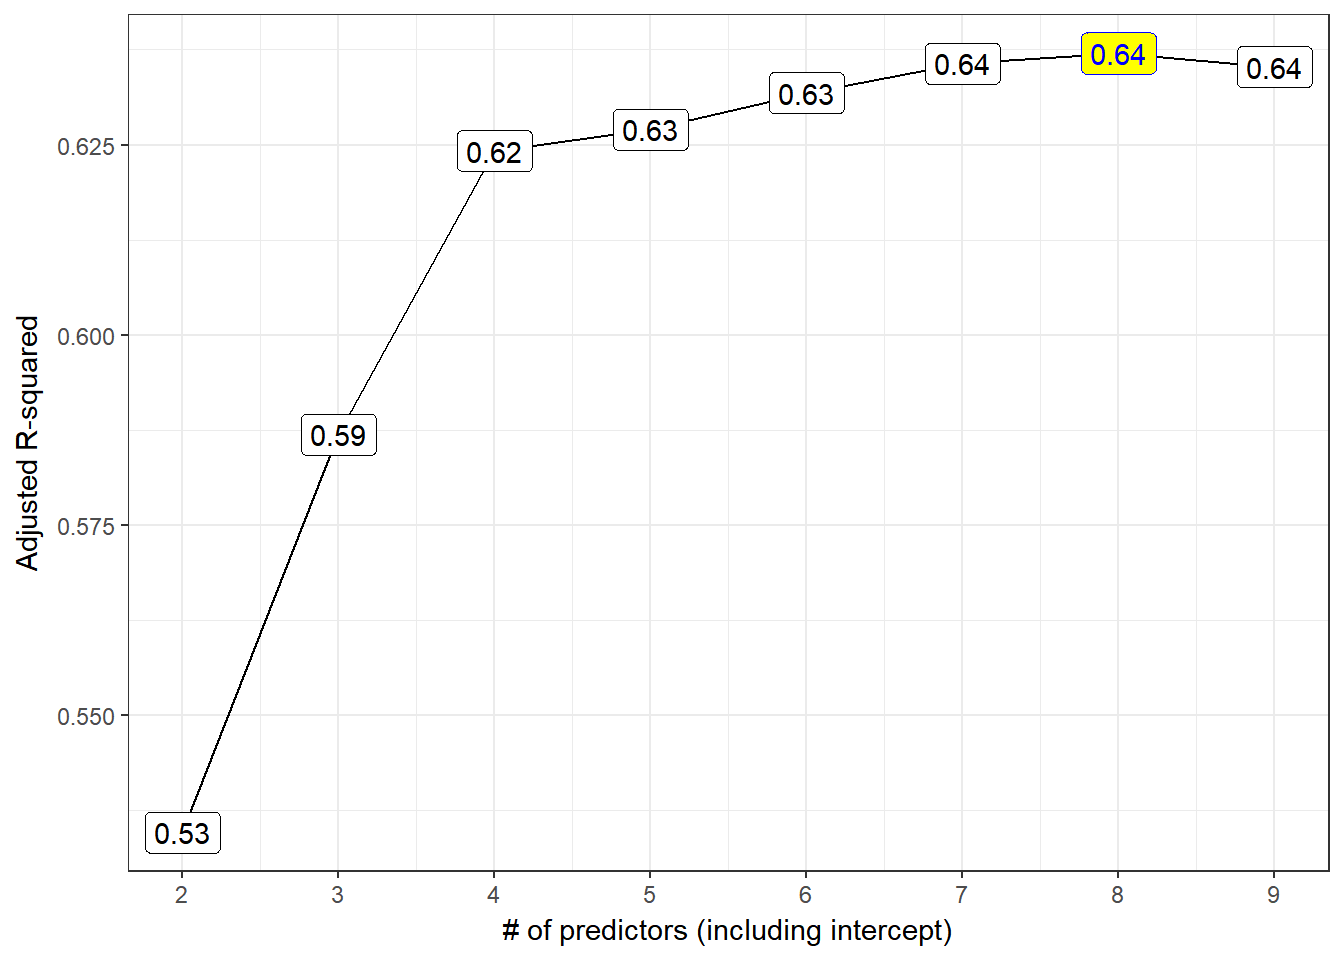
\includegraphics{bookdown-demo_files/figure-latex/unnamed-chunk-77-1.pdf}

Models 4-9 all look like reasonable choices here. The maximum adjusted
R\textsuperscript{2} is seen in the model of size 8.

\subsection{\texorpdfstring{Mallows'
\(C_p\)}{Mallows' C\_p}}\label{mallows-c_p}

The \(C_p\) statistic focuses directly on the tradeoff between
\textbf{bias} (due to excluding important predictors from the model) and
extra \textbf{variance} (due to including too many unimportant
predictors in the model.)

If N is the sample size, and we select \(p\) regression predictors from
a set of \(K\) (where \(p < K\)), then the \(C_p\) statistic is

\(C_p = \frac{SSE_p}{MSE_K} - N + 2p\)

where:

\begin{itemize}
\tightlist
\item
  \(SSE_p\) is the sum of squares for error (residual) in the model with
  \(p\) predictors
\item
  \(MSE_K\) is the residual mean square after regression in the model
  with all \(K\) predictors
\end{itemize}

As it turns out, this is just measuring the particular model's lack of
fit, and then adding a penalty for the number of terms in the model
(specifically \(2p - N\) is the penalty since the lack of fit is
measured as \((N-p) \frac{SSE_p}{MSE_K}\).

\begin{itemize}
\tightlist
\item
  If a model has no meaningful lack of fit (i.e.~no substantial bias)
  then the expected value of \(C_p\) is roughly \(p\).
\item
  Otherwise, the expectation is \(p\) plus a positive bias term.
\item
  In general, we want to see \emph{smaller} values of \(C_p\).
\item
  We usually select a ``winning model'' by choosing a subset of
  predictors that have \(C_p\) near the value of \(p\).
\end{itemize}

\subsection{\texorpdfstring{The \(C_p\)
Plot}{The C\_p Plot}}\label{the-c_p-plot}

The \(C_p\) plot is just a scatterplot of \(C_p\) on the Y-axis, and
\(p\) on the X-axis.

Each of the various predictor subsets we will study is represented in a
single point. A model without bias should have \(C_p\) roughly equal to
\(p\), so we'll frequently draw a line at \(C_p = p\) to make that
clear. We then select our model from among all models with small \(C_p\)
statistics.

\begin{Shaded}
\begin{Highlighting}[]
\NormalTok{p2 <-}\StringTok{ }\KeywordTok{ggplot}\NormalTok{(best_mods, }\KeywordTok{aes}\NormalTok{(}\DataTypeTok{x =}\NormalTok{ k, }\DataTypeTok{y =}\NormalTok{ cp,}
                            \DataTypeTok{label =} \KeywordTok{round}\NormalTok{(cp,}\DecValTok{1}\NormalTok{))) }\OperatorTok{+}
\StringTok{    }\KeywordTok{geom_line}\NormalTok{() }\OperatorTok{+}
\StringTok{    }\KeywordTok{geom_label}\NormalTok{() }\OperatorTok{+}
\StringTok{    }\KeywordTok{geom_abline}\NormalTok{(}\DataTypeTok{intercept =} \DecValTok{0}\NormalTok{, }\DataTypeTok{slope =} \DecValTok{1}\NormalTok{,}
                \DataTypeTok{col =} \StringTok{"red"}\NormalTok{) }\OperatorTok{+}
\StringTok{    }\KeywordTok{theme_bw}\NormalTok{() }\OperatorTok{+}
\StringTok{    }\KeywordTok{scale_x_continuous}\NormalTok{(}\DataTypeTok{breaks =} \DecValTok{2}\OperatorTok{:}\DecValTok{9}\NormalTok{) }\OperatorTok{+}
\StringTok{    }\KeywordTok{labs}\NormalTok{(}\DataTypeTok{x =} \StringTok{"# of predictors (including intercept)"}\NormalTok{,}
         \DataTypeTok{y =} \StringTok{"Mallows' Cp"}\NormalTok{)}

\NormalTok{p2}
\end{Highlighting}
\end{Shaded}

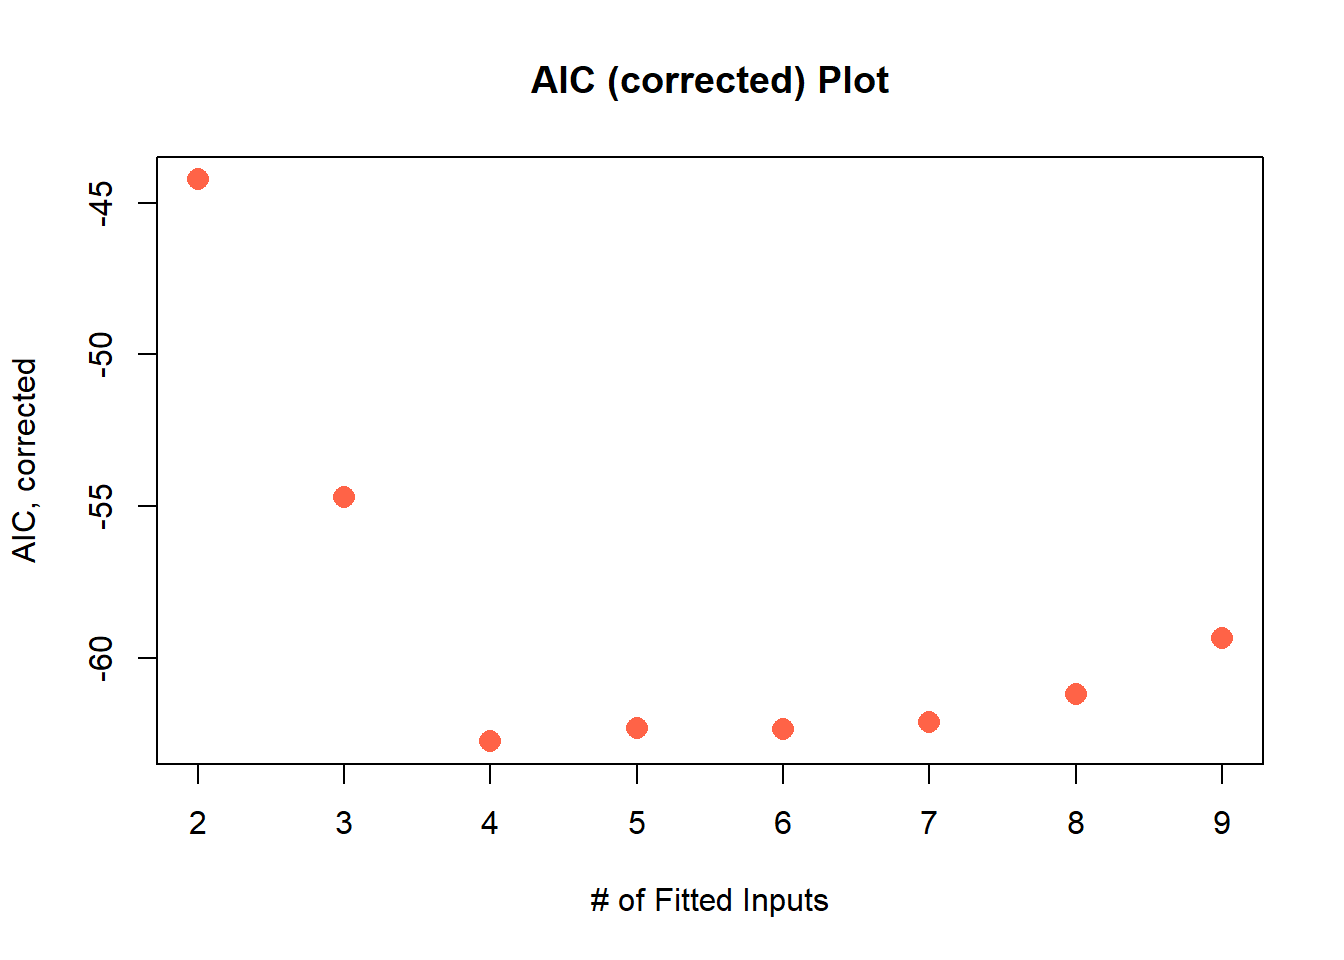
\includegraphics{bookdown-demo_files/figure-latex/unnamed-chunk-78-1.pdf}

\begin{itemize}
\tightlist
\item
  Model 7 looks pretty good, with C\textsubscript{p} just barely smaller
  than the size (p = 7) of the model.
\item
  Model 6 is also a possibility, with the difference \(C_p - p\)
  minimized among all models with \(C_p >= p\).
\end{itemize}

\subsection{\texorpdfstring{``All Subsets'' Regression and Information
Criteria}{All Subsets Regression and Information Criteria}}\label{all-subsets-regression-and-information-criteria}

We might consider any of three main information criteria:

\begin{itemize}
\tightlist
\item
  the Bayesian Information Criterion, called BIC
\item
  the Akaike Information Criterion (used by R's default stepwise
  approaches,) called AIC
\item
  a corrected version of AIC due to Hurwitz and Tsai, called
  AIC\textsubscript{c}
\end{itemize}

Each of these indicates better models by getting smaller. I'll focus on
bias-corrected AIC and on BIC.

\subsection{The bias-corrected AIC
plot}\label{the-bias-corrected-aic-plot}

\begin{Shaded}
\begin{Highlighting}[]
\NormalTok{p3 <-}\StringTok{ }\KeywordTok{ggplot}\NormalTok{(best_mods, }\KeywordTok{aes}\NormalTok{(}\DataTypeTok{x =}\NormalTok{ k, }\DataTypeTok{y =}\NormalTok{ aic.c,}
                             \DataTypeTok{label =} \KeywordTok{round}\NormalTok{(aic.c,}\DecValTok{1}\NormalTok{))) }\OperatorTok{+}
\StringTok{    }\KeywordTok{geom_line}\NormalTok{() }\OperatorTok{+}
\StringTok{    }\KeywordTok{geom_label}\NormalTok{() }\OperatorTok{+}
\StringTok{    }\KeywordTok{geom_label}\NormalTok{(}\DataTypeTok{data =} \KeywordTok{subset}\NormalTok{(best_mods, aic.c }\OperatorTok{==}\StringTok{ }\KeywordTok{min}\NormalTok{(aic.c)),}
               \KeywordTok{aes}\NormalTok{(}\DataTypeTok{x =}\NormalTok{ k, }\DataTypeTok{y =}\NormalTok{ aic.c), }\DataTypeTok{fill =} \StringTok{"pink"}\NormalTok{, }
               \DataTypeTok{col =} \StringTok{"red"}\NormalTok{) }\OperatorTok{+}
\StringTok{    }\KeywordTok{theme_bw}\NormalTok{() }\OperatorTok{+}
\StringTok{    }\KeywordTok{scale_x_continuous}\NormalTok{(}\DataTypeTok{breaks =} \DecValTok{2}\OperatorTok{:}\DecValTok{9}\NormalTok{) }\OperatorTok{+}
\StringTok{    }\KeywordTok{labs}\NormalTok{(}\DataTypeTok{x =} \StringTok{"# of predictors (including intercept)"}\NormalTok{,}
         \DataTypeTok{y =} \StringTok{"Bias-Corrected AIC"}\NormalTok{)}

\NormalTok{p3}
\end{Highlighting}
\end{Shaded}

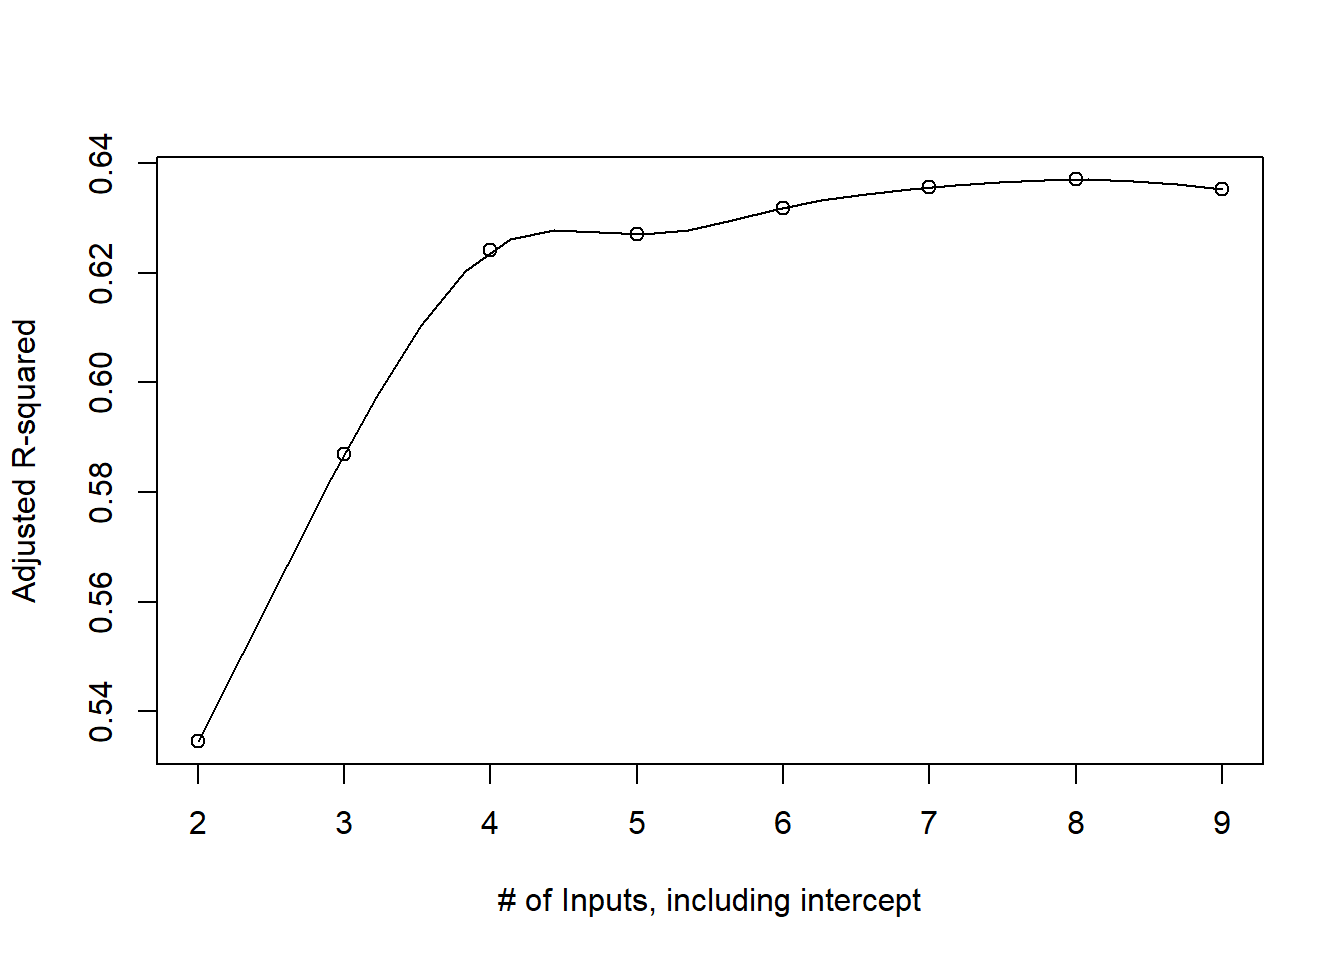
\includegraphics{bookdown-demo_files/figure-latex/unnamed-chunk-79-1.pdf}

The smallest AIC\textsubscript{c} values occur in models 4 and later,
especially model 4 itself.

\subsection{The BIC plot}\label{the-bic-plot}

\begin{Shaded}
\begin{Highlighting}[]
\NormalTok{p4 <-}\StringTok{ }\KeywordTok{ggplot}\NormalTok{(best_mods, }\KeywordTok{aes}\NormalTok{(}\DataTypeTok{x =}\NormalTok{ k, }\DataTypeTok{y =}\NormalTok{ bic,}
                            \DataTypeTok{label =} \KeywordTok{round}\NormalTok{(bic,}\DecValTok{1}\NormalTok{))) }\OperatorTok{+}
\StringTok{    }\KeywordTok{geom_line}\NormalTok{() }\OperatorTok{+}
\StringTok{    }\KeywordTok{geom_label}\NormalTok{() }\OperatorTok{+}
\StringTok{    }\KeywordTok{geom_label}\NormalTok{(}\DataTypeTok{data =} \KeywordTok{subset}\NormalTok{(best_mods, bic }\OperatorTok{==}\StringTok{ }\KeywordTok{min}\NormalTok{(bic)),}
               \KeywordTok{aes}\NormalTok{(}\DataTypeTok{x =}\NormalTok{ k, }\DataTypeTok{y =}\NormalTok{ bic),}
               \DataTypeTok{fill =} \StringTok{"lightgreen"}\NormalTok{, }\DataTypeTok{col =} \StringTok{"blue"}\NormalTok{) }\OperatorTok{+}
\StringTok{    }\KeywordTok{theme_bw}\NormalTok{() }\OperatorTok{+}
\StringTok{    }\KeywordTok{scale_x_continuous}\NormalTok{(}\DataTypeTok{breaks =} \DecValTok{2}\OperatorTok{:}\DecValTok{9}\NormalTok{) }\OperatorTok{+}
\StringTok{    }\KeywordTok{labs}\NormalTok{(}\DataTypeTok{x =} \StringTok{"# of predictors (including intercept)"}\NormalTok{,}
         \DataTypeTok{y =} \StringTok{"BIC"}\NormalTok{)}

\NormalTok{p4}
\end{Highlighting}
\end{Shaded}

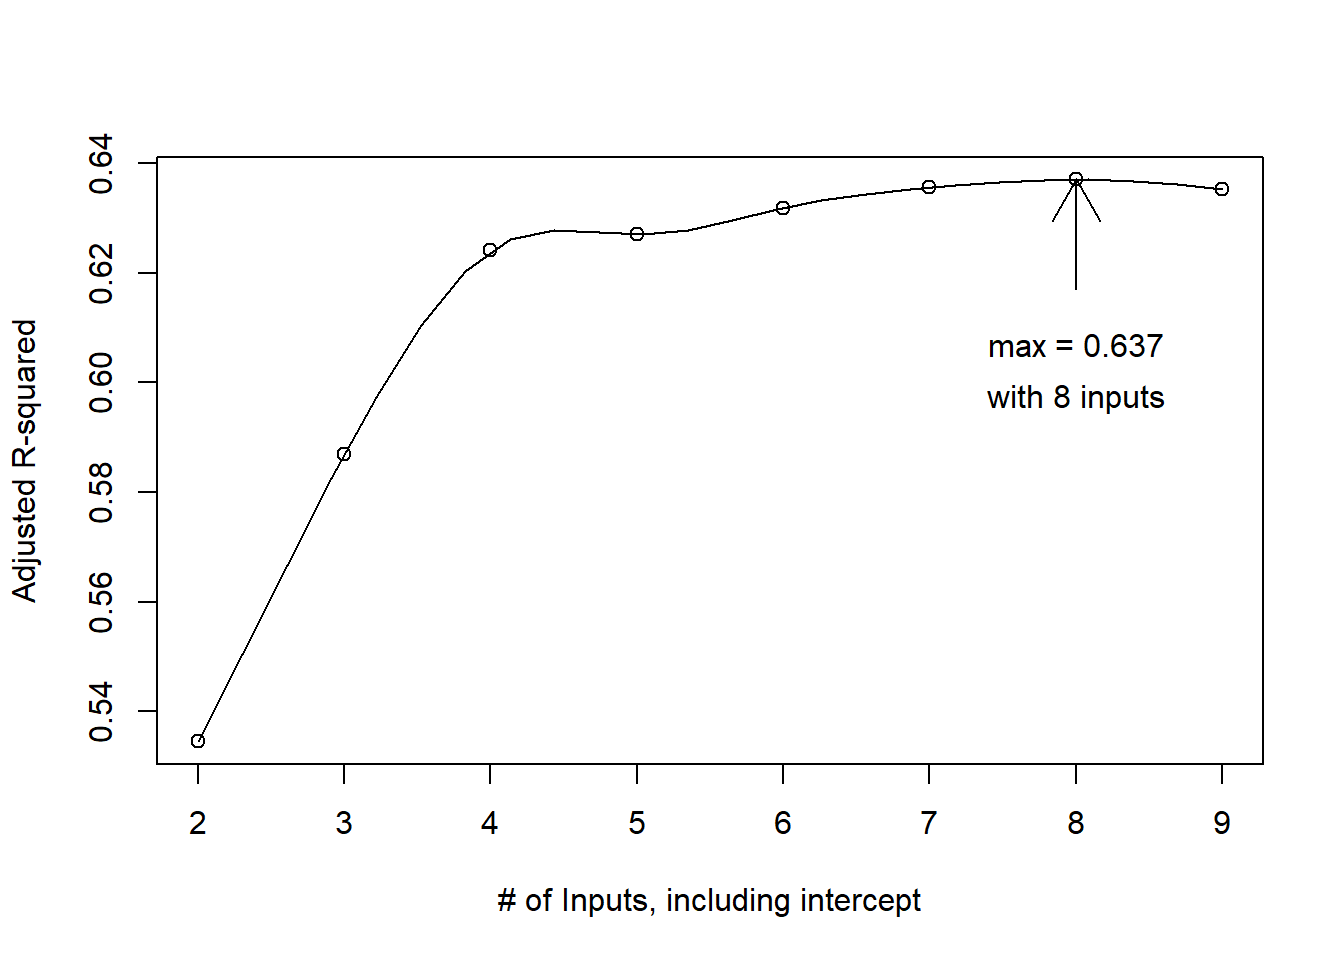
\includegraphics{bookdown-demo_files/figure-latex/unnamed-chunk-80-1.pdf}

\subsection{All Four Plots in One Figure (via
ggplot2)}\label{all-four-plots-in-one-figure-via-ggplot2}

\begin{Shaded}
\begin{Highlighting}[]
\NormalTok{gridExtra}\OperatorTok{::}\KeywordTok{grid.arrange}\NormalTok{(p1, p2, p3, p4, }\DataTypeTok{nrow =} \DecValTok{2}\NormalTok{)}
\end{Highlighting}
\end{Shaded}

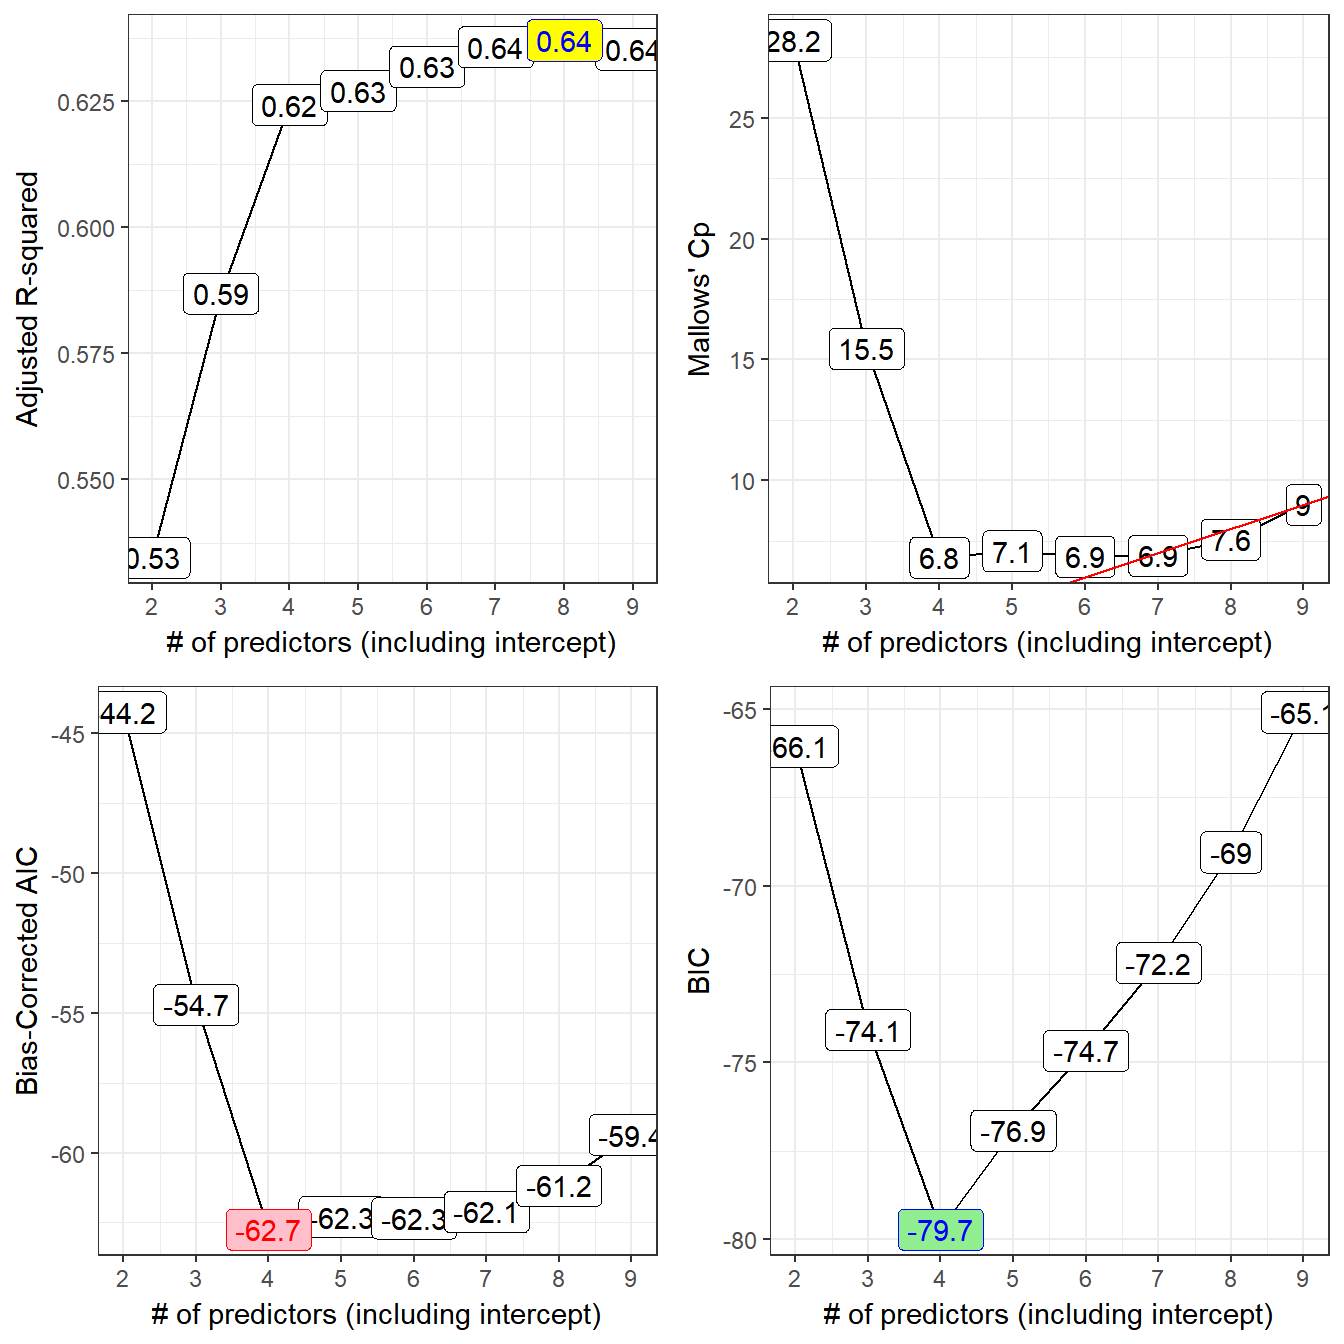
\includegraphics{bookdown-demo_files/figure-latex/unnamed-chunk-81-1.pdf}

\section{Plotting the Best Subsets Results using base R
plots}\label{plotting-the-best-subsets-results-using-base-r-plots}

\subsection{\texorpdfstring{The Adjusted R\textsuperscript{2}
Plot}{The Adjusted R2 Plot}}\label{the-adjusted-r2-plot-1}

\begin{Shaded}
\begin{Highlighting}[]
\KeywordTok{plot}\NormalTok{(rs}\OperatorTok{$}\NormalTok{adjr2 }\OperatorTok{~}\StringTok{ }\KeywordTok{I}\NormalTok{(}\DecValTok{2}\OperatorTok{:}\DecValTok{9}\NormalTok{), }\DataTypeTok{ylab=}\StringTok{"Adjusted R-squared"}\NormalTok{,}
     \DataTypeTok{xlab=}\StringTok{"# of Inputs, including intercept"}\NormalTok{)}
\KeywordTok{lines}\NormalTok{(}\KeywordTok{spline}\NormalTok{(rs}\OperatorTok{$}\NormalTok{adjr2 }\OperatorTok{~}\StringTok{ }\KeywordTok{I}\NormalTok{(}\DecValTok{2}\OperatorTok{:}\DecValTok{9}\NormalTok{)))}
\end{Highlighting}
\end{Shaded}

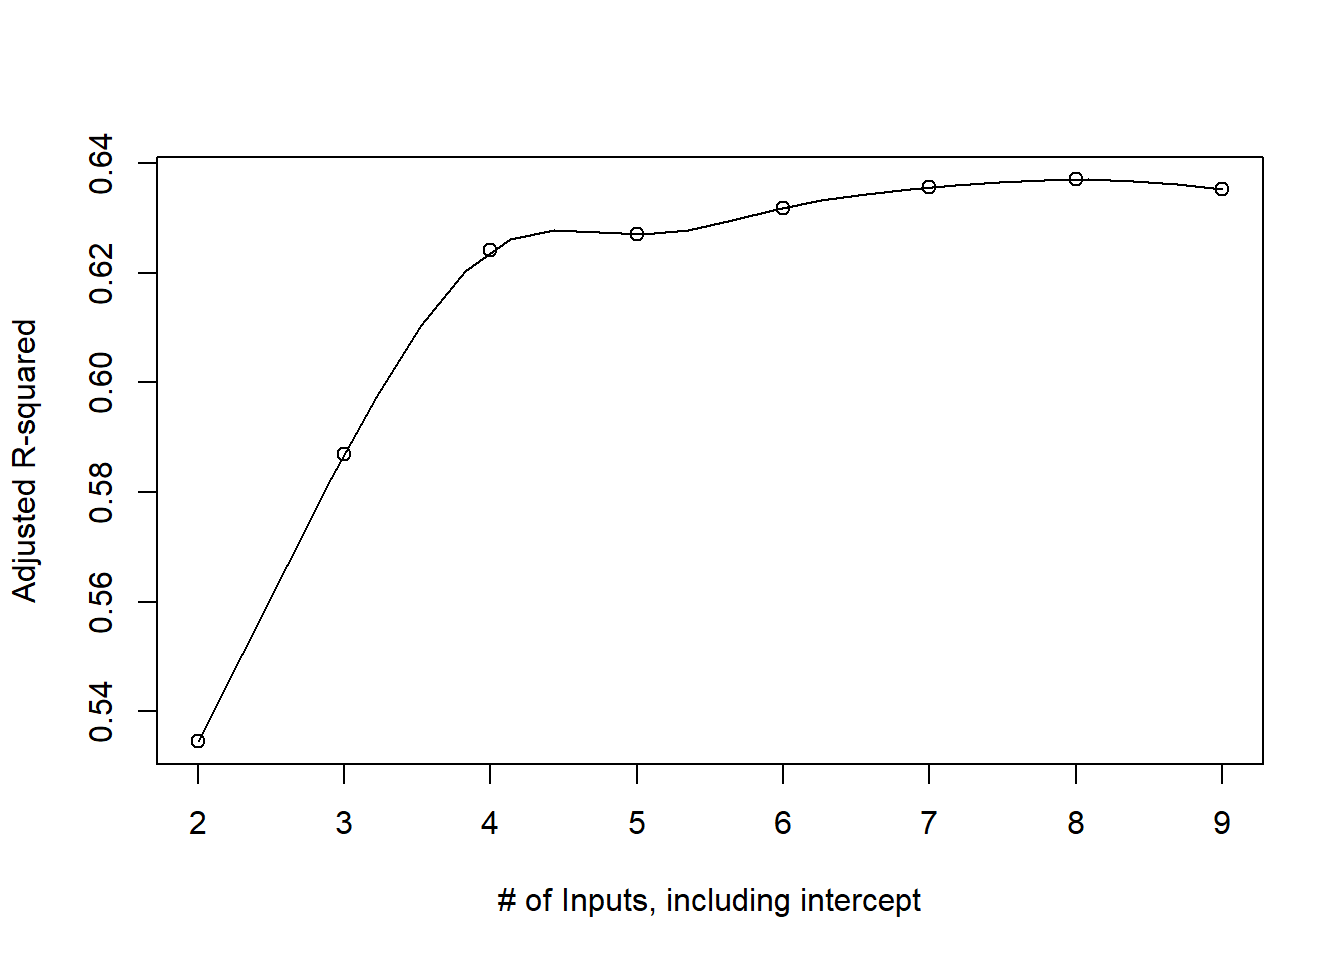
\includegraphics{bookdown-demo_files/figure-latex/unnamed-chunk-82-1.pdf}

Again, models 4-9 all look like reasonable choices here.

\subsection{\texorpdfstring{A Fancier Version (identifying the largest
adjusted
R\textsuperscript{2})}{A Fancier Version (identifying the largest adjusted R2)}}\label{a-fancier-version-identifying-the-largest-adjusted-r2}

\begin{Shaded}
\begin{Highlighting}[]
\NormalTok{m2 <-}\StringTok{ }\KeywordTok{max}\NormalTok{(rs}\OperatorTok{$}\NormalTok{adjr2) }
\NormalTok{m1 <-}\StringTok{ }\KeywordTok{which.max}\NormalTok{(rs}\OperatorTok{$}\NormalTok{adjr2) }\OperatorTok{+}\StringTok{ }\DecValTok{1}
\KeywordTok{plot}\NormalTok{(rs}\OperatorTok{$}\NormalTok{adjr2 }\OperatorTok{~}\StringTok{ }\KeywordTok{I}\NormalTok{(}\DecValTok{2}\OperatorTok{:}\DecValTok{9}\NormalTok{), }\DataTypeTok{ylab=}\StringTok{"Adjusted R-squared"}\NormalTok{,}
     \DataTypeTok{xlab=}\StringTok{"# of Inputs, including intercept"}\NormalTok{)}
\KeywordTok{lines}\NormalTok{(}\KeywordTok{spline}\NormalTok{(rs}\OperatorTok{$}\NormalTok{adjr2 }\OperatorTok{~}\StringTok{ }\KeywordTok{I}\NormalTok{(}\DecValTok{2}\OperatorTok{:}\DecValTok{9}\NormalTok{)))}
\KeywordTok{arrows}\NormalTok{(m1, m2}\OperatorTok{-}\FloatTok{0.02}\NormalTok{, m1, m2)}
\KeywordTok{text}\NormalTok{(m1, m2}\OperatorTok{-}\FloatTok{0.03}\NormalTok{, }\KeywordTok{paste}\NormalTok{(}\StringTok{"max ="}\NormalTok{, }\KeywordTok{format}\NormalTok{(m2, }\DataTypeTok{digits=}\DecValTok{3}\NormalTok{)))}
\KeywordTok{text}\NormalTok{(m1, m2}\OperatorTok{-}\FloatTok{0.045}\NormalTok{, }\KeywordTok{paste}\NormalTok{(}\StringTok{"with"}\NormalTok{, }\KeywordTok{format}\NormalTok{(m1, }\DataTypeTok{digits=}\DecValTok{1}\NormalTok{),}
                        \StringTok{"inputs"}\NormalTok{), }\DataTypeTok{pos=}\DecValTok{3}\NormalTok{)}
\end{Highlighting}
\end{Shaded}

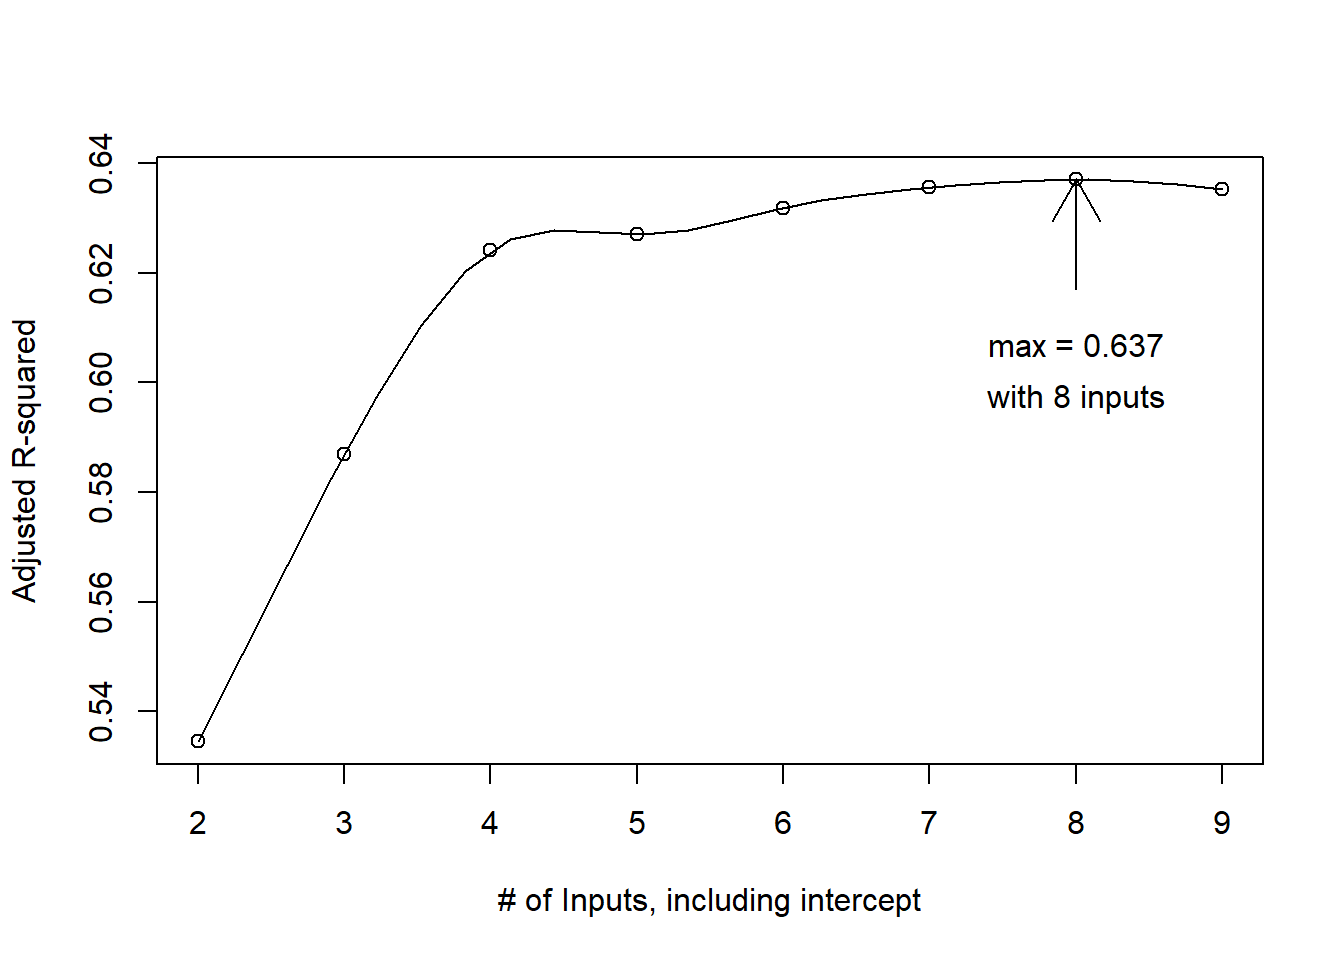
\includegraphics{bookdown-demo_files/figure-latex/unnamed-chunk-83-1.pdf}

\subsection{\texorpdfstring{The \(C_p\)
Plot}{The C\_p Plot}}\label{the-c_p-plot-1}

Again, the \(C_p\) plot is just a scatterplot of \(C_p\) on the Y-axis,
and \(p\) on the X-axis.

Each of the various predictor subsets we will study is represented in a
single point. A model without bias should have \(C_p\) roughly equal to
\(p\), so we'll frequently draw a line at \(C_p = p\) to make that
clear. We then select our model from among all models with small \(C_p\)
statistics.

\begin{Shaded}
\begin{Highlighting}[]
\KeywordTok{plot}\NormalTok{(rs}\OperatorTok{$}\NormalTok{cp }\OperatorTok{~}\StringTok{ }\KeywordTok{I}\NormalTok{(}\DecValTok{2}\OperatorTok{:}\DecValTok{9}\NormalTok{),}
     \DataTypeTok{ylab=}\StringTok{"Cp Statistic"}\NormalTok{,}
     \DataTypeTok{xlab=}\StringTok{"# of Regression Inputs, including Intercept"}\NormalTok{,}
     \DataTypeTok{pch=}\DecValTok{16}\NormalTok{, }\DataTypeTok{main=}\StringTok{"Cp Plot"}\NormalTok{)}
\KeywordTok{abline}\NormalTok{(}\DecValTok{0}\NormalTok{,}\DecValTok{1}\NormalTok{, }\DataTypeTok{col =} \StringTok{"purple"}\NormalTok{)}
\end{Highlighting}
\end{Shaded}

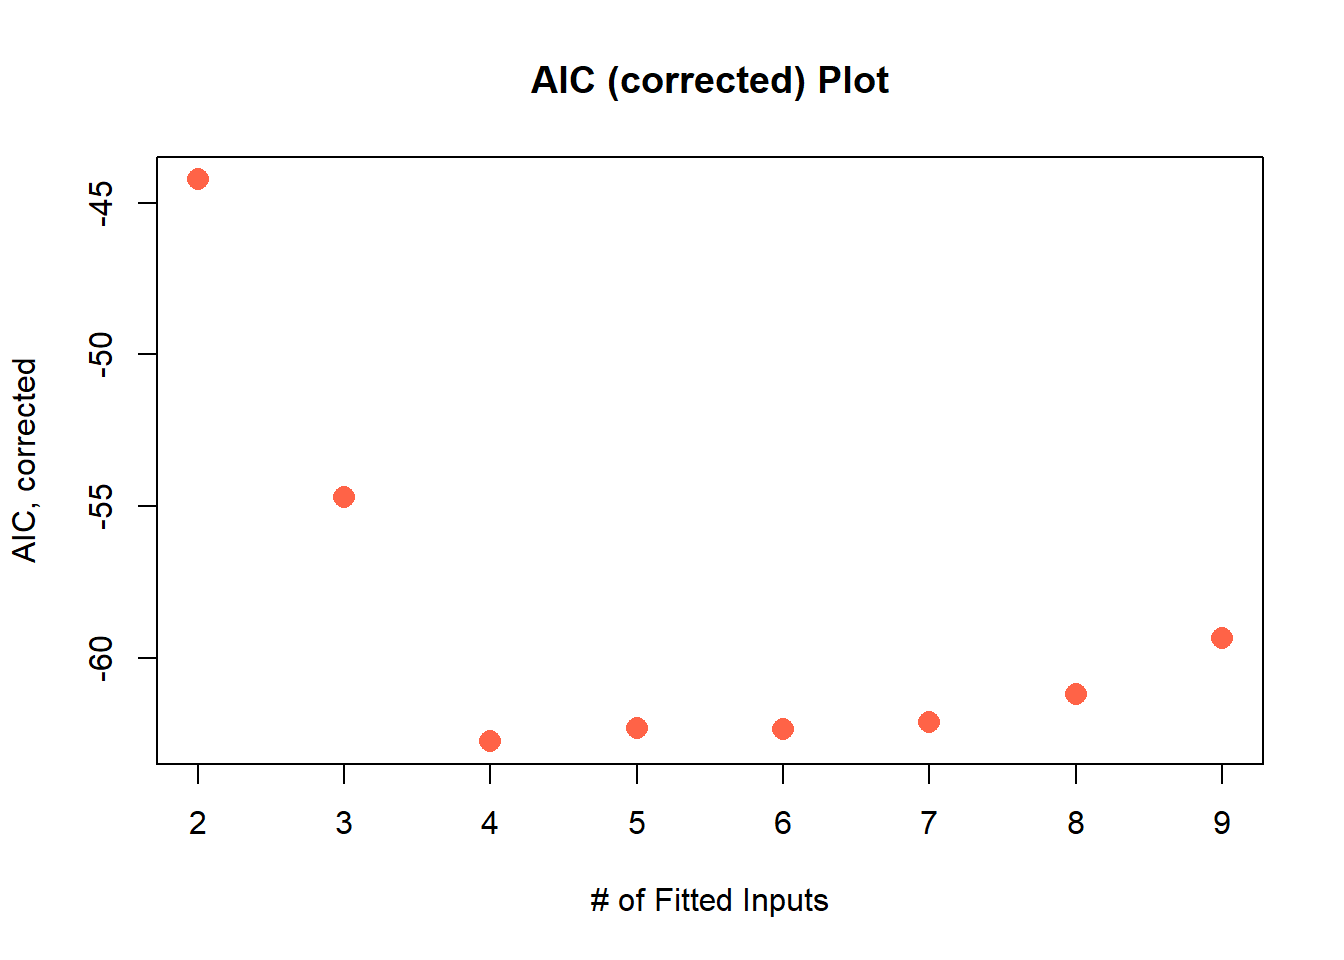
\includegraphics{bookdown-demo_files/figure-latex/unnamed-chunk-84-1.pdf}

Model 4 has the smallest value of \(C_p\) (and is the leftmost of the
largely comparable models 4-9) while 6 is close to and 7 is right on the
\(C_p = p\) line, so those are the likeliest candidates.

\subsection{The BIC Plot}\label{the-bic-plot-1}

R provides the BIC directly as part of the result of running
\texttt{regsubsets}, as we've seen.

\begin{Shaded}
\begin{Highlighting}[]
\KeywordTok{plot}\NormalTok{(rs}\OperatorTok{$}\NormalTok{bic }\OperatorTok{~}\StringTok{ }\KeywordTok{I}\NormalTok{(}\DecValTok{2}\OperatorTok{:}\DecValTok{9}\NormalTok{), }\DataTypeTok{ylab=}\StringTok{"BIC"}\NormalTok{, }\DataTypeTok{xlab=}\StringTok{"# of Fitted Inputs"}\NormalTok{,}
     \DataTypeTok{pch=}\DecValTok{16}\NormalTok{, }\DataTypeTok{cex=}\FloatTok{1.5}\NormalTok{, }\DataTypeTok{col=}\StringTok{"slateblue"}\NormalTok{, }\DataTypeTok{main=}\StringTok{"BIC Plot"}\NormalTok{)}
\end{Highlighting}
\end{Shaded}

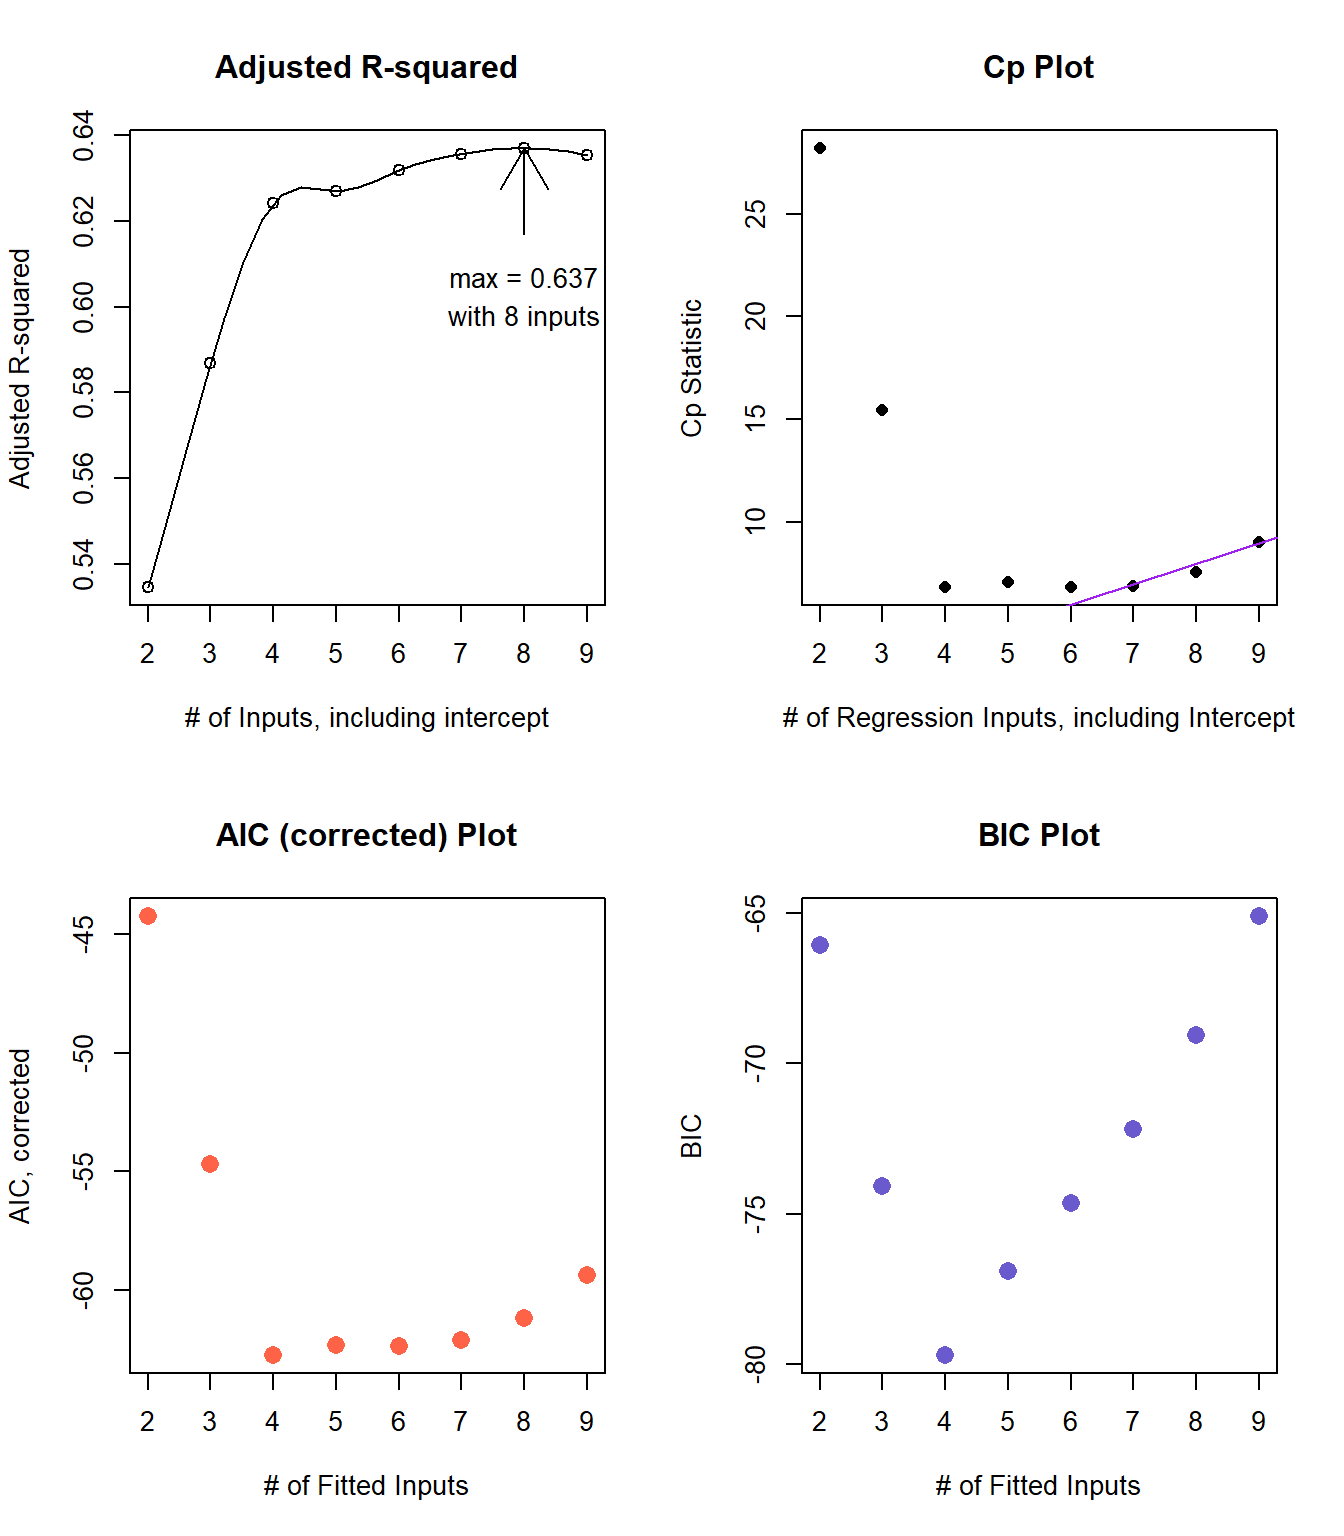
\includegraphics{bookdown-demo_files/figure-latex/unnamed-chunk-85-1.pdf}

We want to minimize BIC, which argues strongly for the model with 4
inputs, including the intercept.

\subsection{The Bias-Corrected AIC (Hurwitz \&
Tsai)}\label{the-bias-corrected-aic-hurwitz-tsai}

The bias-corrected AIC formula due to Hurwitz and Tsai is, as we've
seen:

\[
AIC_c = n log(\frac{RSS}{n}) + 2k + \frac{2k (k+1)}{n-k-1}
\]

\begin{Shaded}
\begin{Highlighting}[]
\NormalTok{rs}\OperatorTok{$}\NormalTok{aic.c <-}\StringTok{ }\DecValTok{97}\OperatorTok{*}\KeywordTok{log}\NormalTok{(rs}\OperatorTok{$}\NormalTok{rss }\OperatorTok{/}\StringTok{ }\DecValTok{97}\NormalTok{) }\OperatorTok{+}\StringTok{ }\DecValTok{2}\OperatorTok{*}\NormalTok{(}\DecValTok{2}\OperatorTok{:}\DecValTok{9}\NormalTok{) }\OperatorTok{+}
\StringTok{               }\NormalTok{(}\DecValTok{2} \OperatorTok{*}\StringTok{ }\NormalTok{(}\DecValTok{2}\OperatorTok{:}\DecValTok{9}\NormalTok{) }\OperatorTok{*}\StringTok{ }\NormalTok{((}\DecValTok{2}\OperatorTok{:}\DecValTok{9}\NormalTok{)}\OperatorTok{+}\DecValTok{1}\NormalTok{) }\OperatorTok{/}\StringTok{ }\NormalTok{(}\DecValTok{97} \OperatorTok{-}\StringTok{ }\NormalTok{(}\DecValTok{2}\OperatorTok{:}\DecValTok{9}\NormalTok{) }\OperatorTok{-}\StringTok{ }\DecValTok{1}\NormalTok{))}

\KeywordTok{round}\NormalTok{(rs}\OperatorTok{$}\NormalTok{aic,}\DecValTok{2}\NormalTok{) }\CommentTok{# uncorrected }
\end{Highlighting}
\end{Shaded}

\begin{verbatim}
[1] -44.24 -54.70 -62.74 -62.29 -62.34 -62.11 -61.17 -59.36
\end{verbatim}

\begin{Shaded}
\begin{Highlighting}[]
\KeywordTok{round}\NormalTok{(rs}\OperatorTok{$}\NormalTok{aic.c,}\DecValTok{2}\NormalTok{) }\CommentTok{# bias-corrected}
\end{Highlighting}
\end{Shaded}

\begin{verbatim}
[1] -44.24 -54.70 -62.74 -62.29 -62.34 -62.11 -61.17 -59.36
\end{verbatim}

\begin{Shaded}
\begin{Highlighting}[]
\KeywordTok{plot}\NormalTok{(rs}\OperatorTok{$}\NormalTok{aic.c }\OperatorTok{~}\StringTok{ }\KeywordTok{I}\NormalTok{(}\DecValTok{2}\OperatorTok{:}\DecValTok{9}\NormalTok{), }\DataTypeTok{ylab=}\StringTok{"AIC, corrected"}\NormalTok{, }\DataTypeTok{xlab=}\StringTok{"# of Fitted Inputs"}\NormalTok{,}
     \DataTypeTok{pch=}\DecValTok{16}\NormalTok{, }\DataTypeTok{cex=}\FloatTok{1.5}\NormalTok{, }\DataTypeTok{col=}\StringTok{"tomato"}\NormalTok{, }\DataTypeTok{main=}\StringTok{"AIC (corrected) Plot"}\NormalTok{)}
\end{Highlighting}
\end{Shaded}

\includegraphics{bookdown-demo_files/figure-latex/unnamed-chunk-87-1.pdf}

The smallest AIC\textsubscript{c} values occur in models 4 and later,
especially model 4 itself.

\subsection{All Four Plots, Together (from Base
R)}\label{all-four-plots-together-from-base-r}

\begin{Shaded}
\begin{Highlighting}[]
\KeywordTok{par}\NormalTok{(}\DataTypeTok{mfrow =} \KeywordTok{c}\NormalTok{(}\DecValTok{2}\NormalTok{,}\DecValTok{2}\NormalTok{))}
\NormalTok{m2 <-}\StringTok{ }\KeywordTok{max}\NormalTok{(rs}\OperatorTok{$}\NormalTok{adjr2) }
\NormalTok{m1 <-}\StringTok{ }\KeywordTok{which.max}\NormalTok{(rs}\OperatorTok{$}\NormalTok{adjr2) }\OperatorTok{+}\StringTok{ }\DecValTok{1}
\KeywordTok{plot}\NormalTok{(rs}\OperatorTok{$}\NormalTok{adjr2 }\OperatorTok{~}\StringTok{ }\KeywordTok{I}\NormalTok{(}\DecValTok{2}\OperatorTok{:}\DecValTok{9}\NormalTok{), }\DataTypeTok{ylab=}\StringTok{"Adjusted R-squared"}\NormalTok{,}
     \DataTypeTok{xlab=}\StringTok{"# of Inputs, including intercept"}\NormalTok{,}
     \DataTypeTok{main =} \StringTok{"Adjusted R-squared"}\NormalTok{)}
\KeywordTok{lines}\NormalTok{(}\KeywordTok{spline}\NormalTok{(rs}\OperatorTok{$}\NormalTok{adjr2 }\OperatorTok{~}\StringTok{ }\KeywordTok{I}\NormalTok{(}\DecValTok{2}\OperatorTok{:}\DecValTok{9}\NormalTok{)))}
\KeywordTok{arrows}\NormalTok{(m1, m2}\OperatorTok{-}\FloatTok{0.02}\NormalTok{, m1, m2)}
\KeywordTok{text}\NormalTok{(m1, m2}\OperatorTok{-}\FloatTok{0.03}\NormalTok{, }\KeywordTok{paste}\NormalTok{(}\StringTok{"max ="}\NormalTok{, }\KeywordTok{format}\NormalTok{(m2, }\DataTypeTok{digits=}\DecValTok{3}\NormalTok{)))}
\KeywordTok{text}\NormalTok{(m1, m2}\OperatorTok{-}\FloatTok{0.045}\NormalTok{, }\KeywordTok{paste}\NormalTok{(}\StringTok{"with"}\NormalTok{, }\KeywordTok{format}\NormalTok{(m1, }\DataTypeTok{digits=}\DecValTok{1}\NormalTok{),}
                        \StringTok{"inputs"}\NormalTok{), }\DataTypeTok{pos=}\DecValTok{3}\NormalTok{)}

\KeywordTok{plot}\NormalTok{(rs}\OperatorTok{$}\NormalTok{cp }\OperatorTok{~}\StringTok{ }\KeywordTok{I}\NormalTok{(}\DecValTok{2}\OperatorTok{:}\DecValTok{9}\NormalTok{),}
     \DataTypeTok{ylab=}\StringTok{"Cp Statistic"}\NormalTok{,}
     \DataTypeTok{xlab=}\StringTok{"# of Regression Inputs, including Intercept"}\NormalTok{,}
     \DataTypeTok{pch=}\DecValTok{16}\NormalTok{, }\DataTypeTok{main=}\StringTok{"Cp Plot"}\NormalTok{)}
\KeywordTok{abline}\NormalTok{(}\DecValTok{0}\NormalTok{,}\DecValTok{1}\NormalTok{, }\DataTypeTok{col =} \StringTok{"purple"}\NormalTok{)}

\NormalTok{rs}\OperatorTok{$}\NormalTok{aic.c <-}\StringTok{ }\DecValTok{97}\OperatorTok{*}\KeywordTok{log}\NormalTok{(rs}\OperatorTok{$}\NormalTok{rss }\OperatorTok{/}\StringTok{ }\DecValTok{97}\NormalTok{) }\OperatorTok{+}\StringTok{ }\DecValTok{2}\OperatorTok{*}\NormalTok{(}\DecValTok{2}\OperatorTok{:}\DecValTok{9}\NormalTok{) }\OperatorTok{+}
\StringTok{               }\NormalTok{(}\DecValTok{2} \OperatorTok{*}\StringTok{ }\NormalTok{(}\DecValTok{2}\OperatorTok{:}\DecValTok{9}\NormalTok{) }\OperatorTok{*}\StringTok{ }\NormalTok{((}\DecValTok{2}\OperatorTok{:}\DecValTok{9}\NormalTok{)}\OperatorTok{+}\DecValTok{1}\NormalTok{) }\OperatorTok{/}\StringTok{ }\NormalTok{(}\DecValTok{97} \OperatorTok{-}\StringTok{ }\NormalTok{(}\DecValTok{2}\OperatorTok{:}\DecValTok{9}\NormalTok{) }\OperatorTok{-}\StringTok{ }\DecValTok{1}\NormalTok{))}
\KeywordTok{plot}\NormalTok{(rs}\OperatorTok{$}\NormalTok{aic.c }\OperatorTok{~}\StringTok{ }\KeywordTok{I}\NormalTok{(}\DecValTok{2}\OperatorTok{:}\DecValTok{9}\NormalTok{), }\DataTypeTok{ylab=}\StringTok{"AIC, corrected"}\NormalTok{, }\DataTypeTok{xlab=}\StringTok{"# of Fitted Inputs"}\NormalTok{,}
     \DataTypeTok{pch=}\DecValTok{16}\NormalTok{, }\DataTypeTok{cex=}\FloatTok{1.5}\NormalTok{, }\DataTypeTok{col=}\StringTok{"tomato"}\NormalTok{, }\DataTypeTok{main=}\StringTok{"AIC (corrected) Plot"}\NormalTok{)}

\KeywordTok{plot}\NormalTok{(rs}\OperatorTok{$}\NormalTok{bic }\OperatorTok{~}\StringTok{ }\KeywordTok{I}\NormalTok{(}\DecValTok{2}\OperatorTok{:}\DecValTok{9}\NormalTok{), }\DataTypeTok{ylab=}\StringTok{"BIC"}\NormalTok{, }\DataTypeTok{xlab=}\StringTok{"# of Fitted Inputs"}\NormalTok{,}
     \DataTypeTok{pch=}\DecValTok{16}\NormalTok{, }\DataTypeTok{cex=}\FloatTok{1.5}\NormalTok{, }\DataTypeTok{col=}\StringTok{"slateblue"}\NormalTok{, }\DataTypeTok{main=}\StringTok{"BIC Plot"}\NormalTok{)}
\end{Highlighting}
\end{Shaded}

\includegraphics{bookdown-demo_files/figure-latex/unnamed-chunk-88-1.pdf}

\begin{Shaded}
\begin{Highlighting}[]
\KeywordTok{par}\NormalTok{(}\DataTypeTok{mfrow =} \KeywordTok{c}\NormalTok{(}\DecValTok{1}\NormalTok{,}\DecValTok{1}\NormalTok{))}
\end{Highlighting}
\end{Shaded}

\section{Table of Key Results}\label{table-of-key-results}

We can build a big table, like this:

\begin{Shaded}
\begin{Highlighting}[]
\NormalTok{best_mods}
\end{Highlighting}
\end{Shaded}

\begin{verbatim}
  k        r2     adjr2        cp     aic.c       bic (Intercept) lcavol
1 2 0.5394320 0.5345839 28.213914 -44.23838 -66.05416        TRUE   TRUE
2 3 0.5955040 0.5868977 15.456669 -54.70040 -74.07188        TRUE   TRUE
3 4 0.6359499 0.6242063  6.811986 -62.74265 -79.71614        TRUE   TRUE
4 5 0.6425479 0.6270065  7.075509 -62.29223 -76.91557        TRUE   TRUE
5 6 0.6509970 0.6318211  6.851826 -62.33858 -74.66120        TRUE   TRUE
6 7 0.6584484 0.6356783  6.890739 -62.10692 -72.17992        TRUE   TRUE
7 8 0.6634967 0.6370302  7.562119 -61.17338 -69.04961        TRUE   TRUE
8 9 0.6656326 0.6352355  9.000000 -59.35841 -65.09253        TRUE   TRUE
  lweight   age bph_f svi_f   lcp gleason_f pgg45
1   FALSE FALSE FALSE FALSE FALSE     FALSE FALSE
2    TRUE FALSE FALSE FALSE FALSE     FALSE FALSE
3    TRUE FALSE FALSE  TRUE FALSE     FALSE FALSE
4    TRUE FALSE  TRUE  TRUE FALSE     FALSE FALSE
5    TRUE  TRUE  TRUE  TRUE FALSE     FALSE FALSE
6    TRUE  TRUE  TRUE  TRUE FALSE      TRUE FALSE
7    TRUE  TRUE  TRUE  TRUE  TRUE      TRUE FALSE
8    TRUE  TRUE  TRUE  TRUE  TRUE      TRUE  TRUE
\end{verbatim}

\section{Models Worth Considering?}\label{models-worth-considering}

\begin{longtable}[]{@{}rrll@{}}
\toprule
\(k\) & Predictors & Reason\tabularnewline
\midrule
\endhead
4 & \texttt{lcavol\ lweight\ svi\_f} & minimizes BIC,
AIC\textsubscript{c}\tabularnewline
7 & \texttt{+\ age\ bph\_f\ gleason\_f} & \(C_p\) near
\emph{p}\tabularnewline
8 & \texttt{+\ lcp} & max \(R^2_{adj}\)\tabularnewline
\bottomrule
\end{longtable}

\section{Compare these candidate models
in-sample?}\label{compare-these-candidate-models-in-sample}

\subsection{\texorpdfstring{Using \texttt{anova} to compare nested
models}{Using anova to compare nested models}}\label{using-anova-to-compare-nested-models}

Let's run an ANOVA-based comparison of these nested models to each other
and to the model with the intercept alone.

\begin{itemize}
\tightlist
\item
  The models are \textbf{nested} because \texttt{m04} is a subset of the
  predictors in \texttt{m07}, which includes a subset of the predictors
  in \texttt{m08}.
\end{itemize}

\begin{Shaded}
\begin{Highlighting}[]
\NormalTok{m.int <-}\StringTok{ }\KeywordTok{lm}\NormalTok{(lpsa }\OperatorTok{~}\StringTok{ }\DecValTok{1}\NormalTok{, }\DataTypeTok{data =}\NormalTok{ prost)}
\NormalTok{m04 <-}\StringTok{ }\KeywordTok{lm}\NormalTok{(lpsa }\OperatorTok{~}\StringTok{ }\NormalTok{lcavol }\OperatorTok{+}\StringTok{ }\NormalTok{lweight }\OperatorTok{+}\StringTok{ }\NormalTok{svi_f, }\DataTypeTok{data =}\NormalTok{ prost)}
\NormalTok{m07 <-}\StringTok{ }\KeywordTok{lm}\NormalTok{(lpsa }\OperatorTok{~}\StringTok{ }\NormalTok{lcavol }\OperatorTok{+}\StringTok{ }\NormalTok{lweight }\OperatorTok{+}\StringTok{ }\NormalTok{svi_f }\OperatorTok{+}\StringTok{ }
\StringTok{              }\NormalTok{age }\OperatorTok{+}\StringTok{ }\NormalTok{bph_f }\OperatorTok{+}\StringTok{ }\NormalTok{gleason_f, }\DataTypeTok{data =}\NormalTok{ prost)}
\NormalTok{m08 <-}\StringTok{ }\KeywordTok{lm}\NormalTok{(lpsa }\OperatorTok{~}\StringTok{ }\NormalTok{lcavol }\OperatorTok{+}\StringTok{ }\NormalTok{lweight }\OperatorTok{+}\StringTok{ }\NormalTok{svi_f }\OperatorTok{+}\StringTok{ }
\StringTok{              }\NormalTok{age }\OperatorTok{+}\StringTok{ }\NormalTok{bph_f }\OperatorTok{+}\StringTok{ }\NormalTok{gleason_f }\OperatorTok{+}\StringTok{ }\NormalTok{lcp, }\DataTypeTok{data =}\NormalTok{ prost)}
\NormalTok{m.full <-}\StringTok{ }\KeywordTok{lm}\NormalTok{(lpsa }\OperatorTok{~}\StringTok{ }\NormalTok{lcavol }\OperatorTok{+}\StringTok{ }\NormalTok{lweight }\OperatorTok{+}\StringTok{ }\NormalTok{svi_f }\OperatorTok{+}\StringTok{ }
\StringTok{              }\NormalTok{age }\OperatorTok{+}\StringTok{ }\NormalTok{bph_f }\OperatorTok{+}\StringTok{ }\NormalTok{gleason_f }\OperatorTok{+}\StringTok{ }\NormalTok{lcp }\OperatorTok{+}\StringTok{ }\NormalTok{pgg45, }\DataTypeTok{data =}\NormalTok{ prost)}
\end{Highlighting}
\end{Shaded}

Next, we'll run\ldots{}

\begin{Shaded}
\begin{Highlighting}[]
\KeywordTok{anova}\NormalTok{(m.full, m08, m07, m04, m.int)}
\end{Highlighting}
\end{Shaded}

\begin{verbatim}
Analysis of Variance Table

Model 1: lpsa ~ lcavol + lweight + svi_f + age + bph_f + gleason_f + lcp + 
    pgg45
Model 2: lpsa ~ lcavol + lweight + svi_f + age + bph_f + gleason_f + lcp
Model 3: lpsa ~ lcavol + lweight + svi_f + age + bph_f + gleason_f
Model 4: lpsa ~ lcavol + lweight + svi_f
Model 5: lpsa ~ 1
  Res.Df     RSS Df Sum of Sq       F Pr(>F)    
1     86  41.057                                
2     87  41.498 -1    -0.441  0.9234 0.3393    
3     88  42.066 -1    -0.568  1.1891 0.2786    
4     93  46.568 -5    -4.503  1.8863 0.1050    
5     96 127.918 -3   -81.349 56.7991 <2e-16 ***
---
Signif. codes:  0 '***' 0.001 '**' 0.01 '*' 0.05 '.' 0.1 ' ' 1
\end{verbatim}

What conclusions can we draw here, on the basis of these ANOVA tests?

\begin{itemize}
\tightlist
\item
  The first \emph{p} value, of 0.3393, compares what the \texttt{anova}
  called Model 1, and what we call \texttt{m.full} to what the
  \texttt{anova} called Model 2, and what we call \texttt{m08}. So
  there's no significant decline in predictive value observed when we
  drop from the \texttt{m.full} model to the \texttt{m08} model. This
  suggests that the \texttt{m08} model may be a better choice.
\item
  The second \emph{p} value, of 0.2786, compares \texttt{m08} to
  \texttt{m07}, and suggests that we lose no significant predictive
  value by dropping down to \texttt{m07}.
\item
  The third \emph{p} value, of 0.1050, compares \texttt{m07} to
  \texttt{m04}, and suggests that we lose no significant predictive
  value by dropping down to \texttt{m04}.
\item
  But the fourth \emph{p} value, of 2e-16 (or, functionally, zero),
  compares \texttt{m04} to \texttt{m.int} and suggests that we do gain
  significant predictive value by including the predictors in
  \texttt{m04} as compared to a model with an intercept alone.
\item
  So, by the significance tests, the model we'd select would be
  \texttt{m04}, but, of course, in-sample statistical significance alone
  isn't a good enough reason to select a model if we want to do
  prediction well.
\end{itemize}

\section{AIC and BIC comparisons, within the training
sample}\label{aic-and-bic-comparisons-within-the-training-sample}

Next, we'll compare the three candidate models (ignoring the
intercept-only and kitchen sink models) in terms of their AIC values and
BIC values, again using the same sample we used to fit the models in the
first place.

\begin{Shaded}
\begin{Highlighting}[]
\KeywordTok{AIC}\NormalTok{(m04, m07, m08)}
\end{Highlighting}
\end{Shaded}

\begin{verbatim}
    df      AIC
m04  5 214.0966
m07 10 214.2327
m08 11 214.9148
\end{verbatim}

\begin{Shaded}
\begin{Highlighting}[]
\KeywordTok{BIC}\NormalTok{(m04, m07, m08)}
\end{Highlighting}
\end{Shaded}

\begin{verbatim}
    df      BIC
m04  5 226.9702
m07 10 239.9798
m08 11 243.2366
\end{verbatim}

\begin{itemize}
\tightlist
\item
  The model with the smallest AIC value shows the best performance
  within the sample on that measure.
\item
  Similarly, smaller BIC values are associated with predictor sets that
  perform better in sample on that criterion.
\item
  BIC often suggests smaller models (with fewer regression inputs) than
  does AIC. Does that happen in this case?
\item
  Note that \texttt{AIC} and \texttt{BIC} can be calculated in a few
  different ways, so we may see some variation if we don't compare
  apples to apples with regard to the R functions involved.
\end{itemize}

\section{Cross-Validation of Candidate Models out of
Sample}\label{cross-validation-of-candidate-models-out-of-sample}

\subsection{\texorpdfstring{20-fold Cross-Validation of model
\texttt{m04}}{20-fold Cross-Validation of model m04}}\label{fold-cross-validation-of-model-m04}

Model \texttt{m04} uses \texttt{lcavol}, \texttt{lweight} and
\texttt{svi\_f} to predict the \texttt{lpsa} outcome. Let's do 20-fold
cross-validation of this modeling approach, and calculate the root mean
squared prediction error and the mean absolute prediction error for that
modeling scheme.

\begin{Shaded}
\begin{Highlighting}[]
\KeywordTok{set.seed}\NormalTok{(}\DecValTok{43201}\NormalTok{)}

\NormalTok{cv_m04 <-}\StringTok{ }\NormalTok{prost }\OperatorTok
\StringTok{    }\KeywordTok{crossv_kfold}\NormalTok{(}\DataTypeTok{k =} \DecValTok{20}\NormalTok{) }\OperatorTok
\StringTok{    }\KeywordTok{mutate}\NormalTok{(}\DataTypeTok{model =} \KeywordTok{map}\NormalTok{(train, }
                       \OperatorTok{~}\StringTok{ }\KeywordTok{lm}\NormalTok{(lpsa }\OperatorTok{~}\StringTok{ }\NormalTok{lcavol }\OperatorTok{+}\StringTok{ }\NormalTok{lweight }\OperatorTok{+}\StringTok{ }\NormalTok{svi_f,}
                                   \DataTypeTok{data =}\NormalTok{ .)))}

\NormalTok{cv_m04_pred <-}\StringTok{ }\NormalTok{cv_m04 }\OperatorTok
\StringTok{    }\KeywordTok{unnest}\NormalTok{(}\KeywordTok{map2}\NormalTok{(model, test, }\OperatorTok{~}\StringTok{ }\KeywordTok{augment}\NormalTok{(.x, }\DataTypeTok{newdata =}\NormalTok{ .y)))}

\NormalTok{cv_m04_results <-}\StringTok{ }\NormalTok{cv_m04_pred }\OperatorTok
\StringTok{    }\KeywordTok{summarize}\NormalTok{(}\DataTypeTok{Model =} \StringTok{"m04"}\NormalTok{, }
              \DataTypeTok{RMSE =} \KeywordTok{sqrt}\NormalTok{(}\KeywordTok{mean}\NormalTok{((lpsa }\OperatorTok{-}\StringTok{ }\NormalTok{.fitted) }\OperatorTok{^}\DecValTok{2}\NormalTok{)),}
              \DataTypeTok{MAE =} \KeywordTok{mean}\NormalTok{(}\KeywordTok{abs}\NormalTok{(lpsa }\OperatorTok{-}\StringTok{ }\NormalTok{.fitted)))}

\NormalTok{cv_m04_results}
\end{Highlighting}
\end{Shaded}

\begin{verbatim}
# A tibble: 1 x 3
  Model  RMSE   MAE
  <chr> <dbl> <dbl>
1 m04   0.725 0.574
\end{verbatim}

\subsection{\texorpdfstring{20-fold Cross-Validation of model
\texttt{m07}}{20-fold Cross-Validation of model m07}}\label{fold-cross-validation-of-model-m07}

Model \texttt{m07} uses \texttt{lcavol}, \texttt{lweight},
\texttt{svi\_f}, \texttt{age}, \texttt{bph\_f}, and \texttt{gleason\_f}
to predict the \texttt{lpsa} outcome. Let's now do 20-fold
cross-validation of this modeling approach, and calculate the root mean
squared prediction error and the mean absolute prediction error for that
modeling scheme. Note the small changes required, as compared to our
cross-validation of model \texttt{m04} a moment ago.

\begin{Shaded}
\begin{Highlighting}[]
\KeywordTok{set.seed}\NormalTok{(}\DecValTok{43202}\NormalTok{)}

\NormalTok{cv_m07 <-}\StringTok{ }\NormalTok{prost }\OperatorTok
\StringTok{    }\KeywordTok{crossv_kfold}\NormalTok{(}\DataTypeTok{k =} \DecValTok{20}\NormalTok{) }\OperatorTok
\StringTok{    }\KeywordTok{mutate}\NormalTok{(}\DataTypeTok{model =} \KeywordTok{map}\NormalTok{(train, }
                       \OperatorTok{~}\StringTok{ }\KeywordTok{lm}\NormalTok{(lpsa }\OperatorTok{~}\StringTok{ }\NormalTok{lcavol }\OperatorTok{+}\StringTok{ }\NormalTok{lweight }\OperatorTok{+}\StringTok{ }
\StringTok{                                }\NormalTok{svi_f }\OperatorTok{+}\StringTok{ }\NormalTok{age }\OperatorTok{+}\StringTok{ }\NormalTok{bph_f }\OperatorTok{+}\StringTok{ }
\StringTok{                                }\NormalTok{gleason_f,}
                                   \DataTypeTok{data =}\NormalTok{ .)))}

\NormalTok{cv_m07_pred <-}\StringTok{ }\NormalTok{cv_m07 }\OperatorTok
\StringTok{    }\KeywordTok{unnest}\NormalTok{(}\KeywordTok{map2}\NormalTok{(model, test, }\OperatorTok{~}\StringTok{ }\KeywordTok{augment}\NormalTok{(.x, }\DataTypeTok{newdata =}\NormalTok{ .y)))}

\NormalTok{cv_m07_results <-}\StringTok{ }\NormalTok{cv_m07_pred }\OperatorTok
\StringTok{    }\KeywordTok{summarize}\NormalTok{(}\DataTypeTok{Model =} \StringTok{"m07"}\NormalTok{, }
              \DataTypeTok{RMSE =} \KeywordTok{sqrt}\NormalTok{(}\KeywordTok{mean}\NormalTok{((lpsa }\OperatorTok{-}\StringTok{ }\NormalTok{.fitted) }\OperatorTok{^}\DecValTok{2}\NormalTok{)),}
              \DataTypeTok{MAE =} \KeywordTok{mean}\NormalTok{(}\KeywordTok{abs}\NormalTok{(lpsa }\OperatorTok{-}\StringTok{ }\NormalTok{.fitted)))}

\NormalTok{cv_m07_results}
\end{Highlighting}
\end{Shaded}

\begin{verbatim}
# A tibble: 1 x 3
  Model  RMSE   MAE
  <chr> <dbl> <dbl>
1 m07   0.730 0.556
\end{verbatim}

\subsection{\texorpdfstring{20-fold Cross-Validation of model
\texttt{m08}}{20-fold Cross-Validation of model m08}}\label{fold-cross-validation-of-model-m08}

Model \texttt{m08} uses \texttt{lcavol}, \texttt{lweight},
\texttt{svi\_f}, \texttt{age}, \texttt{bph\_f}, \texttt{gleason\_f} and
\texttt{lcp} to predict the \texttt{lpsa} outcome. Let's now do 20-fold
cross-validation of this modeling approach.

\begin{Shaded}
\begin{Highlighting}[]
\KeywordTok{set.seed}\NormalTok{(}\DecValTok{43202}\NormalTok{)}

\NormalTok{cv_m08 <-}\StringTok{ }\NormalTok{prost }\OperatorTok
\StringTok{    }\KeywordTok{crossv_kfold}\NormalTok{(}\DataTypeTok{k =} \DecValTok{20}\NormalTok{) }\OperatorTok
\StringTok{    }\KeywordTok{mutate}\NormalTok{(}\DataTypeTok{model =} \KeywordTok{map}\NormalTok{(train, }
                       \OperatorTok{~}\StringTok{ }\KeywordTok{lm}\NormalTok{(lpsa }\OperatorTok{~}\StringTok{ }\NormalTok{lcavol }\OperatorTok{+}\StringTok{ }\NormalTok{lweight }\OperatorTok{+}\StringTok{ }
\StringTok{                                }\NormalTok{svi_f }\OperatorTok{+}\StringTok{ }\NormalTok{age }\OperatorTok{+}\StringTok{ }\NormalTok{bph_f }\OperatorTok{+}\StringTok{ }
\StringTok{                                }\NormalTok{gleason_f }\OperatorTok{+}\StringTok{ }\NormalTok{lcp,}
                                   \DataTypeTok{data =}\NormalTok{ .)))}

\NormalTok{cv_m08_pred <-}\StringTok{ }\NormalTok{cv_m08 }\OperatorTok
\StringTok{    }\KeywordTok{unnest}\NormalTok{(}\KeywordTok{map2}\NormalTok{(model, test, }\OperatorTok{~}\StringTok{ }\KeywordTok{augment}\NormalTok{(.x, }\DataTypeTok{newdata =}\NormalTok{ .y)))}

\NormalTok{cv_m08_results <-}\StringTok{ }\NormalTok{cv_m08_pred }\OperatorTok
\StringTok{    }\KeywordTok{summarize}\NormalTok{(}\DataTypeTok{Model =} \StringTok{"m08"}\NormalTok{, }
              \DataTypeTok{RMSE =} \KeywordTok{sqrt}\NormalTok{(}\KeywordTok{mean}\NormalTok{((lpsa }\OperatorTok{-}\StringTok{ }\NormalTok{.fitted) }\OperatorTok{^}\DecValTok{2}\NormalTok{)),}
              \DataTypeTok{MAE =} \KeywordTok{mean}\NormalTok{(}\KeywordTok{abs}\NormalTok{(lpsa }\OperatorTok{-}\StringTok{ }\NormalTok{.fitted)))}

\NormalTok{cv_m08_results}
\end{Highlighting}
\end{Shaded}

\begin{verbatim}
# A tibble: 1 x 3
  Model  RMSE   MAE
  <chr> <dbl> <dbl>
1 m08   0.729 0.557
\end{verbatim}

\subsection{Comparing the Results of the
Cross-Validations}\label{comparing-the-results-of-the-cross-validations}

\begin{Shaded}
\begin{Highlighting}[]
\KeywordTok{bind_rows}\NormalTok{(cv_m04_results, cv_m07_results, cv_m08_results)}
\end{Highlighting}
\end{Shaded}

\begin{verbatim}
# A tibble: 3 x 3
  Model  RMSE   MAE
  <chr> <dbl> <dbl>
1 m04   0.725 0.574
2 m07   0.730 0.556
3 m08   0.729 0.557
\end{verbatim}

It appears that model \texttt{m04} has the smallest RMSE and MAE in this
case. So, that's the model with the strongest cross-validated predictive
accuracy, by these two standards.

\bibliography{text.bib}


\end{document}
